 %%%%%%%%%%%%%%  packages, commands, titlepageinfo %%%%%%%%%%%%%%

\input{../tex/header}
% !TEX root = ../pdf/lsj.tex
% [There are multiple lsj.tex files, but the one in ../pdf is the usual one]

%%%%%%%%%%%%%%%%%%%%%%%%%%%%%%%%%%%%%%%%%%%%%%%%%%


% title page
\date{\url{http://www.learnstatswithjamovi.com} \hfill \\ }
\title{Learning statistics with jamovi:\\ a tutorial for psychology students and other beginners \vspace*{12pt}
\\ (Version 0.70) \\ \vspace*{24pt}}
\author{Danielle Navarro \\ University of New South Wales \\ \url{d.navarro@unsw.edu.au} \vspace*{12pt} \\
and \vspace*{12pt} \\
David Foxcroft \\ Oxford Brookes University \\ \url{david.foxcroft@brookes.ac.uk} \vspace*{36pt}}

%%%%%%%%%%%%%%%%%%%%%%%%%%%%%%%%%%%%%%%%%%%%%%%%%%

 

%%%%%%%%%%%%%%  begin document %%%%%%%%%%%%%%
\begin{document}

\pagenumbering{roman}
\pagestyle{plain}

\maketitle % title page
% !TEX root = ../pdf/lsj.tex
% [There are multiple lsj.tex files, but the one in ../pdf is the usual one]


\clearpage
\newpage
\begin{center}
{\bf Overview}
\end{center}

\noindent
{\it learning statistics with jamovi} covers the contents of an introductory statistics class, as typically taught to undergraduate psychology students. The book discusses how to get started in jamovi as well as giving an introduction to data manipulation. From a statistical perspective, the book discusses descriptive statistics and graphing first, followed by chapters on probability theory, sampling and estimation, and null hypothesis testing. After introducing the theory, the book covers the analysis of contingency tables, correlation, $t$-tests, regression and ANOVA. Bayesian statistics are covered at the end of the book. 

\vspace{14cm}
\begin{center}
{\bf Citation}
\end{center}

\noindent
Navarro DJ and Foxcroft DR (2018). learning statistics with jamovi: a tutorial for psychology students and other beginners. (Version 0.65). [Available from url: \url{https://sites.google.com/brookes.ac.uk/learning-stats-with-jamovi}]
\input{../tex/copyright} % copyright page
% !TEX root = ../pdf/lsj.tex
% [There are multiple lsj.tex files, but the one in ../pdf is the usual one]

% Declaration page itself

\newpage

\vspace*{7cm}
\begin{center}
{\it \large
This book was brought to you today by the letter `R' and the word `jamovi'
}
\end{center}

 % dedication page
\input{../tex/tableofcontents} % toc
\input{../tex/preface} % preface


%%%%%%%%%%%%%%  content %%%%%%%%%%%%%%

\input{../tex/contentstyle}  % alter the styling

\part{Background}

\input{../tex/chapter01_whystats}
\input{../tex/chapter02_studydesign}


\part{An introduction to jamovi}

% !TEX root = ../pdf/lsj.tex
% [There are multiple lsj.tex files, but the one in ../pdf is the usual one]


%%%%%%%%%%%%%%%%%%%%%%%%%%%%%%%%%%%%%%%%%%%%%%%
\chapter{Getting started with jamovi\label{ch:introj}}

\begin{quote}
{\it Robots are nice to work with.}\\ 
\hspace*{2cm}--Roger Zelazny\FOOTNOTE{Source: {\it Dismal Light} (1968).}
\end{quote}


\noindent
In this chapter I'll discuss how to get started in jamovi. I'll briefly talk about how to download and install jamovi, but most of the chapter will be focused on getting you started with finding your way around the jamovi GUI. Our goal in this chapter is not to learn any statistical concepts: we're just trying to learn the basics of how jamovi works and get comfortable interacting with the system. To do this we'll spend a bit of time looking at datasets and variables. In doing so, you'll get a bit of a feel for what it's like to work in jamovi. 

However, before going into any of the specifics, it's worth talking a little about why you might want to use jamovi at all. Given that you're reading this you've probably got your own reasons. However, if those reasons are ``because that's what my stats class uses'', it might be worth explaining a little why your lecturer has chosen to use jamovi for the class. Of course, I don't really know why {\it other} people choose jamovi so I'm really talking about why I use it.
\begin{itemize}
\item It's sort of obvious but worth saying anyway: doing your statistics on a computer is faster, easier and more powerful than doing statistics by hand. Computers excel at mindless repetitive tasks, and a lot of statistical calculations are both mindless and repetitive. For most people the only reason to ever do statistical calculations with pencil and paper is for learning purposes. In my class I do occasionally suggest doing some calculations that way, but the only real value to it is pedagogical. It does help you to get a ``feel'' for statistics to do some calculations yourself, so it's worth doing it once. But only once!
\item Doing statistics in a conventional spreadsheet (e.g., Microsoft Excel) is generally a bad idea in the long run. Although many people likely feel more familiar with them, spreadsheets are very limited in terms of what analyses they allow you do. If you get into the habit of trying to do your real life data analysis using spreadsheets then you've dug yourself into a very deep hole.
\item Avoiding proprietary software is a very good idea. There are a lot of commercial packages out there that you can buy, some of which I like and some of which I don't. They're usually very glossy in their appearance and generally very powerful (much more powerful than spreadsheets). However, they're also very expensive. Usually, the company sells ``student versions'' (crippled versions of the real thing) very cheaply, and then they they sell full powered ``educational versions'' at a price that makes me wince. They will also sell commercial licences with a staggeringly high price tag. The business model here is to suck you in during your student days and then leave you dependent on their tools when you go out into the real world. It's hard to blame them for trying, but personally I'm not in favour of shelling out thousands of dollars if I can avoid it. And you can avoid it. If you make use of packages like jamovi that are open source and free you never get trapped having to pay exorbitant licensing fees. 
\item Something that you might not appreciate now, but will love later on if you do anything involving data analysis, is the fact that jamovi is basically a sophisticated front end for the free \R\ statistical programming language. When you download and install \R\ you get all the basic ``packages'' and those are very powerful on their own. However, because \R\ is so open and so widely used, it's become something of a standard tool in statistics and so lots of people write their own packages that extend the system. And these are freely available too. One of the consequences of this, I've noticed, is that if you look at recent advanced data analysis textbooks then a {\it lot} of them use \R. 
\end{itemize}
Those are the main reasons I use jamovi. It's not without its flaws, though. It's relatively new\FOOTNOTE{As of writing this in August 2018.} so there is not a huge set of textbooks and other resources to support it, and it has a few annoying quirks that we're all pretty much stuck with, but on the whole I think the strengths outweigh the weakness; more so than any other option I've encountered so far. 


\section{Installing jamovi \label{sec:gettingjamovi}}

Okay, enough with the sales pitch. Let's get started. Just as with any piece of software,  jamovi needs to be installed on a ``computer'', which is a magical box that does cool things and delivers free ponies. Or something along those lines; I may be confusing computers with the iPad marketing campaigns. Anyway, jamovi is freely distributed online and you can download it from the jamovi homepage, which is:
\begin{quote}
\url{https://www.jamovi.org/}
\end{quote}
At the top of the page, under the heading ``Download'', you'll see separate links for Windows users, Mac users, and Linux users. If you follow the relevant link you'll see that the online instructions are pretty self-explanatory. As of this writing, the current version of  jamovi is 0.9, but they usually issue updates every few months, so you'll probably have a newer version.\FOOTNOTE{Although jamovi is updated frequently it doesn't usually make much of a difference for the sort of work we'll do in this book. In fact, during the writing of the book I upgraded several times and it didn't make much difference at all to what is in this book.}

\SUBSECTION{Starting up jamovi}

One way or another, regardless of what operating system you're using, it's time to open jamovi and get started. When first starting jamovi you will be presented with a user interface which looks something like Figure \ref{fig:startingjamovi}.

\begin{figure}[ht]
\begin{center}
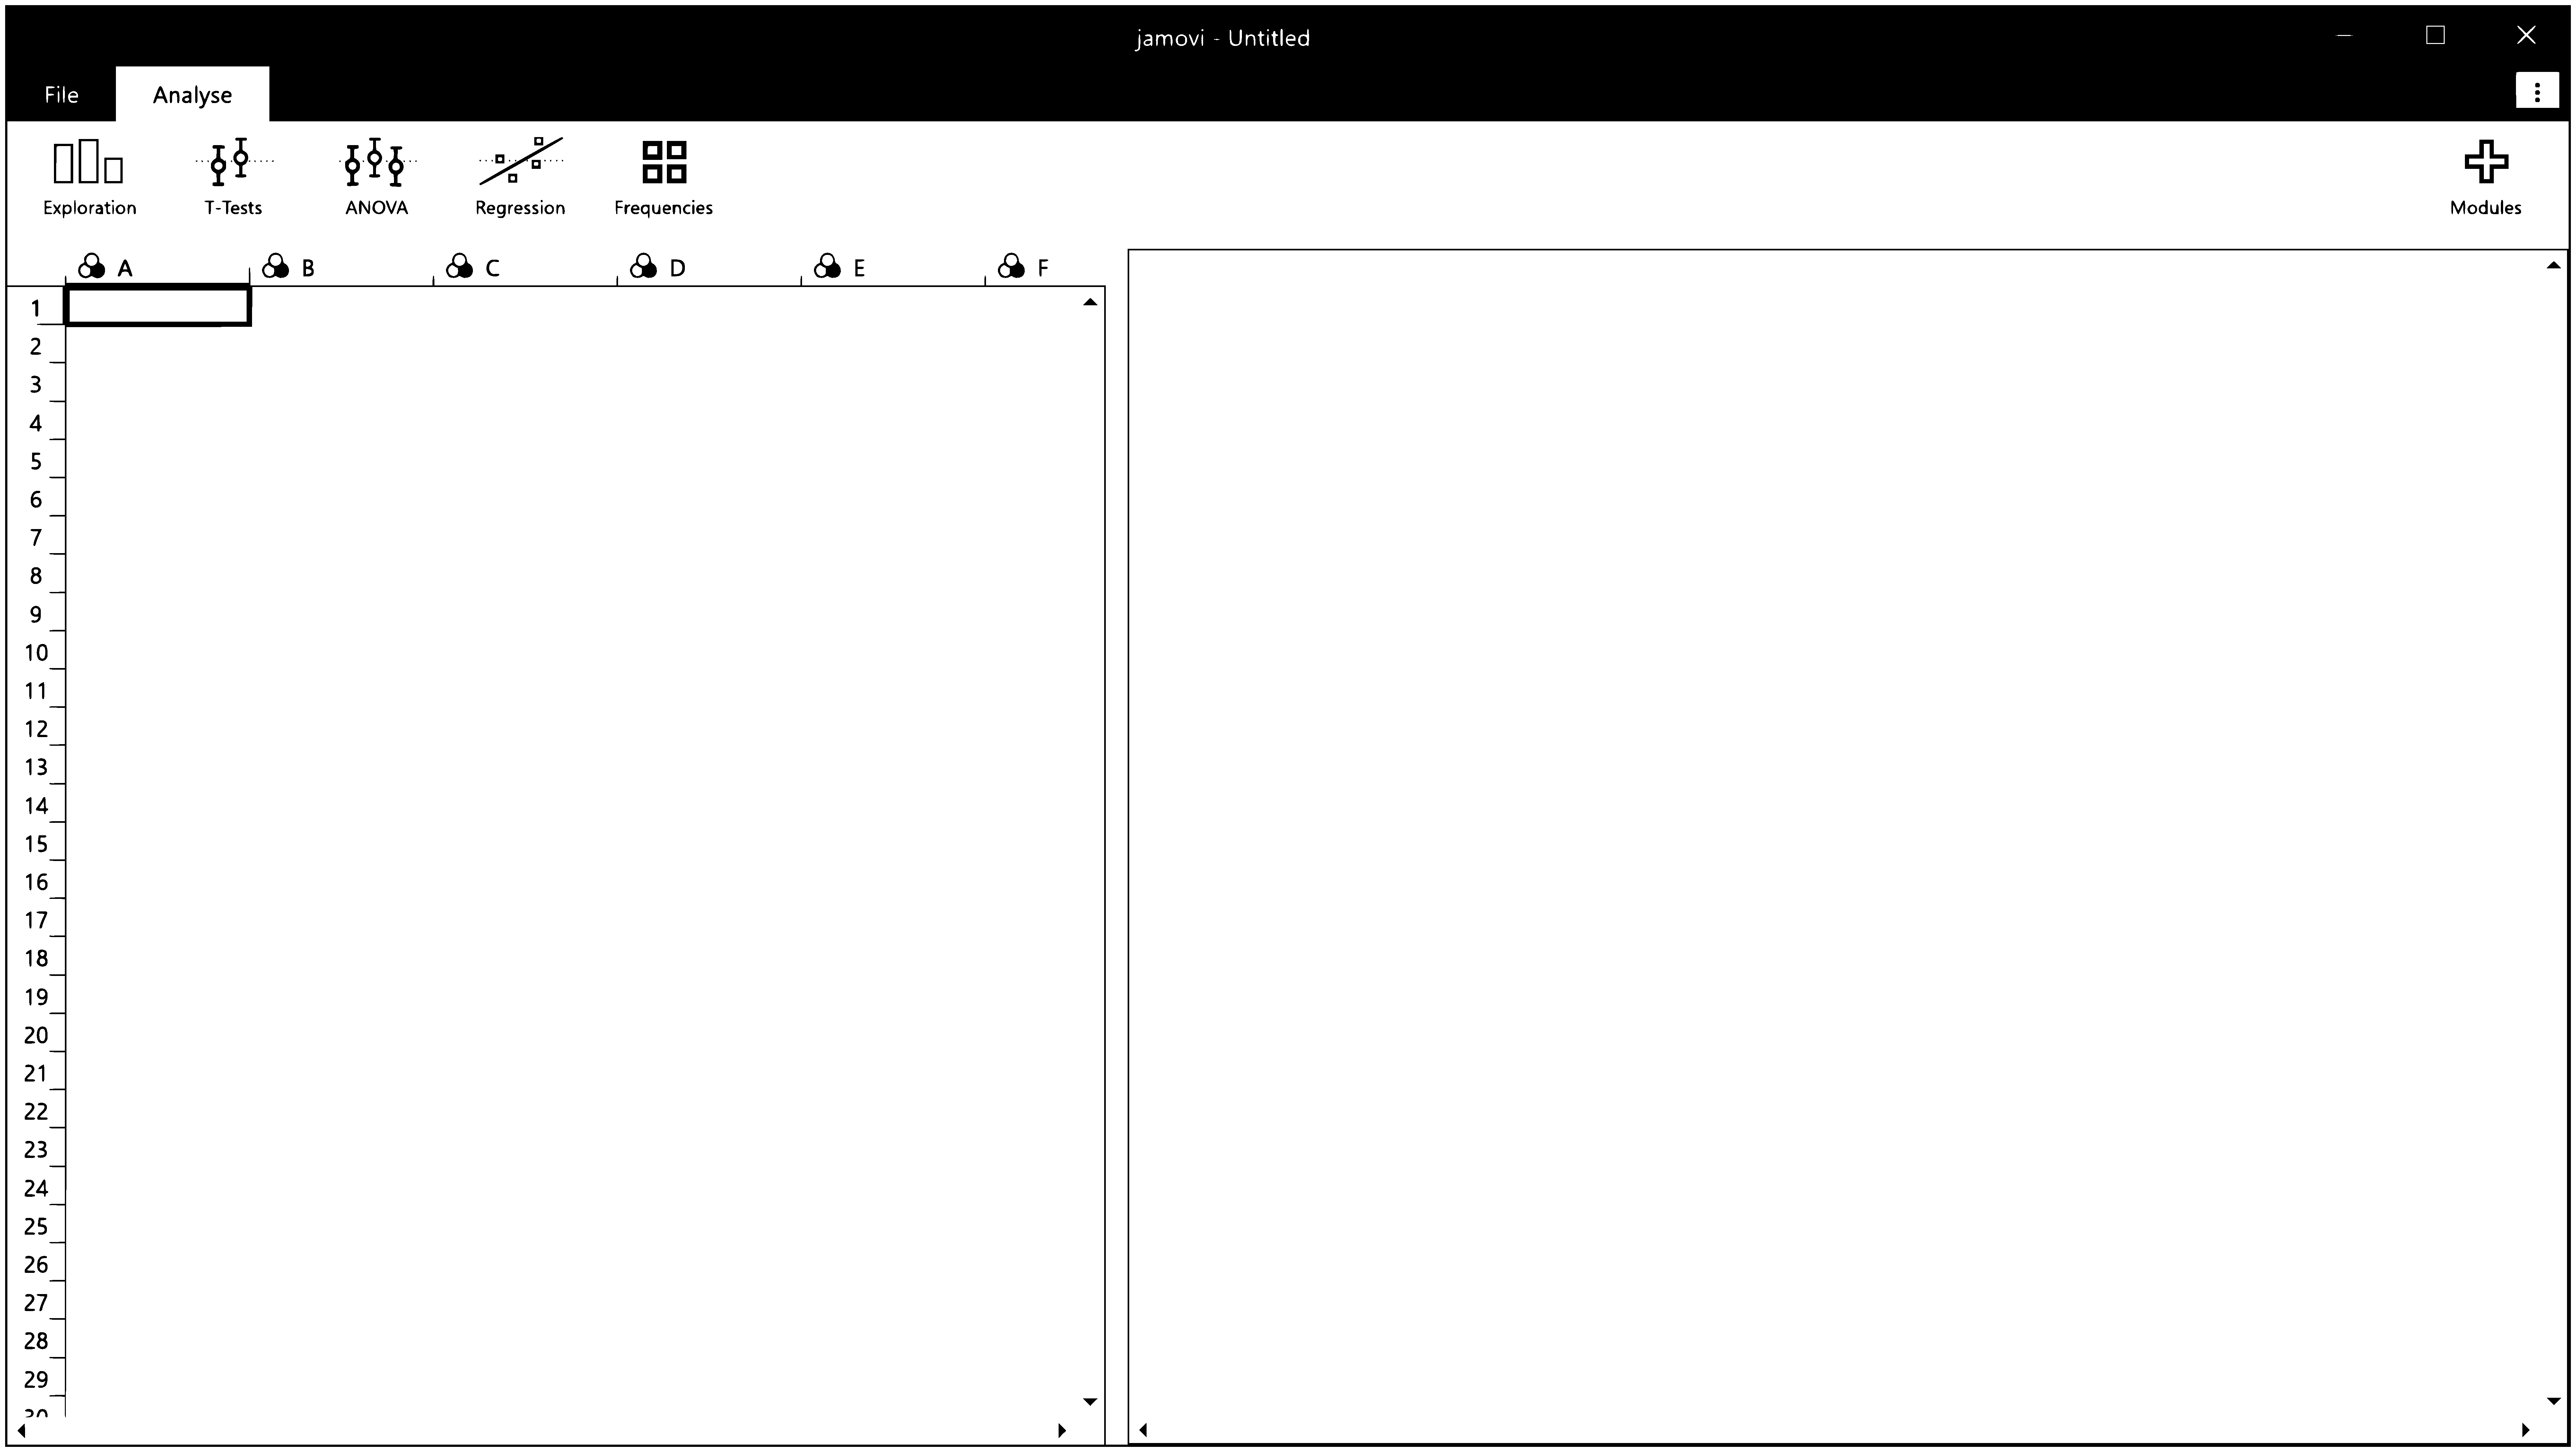
\epsfig{file=../img/introj/startingjamovi.png,clip=true,width=14cm}
\caption{jamovi looks like this when you start it.}
%\HR
\label{fig:startingjamovi}
\end{center}
\end{figure}

To the left is the spreadsheet view, and to the right is where the results of statistical tests appear. Down the middle is a bar separating these two regions and this can be dragged to the left or the right to change their sizes. 

It is possible to simply begin typing values into the jamovi spreadsheet as you would in any other spreadsheet software. Alternatively, existing data sets in the CSV (.csv) file format can be opened in jamovi. Additionally, you can easily import SPSS, SAS, Stata and JASP files directly into jamovi. To open a file select the File tab (three horizontal lines signify this tab) at the top left hand corner, select ‘Open’ and then choose from the files listed on 'Browse' depending on whether you want to open an example or a file stored on your computer.


\section{Analyses\label{sec:analyses}}

Analyses can be selected from the analysis ribbon or menu along the top. Selecting an analysis will present an ‘options panel’ for that particular analysis, allowing you to assign different variables to different parts of the analysis, and select different options. At the same time, the results for the analysis will appear in the right ‘Results panel’ and will update in real-time as you make changes to the options.

When you have the analysis set up correctly you can dismiss the analysis options by clicking the arrow to the top right of the optional panel. If you wish to return to these options, you can click on the results that were produced. In this way, you can return to any analysis that you (or say, a colleague) created earlier.

If you decide you no longer need a particular analysis, you can remove it with the results context menu. Right-clicking on the analysis results will bring up a menu and by selecting ‘Analysis’ and then ‘Remove’ the analysis can be removed. But more on this later. First, let's take a more detailed look at the spreadsheet view.


\section{The spreadsheet\label{sec:spreadsheet}}

In jamovi data is represented in a spreadsheet with each column representing a ‘variable’ and each row representing a ‘case’ or ‘participant’.

\SUBSECTION{Variables}

The most commonly used variables in jamovi are ‘Data Variables’, these variables simply contain data either loaded from a data file, or ‘typed in’ by the user. Data variables can be one of three measurement levels:

\begin{figure}[ht]
\epsfig{file=../img/introj/measurementlevels.png, width = 12cm}
\end{figure}

These levels are designated by the symbol in the header of the variable’s column.

The {\it ID} variable type is unique to jamovi. It’s intended for variables that contain identifiers that you would almost never want to analyse. For example, a persons name, or a participant ID. Specifying an ID variable type can improve performance when interacting with very large data sets.

{\it Nominal} variables are for categorical variables which are text labels, for example a column called Gender with the values Male and Female would be nominal. So would a person’s name. Nominal variable values can also have a numeric value. These variables are used most often when importing data which codes values with numbers rather than text. For example, a column in a dataset may contain the values 1 for males, and 2 for females. It is possible to add nice ‘human-readable’ labels to these values with the variable editor (more on this later).

{\it Ordinal} variables are like Nominal variables, except the values have a specific order. An example is a Likert scale with 3 being ‘strongly agree’ and -3 being ‘strongly disagree’.

{\it Continuous} variables are variables which exist on a continuous scale. Examples might be height or weight. This is also referred to as ‘Interval’ or ‘Ratio scale’.

In addition, you can also specify different data types: variables have a data type of either ‘Text’, ‘Integer’ or ‘Decimal’. 

When starting with a blank spreadsheet and typing values in the variable type will change automatically depending on the data you enter. This is a good way to get a feel for which variable types go with which sorts of data. Similarly, when opening a data file jamovi will try and guess the variable type from the data in each column. In both cases this automatic approach may not be correct, and it may be necessary to manually specify the variable type with the variable editor.

The variable editor can be opened by selecting ‘Setup’ from the data tab or by double-clicking on the variable column header. The variable editor allows you to change the name of the variable and, for data variables, the variable type, the order of the levels, and the label displayed for each level. Changes can be applied by clicking the ‘tick’ to the top right. The variable editor can be dismissed by clicking the `Hide' arrow.

New variables can be inserted or appended to the data set using the ‘add’ button from the data ribbon. The ‘add’ button also allows the addition of computed variables.

\SUBSECTION{Computed variables}

Computed Variables are those which take their value by performing a computation on other variables. Computed Variables can be used for a range of purposes, including log transforms, z-scores, sum-scores, negative scoring and means.

Computed variables can be added to the data set with the ‘add’ button available on the data tab. This will produce a formula box where you can specify the formula. The usual arithmetic operators are available. Some examples of formulas are:

A + B

LOG10(len)

MEAN(A, B)

(dose - VMEAN(dose)) / VSTDEV(dose)

In order, these are the sum of A and B, a log (base 10) transform of len, the mean of A and B, and the z-score of the variable dose. Figure \ref{fig:computedvariable} below shows the jamovi screen for the new variable computed as the z-score of dose (from the `Tooth Growth' example data set).

\vspace*{1cm}
\begin{figure}[ht]
\begin{center}
\epsfig{file=../img/introj/computedvariable.png,clip=true,width=14cm}
\caption{A newly computed variable, the z-score of `dose'.}
\HR
\label{fig:computedvariable}
\end{center}
\end{figure}


{\it V-functions}

Several functions are already available in jamovi and available from the drop down box labelled {\it f\textsubscript{x}}. A number of functions appear in pairs, one prefixed with a V and the other not. V functions perform their calculation on a variable as a whole, where as non-V functions perform their calculation row by row. For example, MEAN(A, B) will produce the mean of A and B for each row. Where as VMEAN(A) gives the mean of all the values in A.

\SUBSECTION{Copy and Paste\label{sec:copypaste}}

jamovi produces nice American Psychological Association (APA) formatted tables and attractive plots. It is often useful to be able to copy and paste these, perhaps into a Word document, or into an email to a colleague. To copy results right click on the object of interest and from the menu select exactly what you want to copy. The menu allows you to choose to copy only the image or the entire analysis. Selecting ``copy'' copies the content to the clipboard and this can be pasted into other programs in the usual way. You can practice this later on when we do some analyses.

\SUBSECTION{Syntax mode\label{sec:syntaxmode}}

jamovi also provides an “\R\ Syntax Mode”. In this mode jamovi produces equivalent \R\ code for each analysis. To change to syntax mode, select the Application menu to the top right of jamovi (a button with three vertical dots) and click the “Syntax mode” checkbox there. You can turn off syntax mode by clicking this a second time.

In syntax mode analyses continue to operate as before but now they produce \R\ syntax, and `ascii output’ like an \R\ session. Like all results objects in jamovi, you can right click on these items (including the \R\ syntax) and copy and paste them, for example into an \R\ session. At present, the provided \R\ syntax does not include the data import step and so this must be performed manually in \R. There are many resources explaining how to import data into \R\ and if you are interested we recommend you take a look at these; just search on the interweb. 


\section{Loading data in jamovi\label{sec:load}}

There are several different types of files that are likely to be relevant to us when doing data analysis. There are two in particular that are especially important from the perspective of this book:
\begin{itemize}
\item {\it jamovi files} are those with a \filename{.omv} file extension. This is the standard kind of file that jamovi uses to store data, and variables and analyses. 
\item {\it Comma separated value (csv) files} are those with a \filename{.csv} file extension. These are just regular old text files and they can be opened with many different software programs. It's quite typical for people to store data in csv files, precisely because they're so simple.
\end{itemize} 

There are also several other kinds of data file that you might want to import into jamovi. For instance, you might want to open Microsoft Excel spreadsheets (\filename{.xls} files), or data files that have been saved in the native file formats for other statistics software, such as SPSS or SAS.  Whichever file formats you are using, it's a good idea to create a folder or folders especially for your jamovi data sets and analyses and to make sure you keep these backed up regularly. 

\SUBSECTION{Importing data from csv files}

One quite commonly used data format is the humble ``comma separated value'' file, also called a csv file, and usually bearing the file extension \filename{.csv}. csv files are just plain old-fashioned text files and what they store is basically just a table of data. This is illustrated in Figure~\ref{fig:booksalescsv}, which shows a file called \filename{booksales.csv} that I've created. As you can see, each row represents the book sales data for one month. The first row doesn't contain actual data though, it has the names of the variables.

\begin{figure}
\begin{center}
\epsfig{file = ../img/mechanics/booksalescsv.eps, clip=true,width = 14cm}
\caption{The \filename{booksales.csv} data file. On the left I've opened the file using a spreadsheet program (OpenOffice), which shows that the file is basically a table. On the right the same file is open in a standard text editor (the TextEdit program on a Mac), which shows how the file is formatted. The entries in the table are wrapped in quote marks and separated by commas.}
\HR
\label{fig:booksalescsv}
\end{center}
\end{figure} 

It's easy to open csv files in jamovi. From the top left menu (the button with three parallel lines) choose `Open' and browse to where you have stored the csv file on your computer. If you're on a Mac, it'll look like the usual Finder window that you use to choose a file; on Windows it looks like an Explorer window. An example of what it looks like on a Mac is shown in Figure~\ref{fig:fileopen}. I'm assuming that you're familiar with your own computer, so you should have no problem finding the csv file that you want to import! Find the one you want, then click on the ``Open'' button. 

\begin{figure}[t]
\begin{center}
\epsfig{file = ../img/mechanics/openscreen.eps,clip=true, width = 14cm}
\caption{A dialog box on a Mac asking you to select the csv file jamovi should try to import. Mac users will recognise this immediately, it's the usual way in which a Mac asks you to find a file. Windows users won't see this, instead they'll see the usual explorer window that Windows always gives you when it wants you to select a file.}
\HR
\label{fig:fileopen}
\end{center}
\end{figure} 

There are a few things that you can check to make sure that the data gets imported correctly: 

\begin{itemize}
\item Heading. Does the first row of the file contain the names for each variable - a `header' row? The \texttt{booksales.csv} file has a header, so that's a yes.
\item Separator. What character is used to separate different entries? In most csv files this will be a comma (it is ``comma separated'' after all).
\item Decimal. What character is used to specify the decimal point? In English speaking countries this is almost always a period (i.e., \texttt{.}). That's not universally true though, many European countries use a comma. 
\item Quote. What character is used to denote a block of text? That's usually going to be a double quote mark (\rtext{"}). It is for the \texttt{booksales.csv} file.
\end{itemize}


\section{Importing unusual data files~\label{sec:importing}}

Throughout this book I've assumed that your data are stored as a jamovi \filename{.omv} file or as a ``properly'' formatted csv file. However, in real life that's not a terribly plausible assumption to make so I'd better talk about some of the other possibilities that you might run into. 


\SUBSECTION{Loading data from text files} 

The first thing I should point out is that if your data are saved as a text file but aren't {\it quite} in the proper csv format then there's still a pretty good chance that jamovi will be able to open it. You just need to try it and see if it works. Sometimes though you will need to change some of the formatting. The ones that I've often found myself needing to change are:
\begin{itemize}
\item \rtext{header}. A lot of the time when you're storing data as a csv file the first row actually contains the column names and not data. If that's not true then it's a good idea to open up the csv file in a spreadsheet programme such as Open Office and add the header row manually. 
\item \rtext{sep}. As the name ``comma separated value'' indicates, the values in a row of a csv file are usually separated by commas. This isn't universal, however. In Europe the decimal point is typically written as \rtext{,} instead of \rtext{.} and as a consequence it would be somewhat awkward to use \rtext{,} as the separator. Therefore it is not unusual to use \rtext{;} instead of \rtext{,} as the separator. At other times, I've seen a TAB character used. 
\item \rtext{quote}. It's conventional in csv files to include a quoting character for textual data. As you can see by looking at the \filename{booksales.csv} file, this is usually a double quote character, \rtext{"}. But sometimes there is no quoting character at all, or you might see a single quote mark \rtext{'} used instead. 
\item \rtext{skip}. It's actually very common to receive CSV files in which the first few rows have nothing to do with the actual data. Instead, they provide a human readable summary of where the data came from, or maybe they include some technical info that doesn't relate to the data. 
\item \rtext{missing values}. Often you'll get given data with missing values. For one reason or another, some entries in the table are missing. The data file needs to include a ``special'' value to indicate that the entry is missing. By default jamovi assumes that this value is \rtext{99}\FOOTNOTE{You can change the default value for missing values in jamovi from the top right menu (three vertical dots), but this only works at the time of importing data files into jamovi. The default missing value in the dataset should not be a valid number associated with any of the variables, e.g. you could use \rtext{-9999} as this is unlikely to be a valid value.}, for both numeric and text data, so you should make sure that, where necessary, all missing values in the csv file are replaced with \rtext{99} (or \rtext{-9999}; whichever you choose) before opening / importing the file into jamovi. Once you have opened / imported the file into jamovi all the missing values are converted to blank cells in the jamovi spreadsheet view.
\end{itemize}

\SUBSECTION{Loading data from SPSS (and other statistics packages)}

The commands listed above are the main ones we'll need for data files in this book. But in real life we have many more possibilities. For example, you might want to read data files in from other statistics programs. Since SPSS is probably the most widely used statistics package in psychology, it's worth mentioning that jamovi can also import SPSS data files (file extension \filename{.sav}). Just follow the instructions above for how to open a csv file, but this time navigate to the .sav file you want to import. For SPSS files, jamovi will regard all values as missing if they are regarded as ``system missing'' files in SPSS. The `Default missings' value does not seem to work as expected when importing SPSS files, so be aware of this - you might need another step: import the SPSS file into jamovi, then export as a csv file before re-opening in jamovi.\FOOTNOTE{I know this is a bot of a fudge, but it does work and hopefully this will be fixed in a later version of jamovi.}.

And that's pretty much it, at least as far as SPSS goes.  As far as other statistical software goes, jamovi can also directly open / import SAS and STATA files. 

\SUBSECTION{Loading Excel files} 

A different problem is posed by Excel files. Despite years of yelling at people for sending data to me encoded in a proprietary data format, I get sent a lot of Excel files. The way to handle Excel files is to open them up first in Excel or another spreadsheet programme that can handle Excel files, and then export the data as a csv file before opening / importing the csv file into jamovi. 


\section{Changing data from one level to another\label{sec:coercion}}

Sometimes you want to change the variable level. This can happen for all sorts of reasons. Sometimes when you import data from files, it can come to you in the wrong format. Numbers sometimes get imported as nominal, text values. Dates may get imported as text. ParticipantID values can sometimes be read as continuous: nominal values can sometimes be read as ordinal or even continuous. There's a good chance that sometimes you'll want to convert a variable from one measurement level into another one. Or, to use the correct term, you want to \keyterm{coerce} the variable from one class into another. 

In \ref{sec:spreadsheet} we saw how to specify different variable levels, and if you want to change a variable's measurement level then you can do this in the jamovi data view for that variable. Just click the check box for the measurement level you want - continuous, ordinal, or nominal. 


\section{Installing add-on modules into jamovi \label{sec:jamovimodules}}

A really great feature of jamovi is the ability to install add-on modules from the jamovi library. These add-on modules have been developed by the jamovi community, i.e., jamovi users and developers who have created special software add-ons that do other, usually more advanced, analyses that go beyond the capabilities of the base jamovi program. 

To install add-on modules, just click on the large \large{``+''} in the top right of the jamovi window, select ``jamovi-library'' and then browse through the various add-on modules that are available. Choose the one(s) you want, and then install them, as in Figure \ref{fig:modules}. It's that easy. The newly installed modules can then be accessed from the ``Analyses'' button bar. Try it...useful add-on modules to install include ''scatr'' (added under ``Descriptives'') and ``\R\ j''. 

\begin{figure}[htb]
\begin{center}
\epsfig{file = ../img/graphics/modules.png, clip=true,width =14cm} 
\caption{Installing add-on modules in jamovi}
\label{fig:modules}
\HR
\end{center}
\end{figure}


\section{Quitting jamovi \label{sec:quittingjamovi}}

There's one last thing I should cover in this chapter: how to quit jamovi. It's not hard, just close the program the same way you would any other program. However, what you might want to do before you quit is save your work! There are two parts to this: saving any changes to the data set, and saving the analyses that you ran.

It is good practice to save any changes to the data set as a {\it new} data set. That way you can always go back to the original data. To save any changes in jamovi, select `Export'...`Data' from the main jamovi menu (button with three horizontal bars in the top left) and create a new file name for the changed data set.

Alternatively, you can save {\it both} the changed data and any analyses you have undertaken by saving as a jamovi file. To do this, from the main jamovi menu select `Save as' and type in a file name for this `jamovi file (.omv)'. Remember to save the file in a location where you can find it again later. I usually create a new folder for specific data sets and analyses.  


\section{Summary}

Every book that tries to teach a new statistical software program to novices has to cover roughly the same topics, and in roughly the same order. Ours is no exception, and so in the grand tradition of doing it just the same way everyone else did it, this chapter covered the following topics:

\begin{itemize}
\item Section~\ref{sec:gettingjamovi}. We downloaded and installed jamovi, and started it up.
\item Section~\ref{sec:analyses}. We very briefly oriented to the part of jamovi where analyses are done and results appear, but then deferred this until later in the book.
\item Section~\ref{sec:spreadsheet}. We spent more time looking at the spreadsheet part of jamovi, and considered different variable types, and how to compute new variables.
\item Section~\ref{sec:load}. We also saw how to load data files in jamovi.
\item Section~\ref{sec:importing}. Then we figured out how to open other data files, from different file types.
\item Section~\ref{sec:coercion}. And saw that sometimes we need to coerce data from one type to another.
\item Section~\ref{sec:jamovimodules}. Installing add-on modules from the jamovi community really extends jamovi capabilities.
\item Section~\ref{sec:quittingjamovi}. Finally, we looked at good practice in terms of saving your data set and analyses when you have finished and are about to quit jamovi.
\end{itemize}

\noindent
We still haven't arrived at anything that resembles data analysis. Maybe the next Chapter will get us a bit closer!





\part{Working with data}

% !TEX root = ../pdf/lsj.tex
% [There are multiple lsj.tex files, but the one in ../pdf is the usual one]

%%%%%%%%%%%%%%%%%%%%%%%%%%%%%%%%%%%%%%%%%%%%%%%
\chapter{Descriptive statistics\label{ch:descriptives}}

Any time that you get a new data set to look at one of the first tasks that you have to do is find ways of summarising the data in a compact, easily understood fashion. This is what \keyterm{descriptive statistics} (as opposed to inferential statistics) is all about. In fact, to many people the term ``statistics'' is synonymous with descriptive statistics. It is this topic that we'll consider in this chapter, but before going into any details, let's take a moment to get a sense of why we need descriptive statistics. To do this, let's open the \filename{aflsmall\_margins} file and see what variables are stored in the file.

\vspace{0.5cm}
\begin{figure}[htb]
\begin{center}
\epsfig{file=../img/descriptives/aflsmall_margins.png,clip=true,width=14cm} 
\caption{A screenshot of jamovi showing the variables stored in the \filename{aflsmall\_margins.csv} file}
\label{fig:aflsmall}
\HR
\end{center}
\end{figure}

In fact, there is just one variable here, \rtext{afl.margins}. We'll focus a bit on this variable in this chapter, so I'd better tell you what it is. Unlike most of the data sets in this book, this is actually real data, relating to the Australian Football League (AFL).\FOOTNOTE{Note for non-Australians: the AFL is an Australian rules football competition. You don't need to know anything about Australian rules in order to follow this section.} The \rtext{afl.margins} variable contains the winning margin (number of points) for all 176 home and away games played during the 2010 season. 

This output doesn't make it easy to get a sense of what the data are actually saying. Just ``looking at the data'' isn't a terribly effective way of understanding data. In order to get some idea about what the data are actually saying we need to calculate some descriptive statistics (this chapter) and draw some nice pictures (Chapter~\ref{ch:graphics}). Since the descriptive statistics are the easier of the two topics I'll start with those, but nevertheless I'll show you a histogram of the \rtext{afl.margins} data since it should help you get a sense of what the data we're trying to describe actually look like, see Figure~\ref{fig:histogram1}. We'll talk a lot more about how to draw histograms in Section~\ref{sec:hist}. For now, it's enough to look at the histogram and note that it provides a fairly interpretable representation of the \rtext{afl.margins} data.

\begin{figure}[ht]
\begin{center}
\epsfig{file=../img/descriptives/aflMargins.eps,clip=true,width=12cm} 
\caption{A histogram of the AFL 2010 winning margin data (the \rtext{afl.margins} variable). As you might expect, the larger the winning margin the less frequently you tend to see it.}
\label{fig:histogram1}
\HR
\end{center}
\end{figure}

\section{Measures of central tendency~\label{sec:centraltendency}}

Drawing pictures of the data, as I did in Figure~\ref{fig:histogram1}, is an excellent way to convey the ``gist'' of what the data is trying to tell you. It's often extremely useful to try to condense the data into a few simple ``summary'' statistics. In most situations, the first thing that you'll want to calculate is a measure of \keyterm{central tendency}. That is, you'd like to know something about where the ``average'' or ``middle'' of your data lies. The three most commonly used measures are the mean, median and mode. I'll explain each of these in turn, and then discuss when each of them is useful.

\SUBSECTION{The mean\label{sec:mean}}

The \keyterm{mean} of a set of observations is just a normal, old-fashioned average. Add all of the values up, and then divide by the total number of values. The first five AFL winning margins were 56, 31, 56, 8 and 32, so the mean of these observations is just:
$$
\frac{56 + 31 + 56 + 8 + 32}{5} = \frac{183}{5} = 36.60
$$
Of course, this definition of the mean isn't news to anyone. Averages (i.e., means) are used so often in everyday life that this is pretty familiar stuff. However, since the concept of a mean is something that everyone already understands, I'll use this as an excuse to start introducing some of the mathematical notation that statisticians use to describe this calculation, and talk about how the calculations would be done in jamovi. 

The first piece of notation to introduce is $N$, which we'll use to refer to the number of observations that we're averaging (in this case $N = 5$). Next, we need to attach a label to the observations themselves. It's traditional to use $X$ for this, and to use subscripts to indicate which observation we're actually talking about. That is, we'll use $X_1$ to refer to the first observation, $X_2$ to refer to the second observation, and so on all the way up to $X_N$ for the last one. Or, to say the same thing in a slightly more abstract way, we use $X_i$ to refer to the $i$-th observation. Just to make sure we're clear on the notation, the following table lists the 5 observations in the \rtext{afl.margins} variable, along with the mathematical symbol used to refer to it and the actual value that the observation corresponds to:

\begin{center}
\begin{tabular}{ccc}
the observation & its symbol & the observed value \\ \hline
winning margin, game 1 & $X_1$ & 56 points \\
winning margin, game 2 & $X_2$ & 31 points \\
winning margin, game 3 & $X_3$ & 56 points \\
winning margin, game 4 & $X_4$ & 8 points \\
winning margin, game 5 & $X_5$ & 32 points \\
\end{tabular}
\end{center}

%\noindent
\vspace{0.5cm}
\begin{mdframed}[style=MyFrame,nobreak=true]
Okay, now let's try to write a formula for the mean. By tradition, we use $\bar{X}$ as the notation for the mean. So the calculation for the mean could be expressed using the following formula:
$$
\bar{X} = \frac{X_1 + X_2 + \ldots + X_{N-1} + X_N}{N}
$$
This formula is entirely correct but it's terribly long, so we make use of the \keyterm{summation symbol} $\scriptstyle\sum$ to shorten it.\FOOTNOTE{The choice to use $\Sigma$ to denote summation isn't arbitrary. It's the Greek upper case letter sigma, which is the analogue of the letter S in that alphabet. Similarly, there's an equivalent symbol used to denote the multiplication of lots of numbers, because multiplications are also called ``products'' we use the $\Pi$ symbol for this (the Greek upper case pi, which is the analogue of the letter P).} If I want to add up the first five observations I could write out the sum the long way, $X_1 + X_2 + X_3 + X_4 +X_5$ or I could use the summation symbol to shorten it to this:
$$
\sum_{i=1}^5 X_i
$$
Taken literally, this could be read as ``the sum, taken over all $i$ values from 1 to 5, of the value $X_i$''. But basically what it means is ``add up the first five observations''. In any case, we can use this notation to write out the formula for the mean, which looks like this:
$$
\bar{X} = \frac{1}{N} \sum_{i=1}^N X_i 
$$

In all honesty, I can't imagine that all this mathematical notation helps clarify the concept of the mean at all. In fact, it's really just a fancy way of writing out the same thing I said in words: add all the values up and then divide by the total number of items. However, that's not really the reason I went into all that detail. My goal was to try to make sure that everyone reading this book is clear on the notation that we'll be using throughout the book: $\bar{X}$ for the mean, $\scriptstyle\sum$ for the idea of summation, $X_i$ for the $i$th observation, and $N$ for the total number of observations. We're going to be re-using these symbols a fair bit so it's important that you understand them well enough to be able to ``read'' the equations, and to be able to see that it's just saying ``add up lots of things and then divide by another thing''.
\end{mdframed}

\SUBSECTION{Calculating the mean in jamovi}

Okay, that's the maths. So how do we get the magic computing box to do the work for us? When the number of observations starts to become large it's much easier to do these sorts of calculations using a computer. To calculate the mean using all the data we can use jamovi. The first step is to click on the `Exploration' button and then click `Descriptives'. Then you can highlight the \rtext{afl.margins} variable and click the `right arrow' to move it across into the `Variables box'. As soon as you do that a Table appears on the right hand side of the screen containing default `Descriptives' information; see Figure \ref{fig:descriptives_default}. 

\vspace{0.5cm}
\begin{figure}[ht]
\begin{center}
\epsfig{file=../img/descriptives/descriptives_default.png,clip=true,width=12cm} 
\caption{Default descriptives for the AFL 2010 winning margin data (the \rtext{afl.margins} variable). }
\label{fig:descriptives_default}
\HR
\end{center}
\end{figure}

As you can see in Figure \ref{fig:descriptives_default}, the mean value for the \rtext{afl.margins} variable is 35.30. Other information presented includes the total number of observations (N=176), the number of missing values (none), and the Median, Minimum and Maximum values for the variable. 

\SUBSECTION{The median\label{sec:median}}

The second measure of central tendency that people use a lot is the \keyterm{median}, and it's even easier to describe than the mean. The median of a set of observations is just the middle value. As before let's imagine we were interested only in the first 5 AFL winning margins: 56, 31, 56, 8 and 32. To figure out the median we sort these numbers into ascending order:
$$
8, 31, \mathbf{32}, 56, 56
$$
From inspection, it's obvious that the median value of these 5 observations is 32 since that's the middle one in the sorted list (I've put it in bold to make it even more obvious). Easy stuff. But what should we do if we are interested in the first 6 games rather than the first 5? Since the sixth game in the season had a winning margin of 14 points, our sorted list is now 
$$
8, 14, \mathbf{31}, \mathbf{32}, 56, 56
$$
and there are {\it two} middle numbers, 31 and 32. The median is defined as the average of those two numbers, which is of course 31.5. As before, it's very tedious to do this by hand when you've got lots of numbers. In real life, of course, no-one actually calculates the median by sorting the data and then looking for the middle value. In real life we use a computer to do the heavy lifting for us, and jamovi has provided us with a Median value of 30.50 for the \rtext{afl.margins} variable (Figure~\ref{fig:descriptives_default}). 

\SUBSECTION{Mean or median? What's the difference?}

Knowing how to calculate means and medians is only a part of the story. You also need to understand what each one is saying about the data, and what that implies for when you should use each one. This is illustrated in Figure~\ref{fig:meanmedian}. The mean is kind of like the ``centre of gravity'' of the data set, whereas the median is the ``middle value'' in the data. What this implies, as far as which one you should use, depends a little on what type of data you've got and what you're trying to achieve. As a rough guide:
\begin{itemize} 
\item If your data are nominal scale you probably shouldn't be using either the mean or the median. Both the mean and the median rely on the idea that the numbers assigned to values are meaningful. If the numbering scheme is arbitrary then it's probably best to use the mode (Section~\ref{sec:mode}) instead. 
\item If your data are ordinal scale you're more likely to want to use the median than the mean. The median only makes use of the order information in your data (i.e., which numbers are bigger) but doesn't depend on the precise numbers involved. That's exactly the situation that applies when your data are ordinal scale. The mean, on the other hand, makes use of the precise numeric values assigned to the observations, so it's not really appropriate for ordinal data.
\item For interval and ratio scale data either one is generally acceptable. Which one you pick depends a bit on what you're trying to achieve. The mean has the advantage that it uses all the information in the data (which is useful when you don't have a lot of data). But it's very sensitive to extreme, outlying  values.  
\end{itemize}

\vspace{0.5cm}
\begin{figure}[htb]
\begin{center}
\epsfig{file = ../img/descriptives2/mean.eps,clip=true, width = 6cm}
\raisebox{1mm}{\epsfig{file = ./../img/descriptives2/median.eps,clip=true, width = 6.4cm}}
\caption{An illustration of the difference between how the mean and the median should be interpreted. The mean is basically the ``centre of gravity'' of the data set. If you imagine that the histogram of the data is a solid object, then the point on which you could balance it (as if on a see-saw) is the mean. In contrast, the median is the middle observation, with half of the observations smaller and half of the observations larger.}
\HR
\label{fig:meanmedian}
\end{center}
\end{figure}

Let's expand on that last part a little. One consequence is that there are systematic differences between the mean and the median when the histogram is asymmetric (skewed; see Section~\ref{sec:skewkurt}). This is illustrated in Figure~\ref{fig:meanmedian}. Notice that the median (right hand side) is located closer to the ``body'' of the histogram, whereas the mean (left hand side) gets dragged towards the ``tail'' (where the extreme values are). To give a concrete example, suppose Bob (income \$50,000), Kate (income \$60,000) and Jane (income \$65,000) are sitting at a table. The average income at the table is \$58,333 and the median income is \$60,000. Then Bill sits down with them (income \$100,000,000). The average income has now jumped to \$25,043,750 but the median rises only to \$62,500. If you're interested in looking at the overall income at the table the mean might be the right answer. But if you're interested in what counts as a typical income at the table the median would be a better choice here.

\SUBSECTION{A real life example~\label{sec:housingpriceexample}}

To try to get a sense of why you need to pay attention to the differences between the mean and the median let's consider a real life example. Since I tend to mock journalists for their poor scientific and statistical knowledge, I should give credit where credit is due. This is an excellent article on the ABC news website\FOOTNOTE{\url{www.abc.net.au/news/stories/2010/09/24/3021480.htm}} from 24 September, 2010:
\small
\begin{quote}
Senior Commonwealth Bank executives have travelled the world in the past couple of weeks with a presentation showing how Australian house prices, and the key price to income ratios, compare favourably with similar countries. ``Housing affordability has actually been going sideways for the last five to six years,'' said Craig James, the chief economist of the bank's trading arm, CommSec.
\end{quote}
\normalsize
This probably comes as a huge surprise to anyone with a mortgage, or who wants a mortgage, or pays rent, or isn't completely oblivious to what's been going on in the Australian housing market over the last several years. Back to the article:
\small
\begin{quote}
CBA has waged its war against what it believes are housing doomsayers with graphs, numbers and international comparisons. In its presentation, the bank rejects arguments that Australia's housing is relatively expensive compared to incomes. It says Australia's house price to household income ratio of 5.6 in the major cities, and 4.3 nationwide, is comparable to many other developed nations. It says San Francisco and New York have ratios of 7, Auckland's is 6.7, and Vancouver comes in at 9.3.
\end{quote}
\normalsize
More excellent news! Except, the article goes on to make the observation that:
\small
\begin{quote}
Many analysts say that has led the bank to use misleading figures and comparisons. If you go to page four of CBA's presentation and read the source information at the bottom of the graph and table, you would notice there is an additional source on the international comparison -- Demographia. However, if the Commonwealth Bank had also used Demographia's analysis of Australia's house price to income ratio, it would have come up with a figure closer to 9 rather than 5.6 or 4.3
\end{quote}
\normalsize
That's, um, a rather serious discrepancy. One group of people say 9, another says 4-5. Should we just split the difference and say the truth lies somewhere in between? Absolutely not! This is a situation where there is a right answer and a wrong answer. Demographia is correct, and the Commonwealth Bank is wrong. As the article points out:
\small
\begin{quote}
[An] obvious problem with the Commonwealth Bank's domestic price to income figures is they compare average incomes with median house prices (unlike the Demographia figures that compare median incomes to median prices). The median is the mid-point, effectively cutting out the highs and lows, and that means the average is generally higher when it comes to incomes and asset prices, because it includes the earnings of Australia's wealthiest people. To put it another way: the Commonwealth Bank's figures count Ralph Norris' multi-million dollar pay packet on the income side, but not his (no doubt) very expensive house in the property price figures, thus understating the house price to income ratio for middle-income Australians.
\end{quote}
\normalsize
Couldn't have put it better myself. The way that Demographia calculated the ratio is the right thing to do. The way that the Bank did it is incorrect. As for why an extremely quantitatively sophisticated organisation such as a major bank made such an elementary mistake, well... I can't say for sure since I have no special insight into their thinking. But the article itself does happen to mention the following facts, which may or may not be relevant:
\small
\begin{quote}
[As] Australia's largest home lender, the Commonwealth Bank has one of the biggest vested interests in house prices rising. It effectively owns a massive swathe of Australian housing as security for its home loans as well as many small business loans.
\end{quote}
\normalsize
My, my. 

\SUBSECTION{Mode\label{sec:mode}}

The mode of a sample is very simple. It is the value that occurs most frequently. We can illustrate the mode using a different AFL variable: who has played in the most finals? Open the \filename{aflsmall\_finalists} file and take a look at the \rtext{afl.finalists} variable, see Figure \ref{fig:aflsmall_finalists}. This variable contains the names of all 400 teams that played in all 200 finals matches played during the period 1987 to 2010. 

%\vspace{0.5cm}
\begin{figure}[!!htp]
\begin{center}
\epsfig{file=../img/descriptives/aflsmall_finalists.png,clip=true,width=11cm} 
\caption{A screenshot of jamovi showing the variables stored in the \filename{aflsmall\_finalists.csv} file}
\label{fig:aflsmall_finalists}
\HR
\end{center}
\end{figure}

What we {\it could} do is read through all 400 entries and count the number of occasions on which each team name appears in our list of finalists, thereby producing a \keyterm{frequency table}. However, that would be mindless and boring: exactly the sort of task that computers are great at. So let's use jamovi to do this for us. Under `Exploration' - `Descriptives' click the small check box labelled `Frequency tables' and you should get something like Figure \ref{fig:aflsmall_finalists_mode}. 

%\vspace{0.5cm}
\begin{figure}[!!htp]
\begin{center}
\epsfig{file=../img/descriptives/aflsmall_finalists_mode.png,clip=true,width=12cm} 
\caption{A screenshot of jamovi showing the frequency table for the \rtext{afl.finalists} variable }
\label{fig:aflsmall_finalists_mode}
\HR
\end{center}
\end{figure}

Now that we have our frequency table we can just look at it and see that, over the 24 years for which we have data, Geelong has played in more finals than any other team. Thus, the mode of the \rtext{afl.finalists} data is \rtext{"Geelong"}. We can see that Geelong (39 finals) played in more finals than any other team during the 1987-2010 period. It's also worth noting that in the `Descriptives' Table no results are calculated for Mean, Median, Minimum or Maximum. This is because the \rtext{afl.finalists} variable is a nominal text variable so it makes no sense to calculate these values.

One last point to make regarding the mode. Whilst the mode is most often calculated when you have nominal data, because means and medians are useless for those sorts of variables, there are some situations in which you really do want to know the mode of an ordinal, interval or ratio scale variable. For instance, let's go back to our \rtext{afl.margins} variable. This variable is clearly ratio scale (if it's not clear to you, it may help to re-read Section~\ref{sec:scales}), and so in most situations the mean or the median is the measure of central tendency that you want. But consider this scenario: a friend of yours is offering a bet and they pick a football game at random. Without knowing who is playing you have to guess the {\it exact} winning margin. If you guess correctly you win \$50. If you don't you lose \$1. There are no consolation prizes for ``almost'' getting the right answer. You have to guess exactly the right margin. For this bet, the mean and the median are completely useless to you. It is the mode that you should bet on. To calculate the mode for the \rtext{afl.margins} variable in jamovi, go back to that data set and on the `Exploration' - `Descriptives' screen you will see you can expand the section marked `Statistics'. Click on the checkbox marked `Mode' and you will see the modal value presented in the `Descriptives' Table, as in Figure \ref{fig:aflsmall_margins_mode}. So the 2010 data suggest you should bet on a 3 point margin.

\vspace{0.5cm}
\begin{figure}[!!htb]
\begin{center}
\epsfig{file=../img/descriptives/aflsmall_margins_mode.png,clip=true,width=12cm} 
\caption{A screenshot of jamovi showing the modal value for the \rtext{afl.margins} variable }
\label{fig:aflsmall_margins_mode}
\HR
\end{center}
\end{figure}


\section{Measures of variability\label{sec:var}}

The statistics that we've discussed so far all relate to {\it central tendency}. That is, they all talk about which values are ``in the middle'' or ``popular'' in the data. However, central tendency is not the only type of summary statistic that we want to calculate. The second thing that we really want is a measure of the \keyterm{variability} of the data. That is, how ``spread out'' are the data? How ``far'' away from the mean or median do the observed values tend to be? For now, let's assume that the data are interval or ratio scale, and we'll continue to use the \rtext{afl.margins} data.  We'll use this data to discuss several different measures of spread, each with different strengths and weaknesses. 

\SUBSECTION{Range\label{sec:range}}

The \keyterm{range} of a variable is very simple. It's the biggest value minus the smallest value. For the AFL winning margins data the maximum value is 116 and the minimum value is 0. Although the range is the simplest way to quantify the notion of ``variability'', it's one of the worst. Recall from our discussion of the mean that we want our summary measure to be robust. If the data set has one or two extremely bad values in it we'd like our statistics to not be unduly influenced by these cases. For example, in a variable containing very extreme outliers 
$$
-100,2,3,4,5,6,7,8,9,10
$$
it is clear that the range is not robust. This variable has a range of 110 but if the outlier were removed we would have a range of only 8.

\SUBSECTION{Interquartile range}

The \keyterm{interquartile range} (IQR) is like the range, but instead of the difference between the biggest and smallest value the difference between the 25th percentile and the 75th percentile is taken. If you don't already know what a \keyterm{percentile} is, the 10th percentile of a data set is the smallest number $x$ such that 10\% of the data is less than $x$. In fact, we've already come across the idea. The median of a data set is its 50th percentile! In jamovi you can easily specify the 25th, 50th and 75th percentiles by clicking the checkbox `Quartiles' in the `Exploration' - `Descriptives' - `Statistics' screen. 

%\vspace{0.5cm}
\begin{figure}[htb]
\begin{center}
\epsfig{file=../img/descriptives/aflsmall_margins_iqr.png,clip=true,width=6cm} 
\caption{A screenshot of jamovi showing the Quartiles for the \rtext{afl.margins} variable }
\label{fig:aflsmall_margins_iqr}
\HR
\end{center}
\end{figure}

And not surprisingly, in Figure \ref{fig:aflsmall_margins_iqr} the 50th percentile is the same as the median value. And, by noting that $50.50 - 12.75 = 37.75$, we can see that the interquartile range for the 2010 AFL winning margins data is 37.75. While it's obvious how to interpret the range it's a little less obvious how to interpret the IQR. The simplest way to think about it is like this: the interquartile range is the range spanned by the ``middle half'' of the data. That is, one quarter of the data falls below the 25th percentile and one quarter of the data is above the 75th percentile, leaving the ``middle half'' of the data lying in between the two. And the IQR is the range covered by that middle half.

\SUBSECTION{Mean absolute deviation~\label{sec:aad}}

The two measures we've looked at so far, the range and the interquartile range, both rely on the idea that we can measure the spread of the data by looking at the percentiles of the data. However, this isn't the only way to think about the problem. A different approach is to select a meaningful reference point (usually the mean or the median) and then report the ``typical'' deviations from that reference point. What do we mean by ``typical'' deviation? Usually, this is the mean or median value of these deviations. In practice, this leads to two different measures: the ``mean absolute deviation'' (from the mean) and the ``median absolute deviation'' (from the median). From what I've read, the measure based on the median seems to be used in statistics and does seem to be the better of the two. But to be honest I don't think I've seen it used much in psychology. The measure based on the mean does occasionally show up in psychology though. In this section I'll talk about the first one, and I'll come back to talk about the second one later.

Since the previous paragraph might sound a little abstract, let's go through the \keyterm{mean absolute deviation} from the mean a little more slowly. One useful thing about this measure is that the name actually tells you exactly how to calculate it. Let's think about our AFL winning margins data, and once again we'll start by pretending that there are only 5 games in total, with winning margins of 56, 31, 56, 8 and 32. Since our calculations rely on an examination of the deviation from some reference point (in this case the mean), the first thing we need to calculate is the mean, $\bar{X}$. For these five observations, our mean is $\bar{X} = 36.6$. The next step is to convert each of our observations $X_i$ into a deviation score. We do this by calculating the difference between the observation $X_i$ and the mean $\bar{X}$. That is, the deviation score is defined to be $X_i - \bar{X}$. For the first observation in our sample, this is equal to $56 - 36.6 = 19.4$. Okay, that's simple enough. The next step in the process is to convert these deviations to absolute deviations, and we do this by converting any negative values to positive ones. Mathematically, we would denote the absolute value of $-3$ as $|-3|$, and so we say that $|-3| = 3$. We use the absolute value here because we don't really care whether the value is higher than the mean or lower than the mean, we're just interested in how {\it close} it is to the mean. To help make this process as obvious as possible, the table below shows these calculations for all five observations:

\vspace{0.5cm}
\begin{center}
\begin{tabular}{ccccc} 
English: & which game & value & deviation from mean & absolute deviation \\
notation: & $i$ & $X_i$ & $X_i - \bar{X}$ &  $|X_i - \bar{X}|$ \\ \hline
& 1 & 56 & 19.4  & 19.4\\
& 2 & 31 &  -5.6 & 5.6\\ 
& 3 & 56 & 19.4  & 19.4\\
& 4 & 8 & -28.6  & 28.6\\
& 5 & 32 & -4.6  & 4.6 \\
\end{tabular}
\end{center}

\noindent
Now that we have calculated the absolute deviation score for every observation in the data set, all that we have to do to calculate the mean of these scores. Let's do that:

$$
\frac{19.4 + 5.6 + 19.4 + 28.6 + 4.6}{5} = 15.52
$$

\noindent
And we're done. The mean absolute deviation for these five scores is 15.52. 

\vspace{0.5cm}
\begin{mdframed}[style=MyFrame,nobreak=true]
However, whilst our calculations for this little example are at an end, we do have a couple of things left to talk about. First, we should really try to write down a proper mathematical formula. But in order do to this I need some mathematical notation to refer to the mean absolute deviation. Irritatingly, ``mean absolute deviation'' and ``median absolute deviation'' have the same acronym (MAD), which leads to a certain amount of ambiguity so I'd better come up with something different for the mean absolute deviation. Sigh. What I'll do is use AAD instead, short for {\it average} absolute deviation. Now that we have some unambiguous notation, here's the formula that describes what we just calculated:
$$
\mbox{\textsc{aad}}(X) = \frac{1}{N} \sum_{i = 1}^N |X_i - \bar{X}|
$$
\end{mdframed}

\SUBSECTION{Variance} 

Although the average absolute deviation measure has its uses, it's not the best measure of variability to use. From a purely mathematical perspective there are some solid reasons to prefer squared deviations rather than absolute deviations. If we do that we obtain a measure called the \keyterm{variance}, which has a lot of really nice statistical properties that I'm going to ignore,\FOOTNOTE{Well, I will very briefly mention the one that I think is coolest, for a very particular definition of ``cool'', that is. Variances are {\it additive}. Here's what that means. Suppose I have two variables $X$ and $Y$, whose variances are $\mbox{Var}(X)$ and $\mbox{Var}(Y)$ respectively. Now imagine I want to define a new variable $Z$ that is the sum of the two, $Z = X+Y$. As it turns out, the variance of $Z$ is equal to $\mbox{Var}(X) + \mbox{Var}(Y)$. This is a {\it very} useful property, but it's not true of the other measures that I talk about in this section.} and one massive psychological flaw that I'm going to make a big deal out of in a moment. The variance of a data set $X$ is sometimes written as $\mbox{Var}(X)$, but it's more commonly denoted $s^2$ (the reason for this will become clearer shortly). 

\vspace{0.5cm}
\begin{mdframed}[style=MyFrame,nobreak=true]
The formula that we use to calculate the variance of a set of observations is as follows:
$$
\mbox{Var}(X) = \frac{1}{N} \sum_{i=1}^N \left( X_i - \bar{X} \right)^2
$$
%\mbox{Var}(X) = \frac{\sum_{i=1}^N \left( X_i - \bar{X} \right)^2}{N}
As you can see, it's basically the same formula that we used to calculate the average absolute deviation, except that instead of using ``absolute deviations'' we use ``squared deviations''. It is for this reason that the variance is sometimes referred to as the ``mean square deviation''.
\end{mdframed}

Now that we've got the basic idea, let's have a look at a concrete example. Once again, let's use the first five AFL games as our data. If we follow the same approach that we took last time, we end up with the following table:

\vspace{0.5cm}
\begin{center}
\begin{tabular}{ccccc} 
English: & which game & value & deviation from mean & squared deviation \\
maths: & $i$ & $X_i$ & $X_i - \bar{X}$ &  $(X_i - \bar{X})^2$ \\ \hline
& 1 & 56 & 19.4  & 376.36\\
& 2 & 31 &  -5.6 & 31.36\\ 
& 3 & 56 & 19.4  & 376.36\\
& 4 & 8 & -28.6  & 817.96\\
& 5 & 32 & -4.6  & 21.16 \\
\end{tabular}
\end{center}

That last column contains all of our squared deviations, so all we have to do is average them. If we do that by hand, i.e. using a calculator, we end up with a variance of 324.64. Exciting, isn't it? For the moment, let's ignore the burning question that you're all probably thinking (i.e., what the heck does a variance of 324.64 actually mean?) and instead talk a bit more about how to do the calculations in jamovi, because this will reveal something very weird. Start a new jamovi session by clicking on the main menu button (three horizontal lines in the top left corner and selecting `New'. Now type in the first five values from the afl.margins data set in column A (\rtext{56, 31, 56, 8, 32}). Change the variable type to `Continuous' and under `Descriptives' click the `Variance' check box, and you get the same values for variance as the one we calculated by hand (\rtext{324.64}). No, wait, you get a completely {\it different} answer (\rtext{405.80}) - see Figure \ref{fig:aflsmall_margins_variance1}. That's just weird. Is jamovi broken? Is this a typo? Am I an idiot? 

%\vspace{1cm}
\begin{figure}[ht]
\begin{center}
\epsfig{file=../img/descriptives/aflsmall_margins_variance1.png,clip=true,width=14cm} 
\caption{A screenshot of jamovi showing the Variance for the first 5 values of the \rtext{afl.margins} variable }
\label{fig:aflsmall_margins_variance1}
\HR
\end{center}
\end{figure}

As it happens, the answer is no.\FOOTNOTE{With the possible exception of the third question.} It's not a typo, and jamovi is not making a mistake. In fact, it's very simple to explain what jamovi is doing here, but slightly trickier to explain {\it why} jamovi is doing it. So let's start with the ``what''. What jamovi is doing is evaluating a slightly different formula to the one I showed you above. Instead of averaging the squared deviations, which requires you to divide by the number of data points $N$, jamovi has chosen to divide by $N-1$.

\vspace{0.5cm}
\begin{mdframed}[style=MyFrame,nobreak=true]
In other words, the formula that jamovi is using is this one:
$$
\frac{1}{N-1} \sum_{i=1}^N \left( X_i - \bar{X} \right)^2
$$
\end{mdframed}

So that's the {\it what}. The real question is {\it why} jamovi is dividing by $N-1$ and not by $N$. After all, the variance is supposed to be the {\it mean} squared deviation, right? So shouldn't we be dividing by $N$, the actual number of observations in the sample? Well, yes, we should. However, as we'll discuss in Chapter~\ref{ch:estimation}, there's a subtle distinction between ``describing a sample'' and ``making guesses about the population from which the sample came''. Up to this point, it's been a distinction without a difference. Regardless of whether you're describing a sample or drawing inferences about the population, the mean is calculated exactly the same way. Not so for the variance, or the standard deviation, or for many other measures besides. What I outlined to you initially (i.e., take the actual average, and thus divide by $N$) assumes that you literally intend to calculate the variance of the sample. Most of the time, however, you're not terribly interested in the sample {\it in and of itself}. Rather, the sample exists to tell you something about the world. If so, you're actually starting to move away from calculating a ``sample statistic'' and towards the idea of estimating a ``population parameter''. However, I'm getting ahead of myself. For now, let's just take it on faith that jamovi knows what it's doing, and we'll revisit the question later on when we talk about estimation in Chapter~\ref{ch:estimation}. 

Okay, one last thing. This section so far has read a bit like a mystery novel. I've shown you how to calculate the variance, described the weird ``$N-1$'' thing that jamovi does and hinted at the reason why it's there, but I haven't mentioned the single most important thing. How do you {\it interpret} the variance? Descriptive statistics are supposed to describe things, after all, and right now the variance is really just a gibberish number. Unfortunately, the reason why I haven't given you the human-friendly interpretation of the variance is that there really isn't one. This is the most serious problem with the variance. Although it has some elegant mathematical properties that suggest that it really is a fundamental quantity for expressing variation, it's completely useless if you want to communicate with an actual human. Variances are completely uninterpretable in terms of the original variable! All the numbers have been squared and they don't mean anything anymore. This is a huge issue. For instance, according to the table I presented earlier, the margin in game 1 was ``376.36 points-squared higher than the average margin''. This is {\it exactly} as stupid as it sounds, and so when we calculate a variance of 324.64 we're in the same situation. I've watched a lot of footy games, and at no time has anyone ever  referred to ``points squared''. It's {\it not} a real unit of measurement, and since the variance is expressed in terms of this gibberish unit, it is totally meaningless to a human.

\SUBSECTION{Standard deviation\label{sec:sd}}

Okay, suppose that you like the idea of using the variance because of those nice mathematical properties that I haven't talked about, but since you're a human and not a robot you'd like to have a measure that is expressed in the same units as the data itself (i.e., points, not points-squared). What should you do? The solution to the problem is obvious! Take the square root of the variance, known as the \keyterm{standard deviation}, also called the ``root mean squared deviation'', or RMSD. This solves our problem fairly neatly. Whilst nobody has a clue what ``a variance of 324.68 points-squared'' really means, it's much easier to understand ``a standard deviation of 18.01 points'' since it's expressed in the original units. It is traditional to refer to the standard deviation of a sample of data as $s$, though 	``sd'' and ``std dev.'' are also used at times. 

\vspace{0.5cm}
\begin{mdframed}[style=MyFrame,nobreak=true]
Because the standard deviation is equal to the square root of the variance, you probably won't be surprised to see that the formula is:
$$
s = \sqrt{ \frac{1}{N} \sum_{i=1}^N \left( X_i - \bar{X} \right)^2 }
$$
and in jamovi there is a check box for `Std. deviation' right above the check box for `Variance'. Selecting this gives a value of \rtext{26.07} for the standard deviation. 
\end{mdframed}

However, as you might have guessed from our discussion of the variance, what jamovi actually calculates is slightly different to the formula given above. Just like the we saw with the variance, what jamovi calculates is a version that divides by $N-1$ rather than $N$. 

\vspace{0.5cm}
\begin{mdframed}[style=MyFrame,nobreak=true]
For reasons that will make sense when we return to this topic in Chapter~\ref{ch:estimation} I'll refer to this new quantity as $\hat\sigma$ (read as: ``sigma hat''), and the formula for this is:
$$
\hat\sigma = \sqrt{ \frac{1}{N-1} \sum_{i=1}^N \left( X_i - \bar{X} \right)^2 }
$$

\end{mdframed}

Interpreting standard deviations is slightly more complex. Because the standard deviation is derived from the variance, and the variance is a quantity that has little to no meaning that makes sense to us humans, the standard deviation doesn't have a simple interpretation. As a consequence, most of us just rely on a simple rule of thumb. In general, you should expect 68\% of the data to fall within 1 standard deviation of the mean, 95\% of the data to fall within 2 standard deviation of the mean, and 99.7\% of the data to fall within 3 standard deviations of the mean. This rule tends to work pretty well most of the time, but it's not exact. It's actually calculated based on an {\it assumption} that the histogram is symmetric and ``bell shaped''.\FOOTNOTE{Strictly, the assumption is that the data are {\it normally} distributed, which is an important concept that we'll discuss more in Chapter~\ref{ch:probability} and will turn up over and over again later in the book.} As you can tell from looking at the AFL winning margins histogram in Figure~\ref{fig:histogram1}, this isn't exactly true of our data! Even so, the rule is approximately correct. As it turns out, 65.3\% of the AFL margins data fall within one standard deviation of the mean. This is shown visually in Figure~\ref{fig:aflsd}.

\begin{figure}[htb]
\begin{center}
\epsfig{file = ../img/descriptives/aflSD.eps, clip=true,width = 10cm}
\caption{An illustration of the standard deviation from the AFL winning margins data. The shaded bars in the histogram show how much of the data fall within one standard deviation of the mean. In this case, 65.3\% of the data set lies within this range, which is pretty consistent with the ``approximately 68\% rule'' discussed in the main text.}
\label{fig:aflsd}
\HR
\end{center}
\end{figure}

\SUBSECTION{Which measure to use?}

We've discussed quite a few measures of spread: range, IQR, mean absolute deviation, variance and standard deviation; and hinted at their strengths and weaknesses. Here's a quick summary:

\begin{itemize}
\item {\it Range}. Gives you the full spread of the data. It's very vulnerable to outliers and as a consequence it isn't often used unless you have good reasons to care about the extremes in the data.
\item {\it Interquartile range}. Tells you where the ``middle half'' of the data sits. It's pretty robust and complements the median nicely. This is used a lot.
\item {\it Mean absolute deviation}. Tells you how far ``on average'' the observations are from the mean. It's very interpretable but has a few minor issues (not discussed here) that make it less attractive to statisticians than the standard deviation. Used sometimes, but not often.
\item {\it Variance}. Tells you the average squared deviation from the mean. It's mathematically elegant and is probably the ``right'' way to describe variation around the mean, but it's completely uninterpretable because it doesn't use the same units as the data. Almost never used except as a mathematical tool, but it's buried ``under the hood'' of a very large number of statistical tools.
\item {\it Standard deviation}. This is the square root of the variance. It's fairly elegant mathematically and it's expressed in the same units as the data so it can be interpreted pretty well. In situations where the mean is the measure of central tendency, this is the default. This is by far the most popular measure of variation. 
\end{itemize}

\noindent
In short, the IQR and the standard deviation are easily the two most common measures used to report the variability of the data. But there are situations in which the others are used. I've described all of them in this book because there's a fair chance you'll run into most of these somewhere.

\section{Skew and kurtosis \label{sec:skewkurt}}

There are two more descriptive statistics that you will sometimes see reported in the psychological literature: skew and kurtosis. In practice, neither one is used anywhere near as frequently as the measures of central tendency and variability that we've been talking about. Skew is pretty important, so you do see it mentioned a fair bit, but I've actually never seen kurtosis reported in a scientific article to date. 

\begin{figure}[ht]
\begin{center}
\epsfig{file = ../img/descriptives/skewness.eps,clip=true, width = 14cm}
\caption{An illustration of skewness. On the left we have a negatively skewed data set (skewness $= -.93$), in the middle we have a data set with no skew (well, hardly any: skewness $= -.006$), and on the right we have a positively skewed data set (skewness $= .93$).  }
\label{fig:skewness}
\HR
\end{center}
\end{figure}

Since it's the more interesting of the two, let's start by talking about the \keyterm{skewness}. Skewness is basically a measure of asymmetry and the easiest way to explain it is by drawing some pictures. As Figure~\ref{fig:skewness} illustrates, if the data tend to have a lot of extreme small values (i.e., the lower tail is ``longer'' than the upper tail) and not so many extremely large values (left panel) then we say that the data are {\it negatively skewed}. On the other hand, if there are more extremely large values than extremely small ones (right panel) we say that the data are {\it positively skewed}. That's the qualitative idea behind skewness. If there are relatively more values that are far greater than the mean, the distribution is positively skewed or right skewed, with a tail stretching to the right.  Negative or left skew is the opposite. A symmetric distribution has a skewness of 0.  The skewness value for a positively skewed distribution is positive, and a negative value for a negatively skewed distribution. 

\vspace{0.5cm}
\begin{mdframed}[style=MyFrame,nobreak=true]
One formula for the skewness of a data set is as follows
$$
\mbox{skewness}(X) = \frac{1}{N \hat{\sigma}^3} \sum_{i=1}^N (X_i - \bar{X})^3
$$
where $N$ is the number of observations, $\bar{X}$ is the sample mean, and $\hat{\sigma}$ is the standard deviation (the ``divide by $N-1$'' version, that is). 
\end{mdframed}

Perhaps more helpfully, you can use jamovi to calculate skewness: it's a check box in the `Statistics' options under `Exploration' - `Descriptives'. For the \rtext{afl.margins} variable, the skewness figure is \rtext{0.780}. If you divide the skewness estimate by the Std. error for skewness you have an indication of how skewed the data is. Especially in small samples (N<50), one rule of thumb suggests that a value of 2 or less can mean that the data is not very skewed, and a value of over 2 that there is sufficient skew in the data to possibly limit its use in some statistical analyses. Though there is no clear agreement on this interpretation. That said, this does indicate that the AFL winning margins data is somewhat skewed (\rtext{0.780 / 0.183 = 4.262}). 

The final measure that is sometimes referred to, though very rarely in practice, is the \keyterm{kurtosis} of a data set. Put simply, kurtosis is a measure of the ``pointiness'' of a data set, as illustrated in Figure~\ref{fig:kurtosis}. By convention, we say that the ``normal curve'' (black lines) has zero kurtosis, so the pointiness of a data set is assessed relative to this curve. 

\begin{figure}[htb]
\begin{center}
\epsfig{file = ../img/descriptives/kurtosis.eps, clip=true,width = 14cm}
\caption{An illustration of kurtosis. On the left, we have a ``platykurtic'' data set (kurtosis = $-.95$) meaning that the data set is ``too flat''. In the middle we have a ``mesokurtic'' data set (kurtosis is almost exactly 0) which means that the pointiness of the data is just about right. Finally, on the right, we have a ``leptokurtic'' data set (kurtosis $= 2.12$) indicating that the data set is ``too pointy''. Note that kurtosis is measured with respect to a normal curve (black line).}
\label{fig:kurtosis}
\HR
\end{center}
\end{figure}

In this Figure, the data on the left are not pointy enough, so the kurtosis is negative and we call the data {\it platykurtic}. The data on the right are too pointy, so the kurtosis is positive and we say that the data is {\it leptokurtic}. But the data in the middle are just pointy enough, so we say that it is {\it mesokurtic} and has kurtosis zero. This is summarised in the table below:

\begin{center}
\begin{tabular}{lll}
informal term & technical name & kurtosis value \\ \hline
``too flat'' & platykurtic & negative \\
``just pointy enough'' & mesokurtic & zero \\
``too pointy'' & leptokurtic & positive 
\end{tabular}
\end{center}

\vspace{0.5cm}
\begin{mdframed}[style=MyFrame,nobreak=true]
The equation for kurtosis is pretty similar in spirit to the formulas we've seen already for the variance and the skewness. Except that where the variance involved squared deviations and the skewness involved cubed deviations, the kurtosis involves raising the deviations to the fourth power:\FOOTNOTE{The ``$-3$'' part is something that statisticians tack on to ensure that the normal curve has kurtosis zero. It looks a bit stupid, just sticking a ``-3'' at the end of the formula, but there are good mathematical reasons for doing this.}
$$
\mbox{kurtosis}(X) = \frac{1}{N \hat\sigma^4} \sum_{i=1}^N \left( X_i - \bar{X} \right)^4  - 3
$$
I know, it's not terribly interesting to me either. 
\end{mdframed}

More to the point, jamovi has a check box for kurtosis just below the check box for skewness, and this gives a value for kurtosis of \rtext{0.101} with a standard error of \rtext{0.364}. This means that the AFL winning margins data are just pointy enough.


\section{Descriptive statistics separately for each group~\label{sec:groupdescriptives}}

It is very commonly the case that you find yourself needing to look at descriptive statistics broken down by some grouping variable. This is pretty easy to do in jamovi. For instance, let's  say I want to look at the descriptive statistics for some \rtext{clin.trial} data, broken down separately by \rtext{therapy} type. This is a new data set, one that you've never seen before. The data is stored in the \filename{clinicaltrial.csv} file and we'll use it a lot in Chapter~\ref{ch:anova} (you can find a complete description of the data at the start of that chapter). Let's load it and see what we've got:

\vspace{0.5cm}
\begin{figure}[ht]
\begin{center}
\epsfig{file=../img/descriptives/clinicaltrial.png,clip=true,width=14cm} 
\caption{A screenshot of jamovi showing the variables stored in the \filename{clinicaltrial.csv} file}
\label{fig:clinicaltrial}
\HR
\end{center}
\end{figure}

Evidently there were three drugs: a placebo, something called ``anxifree'' and something called ``joyzepam'', and there were 6 people administered each drug. There were 9 people treated using cognitive behavioural therapy (CBT) and 9 people who received no psychological treatment. And we can see from looking at the `Descriptives' of the \rtext{mood.gain} variable that most people did show a mood gain (mean $=0.88$), though without knowing what the scale is here it's hard to say much more than that. Still, that's not too bad. Overall I feel that I learned something from that.

We can also go ahead and look at some other descriptive statistics, and this time separately for each type of therapy. In jamovi, check Std. deviation, Skewness and Kurtosis in the `Statistics' options. At the same time, transfer the \rtext{therapy} variable into the `Split by' box, and you should get something like Figure \ref{fig:clinicaltrial_grouping}

\vspace{0.5cm}
\begin{figure}[htb]
\begin{center}
\epsfig{file=../img/descriptives/clinicaltrial_grouping.png,clip=true,width=14cm} 
\caption{A screenshot of jamovi showing Descriptives split by therapy type}
\label{fig:clinicaltrial_grouping}
\HR
\end{center}
\end{figure}

What if you have multiple grouping variables? Suppose you want to look at the average mood gain separately for all possible combinations of drug and therapy. It is possible to do this by adding another variable, \rtext{drug}, into the `Split by' box. Easy peasy, though sometimes if you split too much there isn't enough data in each breakdown combination to make meaningful calculations. In this case jamovi tells you this by stating something like \rtext{NaN} or \rtext{Inf}.\FOOTNOTE{Sometimes jamovi will also present numbers in an unusual way. If a number is very small, or very large, then jamovi switches to an exponential form for numbers. For example \rtext{6.51e-4} is the same as saying that the decimal point is moved 4 places to the left, so the actual number is 0.000651. If there is a plus sign (i.e. \rtext{6.51e+4} then the decimal point is moved to the right, i.e. 65,100.00. Usually only very small or very large numbers are expressed in this way, for example \rtext{6.51e-16}, which would be quite unwieldy to write out in the normal way.}


\section{Standard scores~\label{sec:zscore}}

Suppose my friend is putting together a new questionnaire intended to measure ``grumpiness''. The survey has 50 questions which you can answer in a grumpy way or not. Across a big sample (hypothetically, let's imagine a million people or so!) the data are fairly normally distributed, with the mean grumpiness score being 17 out of 50 questions answered in a grumpy way, and the standard deviation is 5. In contrast, when I take the questionnaire I answer 35 out of 50 questions in a grumpy way. So, how grumpy am I? One way to think about it would be to say that I have grumpiness of 35/50, so you might say that I'm 70\% grumpy. But that's a bit weird, when you think about it. If my friend had phrased her questions a bit differently people might have answered them in a different way, so the overall distribution of answers could easily move up or down depending on the precise way in which the questions were asked. So, I'm only 70\% grumpy {\it with respect to this set of survey questions}. Even if it's a very good questionnaire this isn't very a informative statement. 

A simpler way around this is to describe my grumpiness by comparing me to other people. Shockingly, out of my friend's sample of 1,000,000 people, only 159 people were as grumpy as me (that's not at all unrealistic, frankly) suggesting that I'm in the top 0.016\% of people for grumpiness. This makes much more sense than trying to interpret the raw data. This idea, that we should describe my grumpiness in terms of the overall distribution of the grumpiness of humans, is the qualitative idea that standardisation attempts to get at. One way to do this is to do exactly what I just did and describe everything in terms of percentiles. However, the problem with doing this is that ``it's lonely at the top''. Suppose that my friend had only collected a sample of 1000 people (still a pretty big sample for the purposes of testing a new questionnaire, I'd like to add), and this time gotten, let's say, a mean of 16 out of 50 with a standard deviation of 5. The problem is that almost certainly not a single person in that sample would be as grumpy as me.

However, all is not lost. A different approach is to convert my grumpiness score into a \keyterm{standard score}, also referred to as a $z$-score. The standard score is defined as the number of standard deviations above the mean that my grumpiness score lies. To phrase it in ``pseudo-maths'' the standard score is calculated like this:
$$
\mbox{standard score} = \frac{\mbox{raw score} - \mbox{mean}}{\mbox{standard deviation}}
$$ 

\vspace{0.5cm}
\begin{mdframed}[style=MyFrame,nobreak=true]
In actual maths, the equation for the $z$-score is
$$
z_i = \frac{X_i - \bar{X}}{\hat\sigma}
$$
\end{mdframed}

So, going back to the grumpiness data, we can now transform Dani's raw grumpiness into a standardised grumpiness score.
$$
z = \frac{35 - 17}{5} = 3.6
$$
To interpret this value, recall the rough heuristic that I provided in Section~\ref{sec:sd} in which I noted that 99.7\% of values are expected to lie within 3 standard deviations of the mean. So the fact that my grumpiness corresponds to a $z$ score of 3.6 indicates that I'm very grumpy indeed. In fact this suggests that I'm grumpier than 99.98\% of people. Sounds about right. 

In addition to allowing you to interpret a raw score in relation to a larger population (and thereby allowing you to make sense of variables that lie on arbitrary scales), standard scores serve a second useful function. Standard scores can be compared to one another in situations where the raw scores can't. Suppose, for instance, my friend also had another questionnaire that measured extraversion using a 24 item questionnaire. The overall mean for this measure turns out to be 13 with standard deviation 4, and I scored a 2. As you can imagine, it doesn't make a lot of sense to try to compare my raw score of 2 on the extraversion questionnaire to my raw score of 35 on the grumpiness questionnaire. The raw scores for the two variables are ``about'' fundamentally different things, so this would be like comparing apples to oranges.

What about the standard scores? Well, this is a little different. If we calculate the standard scores we get $z = (35-17)/5 = 3.6$ for grumpiness and $z = (2-13)/4 = -2.75$ for extraversion. These two numbers {\it can} be compared to each other.\FOOTNOTE{Though some caution is usually warranted. It's not always the case that one standard deviation on variable A corresponds to the same ``kind'' of thing as one standard deviation on variable B. Use common sense when trying to determine whether or not the $z$ scores of two variables can be meaningfully compared.} I'm much less extraverted than most people ($z = -2.75$) and much grumpier than most people ($z = 3.6$). But the extent of my unusualness is much more extreme for grumpiness, since 3.6 is a bigger number than 2.75. Because each standardised score is a statement about where an observation falls {\it relative to its own population}, it \underline{is} possible to compare standardised scores across completely different variables. 


\section{Summary}

Calculating some basic descriptive statistics is one of the very first things you do when analysing real data, and descriptive statistics are much simpler to understand than inferential statistics, so like every other statistics textbook I've started with descriptives. In this chapter, we talked about the following topics:

\begin{itemize}
\item {\it Measures of central tendency}. Broadly speaking, central tendency measures tell you where the data are. There's three measures that are typically reported in the literature: the mean, median and mode. (Section~\ref{sec:centraltendency})
\item {\it Measures of variability}. In contrast, measures of variability tell you about how ``spread out'' the data are. The key measures are: range, standard deviation, and interquartile range. (Section~\ref{sec:var})
\item {\it Measures of skewness and kurtosis}. We also looked at assymetry in a variable's distribution (skew) and pointness (kurtosis). (Section~\ref{sec:skewkurt})
\item {\it Getting group summaries of variables in jamovi}. Since this book focuses on doing data analysis in jamovi, we spent a bit of time talking about how descriptive statistics are computed for different subgroups. (Section~\ref{sec:groupdescriptives})
\item {\it Standard scores}. The $z$-score is a slightly unusual beast. It's not quite a descriptive statistic, and not quite an inference. We talked about it in Section~\ref{sec:zscore}. Make sure you understand that section. It'll come up again later. 
\end{itemize}
In the next Chapter we'll move on to a discussion of how to draw pictures! Everyone loves a pretty picture, right? But before we do, I want to end on an important point. A traditional first course in statistics spends only a small proportion of the class on descriptive statistics, maybe one or two lectures at most. The vast majority of the lecturer's time is spent on inferential statistics because that's where all the hard stuff is. That makes sense, but it hides the practical everyday importance of choosing good descriptives. With that in mind\ldots

\subsection{Epilogue: Good descriptive statistics are descriptive!}

\begin{quote}
{\it The death of one man is a tragedy.\\  The death of millions is a statistic.}\\
\hspace*{2cm} -- Josef Stalin, Potsdam 1945
\end{quote}

\begin{quote}
{\it 950,000 -- 1,200,000} \\
\hspace*{2cm} -- Estimate of Soviet repression deaths, \\ \hspace*{2.3cm} 1937-1938 \parencite{Ellman2002}
\end{quote}


Stalin's infamous quote about the statistical character of the deaths of millions is worth giving some thought. The clear intent of his statement is that the death of an individual touches us personally and its force cannot be denied, but that the deaths of a multitude are incomprehensible and as a consequence are mere statistics and more easily ignored. I'd argue that Stalin was half right. A statistic is an abstraction, a description of events beyond our personal experience, and so hard to visualise. Few if any of us can imagine what the deaths of millions is ``really'' like, but we can imagine one death and this gives the lone death its feeling of immediate tragedy, a feeling that is missing from Ellman's cold statistical description.

Yet it is not so simple. Without numbers, without counts, without a description of what happened, we have {\it no chance} of understanding what really happened, no opportunity even to try to summon the missing feeling. And in truth, as I write this sitting in comfort on a Saturday morning half a world and a whole lifetime away from the Gulags, when I put the Ellman estimate next to the Stalin quote a dull dread settles in my stomach and a chill settles over me. The Stalinist repression is something truly beyond my experience, but with a combination of statistical data and those recorded personal histories that have come down to us, it is not entirely beyond my comprehension. Because what Ellman's numbers tell us is this: over a two year period Stalinist repression wiped out the equivalent of every man, woman and child currently alive in the city where I live. Each one of those deaths had it's own story, was it's own tragedy, and only some of those are known to us now. Even so, with a few carefully chosen statistics, the scale of the atrocity starts to come into focus.  

Thus it is no small thing to say that the first task of the statistician and the scientist is to summarise the data, to find some collection of numbers that can convey to an audience a sense of what has happened. This is the job of descriptive statistics, but it's not a job that can be told solely using the numbers. You are a data analyst, and not a statistical software package. Part of your job is to take these {\it statistics} and turn them into a {\it description}. When you analyse data it is not sufficient to list off a collection of numbers. Always remember that what you're really trying to do is communicate with a human audience. The numbers are important, but they need to be put together into a meaningful story that your audience can interpret. That means you need to think about framing. You need to think about context. And you need to think about the individual events that your statistics are summarising. 



% !TEX root = ../pdf/lsj.tex
% [There are multiple lsj.tex files, but the one in ../pdf is the usual one]


%%%%%%%%%%%%%%%%%%%%%%%%%%%%%%%%%%%%%%%%%%%%%%%
\chapter{Drawing graphs\label{ch:graphics}}

\begin{quote}
{\it Above all else show the data.}\\
\hspace*{2cm} --Edward Tufte\FOOTNOTE{The origin of this quote is Tufte's lovely book {\it The Visual Display of Quantitative Information}.}
\end{quote}

\noindent
Visualising data is one of the most important tasks facing the data analyst. It's important for two distinct but closely related reasons. Firstly, there's the matter of drawing ``presentation graphics'': displaying your data in a clean, visually appealing fashion makes it easier for your reader to understand what you're trying to tell them. Equally important, perhaps even more important, is the fact that drawing graphs helps {\it you} to understand the data. To that end, it's important to draw ``exploratory graphics'' that help you learn about the data as you go about analysing it. These points might seem pretty obvious, but I cannot count the number of times I've seen people forget them. 

To give a sense of the importance of this chapter, I want to start with a classic illustration of just how powerful a good graph can be. To that end, Figure~\ref{fig:snowmap1} shows a redrawing of one of the most famous data visualisations of all time: John Snow's 1854 map of cholera deaths. The map is elegant in its simplicity. In the background we have a street map, which helps orient the viewer. Over the top, we see a large number of small dots, each one representing the location of a cholera case. The larger symbols show the location of water pumps, labelled by name. Even the most casual inspection of the graph makes it very clear that the source of the outbreak is almost certainly the Broad Street pump. Upon viewing this graph, Dr Snow arranged to have the handle removed from the pump, ending the outbreak that had killed over 500 people. Such is the power of a good data visualisation.


The goals in this chapter are twofold: firstly, to discuss several fairly standard graphs that we use a lot when analysing and presenting data, and secondly, to show you how to create these graphs in jamovi. The graphs themselves tend to be pretty straightforward, so in that respect this chapter is pretty simple. Where people usually struggle is learning how to produce graphs, and especially, learning how to produce good graphs. Fortunately, learning how to draw graphs in jamovi is reasonably simple, as long as you're not too picky about what your graph looks like. What I mean when I say this is that jamovi has a lot of {\it very} good default graphs, or plots, that most of the time produce a clean, high-quality graphic. However, on those occasions when you do want to do something non-standard, or if you need to make highly specific changes to the figure, then the graphics functionality in jamovi is not yet capable of supporting advanced work or detail editing. 

The structure of this chapter is as follows: I'll start out by giving you a very quick overview of how graphics work in jamovi. I'll then discuss several different kinds of graph and how to draw them. 

\begin{figure}[t!!]
\begin{center}
\epsfig{file = ../img/graphics/snowMap.eps, clip=true,width = 12cm}
\caption{A stylised redrawing of John Snow's original cholera map. Each small dot represents the location of a cholera case, and each large circle shows the location of a well. As the plot makes clear, the cholera outbreak is centred very closely on the Broad St pump.  This image uses the data from the \rtext{HistData} package \protect\cite{Friendly2011}, and was drawn using minor alterations to the commands provided in the help files. Note that Snow's original hand drawn map used different symbols and labels, but you get the idea.}
\label{fig:snowmap1}
\HR
\end{center}
\end{figure}


\section{Histograms\label{sec:hist}}
 
Let's begin with the humble \keyterm{histogram}. Histograms are one of the simplest and most useful ways of visualising data. They make most sense when you have an interval or ratio scale (e.g., the \rtext{afl.margins} data from Chapter~\ref{ch:descriptives}) and what you want to do is get an overall impression of the data. Most of you probably know how histograms work, since they're so widely used, but for the sake of completeness I'll describe them. All you do is divide up the possible values into \keyterm{bins}, and then count the number of observations that fall within each bin. This count is referred to as the frequency or density of the bin, and is displayed as a vertical bar: in the AFL winning margins data, there are 33 games in which the winning margin was less than 10 points, and it is this fact that is represented by the height of the leftmost bar that we showed earlier in \ref{ch:descriptives}, Figure~\ref{fig:histogram1}. With these earlier graphs we have used an advanced plotting package in \R\ which, for now, is beyond the capability of jamovi. But jamovi gets us close, and drawing this histogram in jamovi is pretty straightforward: open up the `plots' options under `Exploration' - `Descriptives' and click the `histogram' check box, as in Figure \ref{fig:jamovi_histogram}. jamovi defaults to labelling the y-axis as `density' and the x-axis with the variable name. The \keyterm{bins} are selected automatically, and there is no scale, or count, information on the y-axis, unlike the previous Figure~\ref{fig:histogram1}. But this does not matter too much, because after all what we are really interested in is our impression of the shape of the distribution - is it normally distributed, or is there a skew or kurtosis? Our first impressions of these characteristics come from drawing a \keyterm{histogram}.

\begin{figure}[h]
\begin{center}
\epsfig{file = ../img/graphics/jamovi_histogram.png, clip=true,width = 12cm}
\caption{jamovi screen showing the histogram check box}
\label{fig:jamovi_histogram}
\HR
\end{center}
\end{figure}

One additional feature that jamovi provides is the ability to plot a `Density' curve. You can do this by clicking the `Density' check box under the `Plots' options (and unchecking `Histogram'), and this gives us the plot shown in Figure \ref{fig:histogram2}. A density plot visualises the distribution of data over a continuous interval or time period. This chart is a variation of a histogram that uses \keyterm{kernel smoothing} to plot values, allowing for smoother distributions by smoothing out the noise. The peaks of a density plot help display where values are concentrated over the interval. An advantage density plots have over histograms is that they're better at determining the distribution shape because they're not affected by the number of bins used (each bar used in a typical histogram). A histogram comprising of only 4 bins wouldn't produce a distinguishable enough shape of distribution as a 20-bin histogram would. However, with density plots, this isn't an issue. 

\begin{figure}[h]
\begin{center}
\epsfig{file = ../img/graphics/histogram2.pdf, clip=true,width = 12cm}
\caption{A density plot of the \rtext{afl.margins} variable plotted in jamovi}
\label{fig:histogram2}
\HR
\end{center}
\end{figure}

Although this image would need a lot of cleaning up in order to make a good presentation graphic (i.e., one you'd include in a report), it nevertheless does a pretty good job of describing the data. In fact, the big strength of a histogram or density plot is that (properly used) it does show the entire spread of the data, so you can get a pretty good sense about what it looks like. The downside to histograms is that they aren't very compact: unlike some of the other plots I'll talk about it's hard to cram 20-30 histograms into a single image without overwhelming the viewer. And of course, if your data are nominal scale then histograms are useless.


\section{Boxplots~\label{sec:boxplots}}

Another alternative to histograms is a \keyterm{boxplot}, sometimes called a ``box and whiskers'' plot. Like histograms, they're most suited to interval or ratio scale data. The idea behind a boxplot is to provide a simple visual depiction of the median, the interquartile range, and the range of the data. And because they do so in a fairly compact way, boxplots have become a very popular statistical graphic, especially during the exploratory stage of data analysis when you're trying to understand the data yourself. Let's have a look at how they work, again using the \rtext{afl.margins} data as our example. 

The easiest way to describe what a boxplot looks like is just to draw one. Click on the `Box plot' check box, and you will get the plot shown on the lower right of Figure \ref{fig:boxplot1}. jamovi has drawn the most basic boxplot possible. When you look at this plot, this is how you should interpret it: the thick line in the middle of the box is the median; the box itself spans the range from the 25th percentile to the 75th percentile; and the ``whiskers'' cover the full range from the minimum value to the maximum value. 

\begin{figure}[h]
\begin{center}
\epsfig{file = ../img/graphics/boxplot1.png, clip=true,width = 12cm}
\caption{A box plot of the \rtext{afl.margins} variable plotted in jamovi}
\label{fig:boxplot1}
\HR
\end{center}
\end{figure}

In practice, this isn't quite how boxplots usually work. In most applications, the ``whiskers'' don't cover the full range from minimum to maximum. Instead, they actually go out to the most extreme data point that doesn't exceed a certain bound. By default, this value is 1.5 times the interquartile range (IQR), calculated as \rtext{25th percentile - (1.5*IQR)} for the lower boundary, and \rtext{75th percentile + (1.5*IQR)} for the upper boundary. Any observation whose value falls outside this range is plotted as a circle or dot instead of being covered by the whiskers, and is commonly referred to as an \keyterm{outlier}. For our AFL margins data, there are two observations that fall outside this range, and these observations are plotted as dots (the upper boundary is 107, and looking over the data column in the spreadsheet there are two observations with values higher than this: 108 and 116 - these are the dots). 


\SUBSECTION{Violin plots~\label{sec:violinplots}}

A variation to the traditional box plot is the violin plot. Violin plots are similar to box plots, except that they also show the kernel probability density of the data at different values. Typically, violin plots will include a marker for the median of the data and a box indicating the interquartile range, as in standard box plots. In jamovi you can achieve this sort of functionality by checking both the `Violin' and the 'Box plot' check boxes. See Figure \ref{fig:boxplot2}, which also has the `Data' check box turned on to show the actual data points on the plot. This does tend to make the graph a bit too busy though, in my opinion. Clarity is simplicity, so in practice it might be better to just use a simple box plot.


\begin{figure}[h]
\begin{center}
\epsfig{file = ../img/graphics/boxplot2.pdf, clip=true,width = 12cm}
\caption{A violin plot of the \rtext{afl.margins} variable plotted in jamovi, alsow showing a box plot and data points}
\label{fig:boxplot2}
\HR
\end{center}
\end{figure}



\SUBSECTION{Drawing multiple boxplots~\label{sec:multipleboxplots}}

One last thing. What if you want to draw multiple boxplots at once? Suppose, for instance, I wanted separate boxplots showing the AFL margins not just for 2010, but for every year between 1987 and 2010. To do that, the first thing we'll have to do is find the data. These are stored in the \filename{aflsmall2.csv} file. So let's load it into jamovi and see what is in it. You will see that it a pretty big data set. It contains 4296 games, and contains the variables that we're interested in. What we want to do is have jamovi draw boxplots for the \rtext{margin} variable, plotted separately for each separate \rtext{year}. The way to do this is to move the \rtext{year} variable across into the `Split by' box, as in Figure \ref{fig:splitfile1}

\begin{figure}[h]
\begin{center}
\epsfig{file = ../img/graphics/splitfile1.png, clip=true,width = 12cm}
\caption{jamovi screen shot showing the `Split by' window}
\label{fig:splitfile1}
\HR
\end{center}
\end{figure}

The result is shown in Figure~\ref{fig:boxplot3}. This version of the box plot, split by year, gives a sense of why it's sometimes useful to choose box plots instead of histograms. Even before taking the time to turn this basic output into something more readable, it's possible to get a good sense of what the data look like from year to year without getting overwhelmed with too much detail. Now imagine what would have happened if I'd tried to cram 24 histograms into this space: no chance at all that the reader is going to learn anything useful.

\begin{figure}[h!!]
\begin{center}
\epsfig{file = ../img/graphics/boxplot3.pdf, clip=true,width = 14cm, height = 5cm}
\caption{Multiple boxplots plotted in jamovi, for the \rtext{margin} by \rtext{year} variables in the \rtext{aflsmall2} data set}
\label{fig:boxplot3}
\HR
\end{center}
\end{figure}


\SUBSECTION{Using box plots to detect outliers~\label{sec:boxplotoutliers}}

\begin{figure}[h]
\begin{center}
\epsfig{file = ../img/graphics/boxplot4.pdf, clip=true,width =12cm} 
\caption{A boxplot showing two very suspicious outliers!}
\label{fig:boxplot4}
\HR
\end{center}
\end{figure}

Because the boxplot automatically separates out those observations that lie within a certain range, depicting them with a dot in jamovi, people often use them as an informal method for detecting \keyterm{outliers}: observations that are ``suspiciously'' distant from the rest of the data. Here's an example. Suppose that I'd drawn the boxplot for the AFL margins data, and it came up looking like Figure~\ref{fig:boxplot4}. It's pretty clear that something funny is going on with two of the observations. Apparently, there were two games in which the margin was over 300 points! That doesn't sound right to me. Now that I've become suspicious, it's time to look a bit more closely at the data. In jamovi you can quickly find out which of these observations are suspicious, and then you can go back to the raw data to see if there has been a mistake in data entry. To do this you need to set up a filter, so that only those observations with values over a certain threshold are included. In our example, the threshold is over 300, so that is the filter we will create. First, click on the `Filters' button at the top[ of the jamovi window, and then type `margin > 300' into the filter field, as in Figure \ref{fig:filter1}. This filter creates a new column in the spreadsheet view where only those observations that pass the filter are included. One neat way to quickly identify which observations these are is to tell jamovi to produce a `Frequency table' (in the `Exploration' - `Descriptives' window) for the ID variable (which must be a nominal variable, otherwise the Frequency table is not produced). In Figure \ref{fig:filter2} you can see that the ID values for the observations where the margin was over 300 are \rtext{14} and \rtext{134}. These are suspicious cases, or observations, where you should go back to the original data source to find out what is going on.


\begin{figure}[h]
\begin{center}
\epsfig{file = ../img/graphics/filter1.png, clip=true,width =12cm} 
\caption{the jamovi filter screen}
\label{fig:filter1}
\HR
\end{center}
\end{figure}

\begin{figure}[h!!]
\begin{center}
\epsfig{file = ../img/graphics/filter2.png, clip=true,width =12cm} 
\caption{Frequency table for \rtext{ID} showing the ID numbers for the two suspicious outliers: \rtext{14} and \rtext{134}}
\label{fig:filter2}
\HR
\end{center}
\end{figure}


usually you find that someone has just typed in the wrong number. While this might seem like a silly example, I should stress that this kind of thing actually happens a lot. Real world data sets are often riddled with stupid errors, especially when someone had to type something into a computer at some point. In fact, there's actually a name for this phase of data analysis, since in practice it can waste a huge chunk of our time: \keyterm{data cleaning}. It involves searching for typos, missing data and all sorts of other obnoxious errors in raw data files.

For less extreme values, even if they are flagged in a a boxplot as outliers, the decision about whether to include outliers or exclude them in any analysis depends heavily on {\it why} you think the data look they way they do, and what you want to use the data {\it for}. You really need to exercise good judgement here: if the outlier looks legitimate to you, then keep it. In any case, I'll return to the topic again in Section~\ref{sec:regressiondiagnostics}. 



\section{Bar graphs\label{sec:bargraph}}

Another form of graph that you often want to plot is the \keyterm{bar graph}. Let's use the \rtest{afl.finalists} data set with the \rtext{afl.finalists} variable that I introduced in Section~\ref{sec:mode}. What I want to do is draw a bar graph that displays the number of finals that each team has played in over the time spanned by the \rtext{afl} data set. There are lots of teams, but I am particularly interested in just four: Brisbane, Carlton, Fremantle and Richmond. So the first step is to set up a filter so just those four teams are included in the bar graph. This is straightforward in jamovi, and you can do it by using the `Filters' function that we used previously. Open up the `Filters' screen and type in the following: \\

\rtext{afl.finalists == 'Brisbane' or afl.finalists == 'Carlton' or afl.finalists == 'Fremantle' or afl.finalists == 'Richmond'} \\

When you have done this you will see, in the `Data' view, that jamovi has filtered out all values apart from those we have specified. Next, open up the `Exploration' - `Descriptives' window and click on the `Bar plot' check box (remember to move the `afl.finalists' variable across into the `Variables' box so that jamovi knows which variable to use). You should then get a bar graph, something like that shown in Figure~\ref{fig:bar1}.

\begin{figure}[h]
\begin{center}
\epsfig{file = ../img/graphics/bar1.png, clip=true,width =13cm} 
\caption{Filtering to include just four AFL teams, and drawing a bar plot in jamovi}
\label{fig:bar1}
\HR
\end{center}
\end{figure}. 






%%%%%%%%%%%%%%%%%%%%%%%%%%%%%%%%%%%%%%%%%%%%%%%%%%%%%%%%%%%%%%%%%%%%%%%%%%%%%%%%%%%%%%%%%%
\iffalse % don't compile next parts - until ready! Move this code down as you revise....
%%%%%%%%%  when finished remove  /fi from the bottom of the tex filehttps://v2.overleaf.com/project/5b1c284b61f63b18810821bb
%%%%%%%%%%%%%%%%%%%%%%%%%%%%%%%%%%%%%%%%%%%%%%%%%%%%%%%%%%%%%%%%%%%%%%%%%%%%%%%%%%%%%%%%%%

\section{Scatterplots\label{sec:scatterplots}}

\keyterm{Scatterplots} are a simple but effective tool for visualising data. We've already seen scatterplots in this chapter, when using the \rtext{plot()} function to draw the \rtext{Fibonacci} variable as a collection of dots (Section~\ref{sec:introplotting}). However, for the purposes of this section I have a slightly different notion in mind. Instead of just plotting one variable, what I want to do with my scatterplot is display the relationship between {\it two} variables, like we saw with the figures in the section on correlation (Section~\ref{sec:correl}). It's this latter application that we usually have in mind when we use the term ``scatterplot''. In this kind of plot, each observation corresponds to one dot: the horizontal location of the dot plots the value of the observation on one variable, and the vertical location displays its value on the other variable. In many situations you don't really have a clear opinions about what the {\it causal} relationship is (e.g., does A cause B, or does B cause A, or does some other variable C control both A and B). If that's the case, it doesn't really matter which variable you plot on the x-axis and which one you plot on the y-axis. However, in many situations you do have a pretty strong idea which variable you think is most likely to be causal, or at least you have some suspicions in that direction. If so, then it's conventional to plot the cause variable on the x-axis, and the effect variable on the y-axis. With that in mind, let's look at how to draw scatterplots in \R, using the same \rtext{parenthood} data set (i.e. \filename{parenthood.Rdata}) that I used when introducing the idea of correlations.

\begin{figure}[t]
\begin{center}
\begin{tabular}{cc}
\epsfig{file = ../img/graphics2/scatter1b.eps, clip=true,width = 7cm} &
\epsfig{file = ../img/graphics2/scatter2b.eps, clip=true,width = 7cm} \\ (a) & (b) \\
\end{tabular}
\caption{Two different scatterplots: (a) the default scatterplot that \R\ produces, (b) one that makes use of several options for fancier display.}
\HR
\label{fig:scatter}
\end{center}
\end{figure}

Suppose my goal is to draw a scatterplot displaying the relationship between the amount of sleep that I get (\rtext{dan.sleep}) and how grumpy I am the next day (\rtext{dan.grump}). As you might expect given our earlier use of \rtext{plot()} to display the \rtext{Fibonacci} data, the function that we use is the \rtext{plot()} function, but because it's a generic function all the hard work is still being done by the \rtext{plot.default()} function. In any case, there are two different ways in which we can get the plot that we're after. The first way is to specify the name of the variable to be plotted on the \rtext{x} axis and the variable to be plotted on the \rtext{y} axis. When we do it this way, the command looks like this:
\begin{rblock1} 
> @usr{plot( x = parenthood$dan.sleep,}   # data on the x-axis
+ @usr{      y = parenthood$dan.grump}    # data on the y-axis
+ @usr{)}  
\end{rblock1}
The second way do to it is to use a ``formula and data frame'' format, but I'm going to avoid using it.\FOOTNOTE{The reason is that there's an annoying design flaw in the way the \rtextsmall{plot()} function handles this situation. The problem is that the \rtextsmall{plot.formula()} function uses different names to for the arguments than the \rtextsmall{plot()} function expects. As a consequence, you can't specify the formula argument by name. If you just specify a formula as the first argument without using the name it works fine, because the \rtextsmall{plot()} function thinks the formula corresponds to the \rtextsmall{x} argument, and the \rtextsmall{plot.formula()} function thinks it corresponds to the \rtextsmall{formula} argument; and surprisingly, everything works nicely. But the moment that you, the user, tries to be unambiguous about the name, one of those two functions is going to cry.} For now, let's just stick with the \rtext{x} and \rtext{y} version. If we do this, the result is the very basic scatterplot shown in Figure~\ref{fig:scatter}a. This serves fairly well, but there's a few customisations that we probably want to make in order to have this work properly. As usual, we want to add some labels, but there's a few other things we might want to do as well. Firstly, it's sometimes useful to rescale the plots. In Figure~\ref{fig:scatter}a \R\ has selected the scales so that the data fall neatly in the middle. But, in this case, we happen to know that the grumpiness measure falls on a scale from 0 to 100, and the hours slept falls on a natural scale between 0 hours and about 12 or so hours (the longest I can sleep in real life). So the command I might use to draw this is:
\begin{rblock1}
> @usr{plot( x = parenthood$dan.sleep,}         # data on the x-axis
+ @usr{      y = parenthood$dan.grump,}         # data on the y-axis
+ @usr{      xlab = "My sleep (hours)",}        # x-axis label
+ @usr{      ylab = "My grumpiness (0-100)",}   # y-axis label
+ @usr{      xlim = c(0,12),}                   # scale the x-axis
+ @usr{      ylim = c(0,100),}                  # scale the y-axis
+ @usr{      pch = 20,}                         # change the plot type
+ @usr{      col = "gray50",}                   # dim the dots slightly
+ @usr{      frame.plot = FALSE}                # don't draw a box
+ @usr{)}
\end{rblock1}
This command produces the scatterplot in Figure~\ref{fig:scatter}b, or at least very nearly. What it doesn't do is draw the line through the middle of the points. Sometimes it can be very useful to do this, and I can do so using \rtext{lines()}, which is a low level plotting function. Better yet, the arguments that I need to specify are pretty much the exact same ones that I use when calling the \rtext{plot()} function. That is, suppose that I want to draw a line that goes from the point (4,93) to the point (9.5,37). Then the \rtext{x} locations can be specified by the vector \rtext{c(4,9.5)} and the \rtext{y} locations correspond to the vector \rtext{c(93,37)}. In other words, I use this command:
\begin{rblock1}
> @usr{lines( x = c(4,9.5),}   # the horizontal locations
+ @usr{       y = c(93,37),}   # the vertical locations
+ @usr{       lwd = 2}         # line width
+ @usr{)}
\end{rblock1}
And when I do so, \R\ plots the line over the top of the plot that I drew using the previous command. In most realistic data analysis situations you absolutely don't want to just guess where the line through the points goes, since there's about a billion different ways in which you can get \R\ to do a better job. However, it does at least illustrate the basic idea. 


\begin{figure}[t]
\begin{center}
\epsfig{file = ../img/graphics2/fancyscatter.eps, clip=true,width = 10cm}
\caption{A fancy scatterplot drawn using the \rtext{scatterplot()} function in the \rtext{car} package.}
\HR
\label{fig:fancyscatter}
\end{center}
\end{figure}

One possibility, if you do want to get \R\ to draw nice clean lines through the data for you, is to use the \rtext{scatterplot()} function in the \rtext{car} package. Before we can use \rtext{scatterplot()} we need to load the package:
\begin{rblock1}
> @usr{library( car )}
\end{rblock1}
Having done so, we can now use the function. The command we need is this one:
\begin{rblock1}
> @usr{scatterplot( dan.grump ~ dan.sleep,}
+ @usr{             data = parenthood, }
+ @usr{             smooth = FALSE}
+ @usr{)}
\end{rblock1}
The first two arguments should be familiar: the first input is a formula (\rtextverb#dan.grump ~ dan.sleep#) telling \R\ what variables to plot,\FOOTNOTE{You might be wondering why I haven't specified the argument name for the formula. The reason is that there's a bug in how the \rtextsmall{scatterplot()} function is written: under the hood there's one function that expects the argument to be named \rtextsmall{x} and another one that expects it to be called \rtextsmall{formula}. I don't know why the function was written this way, but it's not an isolated problem: this particular kind of bug repeats itself in a couple of other functions (you'll see it again in Chapter~\ref{ch:ttest}). The solution in such cases is to omit the argument name: that way, one function ``thinks'' that you've specified \rtextsmall{x} and the other one ``thinks'' you've specified \rtextsmall{formula} and everything works the way it's supposed to. It's not a great state of affairs, I'll admit, but it sort of works.} and the second specifies a \rtext{data} frame. The third argument \rtext{smooth} I've set to \rtext{FALSE} to stop the \rtext{scatterplot()} function from drawing a fancy ``smoothed'' trendline (since it's a bit confusing to beginners). The scatterplot itself is shown in Figure~\ref{fig:fancyscatter}. As you can see, it's not only drawn the scatterplot, but its also drawn boxplots for each of the two variables, as well as a simple line of best fit showing the relationship between the two variables. 







 

\SUBSECTION{More elaborate options}


Often you find yourself wanting to look at the relationships between several variables at once. One useful tool for doing so is to produce a \keyterm{scatterplot matrix}, analogous to the correlation matrix. 
\begin{rblock1}
> @usr{cor( x = parenthood )} # calculate correlation matrix
             dan.sleep  baby.sleep   dan.grump         day
dan.sleep   1.00000000  0.62794934 -0.90338404 -0.09840768
baby.sleep  0.62794934  1.00000000 -0.56596373 -0.01043394
dan.grump  -0.90338404 -0.56596373  1.00000000  0.07647926
day        -0.09840768 -0.01043394  0.07647926  1.00000000
\end{rblock1}
We can get a the corresponding scatterplot matrix by using the \rtext{pairs()} function:\FOOTNOTE{Yet again, we could have produced this output using the \rtextsmall{plot()} function: when the \rtextsmall{x} argument is a data frame containing numeric variables only, then the output is a scatterplot matrix. So, once again, what I could have done is just type \rtextsmall{plot( parenthood )}.}
\begin{rblock1}
> @usr{pairs( x = parenthood )} # draw corresponding scatterplot matrix  
\end{rblock1}
The output of the \rtext{pairs()} command is shown in Figure~\ref{fig:pairs}.  An alternative way of calling the \rtext{pairs()} function, which can be useful in some situations, is to specify the variables to include using a one-sided formula. For instance, this
\begin{rblock1}
> @usr{pairs( formula = ~ dan.sleep + baby.sleep + dan.grump,}
+ @usr{       data = parenthood}
+ @usr{)}
\end{rblock1}
would produce a $3 \times 3$ scatterplot matrix that only compare \rtext{dan.sleep}, \rtext{dan.grump} and \rtext{baby.sleep}. Obviously, the first version is much easier, but there are cases where you really only want to look at a few of the variables, so it's nice to use the formula interface.


\begin{figure}
\begin{center}
\epsfig{file = ../img/graphics2/pairs3.eps,clip=true, width = 14cm}
\caption{A matrix of scatterplots produced using \rtext{pairs()}.}
\HR
\label{fig:pairs}
\end{center}
\end{figure}




\SUBSECTION{Changing global settings using \rtext{par()}\label{sec:par}}

Altering the margins to the plot is actually a somewhat more complicated exercise than you might think. In principle it's a very simple thing to do: the size of the margins is governed by a graphical parameter called \rtext{mar}, so all we need to do is alter this parameter. First, let's look at what the \rtext{mar} argument specifies. The \rtext{mar} argument is a vector containing four numbers: specifying the amount of space at the bottom, the left, the top and then the right. The units are ``number of `lines'". The default value for \rtext{mar} is \rtext{c(5.1, 4.1, 4.1, 2.1)}, meaning that \R\ leaves 5.1 ``lines'' empty at the bottom, 4.1 lines on the left and the bottom, and only 2.1 lines on the right. In order to make more room at the bottom, what I need to do is change the first of these numbers. A value of 10.1 should do the trick. 

So far this doesn't seem any different to the other graphical parameters that we've talked about. However, because of the way that the traditional graphics system in \R\ works, you need to specify what the margins will be {\it before} calling your high-level plotting function. Unlike the other cases we've see, you can't treat \rtext{mar} as if it were just another argument in your plotting function. Instead, you have to use the \rtext{par()} function to change the graphical parameters beforehand, and only then try to draw your figure. In other words, the first thing I would do is this:
\begin{rblock1} 
> @usr{par( mar = c( 10.1, 4.1, 4.1, 2.1) )}
\end{rblock1}
There's no visible output here, but behind the scenes \R\ has changed the graphical parameters associated with the current device (remember, in \R\ terminology all graphics are drawn onto a ``device''). Now that this is done, we could use the exact same command as before, but this time you'd see that the labels all fit, because \R\ now leaves twice as much room for the labels at the bottom. However, since I've now figured out how to get the labels to display properly, I might as well play around with some of the other options, all of which are things you've seen before:
\begin{rblock1}
> @usr{barplot( height = freq,}                      # the data to plot 
+ @usr{         names.arg = teams,}                  # label the plots
+ @usr{         las = 2, }                           # rotate the labels
+ @usr{         ylab = "Number of Finals", }         # y axis label
+ @usr{         main = "Finals Played, 1987-2010",}  # figure title
+ @usr{         density = 10, }                      # shade the bars
+ @usr{         angle = 20}                          # shading lines angle
+ @usr{)}
\end{rblock1}
However, one thing to remember about the \rtext{par()} function is that it doesn't just change the graphical parameters for the current {\it plot}. Rather, the changes pertain to any subsequent plot that you draw onto the same {\it device}. This might be exactly what you want, in which case there's no problem. But if not, you need to reset the graphical parameters to their original settings. To do this, you can either close the device (e.g., close the window, or click the ``Clear All'' button in the Plots panel in Rstudio) or you can reset the graphical parameters to their original values, using a command like this:
\begin{rblock1}
> @usr{par( mar = c(5.1, 4.1, 4.1, 2.1) )}
\end{rblock1}


\section{Saving image files using \R\ and Rstudio~\label{sec:saveimage}}

Hold on, you might be thinking. What's the good of being able to draw pretty pictures in \R\ if I can't save them and send them to friends to brag about how awesome my data is? How do I save the picture? This is another one of those situations where the easiest thing to do is to use the Rstudio tools.

If you're running \R\ through Rstudio, then the easiest way to save your image is to click on the ``Export'' button in the Plot panel (i.e., the area in Rstudio where all the plots have been appearing). When you do that you'll see a menu that contains the options ``Save Plot as PDF'' and ``Save Plot as Image''. Either version works. Both will bring up dialog boxes that give you a few options that you can play with, but besides that it's pretty simple. 

This works pretty nicely for most situations. So, unless you're filled with a burning desire to learn the low level details, feel free to skip the rest of this section.

\SUBSECTION{The ugly details \advanced} 

As I say, the menu-based options should be good enough for most people most of the time. However, one day you might want to be a bit more sophisticated, and make use of \R's image writing capabilities at a lower level. In this section I'll give you a very basic introduction to this. In all honesty, this barely scratches the surface, but it will help a little bit in getting you started if you want to learn the details. 

Okay, as I hinted earlier, whenever you're drawing pictures in \R\ you're deemed to be drawing {\it to} a device of some kind.  There are devices that correspond to a figure drawn on screen, and there are devices that correspond to graphics files that \R\ will produce for you. For the purposes of this section I'll assume that you're using the default application in either Windows or Mac OS, not Rstudio. The reason for this is that my experience with the graphical device provided by Rstudio has led me to suspect that it still has a bunch on non-standard (or possibly just undocumented) features, and so I don't quite trust that it always does what I expect. I've no doubt they'll smooth it out later, but I can honestly say that I don't quite get what's going on with the \rtext{RStudioGD} device.  In any case, we can ask \R\ to list all of the graphics devices that currently exist, simply by using the command \rtext{dev.list()}. If there are no figure windows open, then you'll see this:
\begin{rblock1}
> @usr{dev.list()}
NULL
\end{rblock1}
which just means that \R\ doesn't have any graphics devices open. However, suppose if you've just drawn a histogram and you type the same command, \R\ will now give you a different answer. For instance, if you're using Windows:
\begin{rblock1}
> @usr{hist( afl.margins )}
> @usr{dev.list()}
windows 
      2
\end{rblock1}
What this means is that there is one graphics device (device 2) that is currently open, and it's a figure window. If you did the same thing on a Mac, you get basically the same answer, except that the name of the device would be \rtextoutput{quartz} rather than \rtextoutput{windows}. If you had several graphics windows open (which, incidentally, you can do by using the \rtext{dev.new()} command) then you'd see something like this:
\begin{rblock1}
> @usr{dev.list()}
windows windows windows  
      2       3       4 
\end{rblock1}
Okay, so that's the basic idea behind graphics devices. The key idea here is that graphics files (like JPEG images etc) are {\it also} graphics devices as far as \R\ is concerned. So what you want to do is to {\it copy} the contents of one graphics device to another one. There's a command called \rtext{dev.copy()} that does this, but what I'll explain to you is a simpler one called \rtext{dev.print()}. It's pretty simple:

\begin{rblock1}
> @usr{dev.print( device = jpeg, }             # what are we printing to?
+ @usr{           filename = "thisfile.jpg",}  # name of the image file
+ @usr{           width = 480, }               # how many pixels wide should it be
+ @usr{           height = 300}                # how many pixels high should it be
+ @usr{)}
\end{rblock1}
This takes the ``active'' figure window, copies it to a jpeg file (which \R\ treats as a device) and then closes that device. The \rtext{filename = "thisfile.jpg"} part tells \R\ what to name the graphics file, and the \rtext{width = 480} and \rtext{height = 300} arguments tell \R\ to draw an image that is 300 pixels high and 480 pixels wide. If you want a different kind of file, just change the device argument from \rtext{jpeg} to something else. \R\ has devices for \rtext{png}, \rtext{tiff} and \rtext{bmp} that all work in exactly the same way as the \rtext{jpeg} command, but produce different kinds of files. Actually, for simple cartoonish graphics like this histogram, you'd be better advised to use PNG or TIFF over JPEG. The JPEG format is very good for natural images, but is wasteful for simple line drawings. The information above probably covers most things you might want to. However, if you want more information about what kinds of options you can specify using \R, have a look at the help documentation by typing \rtext{?jpeg} or \rtext{?tiff} or whatever.


\section{Summary}

Perhaps I'm a simple minded person, but I love pictures. Every time I write a new scientific paper, one of the first things I do is sit down and think about what the pictures will be. In my head, an article is really just a sequence of pictures, linked together by a story. All the rest of it is just window dressing. What I'm really trying to say here is that the human visual system is a very powerful data analysis tool. Give it the right kind of information and it will supply a human reader with a massive amount of knowledge very quickly. Not for nothing do we have the saying ``a picture is worth a thousand words''. With that in mind, I think that this is one of the most important chapters in the book. The topics covered were:

\begin{itemize}
\item {\it Basic overview to \R\ graphics}. In Section~\ref{sec:rgraphics} we talked about how graphics in \R\ are organised, and then moved on to the basics of how they're drawn in Section~\ref{sec:introplotting}.
\item {\it Common plots}. Much of the chapter was focused on standard graphs that statisticians like to produce: histograms (Section~\ref{sec:hist}), stem and leaf plots (Section~\ref{sec:stem}), boxplots (Section~\ref{sec:boxplots}), scatterplots (Section~\ref{sec:scatterplots}) and bar graphs (Section~\ref{sec:bargraph}).
\item {\it Saving image files}. The last part of the chapter talked about how to export your pictures (Section~\ref{sec:saveimage})
\end{itemize} 

\noindent
One final thing to point out. At the start of the chapter I mentioned that \R\ has several completely distinct systems for drawing figures. In this chapter I've focused on the {\it traditional} graphics system. It's the easiest one to get started with: you can draw a histogram with a command as simple as \rtext{hist(x)}. However, it's not the most powerful tool for the job, and after a while most \R\ users start looking to shift to fancier systems. One of the most popular graphics systems is provided by the \rtext{ggplot2} package (see \url{http://ggplot2.org/}), which is loosely based on ``The grammar of graphics'' \cite{Wilkinson2006}. It's not for novices: you need to have a pretty good grasp of \R\ before you can start using it, and even then it takes a while to really get the hang of it. But when you're finally at that stage, it's worth taking the time to teach yourself, because it's a much cleaner system.




/fi %remove when finished revising chapter


% !TEX root = ../pdf/lsj.tex
% [There are multiple lsj.tex files, but the one in ../pdf is the usual one]



% to be added: something on how to use mean substitution in scales when scale items have missing values - see FLQ-NO.omv for example

\chapter{Pragmatic matters~\label{ch:datahandling}}

\begin{quote}
{\it The garden of life never seems to confine itself to the plots philosophers have
laid out for its convenience. Maybe a few more tractors would do the trick.} \\ \hspace*{2cm} -- Roger Zelazny\FOOTNOTE{The quote comes from {\it Home is the Hangman}, published in 1975.}
\end{quote}


%\noindent
This is a somewhat strange chapter, even by my standards. My goal in this chapter is to talk a bit more honestly about the realities of working with data than you'll see anywhere else in the book. The problem with real world data sets is that they are {\it messy}. Very often the data file that you start out with doesn't have the variables stored in the right format for the analysis you want to do. Sometimes there might be a lot of missing values in your data set. Sometimes you only want to analyse a subset of the data. Et cetera. In other words, there's a lot of \keyterm{data manipulation} that you need to do just to get the variables in your data set into the format that you need it. The purpose of this chapter is to provide a basic introduction to these pragmatic topics. Although the chapter is motivated by the kinds of practical issues that arise when manipulating real data, I'll stick with the practice that I've adopted through most of the book and rely on very small, toy data sets that illustrate the underlying issue. Because this chapter is essentially a collection of techniques and doesn't tell a single coherent story, it may be useful to start with a list of topics:

\begin{itemize} 
\item Section~\ref{sec:freqtables}. Tabulating data.
\item Section~\ref{sec:logicals}. Using logical expressions.
\item Section~\ref{sec:transform}. Transforming or recoding a variable.
\item Section~\ref{sec:mathfunc}. Some useful mathematical functions.
\item Section~\ref{sec:subset}. Extracting a subset of a data set.
\end{itemize}


As you can see, the list of topics that the chapter covers is pretty broad, and there's a {\it lot} of content there. Even though this is one of the longest and hardest chapters in the book, I'm really only scratching the surface of several fairly different and important topics. My advice, as usual, is to read through the chapter once and try to follow as much of it as you can. Don't worry too much if you can't grasp it all at once, especially the later sections. The rest of the book is only lightly reliant on this chapter so you can get away with just understanding the basics. However, what you'll probably find is that later on you'll need to flick back to this chapter in order to understand some of the concepts that I refer to here.


\section{Tabulating and cross-tabulating data\label{sec:freqtables}}

A very common task when analysing data is the construction of frequency tables, or cross-tabulation of one variable against another. These tasks can be achieved in jamovi and I'll show you how in this section. 

\SUBSECTION{Creating tables for single variables}

Let's start with a simple example. As the father of a small child I naturally spend a lot of time watching TV shows like {\it In the Night Garden}. In the \filename{nightgarden.csv} file, I've transcribed a short section of the dialogue. The file contains two variables of interest, \rtext{speaker} and \rtext{utterance}. Open up this data set in jamovi and take a look at the data in the `spreadsheet' view. You will see that the data looks something like this:

\noindent
`speaker' variable: \\
\rtext{upsy-daisy upsy-daisy upsy-daisy upsy-daisy tombliboo tombliboo makka-pakka \\ makka-pakka makka-pakka makka-pakka} 

\noindent
`utterance' variable: \\
\rtext{pip pip onk onk ee oo pip pip onk onk} 

\noindent
Looking at this it becomes very clear what happened to my sanity! With these as my data, one task I might find myself needing to do is construct a frequency count of the number of words each character speaks during the show. The jamovi `Descriptives' screen has a check box called `Frequency tables' which does just this, see Figure \ref{fig:freqtable}. 

\vspace{0.5cm}
\begin{figure}[htb]
\begin{center}
\epsfig{file = ../img/mechanics/freqtable.png, clip=true,width =10cm} 
\caption{Frequency table for the \rtext{speaker} variable}
\label{fig:freqtable}
\HR
\end{center}
\end{figure}

The output here tells us on the first line that what we're looking at is a tabulation of the \rtext{speaker} variable. In the `Levels' column it lists all the different speakers that exist in the data, and in the `Counts' column it tells you how many times that speaker appears in the data. In other words, it's a frequency table. 

In jamovi, the `Frequency tables' check box will only produce a table for single variables. For a table of two variables, for example combining \rtext{speaker} and \rtext{utterance} so that we can see how many times each speaker said a particular utterance, we need a cross-tabulation or contingency table. In jamovi you can do this by selecting the `Frequencies' - `Contingency Tables' - `Independent Samples' analysis, and moving the \rtext{speaker} variable into the `Rows' box, and the \rtext{utterances} variable into the `Columns' box. You then should have a contingency table like the one shown in Figure \ref{fig:contingencytable}. 

\vspace{0.5cm}
\begin{figure}[htb]
\begin{center}
\epsfig{file = ../img/mechanics/contingencytable.png, clip=true,width =14cm} 
\caption{Contingency table for the \rtext{speaker} and \rtext{utterances} variables}
\label{fig:contingencytable}
\HR
\end{center}
\end{figure}

Don't worry about the ``$\chi^2$ Tests'' table that is produced. We are going to cover this later on in chapter \ref{ch:chisquare}. When interpreting the contingency table remember that these are counts, so the fact that the first row and second column of numbers corresponds to a value of 2 indicates that Makka-Pakka (row 1) says ``onk'' (column 2) twice in this data set. 

\SUBSECTION{Adding percentages to a contingency table}

The contingency table shown in Figure \ref{fig:contingencytable} shows a table of raw frequencies. That is, a count of the total number of cases for different combinations of levels of the specified variables. However, often you want your data to be organised in terms of percentages as well as counts. You can find the check boxes for different percentages under the `Cells' option in the `Contingency Tables' window. First, click on the `Row' check box and the Contingency Table in the output window will change to the one in Figure \ref{fig:contingencyrow}. 

\vspace{0.5cm}
\begin{figure}[!!htb]
\begin{center}
\epsfig{file = ../img/mechanics/contingencyrow.png, clip=true,width =14cm} 
\caption{Contingency table for the \rtext{speaker} and \rtext{utterances} variables, with row percentages}
\label{fig:contingencyrow}
\HR
\end{center}
\end{figure}

\begin{figure}[!!htb]
\begin{center}
\epsfig{file = ../img/mechanics/contingencycol.png, clip=true,width =14cm} 
\caption{Contingency table for the \rtext{speaker} and \rtext{utterances} variables, with column percentages}
\label{fig:contingencycol}
\HR
\end{center}
\end{figure}

What we're looking at here is the percentage of utterances made by each character. In other words, 50\% of Makka-Pakka's utterances are ``pip'', and the other 50\% are ``onk''. Let's contrast this with the table we get when we calculate column percentages (uncheck `Row' and check `Column' in the Cells options window), see Figure \ref{fig:contingencycol}. In this version, what we're seeing is the percentage of characters associated with each utterance. For instance, whenever the utterance ``ee'' is made (in this data set), 100\% of the time it's a Tombliboo saying it. 


\section{Logical expressions in jamovi\label{sec:logicals}}

A key concept that a lot of data transformations in jamovi rely on is the idea of a \keyterm{logical value}. A logical value is an assertion about whether something is true or false. This is implemented in jamovi in a pretty straightforward way. There are two logical values, namely \rtext{TRUE} and \rtext{FALSE}. Despite the simplicity, logical values are very useful things. Let's see how they work.

\SUBSECTION{Assessing mathematical truths}

In George Orwell's classic book {\it 1984} one of the slogans used by the totalitarian Party was ``two plus two equals five''. The idea being that the political domination of human freedom becomes complete when it is possible to subvert even the most basic of truths. It's a terrifying thought, especially when the protagonist Winston Smith finally breaks down under torture and agrees to the proposition. ``Man is infinitely malleable'', the book says. I'm pretty sure that this isn't true of humans\FOOTNOTE{I offer up my teenage attempts to be ``cool'' as evidence that some things just can't be done.} and it's definitely not true of jamovi. jamovi is not infinitely malleable, it has rather firm opinions on the topic of what is and isn't true, at least as regards basic mathematics. If I ask it to calculate \rtext{2 + 2}\FOOTNOTE{You can do this in the Compute new variable screen, though just calculating \rtext{2 + 2} for every cell of a new variable is not very useful!}, it always gives the same answer, and it's not bloody 5!

Of course, so far jamovi is just doing the calculations. I haven't asked it to explicitly assert that $2+2 = 4$ is a true statement. If I want jamovi to make an explicit judgement, I can use a command like this: \rtext{2 + 2 == 4}

What I've done here is use the \keyterm{equality operator}, \rtext{==}, to force jamovi to make a ``true or false'' judgement.\FOOTNOTE{Note that this is a very different operator to the equals operator \rtextsmall{=}. A common typo that people make when trying to write logical commands in jamovi (or other languages, since the ``\rtextsmall{=} versus \rtextsmall{==}'' distinction is important in many computer and statistical programs) is to accidentally type \rtextsmall{=} when you really mean \rtextsmall{==}. Be especially cautious with this, I've been programming in various languages since I was a teenager and I {\it still} screw this up a lot. Hmm. I think I see why I wasn't cool as a teenager. And why I'm still not cool.} Okay, let's see what jamovi thinks of the Party slogan, so type this into the compute new variable `formula' box: 

\begin{rblock1}
2 + 2 == 5
\end{rblock1}

\noindent
And what do you get? It should be a whole set of `false' values in the spreadsheet column for your newly computed variable. Booyah! Freedom and ponies for all! Or something like that. Anyway, it was worth having a look at what happens if I try to {\it force} jamovi to believe that two plus two is five by making a statement like \rtext{2 + 2 = 5}. I know that if I do this in another program, say \R, then it throws up an error message. But wait, if you do this in jamovi you get a whole set of `false' values. So what is going on? Well, it seems that jamovi is being pretty smart and realises that you are testing whether it is TRUE or FALSE that \rtext{2 + 2 = 5}, regardless of whether you use the correct \keyterm{equality operator}, \rtext{==}, or the equals sign ``=''. 

\SUBSECTION{Logical operations}

So now we've seen logical operations at work. But so far we've only seen the simplest possible example. You probably won't be surprised to discover that we can combine logical operations with other operations and functions in a more complicated way, like this:
\begin{rblock1}
3*3 + 4*4 == 5*5
\end{rblock1} 
or this
\begin{rblock1}
SQRT(25) == 5
\end{rblock1}
Not only that, but as Table~\ref{tab:logicals} illustrates, there are several other logical operators that you can use corresponding to some basic mathematical concepts. Hopefully these are all pretty self-explanatory. For example, the \keyterm{less than} operator \rtext{<} checks to see if the number on the left is less than the number on the right. If it's less, then jamovi returns an answer of \rtextoutput{TRUE}, but if the two numbers are equal, or if the one on the right is larger, then jamovi returns an answer of \rtextoutput{FALSE}.

In contrast, the \keyterm{less than or equal to} operator \rtextverb#<=# will do exactly what it says. It returns a value of \rtextoutput{TRUE} if the number of the left hand side is less than or equal to the number on the right hand side. At this point I hope it's pretty obvious what the \keyterm{greater than} operator \rtext{>} and the \keyterm{greater than or equal to} operator \rtextverb#>=# do! 

Next on the list of logical operators is the \keyterm{not equal to} operator \rtextverb#!=# which, as with all the others, does what it says it does. It returns a value of \rtext{TRUE} when things on either side are not identical to each other. Therefore, since $2+2$ isn't equal to $5$, we would get `true' as the value for our newly computed variable. Try it and see:
\begin{rblock1}
2 + 2 != 5
\end{rblock1}

\begin{table}
\caption{Some logical operators. Technically I should be calling these ``binary relational operators'', but quite frankly I don't want to. It's my book so no-one can make me.} \tabcapsep
\label{tab:logicals}
\begin{center}
\begin{tabular}{lc|cc}
operation  				& operator 	& example input 	& answer \\ \hline
less than  				&\rtextverb#<# 	& \rtextverb#2 < 3# 	& \rtextoutput{TRUE} \\
less than or equal to	&\rtextverb#<=#	& \rtextverb#2 <= 2#	& \rtextoutput{TRUE} \\
greater than				&\rtextverb#>#	& \rtextverb#2 > 3# 	& \rtextoutput{FALSE}\\
greater than or equal to	&\rtextverb#>=#	& \rtextverb#2 >= 2# & \rtextoutput{TRUE} \\ 
equal to			&\rtextverb#==#	& \rtextverb#2 == 3# & \rtextoutput{FALSE}\\
not equal to				&\rtextverb#!=#	& \rtextverb#2 != 3# & \rtextoutput{TRUE} \\
\end{tabular}
\tabcapsep \HR
\end{center}
\end{table}

\begin{table}
\caption{Some more logical operators.} \tabcapsep
\label{tab:logicals2}
\begin{center}
\begin{tabular}{lc|cc} 
operation  				& operator 	& example input 	& answer \\ \hline
not 						&\rtextverb#NOT#	& \rtextverb#NOT(1==1)# & \rtextoutput{FALSE} \\ 
or 						&\rtextverb#or#	& \rtextverb#(1==1) or (2==3)# & \rtextoutput{TRUE} \\
and 						&\rtextverb#and# &\rtextverb#(1==1) and (2==3)# & \rtextoutput{FALSE} \\ 
\end{tabular}
\tabcapsep \HR
\end{center}
\end{table}

We're not quite done yet. There are three more logical operations that are worth knowing about, listed in Table~\ref{tab:logicals2}. These are the \keyterm{not} operator \rtextverb#!#, the \keyterm{and} operator \rtextverb#and#, and the \keyterm{or} operator \rtextverb#or#. Like the other logical operators, their behaviour is more or less exactly what you'd expect given their names. For instance, if I ask you to assess the claim that ``either $2+2 = 4$ {\it or} $2+2 = 5$'' you'd say that it's true. Since it's an ``either-or'' statement, all we need is for one of the two parts to be true. That's what the \rtext{or} operator does: \FOOTNOTE{Now, here's a quirk in jamovi. When you have simple logical expressions like the ones we have already met, e.g. \rtext{2 + 2 == 5} then jamovi neatly states `false' (or `true') in the corresponding spreadsheet column. Underneath the hood, jamovi stores `false' as \rtext{0} and `true' as \rtext{1}. When we have more complex logical expressions, such as \rtext{(2+2 == 4) or (2+2 == 5)}, then jamovi just displays either \rtext{0} or \rtext{1}, depending whether the logical expression is evaluated as false, or true. }
\begin{rblock1}
(2+2 == 4) or (2+2 == 5) 
\end{rblock1}
On the other hand, if I ask you to assess the claim that ``both $2+2 = 4$ {\it and} $2+2 = 5$'' you'd say that it's false. Since this is an {\it and} statement we need both parts to be true. And that's what the \rtextverb#and# operator does:
\begin{rblock1}
(2+2 == 4) and (2+2 == 5)
\end{rblock1}
Finally, there's the {\it not} operator, which is simple but annoying to describe in English. If I ask you to assess my claim that ``it is not true that $2+2 = 5$'' then you would say that my claim is true,  because actually my claim is that ``$2+2 = 5$ is false''. And I'm right. If we write this in jamovi we use this: 
\begin{rblock1}
NOT(2+2 == 5)
\end{rblock1}
In other words, since \rtext{2+2 == 5} is a \rtext{FALSE} statement, it must be the case that \rtext{NOT(2+2 == 5)} is a \rtext{TRUE} one. Essentially, what we've really done is claim that ``not false'' is the same thing as ``true''. Obviously, this isn't really quite right in real life. But jamovi lives in a much more black or white world. For jamovi everything is either true or false. No shades of grey are allowed. 

Of course, in our $2+2 = 5$ example, we didn't really need to use the ``not'' operator \rtext{NOT} and the ``equals to'' operator \rtext{==} as two separate operators. We could have just used the ``not equals to'' operator \rtext{!=} like this:
\begin{rblock1}
{2+2 != 5}
\end{rblock1}

\SUBSECTION{Applying logical operation to text~\label{sec:logictext}}

I also want to briefly point out that you can apply these logical operators to text as well as to logical data. It's just that we need to be a bit more careful in understanding how jamovi interprets the different operations. In this section I'll talk about how the equal to operator \rtext{==} applies to text, since this is the most important one. Obviously, the not equal to operator \rtext{!=} gives the exact opposite answers to \rtext{==} so I'm implicitly talking about that one too, but I won't give specific commands showing the use of \rtext{!=}. 

Okay, let's see how it works. In one sense, it's very simple. For instance, I can ask jamovi if the word \rtext{"cat"} is the same as the word \rtext{"dog"}, like this:
\begin{rblock1}
"cat" == "dog"
\end{rblock1}
That's pretty obvious, and it's good to know that even jamovi can figure that out. Similarly, jamovi does recognise that a \rtext{"cat"} is a \rtext{"cat"}:
\begin{rblock1}
"cat" == "cat"
\end{rblock1}
Again, that's exactly what we'd expect. However, what you need to keep in mind is that jamovi is not at all tolerant when it comes to grammar and spacing. If two strings differ in any way whatsoever, jamovi will say that they're not equal to each other, as with the following: 
\begin{rblock1}
" cat" == "cat"
"cat" == "CAT"
"cat" == "c a t"
\end{rblock1}
You can also use other logical operators too. For instance jamovi also allows you to use the \rtext{<} and \rtext{>} operators to determine which of two text `strings' comes first, alphabetically speaking. Sort of. Actually, it's a bit more complicated than that, but let's start with a simple example:
\begin{rblock1}
"cat" < "dog"
\end{rblock1}
In jamovi, this example evaluates to `true'. This is because \rtext{"cat"} does does come before \rtext{"dog"} alphabetically, so jamovi judges the statement to be true. However, if we ask jamovi to tell us if \rtext{"cat"} comes before \rtext{"anteater"} then it will evaluate the expression as false. So far, so good. But text data is a bit more complicated than the dictionary suggests. What about \rtext{"cat"} and \rtext{"CAT"}? Which of these comes first? Try it and find out:
\begin{rblock1}
"CAT" < "cat"
\end{rblock1}
This in fact evaluates to `true'. In other words, jamovi assumes that uppercase letters come before lowercase ones. Fair enough. No-one is likely to be surprised by that. What you might find surprising is that jamovi assumes that {\it all} uppercase letters come before {\it all} lowercase ones. That is, while \rtext{"anteater" < "zebra"} is a true statement, and the uppercase equivalent \rtext{"ANTEATER" < "ZEBRA"} is also true, it is {\it not} true to say that \rtext{"anteater" < "ZEBRA"}, as the following extract illustrates. Try this: 
\begin{rblock1}
"anteater" < "ZEBRA"
\end{rblock1}
This evaluates to `false', and this may seem slightly counterintuitive. With that in mind, it may help to have a quick look at Table~\ref{tab:asciiorder} which lists various text characters in the order that jamovi processes them. 

\begin{table}
\begin{center}
\caption{The ordering of various text characters used by the \rtext{<} and \rtext{>} operators. Not shown is the ``space'' character, which actually comes first on the list.}\tabcapsep
\label{tab:asciiorder}
\begin{verbatim}
            ! " # $ % & ' ( ) * + , - . /  0 1 2 3 4 5 6 7 8 9 : ; < = > ? @ 
            A B C D E F G H I J K L M N O P Q R S T U V W X Y Z [ \ ]  ^ _ ` 
            a b c d e f g h i j k l m n o p q r s t u v w x y z } | {
\end{verbatim}
\HR
\end{center}
\end{table}


\section{Transforming and recoding a variable~\label{sec:transform}}

It's not uncommon in real world data analysis to find that one of your variables isn't quite equivalent to the variable that you really want. For instance, it's often convenient to take a continuous-valued variable (e.g., age) and break it up into a smallish number of categories (e.g., younger, middle, older). At other times, you may need to convert a numeric variable into a different numeric variable (e.g., you may want to analyse at the absolute value of the original variable). In this section I'll describe a few key ways you can do these things in jamovi. 

\SUBSECTION{Creating a transformed variable}

The first trick to discuss is the idea of \keyterm{transforming} a variable. Taken literally, {\it anything} you do to a variable is a transformation, but in practice what it usually means is that you apply a relatively simple mathematical function to the original variable in order to create a new variable that either (a) provides a better way of describing the thing you're actually interested in, or (b) is more closely in agreement with the assumptions of the statistical tests you want to do.  Since, at this stage, I haven't talked about statistical tests or their assumptions, I'll show you an example based on the first case. 

Suppose I've run a short study in which I ask 10 people a single question: 
\begin{quote}
On a scale of 1 (strongly disagree) to 7 (strongly agree), to what extent do you agree with the proposition that ``Dinosaurs are awesome''?
\end{quote}
Now let's load and look at the data. The data file \filename{likert.omv} contains a single variable that contains raw Likert-scale responses for these 10 people. However, if you think about it, this isn't the best way to represent these responses. Because of the fairly symmetric way that we set up the response scale, there's a sense in which the midpoint of the scale should have been coded as 0 (no opinion), and the two endpoints should be $+3$ (strongly agree) and $-3$ (strongly disagree). By recoding the data in this way it's a bit more reflective of how we really think about the responses. The recoding here is pretty straightforward, we just subtract 4 from the raw scores. In jamovi you can do this by computing a new variable: click on the `Data' - `Compute' button and you will see that a new variable has been added to the spreadsheet. Let's call this new variable \rtext{likert.centred} (go ahead and type that in) and then add the following in the formula box, like in Figure \ref{fig:likertraw}: `\rtext{likert.raw - 4}' 

\vspace{0.5cm}
\begin{figure}[htb]
\begin{center}
\epsfig{file = ../img/mechanics/likertraw.png, clip=true,width =14cm} 
\caption{Creating a new computed variable in jamovi}
\label{fig:likertraw}
\HR
\end{center}
\end{figure}
\newpage

One reason why it might be useful to have the data in this format is that there are a lot of situations where you might prefer to analyse the {\it strength} of the opinion separately from the {\it direction} of the opinion. We can do two different transformations on this \rtext{likert.centred} variable in order to distinguish between these two different concepts. First, to compute an \rtext{opinion.strength} variable, we want to take the absolute value of the centred data (using the `ABS' function).\FOOTNOTE{The absolute value of a number is its distance from zero, regardless of whether it's sign is negative or positive.} In jamovi, create another new variable using the `Compute' button. Name the variable \rtext{opinion.strength} and this time click on the {\it f\textsubscript{x}} button next to the `Formula' box. This shows the different `Functions' and `Variables' that you can add to the `Formula' box, so double click on `ABS' and then double click on ``likert.centred' and you will see that the `Formula' box is populated with ABS(likert.centred) and a new variable has been created in the spreadsheet view, as in Figure \ref{fig:opinionstrength}

\bigskip
\begin{figure}[!htb]
\begin{center}
\epsfig{file = ../img/mechanics/opinionstrength.png, clip=true,width =14cm} 
\caption{Using the {\it f\textsubscript{x}} button to select functions and variables}
\label{fig:opinionstrength}
\HR
\end{center}
\end{figure}
\bigskip

\noindent
Second, to compute a variable that contains only the direction of the opinion and ignores the strength, we want to calculate the `sign' of the variable. In jamovi we can use the \rtext{IF} function to do this. Create another new variable using the `Compute' button, name this one \rtext{opinion.sign}, and then type the following into the function box: 

\rtext{IF(likert.centred == 0, 0, likert.centred / opinion.strength)} 

When done, you'll see that all negative numbers from the \rtext{likert.centred} variable are converted to $-1$, all positive numbers are converted to $1$ and zero stays as $0$, like so: 

\begin{rblock1}
-1  1 -1  0  0  0 -1  1  1  1
\end{rblock1}

Let's break down what this `IF' command is doing. In jamovi there are three parts to an `IF' statement, written as 'IF(expression, value, else)'. The first part, `expression' can be a logical or mathematical statement. In our example, we have specified `likert.centred == 0', which is TRUE for values where likert.centred is zero. The next part, `value', is the new value where the expression in part one is TRUE. In our example, we have said that for all those values where likert.centred is zero, keep them zero. In the next part, `else', we can enter another logical or mathematical statement to be used if part one evaluates to FALSE, i.e. where \rtext{likert.centred} is not zero. In our example we have divided likert.centred by opinion.strength to give `-1' or `+1' depending of the sign of the original value in likert.centred.\FOOTNOTE{The reason we have to use the `IF' command and keep zero as zero is that you cannot just use likert.centred / opinion.strength to calculate the sign of likert.centred, because mathematically dividing zero by zero does not work. Try it and see}

And we're done. We now have three shiny new variables, all of which are useful transformations of the original \rtext{likert.raw} data. 

\SUBSECTION{Collapsing a variable into a smaller number of discrete levels or categories}

One pragmatic task that comes up quite often is the problem of collapsing a variable into a smaller number of discrete levels or categories. For instance, suppose I'm interested in looking at the age distribution of people at a social gathering:
\begin{rblock1}
60,58,24,26,34,42,31,30,33,2,9
\end{rblock1}
In some situations it can be quite helpful to group these into a smallish number of categories. For example, we could group the data into three broad categories: young (0-20), adult (21-40) and older (41-60). This is a quite coarse-grained classification, and the labels that I've attached only make sense in the context of this data set (e.g., viewed more generally, a 42 year old wouldn't consider themselves as ``older''). We can slice this variable up quite easily using the jamovi `IF' function that we have already used. This time we have to specify nested `IF' statements, meaning simply that IF the first logical expression is TRUE, insert a first value, but IF a second logical expression is TRUE, insert a second value, but IF a third logical expression is TRUE, then insert a third value. This can be written as: 

\noindent
\rtext{
IF(Age >= 0 and Age <= 20, 1, \\
IF(Age >= 21 and Age <= 40, 2, \\
IF(Age >= 41 and Age <= 60, 3 )))
} 

Note that there are three left parentheses used during the nesting, so the whole statement has to end with three right parentheses otherwise you will get an error message. The jamovi screen shot for this data manipulation, along with an accompanying frequency table, is shown in Figure \ref{fig:agecats} 

\begin{figure}[!!htb]
\begin{center}
\epsfig{file = ../img/mechanics/agecats.png, clip=true,width =14cm} 
\caption{Collapsing a variable into a smaller number of discrete levels using the jamovi `IF' function}
\label{fig:agecats}
\HR
\end{center}
\end{figure}

It's important to take the time to figure out whether or not the resulting categories make any sense at all in terms of your research project. If they don't make any sense to you as meaningful categories, then any data analysis that uses those categories is likely to be just as meaningless. More generally, in practice I've noticed that people have a very strong desire to carve their (continuous and messy) data into a few (discrete and simple) categories, and then run analyses using the categorised data instead of the original data.\FOOTNOTE{If you've read further into the book, and are re-reading this section, then a good example of this would be someone choosing to do an ANOVA using \rtextsmall{AgeCats} as the grouping variable, instead of running a regression using \rtextsmall{Age} as a predictor. There are sometimes good reasons for doing this. For instance, if the relationship between \rtextsmall{Age} and your outcome variable is highly non-linear and you aren't comfortable with trying to run non-linear regression! However, unless you really do have a good rationale for doing this, it's best not to. It tends to introduce all sorts of other problems (e.g., the data will probably violate the normality assumption) and you can lose a lot of statistical power.} I wouldn't go so far as to say that this is an inherently bad idea, but it does have some fairly serious drawbacks at times, so I would advise some caution if you are thinking about doing it. 


\SUBSECTION{Creating a transformation that can be applied to multiple variables}

\begin{figure}[p]
\begin{center}
\epsfig{file = ../img/mechanics/transform1.png, clip=true,width =14cm} 
\caption{Creating a new variable transformation using the jamovi `Transform' command}
\label{fig:transform1}
\HR
\end{center}
\end{figure}

Sometimes you want to apply the same transformation to more than one variable, for example when you have multiple questionnaire items that all need to be recalculated or recoded in the same way. And one of the neat features in jamovi is that you can create a transformation, using the `Data' - `Transform' button, that can then be saved and  applied to multiple variables. Let's go back to the first example above, using the data file \filename{likert.omv} that contains a single variable with raw Likert-scale responses for 10 people. To create a transformation that you can save and then apply across multiple variables (assuming you had more variables like this in your data file), first in the spreadsheet editor select (i.e., click) the variable you want to use to initially create the transformation. In our example this is \rtext{likert.raw}. Next click the `Transform' button in the jamovi `Data' ribbon, and you'll see something like Figure \ref{fig:transform1}. 

\begin{figure}[!!htb]
\begin{center}
\epsfig{file = ../img/mechanics/transform2.png, clip=true,width =14cm} 
\caption{Specifying a transformation in jamovi, to be saved as the imaginatively named `Transform 1'}
\label{fig:transform2}
\HR
\end{center}
\end{figure}

Give your new variable a name, let's call it \rtext{opinion.strength} and then click on the `using transform' selection box and select `Create New Transform...'. This is where you will create, and name, the transformation that can be re-applied to as many variables as you like. The transformation is automatically named for us as `Transform 1' (imaginative, huh. You can change this if you like). Then type the expression ``\rtext{ABS(\$source - 4)}'' into the function text box, as in Figure \ref{fig:transform2}, press Enter or Return on your keyboard and, hey presto, you have created a new transformation and applied it to the \rtext{likert.raw} variable! Good, eh. Note that instead of using the variable label in the expression, we have instead used `\rtext{\$source}'. This is so that we can then use the same transformation with as many different variables as we like - jamovi requires you to use `\rtext{\$source}' to refer to the source variable you are transforming.  Your transformation has also been saved and can be re-used any time you like (providing you save the dataset as an `.omv' file, otherwise you'll lose it!).

You can also create a transformation with the second example we looked at, the age distribution of people at a social gathering. Go on, you know you want to! Remember that we collapsed this variable into three groups: younger, adult and older. This time we will achieve the same thing, but using the jamovi `Transform' - `Add condition' button. With this data set (go back to it or create it again if you didn't save it) set up a new variable transformation. Call the transformed variable \rtext{AgeCats} and the transformation you will create \rtext{Agegroupings}. Then click on the big ``+'' sign next to the function box. This is the `Add condition' button and I've stuck a big red arrow onto Figure \ref{fig:transform3} so you can see exactly where this is. Re-create the transformation shown in Figure \ref{fig:transform3} and when you have done, you will see the new values appear in the spreadsheet window. What's more, the \rtext{Agegroupings} transformation has been saved and can be re-applied any time you like. Ok, so I know that it's unlikely you will have more than one `Age' variable, but you get the idea now of how to set up transformations in jamovi, so you can follow this idea with other sorts of variables. A typical scenario for this is when you have a questionnaire scale with, say, 20 items (variables) and each item was originally  scored from 1 to 6 but, for some reason or quirk of the data you decide to recode all the items as 1 to 3. You can easily do this in jamovi by creating and then re-applying your transformation for each variable that you want to recode.  

\begin{figure}[p]
\begin{center}
\epsfig{file = ../img/mechanics/transform3.png, clip=true,width =14cm} 
\caption{jamovi transformation into three age categories, using the `Add condition' button}
\label{fig:transform3}
\HR
\end{center}
\end{figure}

\newpage

\section{A few more mathematical functions and operations~\label{sec:mathfunc}}

In Section~\ref{sec:transform} I discussed the ideas behind variable transformations and showed that a lot of the transformations that you might want to apply to your data are based on fairly simple mathematical functions and operations. In this section I want to return to that discussion and mention several other mathematical functions and arithmetic operations that are actually quite useful for a lot of real world data analysis. Table~\ref{tab:mathfunc} gives a brief overview of the various mathematical functions I want to talk about here, or later.\FOOTNOTE{We'll leave the box-cox function until later on, see  page \pageref{subsec:boxcox}} Obviously this doesn't even come close to cataloguing the range of possibilities available, but it does cover a range of functions that are used regularly in data analysis and that are available in jamovi.

\begin{table}
\begin{center}
\caption{Some of the mathematical functions available in jamovi} \tabcapsep
\label{tab:mathfunc}
\begin{tabular}{l|llr}
 		& function 	& example input 	& (answer)\\ \hline
square root 	&\rtext{SQRT(x)}	& \rtext{SQRT(25)}	& \rtextoutput{5} \\
absolute value & \rtext{ABS(x)} & \rtext{ABS(-23)} & \rtextoutput{23} \\
logarithm (base 10)	&\rtext{LOG10(x)}	& \rtext{LOG10(1000)}	& \rtextoutput{3} \\
logarithm (base $e$) &\rtext{LN(x)}	& \rtext{LN(1000)} & \rtextoutput{6.908} \\
exponentiation	& \rtext{EXP(x)}	& \rtext{EXP(6.908)} 	& \rtextoutput{1000.245}\\ 
box-cox & \rtext{BOXCOX(x, lamda)}	& \rtext{BOXCOX(6.908, 3)} 	& \rtextoutput{109.551}\\ 
%rounding to nearest & \rtext{round()} & \rtext{round(1.32)} & \rtextoutput{1} \\
%rounding down & \rtext{floor()} & \rtext{floor(1.32)} & \rtextoutput{1} \\
%rounding up & \rtext{ceiling()} & \rtext{ceiling(1.32)} & \rtextoutput{2} \\ 
\end{tabular}\tabcapsep \HR
\end{center}
\end{table} 

\SUBSECTION{Logarithms and exponentials}

As I've mentioned earlier, jamovi has an useful range of mathematical functions built into it and there really wouldn't be much point in trying to describe or even list all of them. For the most part, I've focused only on those functions that are strictly necessary for this book. However I do want to make an exception for logarithms and exponentials. Although they aren't needed anywhere else in this book, they are {\it everywhere} in statistics more broadly. And not only that, there are a {\it lot} of situations in which it is convenient to analyse the logarithm of a variable (i.e., to take a ``log-transform'' of the variable). I suspect that many (maybe most) readers of this book will have encountered logarithms and exponentials before, but from past experience I know that there's a substantial proportion of students who take a social science statistics class who haven't touched logarithms since high school, and would appreciate a bit of a refresher. 

In order to understand logarithms and exponentials, the easiest thing to do is to actually calculate them and see how they relate to other simple calculations. There are three jamovi functions in particular that I want to talk about, namely \rtext{LN()}, \rtext{LOG10()} and \rtext{EXP()}. To start with, let's consider \rtext{LOG10()}, which is known as the ``logarithm in base 10''. The trick to understanding a \keyterm{logarithm} is to understand that it's basically the ``opposite'' of taking a power. Specifically, the logarithm in base 10 is closely related to the powers of 10. So let's start by noting that 10-cubed is 1000. Mathematically, we would write this:
$$ 
10^3 = 1000
$$
The trick to understanding a logarithm is to recognise that the statement that ``10 to the power of 3 is equal to 1000'' is equivalent to the statement that ``the logarithm (in base 10) of 1000 is equal to 3''. Mathematically, we write this as follows,
$$
\log_{10}( 1000 ) = 3
$$

Okay, since the \rtext{LOG10()} function is related to the powers of 10, you might expect that there are other logarithms (in bases other than 10) that are related to other powers too. And of course that's true: there's not really anything mathematically special about the number 10. You and I happen to find it useful because decimal numbers are built around the number 10, but the big bad world of mathematics scoffs at our decimal numbers. Sadly, the universe doesn't actually care how we write down numbers. Anyway, the consequence of this cosmic indifference is that there's nothing particularly special about calculating logarithms in base 10. You could, for instance, calculate your logarithms in base 2. Alternatively, a third type of logarithm, and one we see a lot more of in statistics than either base 10 or base 2, is called the \keyterm{natural logarithm}, and corresponds to the logarithm in base $e$. Since you might one day run into it, I'd better explain what $e$ is. The number $e$, known as \keyterm{Euler's number}, is one of those annoying ``irrational'' numbers whose decimal expansion is infinitely long, and is considered one of the most important numbers in mathematics. The first few digits of $e$ are:
$$
e = 2.718282 
$$ 
There are quite a few situation in statistics that require us to calculate powers of $e$, though none of them appear in this book. Raising $e$ to the power $x$ is called the \keyterm{exponential} of $x$, and so it's very common to see $e^x$ written as $\exp(x)$. And so it's no surprise that jamovi has a function that calculates exponentials, called \rtext{EXP()}. Because the number $e$ crops up so often in statistics, the natural logarithm (i.e., logarithm in base $e$) also tends to turn up. Mathematicians often write it as $\log_e(x)$ or $\ln(x)$. In fact, jamovi works the same way: the \rtext{LN()} function corresponds to the natural logarithm.

And with that, I think we've had quite enough exponentials and logarithms for this book!

%%%%%%%%%%%%%%%%%%%%%%%%%%%%%%%%%%%%%%%%
%Rework this section to add in details about sqrt and boxcox and frame as useful for transforming skewed variables
%%%%%%%%%%%%%%%%%%%%%%%%%%%%%%%%%%%%%%%%


\section{Extracting a subset of the data~\label{sec:subset}}

One very important kind of data handling is being able to extract a particular subset of the data. For instance, you might be interested only in analysing the data from one experimental condition, or you may want to look closely at the data from people over 50 years in age. To do this, the first step is getting jamovi to filter the subset of the data corresponding to the observations that you're interested in. 

This section returns to the \filename{nightgarden.csv} data set. If you're reading this whole chapter in one sitting, then you should already have this data set loaded into a jamovi window. For this section, let's focus on the two variables \rtext{speaker} and \rtext{utterance} (see Section~\ref{sec:freqtables} if you've forgotten what those variables look like). Suppose that what I want to do is pull out only those utterances that were made by Makka-Pakka. To that end, we need to specify a filter in jamovi. First open up a filter window by clicking on `Filters' on the main jamovi `Data' toolbar. Then, in the `Filter 1' text box, next to the `=' sign, type the following:
\begin{rblock1}
speaker == 'makka-pakka'
\end{rblock1}

%\vspace{0.5cm}
\begin{figure}[htb!!]
\begin{center}
\epsfig{file = ../img/mechanics/subset1.png, clip=true,width =12.5cm} 
\caption{Creating a subset of the \rtext{nightgarden} data using the jamovi `Filters' option}
\label{fig:subset1}
\HR
\end{center}
\end{figure}

When you have done this, you will see that a new column has been added to the spreadsheet window (see Figure \ref{fig:subset1}), labelled `Filter 1', with the cases where \rtext{speaker} \underline{is not} `makka-pakka' greyed-out (i.e., filtered out) and, conversely, the cases where \rtext{speaker} \underline{is} `makka-pakka' have a green check mark indicating they are filtered in. You can test this by running `Exploration' - `Descriptives' - `Frequency tables' for the \rtext{speaker} variable and seeing what that shows. Go on, try it!


Following on from this simple example, you can also build up more complex filters using logical expressions in jamovi. For instance, suppose I wanted to keep only those cases when the utterance is either ``pip'' or ``oo''. In this case in the `Filter 1' text box, next to the `=' sign, you would type the following:
\begin{rblock1}
utterance == 'pip' or utterance == 'oo'
\end{rblock1}


%%%%%%%%%%%%%%%%%%%%%%%%%%%%%%%%%%%%%%%%%%%%
\begin{comment}
 - don't think this next section is required in jamovi



\section{Sorting, flipping and merging data~\label{sec:sort}}

In this section I discuss a few useful operations that I feel are loosely related to one another: sorting a vector, sorting a data frame, binding two or more vectors together into a data frame (or matrix), and flipping a data frame (or matrix) on its side. They're all fairly straightforward tasks, at least in comparison to some of the more obnoxious data handling problems that turn up in real life.




\section{Reshaping a data frame\label{sec:reshape}}




\SUBSECTION{Long form and wide form data}
The most common format in which you might obtain data is as a ``case by variable'' layout, commonly known as the \keyterm{wide form} of the data. 

\begin{rblock1}
> @usr{load("repeated.Rdata")}
> @usr{who()}
   -- Name --   -- Class --   -- Size --
   choice       data.frame    4 x 10    
   drugs        data.frame    10 x 8    
\end{rblock1}

To get a sense of what I'm talking about, consider an experiment in which we are interested in the different effects that alcohol and and caffeine have on people's working memory capacity (WMC) and reaction times (RT). We recruit 10 participants, and measure their WMC and RT under three different conditions: a ``no drug'' condition, in which they are not under the influence of either caffeine or alcohol, a ``caffeine'' condition, in which they are under the inflence of caffeine, and an ``alcohol'' condition, in which... well, you can probably guess. Ideally, I suppose, there would be a fourth condition in which both drugs are administered, but for the sake of simplicity let's ignore that. The \rtext{drugs} data frame gives you a sense of what kind of data you might observe in an experiment like this:
\begin{rblock1}
> @usr{drugs}
   id gender WMC_alcohol WMC_caffeine WMC_no.drug RT_alcohol RT_caffeine RT_no.drug
1   1 female         3.7          3.7         3.9        488         236        371
2   2 female         6.4          7.3         7.9        607         376        349
3   3 female         4.6          7.4         7.3        643         226        412
4   4   male         6.4          7.8         8.2        684         206        252
5   5 female         4.9          5.2         7.0        593         262        439
6   6   male         5.4          6.6         7.2        492         230        464
7   7   male         7.9          7.9         8.9        690         259        327
8   8   male         4.1          5.9         4.5        486         230        305
9   9 female         5.2          6.2         7.2        686         273        327
10 10 female         6.2          7.4         7.8        645         240        498
\end{rblock1}
This is a data set in ``wide form'', in which each participant corresponds to a single row. We have two variables that are characteristics of the subject (i.e., their \rtext{id} number and their \rtext{gender}) and six variables that refer to one of the two measured variables (WMC or RT) in one of the three testing conditions (alcohol, caffeine or no drug). Because all of the testing conditions (i.e., the three drug types) are applied to all participants, drug type is an example of a \keyterm{within-subject factor}. 


\SUBSECTION{Reshaping data using \rtext{wideToLong()}}

The ``wide form'' of this data set is useful for some situations: it is often very useful to have each row correspond to a single subject. However, it is not the only way in which you might want to organise this data. For instance, you might want to have a separate row for each ``testing occasion''. That is, ``participant 1 under the influence of alcohol'' would be one row, and ``participant 1 under the influence of caffeine'' would be another row. This way of organising the data is generally referred to as the \keyterm{long form} of the data. It's not too difficult to switch between wide and long form, and I'll explain how it works in a moment; for now, let's just have a look at what the long form of this data set looks like:
\begin{rblock1}
> @usr{drugs.2 <- wideToLong( data = drugs, within = "drug" )}
> @usr{drugs.2}
   id gender     drug WMC  RT
1   1 female  alcohol 3.7 488
2   2 female  alcohol 6.4 607
3   3 female  alcohol 4.6 643
4   4   male  alcohol 6.4 684
5   5 female  alcohol 4.9 593
6   6   male  alcohol 5.4 492
7   7   male  alcohol 7.9 690
8   8   male  alcohol 4.1 486
9   9 female  alcohol 5.2 686
10 10 female  alcohol 6.2 645
11  1 female caffeine 3.7 236
12  2 female caffeine 7.3 376

BLAH BLAH BLAH
\end{rblock1}
The \rtext{drugs.2} data frame that we just created has 30 rows: each of the 10 participants appears in three separate rows, one corresponding to each of the three testing conditions. And instead of having a variable like \rtextverb#WMC_caffeine# that indicates that we were measuring ``WMC'' in the ``caffeine'' condition, this information is now recorded in two separate variables, one called \rtext{drug} and another called \rtext{WMC}. Obviously, the long and wide forms of the data contain the same information, but they represent quite different ways of organising that information. Sometimes you find yourself needing to analyse data in wide form, and sometimes you find that you need long form. So it's really useful to know how to switch between the two.

In the example I gave above, I used a function called \rtext{wideToLong()} to do the transformation. The \rtext{wideToLong()} function is part of the \rtext{lsr} package. The key to understanding this function is that it relies on the {\it variable names} to do all the work. Notice that the variable names in the \rtext{drugs} data frame follow a very clear scheme. Whenever you have a variable with a name like \rtextverb#WMC_caffeine# you know that the variable being measured is ``WMC'', and that the specific condition in which it is being measured is the ``caffeine'' condition. Similarly, you know that \rtextverb#RT_no.drug# refers to the ``RT'' variable measured in the ``no drug'' condition. The measured variable comes first (e.g., \rtext{WMC}), followed by a separator character (in this case the separator is an underscore, \rtextverb#_#), and then the name of the condition in which it is being measured (e.g., \rtext{caffeine}). There are two different prefixes (i.e, the strings before the separator, \rtext{WMC}, \rtext{RT}) which means that there are two separate variables being measured. There are three different suffixes (i.e., the strings after the separtator, \rtext{caffeine}, \rtext{alcohol}, \rtext{no.drug}) meaning that there are three different levels of the within-subject factor. Finally, notice that the separator string (i.e., \rtextverb#_#) does not appear anywhere in two of the variables (\rtext{id}, \rtext{gender}), indicating that these are \keyterm{between-subject} variables, namely variables that do not vary within participant (e.g., a person's \rtext{gender} is the same regardless of whether they're under the influence of alcohol, caffeine etc).

Because of the fact that the variable naming scheme here is so informative, it's quite possible to reshape the data frame without any additional input from the user. For example, in this particular case, you could just type the following:
\begin{rblock1}
> @usr{wideToLong( drugs )}
   id gender   within WMC  RT
1   1 female  alcohol 3.7 488
2   2 female  alcohol 6.4 607
3   3 female  alcohol 4.6 643
4   4   male  alcohol 6.4 684

BLAH BLAH BLAH
\end{rblock1}
This is pretty good, actually. The only think it has gotten wrong here is that it doesn't know what name to assign to the within-subject factor, so instaed of calling it something sensible like \rtext{drug}, it has use the unimaginative name \rtext{within}. If you want to ensure that the \rtext{wideToLong()} function applies a sensible name, you have to specify the \rtext{within} argument, which is just a character string that specifies the name of the within-subject factor. So when I used this command earlier,
\begin{rblock1}
> @usr{drugs.2 <- wideToLong( data = drugs, within = "drug" )}
\end{rblock1}
all I was doing was telling \R\ to use \rtext{drug} as the name of the within subject factor. 

Now, as I was hinting earlier, the \rtext{wideToLong()} function is very inflexible. It {\it requires} that the variable names all follow this naming scheme that I outlined earlier. If you don't follow this naming scheme it won't work.\FOOTNOTE{This limitation is deliberate, by the way: if you're getting to the point where you want to do something more complicated, you should probably start learning how to use \rtextsmall{reshape()}, \rtextsmall{cast()} and \rtextsmall{melt()} or some of other the more advanced tools. The \rtextsmall{wideToLong()} and \rtextsmall{longToWide()} functions are included only to help you out when you're first starting to use R.} The only flexibility that I've included here is that you can change the separator character by specifying the \rtext{sep} argument. For instance, if you were using variable names of the form \rtext{WMC/caffeine}, for instance, you could specify that \rtext{sep="/"}, using a command like this
\begin{rblock1}
> @usr{drugs.2 <- wideToLong( data = drugs, within = "drug", sep = "/" )}
\end{rblock1}
and it would still work. 


\SUBSECTION{Reshaping data using \rtext{longToWide()}}

To convert data from long form to wide form, the \rtext{lsr} package also includes a function called \rtext{longToWide()}. Recall from earlier that the long form of the data (i.e., the \rtext{drugs.2} data frame) contains variables named \rtext{id}, \rtext{gender}, \rtext{drug}, \rtext{WMC} and \rtext{RT}. In order to convert from long form to wide form, all you need to do is indicate which of these variables are measured separately for each condition (i.e., \rtext{WMC} and \rtext{RT}), and which variable is the within-subject factor that specifies the condition (i.e., \rtext{drug}). You do this via a two-sided formula, in which the measured variables are on the left hand side, and the within-subject factor is on the ritght hand side. In this case, the formula would be \rtextverb#WMC + RT ~ drug#. So the command that we would use might look like this: 
\begin{rblock1}
> @usr{longToWide( data=drugs.2, formula= WMC+RT ~ drug )}
   id gender WMC_alcohol RT_alcohol WMC_caffeine RT_caffeine WMC_no.drug RT_no.drug
1   1 female         3.7        488          3.7         236         3.9        371
2   2 female         6.4        607          7.3         376         7.9        349
3   3 female         4.6        643          7.4         226         7.3        412
4   4   male         6.4        684          7.8         206         8.2        252
5   5 female         4.9        593          5.2         262         7.0        439
6   6   male         5.4        492          6.6         230         7.2        464
7   7   male         7.9        690          7.9         259         8.9        327
8   8   male         4.1        486          5.9         230         4.5        305
9   9 female         5.2        686          6.2         273         7.2        327
10 10 female         6.2        645          7.4         240         7.8        498
\end{rblock1}
or, if we chose to omit argument names, we could simplify it to this:
\begin{rblock1}
> @usr{longToWide( drugs.2, WMC+RT ~ drug )}
\end{rblock1}
Note that, just like the \rtext{wideToLong()} function, the \rtext{longToWide()} function allows you to override the default separator character. For instance, if the command I used had been 
\begin{rblock1}
> @usr{longToWide( drugs.2, WMC+RT ~ drug, sep="/" )}
\end{rblock1}
the output would contain variables with names like \rtext{RT/alcohol} instead of \rtextverb#RT_alcohol#.

\SUBSECTION{Reshaping with multiple within-subject factors}

As I mentioned above, the \rtext{wideToLong()} and \rtext{longToWide()} functions are quite limited in terms of what they can do. However, they do handle a broader range of situations than the one outlined above. Consider the following, fairly simple psychological experiment. I'm interested in the effects of practice on some simple decision making problem. It doesn't really matter what the problem is, other than to note that I'm interested in two distinct outcome variables. Firstly, I care about people's accuracy, measured by the proportion of decisions that people make correctly, denoted PC. Secondly, I care about people's speed, measured by the mean response time taken to make those decisions, denoted MRT. That's standard in psychological experiments: the speed-accuracy trade-off is pretty ubiquitous, so we generally need to care about both variables.

To look at the effects of practice over the long term, I test each participant on two days, \rtext{day1} and \rtext{day2}, where for the sake of argument I'll assume that \rtext{day1} and \rtext{day2} are about a week apart. To look at the effects of practice over the short term, the testing during each day is broken into two ``blocks'', \rtext{block1} and \rtext{block2}, which are about 20 minutes apart. This isn't the world's most complicated experiment, but it's still a fair bit more complicated than the last one. This time around we have two within-subject factors (i.e., \rtext{day} and \rtext{block}) and we have two measured variables for each condition (i.e., \rtext{PC} and \rtext{MRT}). The \rtext{choice} data frame shows what the wide form of this kind of data might look like: 
\begin{rblock1}
> @usr{choice}

  id gender MRT/block1/day1 MRT/block1/day2 MRT/block2/day1 MRT/block2/day2
1  1   male             415             400             455             450
2  2   male             500             490             532             518
3  3 female             478             468             499             474
4  4 female             550             502             602             588

  PC/block1/day1 PC/block1/day2 PC/block2/day1 PC/block2/day2
1             79             88             82             93
2             83             92             86             97
3             91             98             90            100
4             75             89             78             95
\end{rblock1}
Notice that this time around we have variable names of the form \rtext{MRT/block1/day2}. As before, the first part of the name refers to the measured variable (response time), but there are now two suffixes, one indicating that the testing took place in block 1, and the other indicating that it took place on day 2. And just to complicate matters, it uses \rtext{/} as the separator character rather than \rtextverb#_#. Even so, reshaping this data set is pretty easy. The command to do it is,
\begin{rblock1}
> @usr{choice.2 <- wideToLong( choice, within=c("block","day"), sep="/" )}
\end{rblock1}
which is pretty much the exact same command we used last time. The only difference here is that, because there are two within-subject factors, the \rtext{within} argument is a vector that contains two names. When we look at the long form data frame that this creates, we get this:
\begin{rblock1}
> @usr{choice.2}
   id gender MRT  PC  block  day
1   1   male 415  79 block1 day1
2   2   male 500  83 block1 day1
3   3 female 478  91 block1 day1
4   4 female 550  75 block1 day1
5   1   male 400  88 block1 day2
6   2   male 490  92 block1 day2

BLAH BLAH BLAH

15  3 female 474 100 block2 day2
16  4 female 588  95 block2 day2
\end{rblock1}
In this long form data frame we have two between-subject variables (\rtext{id} and \rtext{gender}), two variables that define our within-subject manipulations (\rtext{block} and \rtext{day}), and two more contain the measurements we took (\rtext{MRT} and \rtext{PC}). 

To convert this back to wide form is equally straightforward. We use the \rtext{longToWide()} function, but this time around we need to alter the formula in order to tell it that we have two within-subject factors. The command is now
\begin{rblock1}
> @usr{longToWide( choice.2, MRT+PC ~ block+day, sep="/" ) }
\end{rblock1}
and this produces a wide form data set containing the same variables as the original \rtext{choice} data frame. 


\SUBSECTION{What other options are there?}

The advantage to the approach described in the previous section is that it solves a quite specific problem (but a commonly encountered one) with a minimum of fuss. The disadvantage is that the tools are quite limited in scope. They allow you to switch your data back and forth between two different formats that are very common in everyday data analysis. However, there a number of other tools that you can use if need be. Just within the core packages distributed with \R\ there is the \rtext{reshape()} function, as well as  the \rtext{stack()} and \rtext{unstack()} functions, all of which can be useful under certain circumstances. And there are of course thousands of packages on CRAN that you can use to help you with different tasks. One popular package for this purpose is the \rtext{reshape} package, written by Hadley Wickham \parencite[see][for details]{Wickham2007}. There are two key functions in this package, called \rtext{melt()} and \rtext{cast()} that are pretty useful for solving a lot of reshaping problems. In a future version of this book I intend to discuss \rtext{melt()} and \rtext{cast()} in a fair amount of detail.


\end{comment}


\section{Summary}

Obviously, there's no real coherence to this chapter. It's just a grab bag of topics and tricks that can be handy to know about, so the best wrap up I can give here is just to repeat this list:

\begin{itemize} 
\item Section~\ref{sec:freqtables}. Tabulating data.
\item Section~\ref{sec:logicals}. Using logical expressions.
\item Section~\ref{sec:transform}. Transforming or recoding a variable.
\item Section~\ref{sec:mathfunc}. Some useful mathematical functions.
\item Section~\ref{sec:subset}. Extracting a subset of a data set.
\end{itemize}





\part{Statistical theory}

\input{../tex/prelude4}
% !TEX root = ../pdf/lsj.tex
% [There are multiple lsj.tex files, but the one in ../pdf is the usual one]


%%%%%%%%%%%%%%%%%%%%%%%%%%%%%%%%%%%%%%%%%%%%%%%
\chapter{Introduction to probability\label{ch:probability}}

\begin{quote}
{\it [God] has afforded us only the twilight \ldots of Probability.} 

\hspace*{2cm} -- John Locke
\end{quote}

\vspace*{12pt}
%\noindent
Up to this point in the book we've discussed some of the key ideas in experimental design, and we've talked a little about how you can summarise a data set.  To a lot of people this is all there is to statistics: collecting all the numbers, calculating averages, drawing pictures, and putting them all in a report somewhere. Kind of like stamp collecting but with numbers. However, statistics covers much more than that. In fact, descriptive statistics is one of the smallest parts of statistics and one of the least powerful. The bigger and more useful part of statistics is that it provides information that lets you make inferences about data. 

Once you start thinking about statistics in these terms, that statistics is there to help us draw inferences from data, you start seeing examples of it everywhere. For instance, here's a tiny extract from a newspaper article in the Sydney Morning Herald (30 Oct 2010):

\small
\begin{quote}
``I have a tough job,'' the Premier said in response to a poll which found her government is now the most unpopular Labor administration in polling history, with a primary vote of just 23 per cent.
\end{quote}

\normalsize
This kind of remark is entirely unremarkable in the papers or in everyday life, but let's have a think about what it entails. A polling company has conducted a survey, usually a pretty big one because they can afford it. I'm too lazy to track down the original survey so let's just imagine that they called 1000 New South Wales (NSW) voters at random, and 230 (23\%) of those claimed that they intended to vote for the Australian Labor Party (ALP). For the 2010 Federal election the Australian Electoral Commission reported 4,610,795 enrolled voters in NSW, so the opinions of the remaining 4,609,795 voters (about 99.98\% of voters) remain unknown to us. Even assuming that no-one lied to the polling company the only thing we can say with 100\% confidence is that the true ALP primary vote is somewhere between 230/4610795 (about 0.005\%) and 4610025/4610795 (about 99.83\%). So, on what basis is it legitimate for the polling company, the newspaper, and the readership to conclude that the ALP primary vote is only about 23\%?

The answer to the question is pretty obvious. If I call 1000 people at random, and 230 of them say they intend to vote for the ALP, then it seems very unlikely that these are the {\it only} 230 people out of the entire voting public who actually intend to vote ALP. In other words, we assume that the data collected by the polling company is pretty representative of the population at large. But how representative? Would we be surprised to discover that the true ALP primary vote is actually 24\%? 29\%? 37\%? At this point everyday intuition starts to break down a bit. No-one would be surprised by 24\%, and everybody would be surprised by 37\%, but it's a bit hard to say whether 29\% is plausible. We need some more powerful tools than just looking at the numbers and guessing.

\keyterm{Inferential statistics} provides the tools that we need to answer these sorts of questions, and since these kinds of questions lie at the heart of the scientific enterprise, they take up the lions share of every introductory course on statistics and research methods. However, the theory of statistical inference is built on top of \keyterm{probability theory}. And it is to probability theory that we must now turn. This discussion of probability theory is basically background detail. There's not a lot of statistics per se in this chapter, and you don't need to understand this material in as much depth as the other chapters in this part of the book. Nevertheless, because probability theory does underpin so much of statistics, it's worth covering some of the basics. 


\section{How are probability and statistics different?~\label{sec:probstats}}

Before we start talking about probability theory, it's helpful to spend a moment thinking about the relationship between probability and statistics. The two disciplines are closely related but they're not identical. Probability theory is ``the doctrine of chances''. It's a branch of mathematics that tells you how often different kinds of events will happen. For example, all of these questions are things you can answer using probability theory:

\begin{itemize} \itemsep -2pt
\item What are the chances of a fair coin coming up heads 10 times in a row?
\item If I roll a six sided dice twice, how likely is it that I'll roll two sixes?
\item How likely is it that five cards drawn from a perfectly shuffled deck will all be hearts?
\item What are the chances that I'll win the lottery?
\end{itemize}

%\noindent
Notice that all of these questions have something in common. In each case the ``truth of the world'' is known and my question relates to the ``what kind of events'' will happen. In the first question I {\it know} that the coin is fair so there's a 50\% chance that any individual coin flip will come up heads. In the second question I {\it know} that the chance of rolling a 6 on a single die is 1 in 6. In the third question I {\it know} that the deck is shuffled properly. And in the fourth question I {\it know} that the lottery follows specific rules. You get the idea. The critical point is that probabilistic questions start with a known \keyterm{model} of the world, and we use that model to do some calculations. The underlying model can be quite simple. For instance, in the coin flipping example we can write down the model like this:
$$
P(\mbox{heads}) = 0.5
$$
which you can read as ``the probability of heads is 0.5''. As we'll see later, in the same way that percentages are numbers that range from 0\% to 100\%, probabilities are just numbers that range from 0 to 1. When using this probability model to answer the first question I don't actually know exactly what's going to happen. Maybe I'll get 10 heads, like the question says. But maybe I'll get three heads. That's the key thing. In probability theory the {\it model} is known but the {\it data} are not.

So that's probability. What about statistics? Statistical questions work the other way around. In statistics we \underline{do not} know the truth about the world. All we have is the data and it is from the data that we want to {\it learn} the truth about the world. Statistical questions tend to look more like these:
\begin{itemize} \itemsep -2pt
\item If my friend flips a coin 10 times and gets 10 heads are they playing a trick on me?
\item If five cards off the top of the deck are all hearts how likely is it that the deck was shuffled? 
\item If the lottery commissioner's spouse wins the lottery how likely is it that the lottery was rigged?
\end{itemize}

%\noindent
This time around the only thing we have are data. What I {\it know} is that I saw my friend flip the coin 10 times and it came up heads every time. And what I want to \keyterm{infer} is whether or not I should conclude that what I just saw was actually a fair coin being flipped 10 times in a row, or whether I should suspect that my friend is playing a trick on me. The data I have look like this:
\begin{verbatim}
H H H H H H H H H H H
\end{verbatim}
and what I'm trying to do is work out which ``model of the world'' I should put my trust in. If the coin is fair then the model I should adopt is one that says that the probability of heads is 0.5, that is $P(\mbox{heads}) = 0.5$. If the coin is not fair then I should conclude that the probability of heads is {\it not} 0.5, which we would write as $P(\mbox{heads}) \neq 0.5$. In other words, the statistical inference problem is to figure out which of these probability models is right. Clearly, the statistical question isn't the same as the probability question, but they're deeply connected to one another. Because of this, a good introduction to statistical theory will start with a discussion of what probability is and how it works.
 

\section{What does probability mean?\label{sec:probmeaning}}

Let's start with the first of these questions. What is ``probability''? It might seem surprising to you but while statisticians and mathematicians (mostly) agree on what the {\it rules} of probability are, there's much less of a consensus on what the word really {\it means}. It seems weird because we're all very comfortable using words like ``chance'', ``likely'', ``possible'' and ``probable'', and it doesn't seem like it should be a very difficult question to answer. But if you've ever had that experience in real life you might walk away from the conversation feeling like you didn't quite get it right, and that (like many everyday concepts) it turns out that you don't {\it really} know what it's all about. 

So I'll have a go at it. Let's suppose I want to bet on a soccer game between two teams of robots, {\it Arduino Arsenal} and {\it C Milan}. After thinking about it, I decide that there is an 80\% probability of {\it Arduino Arsenal} winning. What do I mean by that? Here are three possibilities:
\begin{itemize}
\item They're robot teams so I can make them play over and over again, and if I did that {\it Arduino Arsenal} would win 8 out of every 10 games on average.
\item For any given game, I would agree that betting on this game is only ``fair'' if a \$1 bet on {\it C Milan} gives a \$5 payoff (i.e. I get my \$1 back plus a \$4 reward for being correct), as would a \$4 bet on {\it Arduino Arsenal} (i.e., my \$4 bet plus a \$1 reward). 
\item My subjective ``belief'' or ``confidence'' in an {\it Arduino Arsenal} victory is four times as strong as my belief in a {\it C Milan} victory.
\end{itemize}
Each of these seems sensible. However, they're not identical and not every statistician would endorse all of them. The reason is that there are different statistical ideologies (yes, really!) and depending on which one you subscribe to, you might say that some of those statements are meaningless or irrelevant. In this section I give a brief introduction the two main approaches that exist in the literature. These are by no means the only approaches, but they're the two big ones. 

\SUBSECTION{The frequentist view}

The first of the two major approaches to probability, and the more dominant one in statistics, is referred to as the \keyterm{frequentist view} and it defines probability as a \keyterm{long-run frequency}. Suppose we were to try flipping a fair coin over and over again. By definition this is a coin that has $P(H) = 0.5$. What might we observe? One possibility is that the first 20 flips might look like this:
\begin{verbatim}
T,H,H,H,H,T,T,H,H,H,H,T,H,H,T,T,T,T,T,H
\end{verbatim}
In this case 11 of these 20 coin flips (55\%) came up heads. Now suppose that I'd been keeping a running tally of the number of heads (which I'll call $N_H$) that I've seen, across the first $N$ flips, and calculate the proportion of heads $N_H / N$ every time. Here's what I'd get (I did literally flip coins to produce this!):
\begin{center}
\begin{tabular}{l}
\begin{tabular}{l|cccccccccc}
number of flips &1 & 2 & 3 & 4 & 5 & 6 & 7 & 8 & 9 & 10 \\
number of heads & 0 & 1 & 2 & 3 & 4 & 4 & 4 & 5 & 6 & 7  \\ \hline
proportion    & .00 & .50 & .67 & .75 & .80 & .67 & .57 & .63 & .67 & .70 \\
\end{tabular} \\ \vspace*{12pt}
\\
\begin{tabular}{l|cccccccccc}
number of flips & 11 & 12 & 13 & 14 & 15 & 16 & 17 & 18 & 19 & 20 \\
number of heads & 8  &  8 &  9 & 10 & 10 & 10 & 10 & 10 & 10 & 11 \\ \hline
proportion & .73 & .67 & .69 & .71 & .67 &  .63 & .59 & .56 & .53 & .55\\
\end{tabular}
\end{tabular}
\end{center}

Notice that at the start of the sequence the {\it proportion} of heads fluctuates wildly, starting at .00 and rising as high as .80. Later on, one gets the impression that it dampens out a bit, with more and more of the values actually being pretty close to the ``right'' answer of .50. This is the frequentist definition of probability in a nutshell. Flip a fair coin over and over again, and as $N$ grows large (approaches infinity, denoted $N\rightarrow \infty$) the proportion of heads will converge to 50\%. There are some subtle technicalities that the mathematicians care about, but qualitatively speaking that's how the frequentists define probability. Unfortunately, I don't have an infinite number of coins or the infinite patience required to flip a coin an infinite number of times. However, I do have a computer and computers excel at mindless repetitive tasks. So I asked my computer to simulate flipping a coin 1000 times and then drew a picture of what happens to the proportion $N_H / N$ as $N$ increases. Actually, I did it four times just to make sure it wasn't a fluke. The results are shown in Figure~\ref{fig:frequentistprobability}. As you can see, the {\it proportion of observed heads} eventually stops fluctuating and settles down. When it does, the number at which it finally settles is the true probability of heads.

\begin{figure}[p]
\begin{center}
\epsfig{file=../img/probability/frequentistProb.eps,clip=true,width=14cm}
\caption{An illustration of how frequentist probability works. If you flip a fair coin over and over again the proportion of heads that you've seen eventually settles down and converges to the true probability of 0.5. Each panel shows four different simulated experiments. In each case we pretend we flipped a coin 1000 times and kept track of the proportion of flips that were heads as we went along. Although none of these sequences actually ended up with an exact value of .5, if we'd extended the experiment for an infinite number of coin flips they would have.}
\label{fig:frequentistprobability}
\HR
\end{center}
\end{figure}

The frequentist definition of probability has some desirable characteristics. First, it is objective. The probability of an event is {\it necessarily} grounded in the world. The only way that probability statements can make sense is if they refer to (a sequence of) events that occur in the physical universe.\FOOTNOTE{This doesn't mean that frequentists can't make hypothetical statements, of course. It's just that if you want to make a statement about probability then it must be possible to redescribe that statement in terms of a sequence of potentially observable events, together with the relative frequencies of different outcomes that appear within that sequence.} Secondly, it is unambiguous. Any two people watching the same sequence of events unfold, trying to calculate the probability of an event, must inevitably come up with the same answer. 

However, it also has undesirable characteristics. First, infinite sequences don't exist in the physical world. Suppose you picked up a coin from your pocket and started to flip it. Every time it lands it impacts on the ground. Each impact wears the coin down a bit. Eventually the coin will be destroyed. So, one might ask whether it really makes sense to pretend that an ``infinite'' sequence of coin flips is even a meaningful concept, or an objective one. We can't say that an ``infinite sequence'' of events is a real thing in the physical universe, because the physical universe doesn't allow infinite anything.  More seriously, the frequentist definition has a narrow scope. There are lots of things out there that human beings are happy to assign probability to in everyday language, but cannot (even in theory) be mapped onto a hypothetical sequence of events. For instance, if a meteorologist comes on TV and says ``the probability of rain in Adelaide on 2 November 2048 is 60\%'' we humans are happy to accept this. But it's not clear how to define this in frequentist terms. There's only one city of Adelaide, and only one 2 November 2048. There's no infinite sequence of events here, just a one-off thing. Frequentist probability genuinely {\it forbids} us from making probability statements about a single event. From the frequentist perspective it will either rain tomorrow or it will not. There is no ``probability'' that attaches to a single non-repeatable event. Now, it should be said that there are some very clever tricks that frequentists can use to get around this. One possibility is that what the meteorologist means is something like ``There is a category of days for which I predict a 60\% chance of rain, and if we look only across those days for which I make this prediction, then on 60\% of those days it will actually rain''. It's very weird and counterintuitive to think of it this way, but you do see frequentists do this sometimes. And it {\it will} come up later in this book (see Section~\ref{sec:ci}).

\SUBSECTION{The Bayesian view}

The \keyterm{Bayesian view} of probability is often called the subjectivist view, and although it has been a minority view among statisticians it has been steadily gaining traction for the last several decades. There are many flavours of Bayesianism, making it hard to say exactly what ``the'' Bayesian view is. The most common way of thinking about subjective probability is to define the probability of an event as the \keyterm{degree of belief} that an intelligent and rational agent assigns to that truth of that event. From that perspective, probabilities don't exist in the world but rather in the thoughts and assumptions of people and other intelligent beings.

However, in order for this approach to work we need some way of operationalising ``degree of belief''. One way that you can do this is to formalise it in terms of ``rational gambling'', though there are many other ways. Suppose that I believe that there's a 60\% probability of rain tomorrow. If someone offers me a bet that  if it rains tomorrow then I win \$5, but if it doesn't rain I lose \$5. Clearly, from my perspective, this is a pretty good bet. On the other hand, if I think that the probability of rain is only 40\% then it's a bad bet to take. So we can operationalise the notion of a ``subjective probability'' in terms of what bets I'm willing to accept. 

What are the advantages and disadvantages to the Bayesian approach? The main advantage is that it allows you to assign probabilities to any event you want to. You don't need to be limited to those events that are repeatable. The main disadvantage (to many people) is that we can't be purely objective. Specifying a probability requires us to specify an entity that has the relevant degree of belief. This entity might be a human, an alien, a robot, or even a statistician. But there has to be an intelligent agent out there that believes in things. To many people this is uncomfortable, it seems to make probability arbitrary. Whilst the Bayesian approach requires that the agent in question be rational (i.e., obey the rules of probability), it does allow everyone to have their own beliefs. I can believe the coin is fair and you don't have to, even though we're both rational. The frequentist view doesn't allow any two observers to attribute different probabilities to the same event. When that happens then at least one of them must be wrong. The Bayesian view does not prevent this from occurring. Two observers with different background knowledge can legitimately hold different beliefs about the same event. In short, where the frequentist view is sometimes considered to be too narrow (forbids lots of things that that we want to assign probabilities to), the Bayesian view is sometimes thought to be too broad (allows too many differences between observers). 

\SUBSECTION{What's the difference? And who is right?}

Now that you've seen each of these two views independently it's useful to make sure you can compare the two. Go back to the hypothetical robot soccer game at the start of the section. What do you think a frequentist and a Bayesian would say about these three statements? Which statement would a frequentist say is the correct definition of probability? Which one would a Bayesian opt for? Would some of these statements be meaningless to a frequentist or a Bayesian? If you've understood the two perspectives you should have some sense of how to answer those questions.

Okay, assuming you understand the difference then you might be wondering which of them is {\it right}? Honestly, I don't know that there is a right answer. As far as I can tell there's nothing mathematically incorrect about the way frequentists think about sequences of events, and there's nothing mathematically incorrect about the way that Bayesians define the beliefs of a rational agent. In fact, when you dig down into the details Bayesians and frequentists actually agree about a lot of things. Many frequentist methods lead to decisions that Bayesians agree a rational agent would make. Many Bayesian methods have very good frequentist properties. 

For the most part, I'm a pragmatist so I'll use any statistical method that I trust. As it turns out, that makes me prefer Bayesian methods for reasons I'll explain towards the end of the book. But I'm not fundamentally opposed to frequentist methods. Not everyone is quite so relaxed. For instance, consider Sir Ronald Fisher, one of the towering figures of 20th century statistics and a vehement opponent to all things Bayesian, whose paper on the mathematical foundations of statistics referred to Bayesian probability as ``an impenetrable jungle [that] arrests progress towards precision of statistical concepts'' \parencite[p. 311]{Fisher1922b}. Or the psychologist Paul Meehl, who suggests that relying on frequentist methods could turn you into ``a potent but sterile intellectual rake who leaves in his merry path a long train of ravished maidens but no viable scientific offspring'' \parencite[p. 114]{Meehl1967}. The history of statistics, as you might gather, is not devoid of entertainment.

In any case, whilst I personally prefer the Bayesian view, the majority of statistical analyses are based on the frequentist approach. My reasoning is pragmatic. The goal of this book is to cover roughly the same territory as a typical undergraduate stats class in psychology, and if you want to understand the statistical tools used by most psychologists you'll need a good grasp of frequentist methods. I promise you that this isn't wasted effort. Even if you end up wanting to switch to the Bayesian perspective, you really should read through at least one book on the ``orthodox'' frequentist view. Besides, I won't completely ignore the Bayesian perspective. Every now and then I'll add some commentary from a Bayesian point of view, and I'll revisit the topic in more depth in Chapter~\ref{ch:bayes}.

 
\section{Basic probability theory~\label{sec:basicprobability}}

Ideological arguments between Bayesians and frequentists notwithstanding, it turns out that people mostly agree on the rules that probabilities should obey. There are lots of different ways of arriving at these rules. The most commonly used approach is based on the work of Andrey Kolmogorov, one of the great Soviet mathematicians of the 20th century. I won't go into a lot of detail, but I'll try to give you a bit of a sense of how it works. And in order to do so I'm going to have to talk about my trousers.

\SUBSECTION{Introducing probability distributions}

One of the disturbing truths about my life is that I only own 5 pairs of trousers. Three pairs of jeans, the bottom half of a suit, and a pair of tracksuit pants. Even sadder, I've given them names: I call them $X_1$, $X_2$, $X_3$, $X_4$ and $X_5$. I really have, that's why they call me Mister Imaginative. Now, on any given day, I pick out exactly one of pair of trousers to wear. Not even I'm so stupid as to try to wear two pairs of trousers, and thanks to years of training I never go outside without wearing trousers anymore. If I were to describe this situation using the language of probability theory, I would refer to each pair of trousers (i.e., each $X$) as an \keyterm{elementary event}. The key characteristic of elementary events is that every time we make an observation (e.g., every time I put on a pair of trousers) then the outcome will be one and only one of these events. Like I said, these days I always wear exactly one pair of trousers so my trousers satisfy this constraint. Similarly, the set of all possible events is called a \keyterm{sample space}. Granted, some people would call it a ``wardrobe'', but that's because they're refusing to think about my trousers in probabilistic terms. Sad.  

Okay, now that we have a sample space (a wardrobe), which is built from lots of possible elementary events (trousers), what we want to do is assign a \keyterm{probability} of one of these elementary events. For an event $X$, the probability of that event $P(X)$ is a number that lies between 0 and 1. The bigger the value of $P(X)$, the more likely the event is to occur. So, for example, if $P(X) = 0$ it means the event $X$ is impossible (i.e., I never wear those trousers). On the other hand, if $P(X) = 1$ it means that event $X$ is certain to occur (i.e., I always wear those trousers). For probability values in the middle it means that I sometimes wear those trousers. For instance, if $P(X) = 0.5$ it means that I wear those trousers half of the time. 

At this point, we're almost done. The last thing we need to recognise is that ``something always happens''. Every time I put on trousers, I really do end up wearing trousers (crazy, right?). What this somewhat trite statement means, in probabilistic terms, is that the probabilities of the elementary events need to add up to 1. This is known as the \keyterm{law of total probability}, not that any of us really care. More importantly, if these requirements are satisfied then what we have is a \keyterm{probability distribution}. For example, this is an example of a probability distribution:
\begin{center}
\begin{tabular}{lcc} 
Which trousers?     &  Label & Probability \\ \hline
Blue jeans &  $X_1$ & $P(X_1) = .5 $ \\
Grey jeans  &  $X_2$ & $P(X_2) = .3 $ \\
Black jeans      &  $X_3$ & $P(X_3) = .1 $ \\
Black suit       &  $X_4$ & $P(X_4) = 0  $ \\
Blue tracksuit  &  $X_5$ & $P(X_5) = .1 $ \\
\end{tabular}
\end{center}
Each of the events has a probability that lies between 0 and 1, and if we add up the probability of all events they sum to 1. Awesome. We can even draw a nice bar graph (see Section~\ref{sec:bargraph}) to visualise this distribution, as shown in Figure~\ref{fig:pantsprob}. And, at this point, we've all achieved something. You've learned what a probability distribution is, and I've finally managed to find a way to create a graph that focuses entirely on my trousers. Everyone wins!

\begin{figure}[!!htb]
\begin{center}
\epsfig{file=../img/probability/pantsDistribution.eps,clip=true,width=12cm}
\caption{A visual depiction of the ``trousers'' probability distribution. There are five ``elementary events'', corresponding to the five pairs of trousers that I own. Each event has some probability of occurring: this probability is a number between 0 to 1. The sum of these probabilities is 1.}
\label{fig:pantsprob}
\HR
\end{center}
\end{figure}

The only other thing that I need to point out is that probability theory allows you to talk about \keyterm{non elementary events} as well as elementary ones. The easiest way to illustrate the concept is with an example. In the trousers example it's perfectly legitimate to refer to the probability that I wear jeans. In this scenario, the ``Dan wears jeans'' event is said to have happened as long as the elementary event that actually did occur is one of the appropriate ones. In this case ``blue jeans'', ``black jeans'' or ``grey jeans''. In mathematical terms we defined the ``jeans'' event $E$ to correspond to the set of elementary events $(X_1, X_2, X_3)$. If any of these elementary events occurs then $E$ is also said to have occurred. Having decided to write down the definition of the $E$ this way, it's pretty straightforward to state what the probability $P(E)$ is: we just add everything up. In this particular case
$$
P(E) = P(X_1) + P(X_2) + P(X_3)
$$ 
and, since the probabilities of blue, grey and black jeans respectively are .5, .3 and .1, the probability that I wear jeans is equal to .9. 

At this point you might be thinking that this is all terribly obvious and simple and you'd be right. All we've really done is wrap some basic mathematics around a few common sense intuitions. However, from these simple beginnings it's possible to construct some extremely powerful mathematical tools. I'm definitely not going to go into the details in this book, but what I will do is list, in Table~\ref{tab:probrules}, some of the other rules that probabilities satisfy. These rules can be derived from the simple assumptions that I've outlined above, but since we don't actually use these rules for anything in this book I won't do so here.

\begin{table}
\caption{Some basic rules that probabilities must satisfy. You don't really need to know these rules in order to understand the analyses that we'll talk about later in the book, but they are important if you want to understand probability theory a bit more deeply.}\tabcapsep
\label{tab:probrules}
\begin{center}
\begin{tabular}{lrcl}
English & Notation & & Formula \\ \hline
not $A$ & $P(\neg A)$ &$=$& $1-P(A)$ \\
$A$ or $B$ & $P(A \cup B)$ &$=$& $P(A) + P(B) - P(A \cap B)$ \\
$A$ and $B$ & $P(A \cap B)$ &$=$& $P(A|B) P(B)$ \\
%$A$ given $B$ & $P(A \given B)$ &$=$& $P(A \cap B) / P(B)$ \\
\end{tabular}
\tabcapsep \HR
\end{center}
\end{table}




%%%%%%%%%%%%%%%%%%%%%%%%%%%%%%%%%%%%%%%
\begin{comment}

%%% THIS SEEMS TOO MUCH

Now that we have the ability to ``define'' non-elementary events in terms of elementary ones, we can actually use this to construct (or, if you want to be all mathematicallish, ``derive'') some of the other rules of probability. These rules are listed in Table~\ref{tab:probrules}, and while I'm pretty confident that very few of my readers actually care about how these rules are constructed, I'm going to show you anyway: even though it's boring and you'll probably never have a lot of use for these derivations, if you read through it once or twice and try to see how it works, you'll find that probability starts to feel a bit less mysterious, and with any luck a lot less daunting.\FOOTNOTE{I honestly think that a lot of mathematics is very simple; because everytime I learn a new mathematical concept I find myself thinking that it's pretty damn obvious, or at least no more difficult than learning addition was as a kid. It's just that 99\% of the time the Very Simple Idea is wrapped up in soooo much mathematical notation (which mathematicians refer to as Being Rigourous) and explained using too few words to be comprehensible to actual humans (which mathematicians refer to as Elegance).}  So here goes. Firstly, in order to construct the rules shown in Table~\ref{tab:probrules} I'm going to need a sample space $X$ that consists of a bunch of elementary events $x$, and two non-elementary events, which I'll call $A$ and $B$. Let's say:
$$
\begin{array}{rcl}
X &=& (x_1, x_2, x_3, x_4, x_5) \\
A &=& (x_1, x_2, x_3) \\
B &=& (x_3, x_4)
\end{array}
$$  
To make this a bit more concrete, let's suppose that we're still talking about the pants distribution. If so, $A$ corresponds to the event ``jeans'', and $B$ corresponds to the event ``black'':
$$ 
\begin{array}{rcl}
\mbox{``jeans''} &=& (\mbox{``blue jeans''}, \mbox{``grey jeans''}, \mbox{``black jeans''}) \\
\mbox{``black''} &=& (\mbox{``black jeans''}, \mbox{``black suit''})
\end{array}
$$
So now let's start checking the rules that I've listed in Table~\ref{tab:probrules}. 

\vspace*{12pt}
{\bf The probability of ``not A''}
\vspace*{6pt}

\noindent
In the first line, the table says that 
$$
P(\neg A) = 1- P(A)
$$
and what it {\it means} is that the probability of ``not $A$'' is equal to 1 minus the probability of $A$. A moment's thought (and a tedious example) make it obvious why this must be true. 
 If $A$ coresponds to the even that I wear jeans (i.e., one of $x_1$ or $x_2$ or $x_3$ happens), then the only meaningful definition of ``not $A$'' (which is mathematically denoted as $\neg A$) is to say that $\neg A$ consists of {\it all} elementary events that don't belong to $A$. In the case of the pants distribution it means that  $\neg A = (x_4, x_5)$, or, to say it in English: ``not jeans'' consists of all pairs of pants that aren't jeans (i.e., the black suit and the blue tracksuit). Consequently, every single elementary event belongs to either $A$ or $\neg A$, but not both. Okay, so now let's rearrange our statement above:
$$
P(\neg A) + P(A) = 1
$$
which is a trite way of saying either I do wear jeans or I don't wear jeans: the probability of ``not jeans'' plus the probability of ``jeans'' is 1. Mathematically:
$$
\begin{array}{rcl}
P(\neg A) &=&  P(x_4) + P(x_5) \\
P(A) &=& P(x_1) + P(x_2) + P(x_3) 
\end{array}
$$
so therefore
$$
\begin{array}{rcl} 
P(\neg A) + P(A) &=& P(x_1) + P(x_2) + P(x_3) + P(x_4) + P(x_5) \\
&=& \sum_{x \in X} P(x) \\
&=& 1
\end{array}
$$
Excellent. It all seems to work. 


\vspace*{12pt}
{\bf Defining ``A and B'', and ``A or B''}
\vspace*{6pt}

\noindent
Wow, I can hear you saying. That's a lot of $x$s to tell me the freaking obvious. And you're right: this {\it is} freaking obvious. The whole {\it point} of probability theory to to formalise and mathematise a few very basic common sense intuitions. So let's carry this line of thought forward a bit further. In the last section I defined an event corresponding to {\bf not} A, which I denoted $\neg A$. Let's now define two new events that correspond to important everyday concepts: $A$ {\bf and} $B$, and $A$ {\bf or} $B$. To be precise:

\begin{center}
\begin{tabular}{l|c}
English statement: & Mathematical notation: \\ \hline
``$A$ and $B$'' both happen & $A \cap B$ \\
at least one of ``$A$ or $B$'' happens & $A \cup B$
\end{tabular}
\end{center}

Since $A$ and $B$ are both defined in terms of our elementary events (the $x$s) we're going to need to try to describe $A \cap B$ and $A \cup B$ in terms of our elementary events too. Can we do this? Yes we can\FOOTNOTE{Sigh. First it was {\it In the Night Garden} and now it's {\it Bob the Builder}. Parenthood is really killing off whatever coolness I ever had. Okay, fine: {\it delusions} of coolness.} The only way that both $A$ and $B$ can occur is if the elementary event that we observe turns out to belong to both $A$ and $B$. Thus ``$A \cap B$'' includes only those elementary events that belong to both $A$ and $B$...
$$
\begin{array}{rcl}
A &=& (x_1, x_2, x_3) \\
B &=& (x_3, x_4) \\
A \cap B & = & (x_3) 
\end{array}
$$ 
So, um, the only way that I can wear ``jeans'' $(x_1, x_2, x_3)$ and ``black pants'' $(x_3, x_4)$ is if I wear ``black jeans'' $(x_3)$. Another victory for the bloody obvious. 

At this point, you're not going to be at all shocked by the definition of $A \cup B$, though you're probably going to be extremely bored by it. The only way that I can wear ``jeans'' or ``black pants'' is if the elementary pants that I actually do wear belongs to $A$ or to $B$, or to both. So...
$$
\begin{array}{rcl}
A &=& (x_1, x_2, x_3) \\
B &=& (x_3, x_4) \\
A \cup B & = & (x_1, x_2, x_3, x_4) 
\end{array}
$$
Oh yeah baby. Mathematics at its finest.\FOOTNOTE{Okay, I mock, but you'd be amazed at how hard it was to invent this in the first place. Some of the greatest mathematical minds threw themselves at this problem to no avail in the pre-20th century era. What I'm presenting to you here is a very simplified version of the Kolmogorov formulation of probability (while you don't know it, you're not that far off understanding the ``scary'' concept of sigma-algebras). Andrei Kolmogorov was, in my opinion, one of the smartest people to have ever lived. Sometimes it takes a true genius to write down a simple truth.}

\vspace*{12pt}
{\bf The relationship between AND and OR}
\vspace*{6pt}

\noindent
So, we've defined what we mean by $A \cap B$ and $A \cup B$. Now let's assign probabilities to these events. More specifically, let's start by verifying the rule in Table~\ref{tab:probrules} that claims that:
$$
P(A \cup B) = P(A) + P(B) - P(A \cap B)
$$
Using our definitions earlier, we know that $A \cup B = (x_1, x_2, x_3, x_4)$, so  
$$
P(A \cup B) = P(x_1) + P(x_2) + P(x_3) + P(x_4)
$$
and making similar use of the fact that we know what elementary events belong to $A$, $B$ and $A \cap B$....
$$
\begin{array}{rcl}
P(A)  &=&   P(x_1) + P(x_2) + P(x_3)    \\
P(B) &=&  P(x_3) + P(x_4)  \\
P(A \cap B) &=&  P(x_3)
\end{array} 
$$
and therefore
$$
\begin{array}{rcl}
P(A) + P(B) - P(A \cap B)
&=&  P(x_1) + P(x_2) + P(x_3) +  P(x_3) + P(x_4) -  P(x_3) \\
&=& P(x_1) + P(x_2) + P(x_3) + P(x_4) \\
&=& P(A \cup B)
\end{array} 
$$
Done.

\vspace*{12pt}
{\bf The conditional probability of ``B given A''}
\vspace*{6pt}

\noindent
The next concept we need to define is the notion of ``$B$ given $A$'', which is typically written $B | A$. Here's what I mean: suppose that I get up one morning, and put on a pair of pants. An elementary event $x$ has occurred. Suppose further I yell out to my wife (who is in the other room, and so cannot see my pants) ``I'm wearing jeans today!''. Assuming that she believes that I'm telling the truth, she knows that $A$ is true. {\it Given} that she knows that $A$ has happened, what is the {\it conditional probability} that $B$ is also true? Well, let's think about what she knows. Here are the facts:

\begin{itemize}
\item {\it The non-jeans events are impossible}.  If $A$ is true, then we know that the only possible elementary events that could have occurred are $x_1$, $x_2$ and $x_3$ (i.e.,the jeans). The non-jeans events $x_4$ and $x_5$ are now impossible, and must be assigned probability zero. In other words, our {\it sample space} has been restricted to the jeans events. But it's still the case that the probabilities of these these events {\it must} sum to 1: we know for sure that I'm wearing jeans. 
\item {\it She's learned nothing about which jeans I'm wearing}. Before I made my announcement that I was wearing jeans, she already knew that I was five times as likely to be wearing blue jeans ($P(x_1) = 0.5$) than to be wearing black jeans ($P(x_3) = 0.1$). My announcement doesn't change this... I said {\it nothing} about what colour my jeans were, so it must remain the case that $P(x_1) / P(x_3)$ stays the same, at a value of 5.
\end{itemize}
There's only one way to satisfy these constraints: set the impossible events to have zero probability (i.e., $P(x | A) = 0$ if $x$ is not in $A$), and then divide the probabilities of all the others by $P(A)$. In this case, since $P(A) = 0.9$, we divide by 0.9. This gives: 
\begin{center}
\begin{tabular}{llcc}
which pants? & elementary event & old prob, $P(x)$ & new prob, $P(x | A)$ \\ \hline
blue jeans &  $x_1$ &  0.5  & 0.556 \\
grey jeans &  $x_2$ & 0.3  & 0.333 \\
black jeans & $x_3$ & 0.1  &  0.111 \\
black suit & $x_4$ & 0     &  0  \\
blue tracksuit & $x_5$ & 0.1  & 0 \\
\end{tabular}
\end{center}
In mathematical terms, we say that 
$$
P(x | A) = \frac{P(x)}{P(A)}
$$ 
if $x \in A$, and $P(x|A) = 0$ otherwise. And therefore...
$$
\begin{array}{rcl}
P(B | A) &=& P(x_3 | A)  + P(x_4 | A) \\ \\
&=&  \displaystyle\frac{P(x_3)}{P(A)} + 0    \\ \\
&=& \displaystyle\frac{P(x_3)}{P(A)}
\end{array}
$$
Now, recalling that $A \cap B = (x_3)$, we can write this as
$$
P(B | A) = \frac{P(A \cap B)}{P(A)}
$$
and if we multiply both sides by $P(A)$ we obtain:
$$
P(A \cap B) = P(B| A) P(A)
$$ 
which is the third rule that we had listed in Table~\ref{tab:probrules}.


\end{comment}
%%%%%%%%%%%%%%%%%%%%%%%%%%%%%%%%%%%%%%%


\section{The binomial distribution\label{sec:binomial}}

As you might imagine, probability distributions vary enormously and there's an enormous range of distributions out there. However, they aren't all equally important. In fact, the vast majority of the content in this book relies on one of five distributions: the binomial distribution, the normal distribution, the $t$ distribution, the $\chi^2$ (``chi-square'') distribution and the $F$ distribution. Given this, what I'll do over the next few sections is provide a brief introduction to all five of these, paying special attention to the binomial and the normal. I'll start with the binomial distribution since it's the simplest of the five.

\SUBSECTION{Introducing the binomial}

The theory of probability originated in the attempt to describe how games of chance work, so it seems fitting that our discussion of the \keyterm{binomial distribution} should involve a discussion of rolling dice and flipping coins. Let's imagine a simple ``experiment''. In my hot little hand I'm holding 20 identical six-sided dice. On one face of each die there's a picture of a skull, the other five faces are all blank. If I proceed to roll all 20 dice, what's the probability that I'll get exactly 4 skulls? Assuming that the dice are fair, we know that the chance of any one die coming up skulls is 1 in 6. To say this another way, the skull probability for a single die is approximately $.167$. This is enough information to answer our question, so let's have a look at how it's done. 

\vspace*{0.5cm}
\begin{table}[htb]
\begin{center}
\begin{mdframed}[style=MyFrame,nobreak=true]
\caption{Formulas for the binomial and normal distributions. We don't really use these formulas for anything in this book, but they're pretty important for more advanced work, so I thought it might be best to put them here in a table, where they can't get in the way of the text. In the equation for the binomial, $X!$ is the factorial function (i.e., multiply all whole numbers from 1 to $X$), and for the normal distribution ``exp'' refers to the exponential function, which we discussed in Chapter~\ref{ch:datahandling}. If these equations don't make a lot of sense to you, don't worry too much about them. } 
\label{tab:distformulas}
\tabcapsep
\begin{tabular}{ccc}
\underline{Binomial} &\hspace*{.5cm}& \underline{Normal} \\ 
$P(X \ | \ \theta, N) = \displaystyle\frac{N!}{X! (N-X)!}  \theta^X (1-\theta)^{N-X}$ & &
$p(X \ | \ \mu, \sigma) = \displaystyle\frac{1}{\sqrt{2\pi}\sigma} \exp \left( -\frac{(X - \mu)^2}{2\sigma^2} \right)$ 
\end{tabular}
\end{mdframed}
\end{center}
\end{table}

As usual, we'll want to introduce some names and some notation. We'll let $N$ denote the number of dice rolls in our experiment, which is often referred to as the \keyterm{size parameter} of our binomial distribution. We'll also use $\theta$ to refer to the the probability that a single die comes up skulls, a quantity that is usually called the \keyterm{success probability} of the binomial.\FOOTNOTE{Note that the term ``success'' is pretty arbitrary and doesn't actually imply that the outcome is something to be desired. If $\theta$ referred to the probability that any one passenger gets injured in a bus crash I'd still call it the success probability, but that doesn't mean I want people to get hurt in bus crashes!} Finally, we'll use $X$ to refer to the results of our experiment, namely the number of skulls I get when I roll the dice. Since the actual value of $X$ is due to chance we refer to it as a \keyterm{random variable}. In any case, now that we have all this terminology and notation we can use it to state the problem a little more precisely. The quantity that we want to calculate is the probability that $X = 4$ given that we know that $\theta = .167$ and $N=20$. The general ``form'' of the thing I'm interested in calculating could be written as 
$$
P(X \ | \ \theta, N)
$$
and we're interested in the special case where $X=4$, $\theta = .167$ and $N=20$. 
There's only one more piece of notation I want to refer to before moving on to discuss the solution to the problem. If I want to say that $X$ is generated randomly from a binomial distribution with parameters $\theta$ and $N$, the notation I would use is as follows:
$$
X \sim \mbox{Binomial}(\theta, N)
$$ 
Yeah, yeah. I know what you're thinking: notation, notation, notation. Really, who cares? Very few readers of this book are here for the notation, so I should probably move on and talk about how to use the binomial distribution. I've included the formula for the binomial distribution in Table~\ref{tab:distformulas}, since some readers may want to play with it themselves, but since most people probably don't care that much and because we don't need the formula in this book, I won't talk about it in any detail. Instead, I just want to show you what the binomial distribution looks like. 

\begin{figure}[!!htb]
\begin{center}
\epsfig{file=../img/probability/binomSkulls20.eps,clip=true,width=12cm}
\caption{The binomial distribution with size parameter of $N=20$ and an underlying success probability of $\theta = 1/6$. Each vertical bar depicts the probability of one specific outcome (i.e., one possible value of $X$). Because this is a probability distribution, each of the probabilities must be a number between 0 and 1, and the heights of the bars must sum to 1 as well.}
\HR
\label{fig:binomial1}
\end{center}
\end{figure}

To that end, Figure~\ref{fig:binomial1} plots the binomial probabilities for all possible values of $X$ for our dice rolling experiment, from $X=0$ (no skulls) all the way up to $X=20$ (all skulls). Note that this is basically a bar chart, and is no different to the ``trousers probability'' plot I drew in Figure~\ref{fig:pantsprob}. On the horizontal axis we have all the possible events, and on the vertical axis we can read off the probability of each of those events. So, the probability of rolling 4 skulls out of 20 is about 0.20 (the actual answer is 0.2022036, as we'll see in a moment). In other words, you'd expect that to happen about 20\% of the times you repeated this experiment.


%%%%%%%%%%%%%%%%%%%%%%%%%%%%%%%%%%%%%%%%%%%%%%%%%%%%%%%

%\SUBSECTION{Working with the binomial distribution in \R}

To give you a feel for how the binomial distribution changes when we alter the values of $\theta$ and $N$, let's suppose that instead of rolling dice I'm actually flipping coins. This time around, my experiment involves flipping a fair coin repeatedly and the outcome that I'm interested in is the number of heads that I observe. In this scenario, the success probability is now $\theta = 1/2$. Suppose I were to flip the coin $N=20$ times. In this example, I've changed the success probability but kept the size of the experiment the same. What does this do to our binomial distribution? Well, as Figure~\ref{fig:binomial2}a shows, the main effect of this is to shift the whole distribution, as you'd expect. Okay, what if we flipped a coin $N=100$ times? Well, in that case we get Figure~\ref{fig:binomial2}b. The distribution stays roughly in the middle but there's a bit more variability in the possible outcomes. 

\begin{figure}[p]
\begin{center}
\begin{tabular}{cc}
\raisebox{7cm}{(a)} & \epsfig{file=../img/probability/binomHeads20.eps,clip=true,width=12cm} \\
\raisebox{7cm}{(b)} & \epsfig{file=../img/probability/binomHeads100.eps,clip=true,width=12cm} 
\end{tabular}
\caption{Two binomial distributions, involving a scenario in which I'm flipping a fair coin, so the underlying success probability is $\theta = 1/2$. In panel (a), we assume I'm flipping the coin $N=20$ times. In panel (b) we assume that the coin is flipped $N=100$ times.}
\label{fig:binomial2}
\HR
\end{center}
\end{figure}


\section{The normal distribution\label{sec:normal}}

\begin{figure}[t]
\begin{center}
\epsfig{file=../img/probability/standardNormal.eps,clip=true,width=12cm}
\caption{The normal distribution with mean $\mu = 0$ and standard deviation $\sigma = 1$. The $x$-axis corresponds to the value of some variable, and the $y$-axis tells us something about how likely we are to observe that value. However, notice that the $y$-axis is labelled ``Probability Density'' and not ``Probability''. There is a subtle and somewhat frustrating characteristic of continuous distributions that makes the $y$ axis behave a bit oddly: the height of the curve here isn't actually the probability of observing a particular $x$ value. On the other hand, it {\it is} true that the heights of the curve tells you which $x$ values are more likely (the higher ones!). (see Section~\ref{sec:density} for all the annoying details)}
\HR
\label{fig:normdist}
\end{center}
\end{figure}

While the binomial distribution is conceptually the simplest distribution to understand, it's not the most important one. That particular honour goes to the \keyterm{normal distribution}, also referred to as ``the bell curve'' or a ``Gaussian distribution''. A normal distribution is described using two parameters: the mean of the distribution $\mu$ and the standard deviation of the distribution $\sigma$. 

The notation that we sometimes use to say that a variable $X$ is normally distributed is as follows:
$$
X \sim \mbox{Normal}(\mu,\sigma)
$$

Of course, that's just notation. It doesn't tell us anything interesting about the normal distribution itself. As was the case with the binomial distribution, I have included the formula for the normal distribution in this book, because I think it's important enough that everyone who learns statistics should at least look at it, but since this is an introductory text I don't want to focus on it, so I've tucked it away in Table~\ref{tab:distformulas}. 

\begin{figure}[t]
\begin{center}
\epsfig{file=../img/probability/meanShiftNormal.eps,clip=true,width=12cm}
\caption{An illustration of what happens when you change the mean of a normal distribution. The solid line depicts a normal distribution with a mean of $\mu=4$. The dashed line shows a normal distribution with a mean of $\mu=7$. In both cases, the standard deviation is $\sigma=1$. Not surprisingly, the two distributions have the same shape, but the dashed line is shifted to the right.}
\label{fig:normmean}
\HR
\end{center}
\end{figure}

\begin{figure}[t]
\begin{center}
\epsfig{file=../img/probability/scaleShiftNormal.eps,clip=true,width=12cm}
\caption{An illustration of what happens when you change the the standard deviation of a normal distribution. Both distributions plotted in this figure have a mean of $\mu = 5$, but they have different standard deviations. The solid line plots a distribution with standard deviation $\sigma=1$, and the dashed line shows a distribution with standard deviation $\sigma = 2$. As a consequence, both distributions are ``centred'' on the same spot, but the dashed line is wider than the solid one.}
\label{fig:normsd}
\HR
\end{center}
\end{figure}

Instead of focusing on the maths, let's try to get a sense for what it means for a variable to be normally distributed. To that end, have a look at Figure~\ref{fig:normdist} which plots a normal distribution with mean $\mu = 0$ and standard deviation $\sigma = 1$. You can see where the name ``bell curve'' comes from; it looks a bit like a bell. Notice that, unlike the plots that I drew to illustrate the binomial distribution, the picture of the normal distribution in Figure~\ref{fig:normdist} shows a smooth curve instead of ``histogram-like'' bars. This isn't an arbitrary choice, the normal distribution is continuous whereas the binomial is discrete. For instance, in the die rolling example from the last section it was possible to get 3 skulls or 4 skulls, but impossible to get 3.9 skulls. The figures that I drew in the previous section reflected this fact. In Figure~\ref{fig:binomial1}, for instance, there's a bar located at $X=3$ and another one at $X=4$ but there's nothing in between. Continuous quantities don't have this constraint. For instance, suppose we're talking about the weather. The temperature on a pleasant Spring day could be 23 degrees, 24 degrees, 23.9 degrees, or anything in between since temperature is a continuous variable. And so a normal distribution might be quite appropriate for describing Spring temperatures.\FOOTNOTE{In practice, the normal distribution is so handy that people tend to use it even when the variable isn't actually continuous. As long as there are enough categories (e.g., Likert scale responses to a questionnaire), it's pretty standard practice to use the normal distribution as an approximation. This works out much better in practice than you'd think.} 

With this in mind, let's see if we can't get an intuition for how the normal distribution works. First, let's have a look at what happens when we play around with the parameters of the distribution. To that end, Figure~\ref{fig:normmean} plots normal distributions that have different means but have the same standard deviation. As you might expect, all of these distributions have the same ``width''. The only difference between them is that they've been shifted to the left or to the right. In every other respect they're identical. In contrast, if we increase the standard deviation while keeping the mean constant, the peak of the distribution stays in the same place but the distribution gets wider, as you can see in Figure~\ref{fig:normsd}. Notice, though, that when we widen the distribution the height of the peak shrinks. This has to happen, in the same way that the heights of the bars that we used to draw a discrete binomial distribution have to {\it sum} to 1, the total {\it area under the curve} for the normal distribution must equal 1. Before moving on, I want to point out one important characteristic of the normal distribution. Irrespective of what the actual mean and standard deviation are, 68.3\% of the area falls within 1 standard deviation of the mean. Similarly, 95.4\% of the distribution falls within 2 standard deviations of the mean, and 99.7\% of the distribution is within 3 standard deviations. This idea is illustrated in Figure~\ref{fig:sdnorm}.

\noindent
\begin{figure}[p]
\begin{center}
\begin{tabular}{cc}
\epsfig{file=../img/probability/normArea1SD.eps,clip=true,width=7cm} &
\epsfig{file=../img/probability/normArea2SD.eps,clip=true,width=7cm}\vspace*{-6pt} \\ (a) & (b) 
\end{tabular}
\caption{The area under the curve tells you the probability that an observation falls within a particular range. The solid lines plot normal distributions with mean $\mu=0$ and standard deviation $\sigma=1$. The shaded areas illustrate ``areas under the curve'' for two important cases. In panel a, we can see that there is a 68.3\% chance that an observation will fall within one standard deviation of the mean. In panel b, we see that there is a 95.4\% chance that an observation will fall within two standard deviations of the mean.}
\HR
\label{fig:sdnorm}
\end{center}
\end{figure}

\noindent
\begin{figure}[p]
\begin{center}
\begin{tabular}{cc}
\epsfig{file=../img/probability/normAreaOther1.eps,clip=true,width=7cm} &
\epsfig{file=../img/probability/normAreaOther2.eps,clip=true,width=7cm}\vspace*{-6pt} \\ (a) & (b) 
\end{tabular}
\caption{Two more examples of the ``area under the curve idea''. There is a 15.9\% chance that an observation is one standard deviation below the mean or smaller (panel a), and a 34.1\% chance that the observation is somewhere between one standard deviation below the mean and the mean (panel b). Notice that if you add these two numbers together you get $15.9\% + 34.1\% = 50\%$. For normally distributed data, there is a 50\% chance that an observation falls below the mean. And of course that also implies that there is a 50\% chance that it falls above the mean.}
\HR
\label{fig:sdnorm2}
\end{center}
\end{figure}


\SUBSECTION{Probability density~\label{sec:density} \advanced}

There's something I've been trying to hide throughout my discussion of the normal distribution, something that some introductory textbooks omit completely. They might be right to do so. This ``thing'' that I'm hiding is weird and counter-intuitive even by the admittedly distorted standards that apply in statistics. Fortunately, it's not something that you need to understand at a deep level in order to do basic statistics. Rather, it's something that starts to become important later on when you move beyond the basics. So, if it doesn't make complete sense, don't worry too much, but try to make sure that you follow the gist of it.

Throughout my discussion of the normal distribution there's been one or two things that don't quite make sense. Perhaps you noticed that the $y$-axis in these figures is labelled ``Probability Density'' rather than density. Maybe you noticed that I used $p(X)$ instead of $P(X)$ when giving the formula for the normal distribution. 

As it turns out, what is presented here isn't actually a probability, it's something else. To understand what that something is you have to spend a little time thinking about what it really {\it means} to say that $X$ is a continuous variable. Let's say we're talking about the temperature outside. The thermometer tells me it's 23 degrees, but I know that's not really true. It's not {\it exactly} 23 degrees. Maybe it's 23.1 degrees, I think to myself. But I know that that's not really true either because it might actually be 23.09 degrees. But I know that... well, you get the idea. The tricky thing with genuinely continuous quantities is that you never really know exactly what they are.

Now think about what this implies when we talk about probabilities. Suppose that tomorrow's maximum temperature is sampled from a normal distribution with mean 23 and standard deviation 1. What's the probability that the temperature will be {\it exactly} 23 degrees? The answer is ``zero'', or possibly ``a number so close to zero that it might as well be zero''. Why is this? It's like trying to throw a dart at an infinitely small dart board. No matter how good your aim, you'll never hit it. In real life you'll never get a value of exactly 23. It'll always be something like 23.1 or 22.99998 or suchlike. In other words, it's completely meaningless to talk about the probability that the temperature is exactly 23 degrees. However, in everyday language if I told you that it was 23 degrees outside and it turned out to be 22.9998 degrees you probably wouldn't call me a liar. Because in everyday language ``23 degrees'' usually means something like ``somewhere between 22.5 and 23.5 degrees''. And while it doesn't feel very meaningful to ask about the probability that the temperature is exactly 23 degrees, it does seem sensible to ask about the probability that the temperature lies between 22.5 and 23.5, or between 20 and 30, or any other range of temperatures. 

The point of this discussion is to make clear that when we're talking about continuous distributions it's not meaningful to talk about the probability of a specific value. However, what we {\it can} talk about is the probability that the value lies within a particular range of values. To find out the probability associated with a particular range what you need to do is calculate the ``area under the curve''. We've seen this concept already, in Figure~\ref{fig:sdnorm} the shaded areas shown depict genuine probabilities (e.g., in Figure~\ref{fig:sdnorm}a it shows the probability of observing a value that falls within 1 standard deviation of the mean). 

Okay, so that explains part of the story. I've explained a little bit about how continuous probability distributions should be interpreted (i.e., area under the curve is the key thing). But what does the formula for $p(x)$ that I described earlier actually mean? Obviously, $p(x)$ doesn't describe a probability, but what is it? The name for this quantity $p(x)$ is a \keyterm{probability density}, and in terms of the plots we've been drawing it corresponds to the {\it height} of the curve. The densities themselves aren't meaningful in and of themselves, but they're ``rigged'' to ensure that the {\it area} under the curve is always interpretable as genuine probabilities. To be honest, that's about as much as you really need to know for now.\FOOTNOTE{For those readers who know a little calculus, I'll give a slightly more precise explanation. In the same way that probabilities are non-negative numbers that must sum to 1, probability densities are non-negative numbers that must integrate to 1 (where the integral is taken across all possible values of $X$). To calculate the probability that $X$ falls between $a$ and $b$ we calculate the definite integral of the density function over the corresponding range, $\int_a^b p(x) \ dx$. If you don't remember or never learned calculus, don't worry about this. It's not needed for this book.}


\section{Other useful distributions~\label{sec:otherdists}}

The normal distribution is the distribution that statistics makes most use of (for reasons to be discussed shortly), and the binomial distribution is a very useful one for lots of purposes. But the world of statistics is filled with probability distributions, some of which we'll run into in passing. In particular, the three that will appear in this book are the $t$ distribution, the $\chi^2$ distribution and the $F$ distribution. I won't give formulas for any of these, or talk about them in too much detail, but I will show you some pictures. 

\begin{figure}[!!h]
\begin{center}
\epsfig{file=../img/probability/tDist.eps,clip=true,width=11cm,height=7cm}
\caption{A $t$ distribution with 3 degrees of freedom (solid line). It looks similar to a normal distribution, but it's not quite the same. For comparison purposes I've plotted a standard normal distribution as the dashed line.}
\label{fig:tdist}
\HR
\end{center}
\end{figure}

\begin{figure}[htp]
\begin{center}
\epsfig{file=../img/probability/chiSqDist.eps,clip=true,width=10cm}
\caption{A $\chi^2$ distribution with 3 degrees of freedom. Notice that the observed values must always be greater than zero, and that the distribution is pretty skewed. These are the key features of a chi-square distribution.}
\label{fig:chisqdist}
\HR
\end{center}
\end{figure}

\begin{figure}[htp]
\begin{center}
\epsfig{file=../img/probability/FDist.eps,clip=true,width=10cm}
\caption{An $F$ distribution with 3 and 5 degrees of freedom. Qualitatively speaking, it looks pretty similar to a chi-square distribution, but they're not quite the same in general.}
\label{fig:Fdist}
\HR
\end{center}
\end{figure}

\newpage
\begin{itemize}
\item  The \keyterm{$t$ distribution} is a continuous distribution that looks very similar to a normal distribution, see Figure~\ref{fig:tdist}. Note that the ``tails'' of the $t$ distribution are ``heavier'' (i.e., extend further outwards) than the tails of the normal distribution). That's the important difference between the two. This distribution tends to arise in situations where you think that the data actually follow a normal distribution, but you don't know the mean or standard deviation. We'll run into this distribution again in Chapter~\ref{ch:ttest}. 

\item The \keyterm{$\chi^2$ distribution} is another distribution that turns up in lots of different places. The situation in which we'll see it is when doing categorical data analysis (Chapter~\ref{ch:chisquare}), but it's one of those things that actually pops up all over the place. When you dig into the maths (and who doesn't love doing that?), it turns out that the main reason why the $\chi^2$ distribution turns up all over the place is that if you have a bunch of variables that are normally distributed, square their values and then add them up (a procedure referred to as taking a ``sum of squares''), this sum has a $\chi^2$ distribution. You'd be amazed how often this fact turns out to be useful. Anyway, here's what a $\chi^2$ distribution looks like: Figure~\ref{fig:chisqdist}.  

\item The \keyterm{$F$ distribution} looks a bit like a $\chi^2$ distribution, and it arises whenever you need to compare two $\chi^2$ distributions to one another. Admittedly, this doesn't exactly sound like something that any sane person would want to do, but it turns out to be very important in real world data analysis. Remember when I said that $\chi^2$ turns out to be the key distribution when we're taking a ``sum of squares''? Well, what that means is if you want to compare two different ``sums of squares'', you're probably talking about something that has an $F$ distribution. Of course, as yet I still haven't given you an example of anything that involves a sum of squares, but I will in Chapter~\ref{ch:anova}. And that's where we'll run into the $F$ distribution. Oh, and there's a picture in Figure~\ref{fig:Fdist}. 
\end{itemize}

Okay, time to wrap this section up. We've seen three new distributions: $\chi^2$, $t$ and $F$. They're all continuous distributions, and they're all closely related to the normal distribution. The main thing for our purposes is that you grasp the basic idea that these distributions are all deeply related to one another, and to the normal distribution. Later on in this book we're going to run into data that are normally distributed, or at least assumed to be normally distributed. What I want you to understand right now is that, if you make the assumption that your data are normally distributed, you shouldn't be surprised to see $\chi^2$, $t$ and $F$ distributions popping up all over the place when you start trying to do your data analysis. 


\section{Summary}

In this chapter we've talked about probability. We've talked about what probability means and why statisticians can't agree on what it means. We talked about the rules that probabilities have to obey. And we introduced the idea of a probability distribution and spent a good chunk of the chapter talking about some of the more important probability distributions that statisticians work with. The section by section breakdown looks like this:

\begin{itemize} \itemsep -2pt
\item Probability theory versus statistics (Section~\ref{sec:probstats})
\item Frequentist versus Bayesian views of probability (Section~\ref{sec:probmeaning})
\item Basics of probability theory (Section~\ref{sec:basicprobability})
\item Binomial distribution (Section~\ref{sec:binomial}), normal distribution (Section~\ref{sec:normal}), and others (Section~\ref{sec:otherdists})
\end{itemize}

As you'd expect, my coverage is by no means exhaustive. Probability theory is a large branch of mathematics in its own right, entirely separate from its application to statistics and data analysis. As such, there are thousands of books written on the subject and universities generally offer multiple classes devoted entirely to probability theory. Even the ``simpler'' task of documenting standard probability distributions is a big topic. I've described five standard probability distributions in this chapter, but sitting on my bookshelf I have a 45-chapter book called ``Statistical Distributions'' \parencite{Evans2000} that lists a {\it lot} more than that. Fortunately for you, very little of this is necessary. You're unlikely to need to know dozens of statistical distributions when you go out and do real world data analysis, and you definitely won't need them for this book, but it never hurts to know that there's other possibilities out there.

Picking up on that last point, there's a sense in which this whole chapter is something of a digression. Many undergraduate psychology classes on statistics skim over this content very quickly (I know mine did), and even the more advanced classes will often ``forget'' to revisit the basic foundations of the field. Most academic psychologists would not know the difference between probability and density, and until recently very few would have been aware of the difference between Bayesian and frequentist probability. However, I think it's important to understand these things before moving onto the applications. For example, there are a lot of rules about what you're ``allowed'' to say when doing statistical inference and many of these can seem arbitrary and weird. However, they start to make sense if you understand that there is this Bayesian/frequentist distinction. Similarly, in Chapter~\ref{ch:ttest} we're going to talk about something called the $t$-test, and if you really want to have a grasp of the mechanics of the $t$-test it really helps to have a sense of what a $t$-distribution actually looks like. You get the idea, I hope.







\input{../tex/chapter08_estimation}
\input{../tex/chapter09_hypothesistesting}

\part{Statistical tools}
\iffalse % don't compile next parts - until ready!
\input{../tex/chapter10_chisquare}
\input{../tex/chapter11_ttest}
\input{../tex/chapter12_anova}
% !TEX root = ../pdf/lsj.tex
% [There are multiple lsj.tex files, but the one in ../pdf is the usual one]

%%%%%%%%%%%%%%%%%%%%%%
\chapter{Linear regression\label{ch:regression}}


The goal in this chapter is to introduce \keyterm{linear regression}, the standard tool that statisticians rely on when analysing the relationship between interval scale predictors and interval scale outcomes. Stripped to its bare essentials, linear regression models are basically a slightly fancier version of the Pearson correlation (Section~\ref{sec:correl}) though as we'll see, regression models are much more powerful tools. 


\section{What is a linear regression model?~\label{sec:introregression}}

\begin{figure}[t]
\begin{center}
\epsfig{file = ../img/regression/introPicDataOnly.eps,clip=true, width = 7.5cm}
\caption{Scatterplot showing grumpiness as a function of hours slept.}
\HR
\label{fig:regression0}
\end{center}
\end{figure}

\begin{figure}[t]
\begin{center}
\begin{tabular}{cc}
\epsfig{file = ../img/regression/introPicGoodLine.eps, clip=true,width = 7.5cm} &
\epsfig{file = ../img/regression/introPicBadLine.eps, clip=true,width = 7.5cm} \\
(a) & (b)
\end{tabular}
\caption{Panel a shows the sleep-grumpiness scatterplot from Figure~\ref{fig:regression0} with the best fitting regression line drawn over the top. Not surprisingly, the line goes through the middle of the data. In contrast, panel b shows the same data, but with a very poor choice of regression line drawn over the top.}
\label{fig:regression1}
\HR
\end{center}
\end{figure}


Since the basic ideas in regression are closely tied to correlation, we'll return to the \filename{parenthood.Rdata} file that we were using to illustrate how correlations work. Recall that, in this data set, we were trying to find out why Dan is so very grumpy all the time, and our working hypothesis was that I'm not getting enough sleep. We drew some scatterplots to help us examine the relationship between the amount of sleep I get, and my grumpiness the following day. The actual scatterplot that we draw is the one shown in Figure~\ref{fig:regression0}, and as we saw previously this corresponds to a correlation of $r=-.90$, but what we find ourselves secretly imagining is something that looks closer to Figure~\ref{fig:regression1}a. That is, we mentally draw a straight line through the middle of the data. In statistics, this line that we're drawing is called a \keyterm{regression line}. Notice that -- since we're not idiots -- the regression line goes through the middle of the data. We don't find ourselves imagining anything like the rather silly plot shown in Figure~\ref{fig:regression1}b. 

This is not highly surprising: the line that I've drawn in Figure~\ref{fig:regression1}b doesn't ``fit'' the data very well, so it doesn't make a lot of sense to propose it as a way of summarising the data, right? This is a very simple observation to make, but it turns out to be very powerful when we start trying to wrap just a little bit of maths around it. To do so, let's start with a refresher of some high school maths. The formula for a straight line is usually written like this:
$$
y = mx + c
$$ 
Or, at least, that's what it was when I went to high school all those years ago. The two {\it variables} are $x$ and $y$, and we have two {\it coefficients}, $m$ and $c$. The coefficient $m$ represents the {\it slope} of the line, and the coefficient $c$ represents the {\it $y$-intercept} of the line. Digging further back into our decaying memories of high school (sorry, for some of us high school was a long time ago), we remember that the intercept is interpreted as ``the value of $y$ that you get when $x=0$''. Similarly, a slope of $m$ means that if you increase the $x$-value by 1 unit, then the $y$-value goes up by $m$ units; a negative slope means that the $y$-value would go down rather than up. Ah yes, it's all coming back to me now. 

Now that we've remembered that, it should come as no surprise to discover that we use the exact same formula to describe a regression line. If $Y$ is the outcome variable (the DV) and $X$ is the predictor variable (the IV), then the formula that describes our regression is written like this:
$$
\hat{Y_i} = b_1 X_i + b_0
$$
Hm. Looks like the same formula, but there's some extra frilly bits in this version. Let's make sure we understand them. Firstly, notice that I've written $X_i$ and $Y_i$ rather than just plain old $X$ and $Y$. This is because we want to remember that we're dealing with actual data. In this equation, $X_i$ is the value of predictor variable for the $i$th observation (i.e., the number of hours of sleep that I got on day $i$ of my little study), and $Y_i$ is the corresponding value of the outcome variable (i.e., my grumpiness on that day). And although I haven't said so explicitly in the equation, what we're assuming is that this formula works for all observations in the data set (i.e., for all $i$). Secondly, notice that I wrote $\hat{Y}_i$ and not $Y_i$. This is because we want to make the distinction between the {\it actual data} $Y_i$, and the {\it estimate} $\hat{Y}_i$ (i.e., the prediction that our regression line is making). Thirdly, I changed the letters used to describe the coefficients from $m$ and $c$ to $b_1$ and $b_0$. That's just the way that statisticians like to refer to the coefficients in a regression model. I've no idea why they chose $b$, but that's what they did. In any case $b_0$ always refers to the intercept term, and $b_1$ refers to the slope.

Excellent, excellent. Next, I can't help but notice that -- regardless of whether we're talking about the good regression line or the bad one -- the data don't fall perfectly on the line. Or, to say it another way, the data $Y_i$ are not identical to the predictions of the regression model $\hat{Y_i}$. Since statisticians love to attach letters, names and numbers to everything, let's refer to the difference between the model prediction and that actual data point as a {\it residual}, and we'll refer to it as $\epsilon_i$.\FOOTNOTE{The $\epsilon$ symbol is the Greek letter epsilon. It's traditional to use $\epsilon_i$ or $e_i$ to denote a residual.} Written using mathematics, the residuals are defined as:
$$
\epsilon_i = Y_i - \hat{Y}_i
$$
which in turn means that we can write down the complete linear regression model as:
$$
Y_i = b_1 X_i + b_0 + \epsilon_i
$$


\section{Estimating a linear regression model~\label{sec:regressionestimation}}


\begin{figure}[t]
\begin{center}
\begin{tabular}{cc}
\epsfig{file = ../img/regression/introPicGoodSSE.eps,clip=true, width = 7.5cm}  &
\epsfig{file = ../img/regression/introPicBadSSE.eps,clip=true, width = 7.5cm} \\
(a) & (b)
\end{tabular}
\caption{A depiction of the residuals associated with the best fitting regression line (panel a), and the residuals associated with a poor regression line (panel b). The residuals are much smaller for the good regression line. Again, this is no surprise given that the good line is the one that goes right through the middle of the data.}
\HR
\label{fig:regression3}
\end{center}
\end{figure}


Okay, now let's redraw our pictures, but this time I'll add some lines to show the size of the residual for all observations. When the regression line is good, our residuals (the lengths of the solid black lines) all look pretty small, as shown in Figure~\ref{fig:regression3}a, but when the regression line is a bad one, the residuals are a lot larger, as you can see from looking at Figure~\ref{fig:regression3}b. Hm. Maybe what we ``want'' in a regression model is {\it small} residuals. Yes, that does seem to make sense. In fact, I think I'll go so far as to say that the ``best fitting'' regression line is the one that has the smallest residuals. Or, better yet, since statisticians seem to like to take squares of everything why not say that ...
\begin{quote}
The estimated regression coefficients, $\hat{b}_0$ and $\hat{b}_1$ are those that minimise the sum of the squared residuals, which we could either write as $\sum_i (Y_i - \hat{Y}_i)^2 $ or as $\sum_i {\epsilon_i}^2$.
\end{quote}
Yes, yes that sounds even better. And since I've indented it like that, it probably means that this is the right answer. And since this is the right answer, it's probably worth making a note of the fact that our regression coefficients are {\it estimates} (we're trying to guess the parameters that describe a population!), which is why I've added the little hats, so that we get $\hat{b}_0$ and $\hat{b}_1$ rather than $b_0$ and $b_1$. Finally, I should also note that -- since there's actually more than one way to estimate a regression model -- the more technical name for this estimation process is \keyterm{ordinary least squares (OLS) regression}.  

At this point, we now have a concrete definition for what counts as our ``best'' choice of regression coefficients, $\hat{b}_0$ and $\hat{b}_1$. The natural question to ask next is,  if our optimal regression coefficients are those that minimise the sum squared residuals, how do we {\it find} these wonderful numbers? The actual answer to this question is complicated, and it doesn't help you understand the logic of regression.\FOOTNOTE{Or at least, I'm assuming that it doesn't help most people. But on the off chance that someone reading this is a proper kung fu master of linear algebra (and to be fair, I always have a few of these people in my intro stats class), it {\it will} help {\it you} to know that the solution to the estimation problem turns out to be $\hat{\bm{b}} = (\mathbf{X}^\T\mathbf{X})^{-1} \mathbf{X}^\T \bm{y}$, where $\hat{\bm{b}}$ is a vector containing the estimated regression coefficients,  $\mathbf{X}$ is the ``design matrix'' that contains the predictor variables (plus an additional column containing all ones; strictly $\mathbf{X}$ is a matrix of the regressors, but I haven't discussed the distinction yet), and $\bm{y}$ is a vector containing the outcome variable. For everyone else, this isn't exactly helpful, and can be downright scary. However, since quite a few things in linear regression can be written in linear algebra terms, you'll see a bunch of footnotes like this one in this chapter. If you can follow the maths in them, great. If not, ignore it.}  As a result, this time I'm going to let you off the hook. Instead of showing you how to do it the long and tedious way first, and then ``revealing'' the wonderful shortcut that jamovi provides you with, let's cut straight to the chase... and use jamovi to do all the heavy lifting. 

\SUBSECTION{Linear regression in jamovi~\label{sec:lm}}

To run my linear regression, open up the `Regression' - `Linear Regression' analysis in jamovi, using the \rtext{parenthood.csv} data file. Then specify \rtext{dan.grump} as the `Dependent Variable' and \rtext{dan.sleep} as the variable entered in the `Covariates' box. This give the results shown in Figure \ref{fig:reg1}, showing an intercept $\hat{b}_0 = 125.96$ and the slope $\hat{b}_1 = -8.94$. In other words, the best-fitting regression line that I plotted in Figure~\ref{fig:regression1} has this formula:
$$
\hat{Y}_i = -8.94 \ X_i + 125.96
$$ 

\begin{figure}[ht]
\begin{center}
\epsfig{file = ../img/regression/reg1,clip=true, width = 12cm} 
\caption{A jamovi screenshot showing a simple linear regression analysis.}
\HR
\label{fig:reg1}
\end{center}
\end{figure}



\SUBSECTION{Interpreting the estimated model}

The most important thing to be able to understand is how to interpret these coefficients. Let's start with $\hat{b}_1$, the slope. If we remember the definition of the slope, a regression coefficient of $\hat{b}_1 = -8.94$ means that if I increase $X_i$ by 1, then I'm decreasing $Y_i$ by 8.94. That is, each additional hour of sleep that I gain will improve my mood, reducing my grumpiness by 8.94 grumpiness points. What about the intercept? Well, since $\hat{b}_0$ corresponds to ``the expected value of $Y_i$ when $X_i$ equals 0'', it's pretty straightforward. It implies that if I get zero hours of sleep ($X_i =0$) then my grumpiness will go off the scale, to an insane value of ($Y_i = 125.96$). Best to be avoided, I think.



\section{Multiple linear regression~\label{sec:multipleregression}}

The simple linear regression model that we've discussed up to this point assumes that there's a single predictor variable that you're interested in, in this case \rtext{dan.sleep}. In fact, up to this point, {\it every} statistical tool that we've talked about has assumed that your analysis uses one predictor variable and one outcome variable. However, in many (perhaps most) research projects you actually have multiple predictors that you want to examine. If so, it would be nice to be able to extend the linear regression framework to be able to include multiple predictors. Perhaps some kind of \keyterm{multiple regression} model would be in order?

Multiple regression is conceptually very simple. All we do is add more terms to our regression equation. Let's suppose that we've got two variables that we're interested in; perhaps we want to use both \rtext{dan.sleep} and \rtext{baby.sleep} to predict the \rtext{dan.grump} variable. As before, we let $Y_i$ refer to my grumpiness on the $i$-th day. But now we have two $X$ variables: the first corresponding to the amount of sleep I got and the second corresponding to the amount of sleep my son got. So we'll let $X_{i1}$ refer to the hours I slept on the $i$-th day, and $X_{i2}$ refers to the hours that the baby slept on that day. If so, then we can write our regression model like this:
$$
Y_i = b_2 X_{i2} + b_1 X_{i1} + b_0 + \epsilon_i
$$
As before, $\epsilon_i$ is the residual associated with the $i$-th observation, $\epsilon_i = {Y}_i - \hat{Y}_i$. In this model, we now have three coefficients that need to be estimated: $b_0$ is the intercept, $b_1$ is the coefficient associated with my sleep, and $b_2$ is the coefficient associated with my son's sleep. However, although the number of coefficients that need to be estimated has changed, the basic idea of how the estimation works is unchanged: our estimated coefficients $\hat{b}_0$, $\hat{b}_1$ and $\hat{b}_2$ are those that minimise the sum squared residuals. 

\begin{figure}[p]
\begin{center}
\epsfig{file = ../img/regression2/scatter3d_1.eps,clip=true, width = 15cm}
\caption{A 3D visualisation of a multiple regression model. There are two predictors in the model, \rtext{dan.sleep} and \rtext{baby.sleep}; the outcome variable is \rtext{dan.grump}. Together, these three variables form a 3D space: each observation (blue dots) is a point in this space. In much the same way that a simple linear regression model forms a line in 2D space, this multiple regression model forms a plane in 3D space. When we estimate the regression coefficients, what we're trying to do is find a plane that is as close to all the blue dots as possible.}
\label{fig:multipleregression}
\end{center}
\end{figure}

\SUBSECTION{Doing it in jamovi} 

Multiple regression in jamovi is no different to simple regression: all we have to do is add additional variables to the `Covariates' box in jamovi. For example, if we want to use both \rtext{dan.sleep} and \rtext{baby.sleep} as predictors in our attempt to explain why I'm so grumpy, then move \rtext{baby.sleep} across into the `Covariates' box alongside \rtext{dan.sleep}. By default, jamovi assumes that the model should include an intercept. The coefficients we get this time are:

\begin{rblock1}
(Intercept)    dan.sleep   baby.sleep  
  125.97        -8.95        0.01  
\end{rblock1}

The coefficient associated with \rtext{dan.sleep} is quite large, suggesting that every hour of sleep I lose makes me a lot grumpier. However, the coefficient for \rtext{baby.sleep} is very small, suggesting that it doesn't really matter how much sleep my son gets. What matters as far as my grumpiness goes is how much sleep {\it I} get. To get a sense of what this multiple regression model looks like, Figure~\ref{fig:multipleregression} shows a 3D plot that plots all three variables, along with the regression model itself. 

\SUBSECTION{Formula for the general case}

The equation that I gave above shows you what a multiple regression model looks like when you include two predictors. Not surprisingly, then, if you want more than two predictors all you have to do is add more $X$ terms and more $b$ coefficients. In other words, if you have $K$ predictor variables in the model then the regression equation looks like this:
$$
Y_i = \left( \sum_{k=1}^K b_{k} X_{ik} \right) + b_0 + \epsilon_i
$$


\section{Quantifying the fit of the regression model~\label{sec:r2}}

So we now know how to estimate the coefficients of a linear regression model. The problem is, we don't yet know if this regression model is any good. For example, the \rtext{regression.1} model {\it claims} that every hour of sleep will improve my mood by quite a lot, but it might just be rubbish. Remember, the regression model only produces a prediction $\hat{Y}_i$ about what my mood is like: my actual mood is $Y_i$. If these two are very close, then the regression model has done a good job. If they are very different, then it has done a bad job. 

\SUBSECTION{The $R^2$ value}

Once again, let's wrap a little bit of mathematics around this. Firstly, we've got the sum of the squared residuals:
$$
\mbox{SS}_{res} = \sum_i (Y_i - \hat{Y}_i)^2
$$
which we would hope to be pretty small. Specifically, what we'd like is for it to be very small in comparison to the total variability in the outcome variable, 
$$
\mbox{SS}_{tot} = \sum_i (Y_i - \bar{Y})^2
$$
While we're here, let's calculate these values ourselves, not by hand though: let's use something like Excel or another standard spreadsheet programme. I have done this by opening up the \rtext{parenthood.csv} file in Excel and saving it as \rtext{parenthood\_rsquared.xls} so that I can work on it. The first thing to do is calculate the $\hat{Y}$ values and for the simple model that uses only a single predictor, we would do the following: \\

\noindent
1. create a new column called `Y.pred' using the formula `= -8.94 * dan.sleep  +  125.97'

Okay, now that we've got a variable which stores the regression model predictions for how grumpy I will be on any given day, let's calculate our sum of squared residuals. We would do that using the following formula: \\

\noindent
2. calculate the SS(resid) by creating a new column called '(Y-Y.pred)\^{}2' using the formula ` = (dan.grump - Y.pred)\^{}2' \\
3. Then, at the bottom of this column calculate the sum of these values, i.e. `sum( ( Y-Y.pred)\^{}2 ) \\ 

This should give you a value of `1838.722'. Wonderful. A big number that doesn't mean very much. Still, let's forge boldly onwards anyway, and calculate the total sum of squares as well. That's also pretty simple. Calculate the SS(tot) by: \\

\noindent
4. At the bottom of the dan.grump column, calculate the mean value for dan.grump (NB Excel uses the word `AVERAGE' rather than `mean' in its function) \\
5. Then create a new column, called `(Y - mean(Y))\^{}2 )' using the formula ` = (dan.grump - AVERAGE(dan.grump))\^{}2 ' \\
6. Then, at the bottom of this column calculate the sum of these values, i.e. `sum( (Y - mean(Y))\^{}2 ) \\

This should give you a value of `9998.59'. Hm. Well, it's a much bigger number than the last one, so this does suggest that our regression model was making good predictions. But it's not very interpretable. 

Perhaps we can fix this. What we'd like to do is to convert these two fairly meaningless numbers into one number. A nice, interpretable number, which for no particular reason we'll call $R^2$. What we would like is for the value of $R^2$ to be equal to 1 if the regression model makes no errors in predicting the data. In other words, if it turns out that the residual errors are zero -- that is, if $\mbox{SS}_{res} = 0$ -- then we expect $R^2 = 1$. Similarly, if the model is completely useless, we would like $R^2$ to be equal to 0. What do I mean by ``useless''? Tempting as it is demand that the regression model move out of the house, cut its hair and get a real job, I'm probably going to have to pick a more practical definition: in this case, all I mean is that the residual sum of squares is no smaller than the total sum of squares, $\mbox{SS}_{res} = \mbox{SS}_{tot}$. Wait, why don't we do exactly that? The formula that provides us with out $R^2$ value is pretty simple to write down,
$$
R^2 = 1 - \frac{\mbox{SS}_{res}}{\mbox{SS}_{tot}}
$$

and equally simple to calculate in Excel: \\

\noindent
7. Calculate R.squared by typing into a blank cell the following: ` = 1 - (SS(resid) / SS(tot) ) ' \\

This gives a value for $R^2$ of `0.8161018'. The $R^2$ value, sometimes called the \keyterm{coefficient of determination}\FOOTNOTE{And by ``sometimes'' I mean ``almost never''. In practice everyone just calls it ``$R$-squared''.} has a simple interpretation: it is the {\it proportion} of the variance in the outcome variable that can be accounted for by the predictor. So in this case, the fact that we have obtained $R^2 = .816$ means that the predictor (\rtext{my.sleep}) explains 81.6\% of the variance in the outcome (\rtext{my.grump}). 

Naturally, you don't actually need to type in all these commands into Excel yourself if you want to obtain the $R^2$ value for your regression model. As we'll see later on in Section~\ref{sec:regressionsummary}, all you need to do is specify this as an option in jamovi. However, let's put that to one side for the moment. There's another property of $R^2$ that I want to point out. 

\SUBSECTION{The relationship between regression and correlation}

At this point we can revisit my earlier claim that regression, in this very simple form that I've discussed so far, is basically the same thing as a correlation. Previously, we used the symbol $r$ to denote a Pearson correlation. Might there be some relationship between the value of the correlation coefficient $r$ and the $R^2$ value from linear regression? Of course there is: the squared correlation $r^2$ is identical to the $R^2$ value for a linear regression with only a single predictor. In other words, running a Pearson correlation is more or less equivalent to running a linear regression model that uses only one predictor variable.

\SUBSECTION{The adjusted $R^2$ value}

One final thing to point out before moving on. It's quite common for people to report a slightly different measure of model performance, known as ``adjusted $R^2$''. The motivation behind calculating the adjusted $R^2$ value is the observation that adding more predictors into the model will {\it always} call the $R^2$ value to increase (or at least not decrease). The adjusted $R^2$ value introduces a slight change to the calculation, as follows. For a regression model with $K$ predictors, fit to a data set containing $N$ observations, the adjusted $R^2$ is:
$$
\mbox{adj. } R^2 = 1 - \left(\frac{\mbox{SS}_{res}}{\mbox{SS}_{tot}} \times \frac{N-1}{N-K-1} \right)
$$
This adjustment is an attempt to take the degrees of freedom into account. The big advantage of the adjusted $R^2$ value is that when you add more predictors to the model, the adjusted $R^2$ value will only increase if the new variables improve the model performance more than you'd expect by chance. The big disadvantage is that the adjusted $R^2$ value {\it can't} be interpreted in the elegant way that $R^2$ can. $R^2$ has a simple interpretation as the proportion of variance in the outcome variable that is explained by the regression model; to my knowledge, no equivalent interpretation exists for adjusted $R^2$. 

An obvious question then, is whether you should report $R^2$ or adjusted $R^2$. This is probably a matter of personal preference. If you care more about interpretability, then $R^2$ is better. If you care more about correcting for bias, then adjusted $R^2$ is probably better. Speaking just for myself, I prefer $R^2$: my feeling is that it's more important to be able to interpret your measure of model performance. Besides, as we'll see in Section~\ref{sec:regressiontests}, if you're worried that the improvement in $R^2$ that you get by adding a predictor is just due to chance and not because it's a better model, well, we've got hypothesis tests for that. 


\section{Hypothesis tests for regression models~\label{sec:regressiontests}}

So far we've talked about what a regression model is, how the coefficients of a regression model are estimated, and how we quantify the performance of the model (the last of these, incidentally, is basically our measure of effect size). The next thing we need to talk about is hypothesis tests. There are two different (but related) kinds of hypothesis tests that we need to talk about: those in which we test whether the regression model as a whole is performing significantly better than a null model; and those in which we test whether a particular regression coefficient is significantly different from zero. 

At this point, you're probably groaning internally, thinking that I'm going to introduce a whole new collection of tests. You're probably sick of hypothesis tests by now, and don't want to learn any new ones. Me too. I'm so sick of hypothesis tests that I'm going to shamelessly reuse the $F$-test from Chapter~\ref{ch:anova} and the $t$-test from Chapter~\ref{ch:ttest}. In fact, all I'm going to do in this section is show you how those tests are imported wholesale into the regression framework.  

\SUBSECTION{Testing the model as a whole}

Okay, suppose you've estimated your regression model. The first hypothesis test you might want to try is one in which the null hypothesis that there is {\it no relationship} between the predictors and the outcome, and the alternative hypothesis is that {\it the data are distributed in exactly the way that the regression model predicts}. Formally, our ``null model'' corresponds to the fairly trivial ``regression'' model in which we include 0 predictors, and only include the intercept term $b_0$
$$
H_0: Y_i = b_0 + \epsilon_i
$$
If our regression model has $K$ predictors, the ``alternative model'' is described using the usual formula for a multiple regression model:
$$
H_1: Y_i = \left( \sum_{k=1}^K b_{k} X_{ik} \right) + b_0 + \epsilon_i
$$

How can we test these two hypotheses against each other? The trick is to understand that just like we did with ANOVA, it's possible to divide up the total variance $\mbox{SS}_{tot}$ into the sum of the residual variance $\mbox{SS}_{res}$ and the regression model variance $\mbox{SS}_{mod}$. I'll skip over the technicalities, since we covered most of them in the ANOVA chapter, and just note that:
$$
\mbox{SS}_{mod} = \mbox{SS}_{tot} - \mbox{SS}_{res}
$$
And, just like we did with the ANOVA, we can convert the sums of squares in to mean squares by dividing by the degrees of freedom. 
$$\begin{array}{rcl}
\mbox{MS}_{mod} &=& \displaystyle\frac{\mbox{SS}_{mod} }{df_{mod}} \\ \\
\mbox{MS}_{res} &=& \displaystyle\frac{\mbox{SS}_{res} }{df_{res}} 
\end{array}
$$ 
So, how many degrees of freedom do we have? As you might expect, the $df$ associated with the model is closely tied to the number of predictors that we've included. In fact, it turns out that $df_{mod} = K$. For the residuals, the total degrees of freedom is $df_{res} = N -K - 1$. 

Now that we've got our mean square values, you're probably going to be entirely unsurprised (possibly even bored) to discover that we can calculate an $F$-statistic like this:
$$
F =  \frac{\mbox{MS}_{mod}}{\mbox{MS}_{res}}
$$
and the degrees of freedom associated with this are $K$ and $N-K-1$. This $F$ statistic has exactly the same interpretation as the one we introduced in Chapter~\ref{ch:anova}. Large $F$ values indicate that the null hypothesis is performing poorly in comparison to the alternative hypothesis. And since we already did some tedious ``do it the long way'' calculations back then, I won't waste your time repeating them. In a moment I'll show you how to do the test in jamovi the easy way, but first, let's have a look at the tests for the individual regression coefficients.


\SUBSECTION{Tests for individual coefficients}

The $F$-test that we've just introduced is useful for checking that the model as a whole is performing better than chance. This is important: if your regression model doesn't produce a significant result for the $F$-test then you probably don't have a very good regression model (or, quite possibly, you don't have very good data). However, while failing this test is a pretty strong indicator that the model has problems, {\it passing} the test (i.e., rejecting the null) doesn't imply that the model is good! Why is that, you might be wondering? The answer to that can be found by looking at the coefficients for the multiple regression model we have already looked at in section \ref{sec:multipleregression} above, where the coefficients we got were:

\begin{rblock1}
(Intercept)    dan.sleep   baby.sleep  
  125.97        -8.95        0.01  
\end{rblock1}

I can't help but notice that the estimated regression coefficient for the \rtext{baby.sleep} variable is tiny (0.01), relative to the value that we get for \rtext{dan.sleep} (-8.95). Given that these two variables are absolutely on the same scale (they're both measured in ``hours slept''), I find this suspicious. In fact, I'm beginning to suspect that it's really only the amount of sleep that {\it I} get that matters in order to predict my grumpiness.

Once again, we can reuse a hypothesis test that we discussed earlier, this time the $t$-test. The test that we're interested has a null hypothesis that the true regression coefficient is zero ($b = 0$), which is to be tested against the alternative hypothesis that it isn't ($b \neq 0$). That is:
$$
\begin{array}{rl}
H_0: & b = 0 \\
H_1: & b \neq 0 
\end{array}
$$
How can we test this? Well, if the central limit theorem is kind to us, we might be able to guess that the sampling distribution of $\hat{b}$, the estimated regression coefficient, is a normal distribution with mean centred on $b$. What that would mean is that if the null hypothesis were true, then the sampling distribution of $\hat{b}$ has mean zero and unknown standard deviation. Assuming that we can come up with a good estimate for the standard error of the regression coefficient, $\SE{\hat{b}}$, then we're in luck. That's {\it exactly} the situation for which we introduced the one-sample $t$ way back in Chapter~\ref{ch:ttest}. So let's define a $t$-statistic like this,
$$
t = \frac{\hat{b}}{\SE{\hat{b}}}
$$
I'll skip over the reasons why, but our degrees of freedom in this case are $df = N- K- 1$. Irritatingly, the estimate of the standard error of the regression coefficient, $\SE{\hat{b}}$, is not as easy to calculate as the standard error of the mean that we used for the simpler $t$-tests in Chapter~\ref{ch:ttest}. In fact, the formula is somewhat ugly, and not terribly helpful to look at.\FOOTNOTE{For advanced readers only. The vector of residuals is $\bm{\epsilon} = \bm{y} - \mathbf{X} \hat{\bm{b}}$. For $K$ predictors plus the intercept, the estimated residual variance is  $\hat\sigma^2 = \bm{\epsilon}^\T \bm{\epsilon} / (N-K-1)$. The estimated covariance matrix of the coefficients is $\hat\sigma^2(\mathbf{X}^\T \mathbf{X})^{-1}$, the main diagonal of which is $\SE{\hat{\bm{b}}}$, our estimated standard errors.}
For our purposes it's sufficient to point out that the standard error of the  estimated regression coefficient depends on both the predictor and outcome variables, and is somewhat sensitive to violations of the homogeneity of variance assumption (discussed shortly). 

In any case, this $t$-statistic can be interpreted in the same way as the $t$-statistics that we discussed in Chapter~\ref{ch:ttest}. Assuming that you have a two-sided alternative (i.e., you don't really care if $b >0$ or $b < 0$), then it's the extreme values of $t$ (i.e., a lot less than zero or a lot greater than zero) that suggest that you should reject the null hypothesis. 


\SUBSECTION{Running the hypothesis tests in jamovi~\label{sec:regressionsummary}}

To compute all of the statistics that we have talked about so far, all you need to do is make sure the relevant options are checked in jamovi and then run the regression. If we do that, as in Figure \ref{fig:reg2}, we get a whole bunch of useful output.

\begin{figure}[ht]
\begin{center}
\epsfig{file = ../img/regression/reg2,clip=true, width = 12cm} 
\caption{A jamovi screenshot showing a multiple linear regression analysis, with some useful options checked.}
\HR
\label{fig:reg2}
\end{center}
\end{figure}

The `Model Coefficients' at the bottom of the jamovi analysis results shown in \ref{fig:reg2} provides the coefficients of the regression model. Each row in this table refers to one of the coefficients in the regression model. The first row is the intercept term, and the later ones look at each of the predictors. The columns give you all of the relevant information. The first column is the actual estimate of $b$ (e.g., 125.97 for the intercept, and -8.95 for the \rtext{dan.sleep} predictor). The second column is the standard error estimate $\hat\sigma_b$. The third and fourth columns provide the lower and upper values for the 95\% confidence interval around the $b$ estimate (more on this later). The fifth column gives you the $t$-statistic, and it's worth noticing that in this table $t= \hat{b}/ \SE{\hat{b}}$ every time. Finally, the last column gives you the actual $p$ value for each of these tests.\FOOTNOTE{Note that, although jamovi has done multiple tests here, it hasn't done a Bonferroni correction or anything. These are standard one-sample $t$-tests with a two-sided alternative. If you want to make corrections for multiple tests, you need to do that yourself.} 

The only thing that the coefficients table itself doesn't list is the degrees of freedom used in the $t$-test, which is always $N-K-1$ and is listed in the table at the top of the output, labelled `Model Fit Measures'. We can see from this table that the model performs significantly better than you'd expect by chance ($F(2,97) = 215.24$, $p<.001$), which isn't all that surprising: the $R^2 = .81$ value indicate that the regression model accounts for 81\% of the variability in the outcome measure (and 82\% for the adjusted $R^2$). However, when we look back up at the $t$-tests for each of the individual coefficients, we have pretty strong evidence that the \rtext{baby.sleep} variable has no significant effect; all the work is being done by the \rtext{dan.sleep} variable. Taken together, these results suggest that this regression model is actually the wrong model for the data: you'd probably be better off dropping the \rtext{baby.sleep} predictor entirely. In other words, the simple regression model that we started with is the better model.


\begin{comment} % can't currently do the cor.test part in  jamovi, so leave this section out for now

\section{Testing the significance of a correlation~\label{sec:corrhyp}}


\SUBSECTION{Hypothesis tests for a single correlation}

I don't want to spend too much time on this, but it's worth very briefly returning to the point I made earlier, that Pearson correlations are basically the same thing as linear regressions with only a single predictor added to the model. What this means is that the hypothesis tests that I just described in a regression context can also be applied to correlation coefficients. To see this, let's first look back at the results from the simple linear regression shown in Figure \ref{fig:reg1}. The important thing to note here is the $t$ test associated with the predictor, in which we get a result of $t = -20.85$, $p<.001$. 

Now let's compare this to the output of a different function, which goes by the name of \rtext{cor.test()}. As you might expect, this function runs a hypothesis test to see if the observed correlation between two variables is significantly different from 0. Let's have a look:
\begin{rblock1}
> @usr{cor.test( x = parenthood$dan.sleep, y = parenthood$dan.grump )}

	Pearson's product-moment correlation

data:  parenthood$dan.sleep and parenthood$dan.grump 
t = -20.8544, df = 98, p-value < 2.2e-16
alternative hypothesis: true correlation is not equal to 0 
95 percent confidence interval:
 -0.9340614 -0.8594714 
sample estimates:
      cor 
-0.903384 
\end{rblock1}
Again, the key thing to note is the line that reports the hypothesis test itself, which seems to be saying that $t(98) = -20.85$, $p<.001$. Hm. Looks like it's exactly the same test, doesn't it? And that's exactly what it is. The test for the significance of a correlation is identical to the $t$ test that we run on a coefficient in a regression model. 


\SUBSECTION{Hypothesis tests for all pairwise correlations~\label{sec:corrhyp2}}

Okay, one more digression before I return to regression properly. In the previous section I talked about the \rtext{cor.test()} function, which lets you run a hypothesis test on a single correlation. The \rtext{cor.test()} function is (obviously) an extension of the \rtext{cor()} function, which we talked about in Section~\ref{sec:correl}. However, the \rtext{cor()} function isn't restricted to computing a single correlation: you can use it to compute {\it all} pairwise correlations among the variables in your data set. This leads people to the natural question: can the \rtext{cor.test()} function do the same thing? Can we use \rtext{cor.test()} to run hypothesis tests for all possible parwise correlations among the variables in a data frame?

The answer is no, and there's a very good reason for this. Testing a single correlation is fine: if you've got some reason to be asking ``is A related to B?'', then you should absolutely run a test to see if there's a significant correlation. But if you've got variables A, B, C, D and E and you're thinking about testing the correlations among all possible pairs of these, a statistician would want to ask: what's your hypothesis? If you're in the position of wanting to test all possible pairs of variables, then you're pretty clearly on a fishing expedition, hunting around in search of significant effects when you don't actually have a clear research hypothesis in mind. This is {\it dangerous}, and the authors of \rtext{cor.test()} obviously felt that they didn't want to support that kind of behaviour.

On the other hand... a somewhat less hardline view might be to argue we've encountered this situation before, back in Section~\ref{sec:posthoc} when we talked about {\it post hoc tests} in ANOVA. When running post hoc tests, we didn't have any specific comparisons in mind, so what we did was apply a correction (e.g., Bonferroni, Holm, etc) in order to avoid the possibility of an inflated Type I error rate. From this perspective, it's okay to run hypothesis tests on all your pairwise correlations, but you must treat them as post hoc analyses, and if so you need to apply a correction for multiple comparisons. That's what the \rtext{correlate()} function in the \rtext{lsr} package does. When we use the \rtext{correlate()} function in Section~\ref{sec:correl} all it did was print out the correlation matrix. But you can get it to output the results of all the pairwise tests as well by specifying \rtext{test=TRUE}. Here's what happens with the \rtext{parenthood} data:
\begin{rblock1}
> @usr{library(lsr)}
> @usr{correlate(parenthood, test=TRUE)}

CORRELATIONS
============
- correlation type:  pearson 
- correlations shown only when both variables are numeric

           dan.sleep    baby.sleep    dan.grump       day   
dan.sleep          .         0.628***    -0.903*** -0.098   
baby.sleep     0.628***          .       -0.566*** -0.010   
dan.grump     -0.903***     -0.566***         .     0.076   
day           -0.098        -0.010        0.076         .   

---
Signif. codes: . = p < .1, * = p<.05, ** = p<.01, *** = p<.001


p-VALUES
========
- total number of tests run:  6 
- correction for multiple testing:  holm 

           dan.sleep baby.sleep dan.grump   day
dan.sleep          .      0.000     0.000 0.990
baby.sleep     0.000          .     0.000 0.990
dan.grump      0.000      0.000         . 0.990
day            0.990      0.990     0.990     .


SAMPLE SIZES
============

           dan.sleep baby.sleep dan.grump day
dan.sleep        100        100       100 100
baby.sleep       100        100       100 100
dan.grump        100        100       100 100
day              100        100       100 100
\end{rblock1}
The output here contains three matrices. First it prints out the correlation matrix. Second it prints out a matrix of $p$-values, using the Holm method\FOOTNOTE{You can change the kind of correction it applies by specifying the \rtextsmall{p.adjust.method} argument.} to correct for multiple comparisons. Finally, it prints out a matrix indicating the sample size (number of pairwise complete cases) that contributed to each correlation. 

So there you have it. If you really desperately want to do pairwise hypothesis tests on your correlations, the \rtext{correlate()} function will let you do it. But please, {\bf please} be careful. I can't count the number of times I've had a student panicking in my office because they've run these pairwise correlation tests, and they get one or two significant results that don't make any sense. For some reason, the moment people see those little significance stars appear, they feel compelled to throw away all common sense and assume that the results must correspond to something real that requires an explanation. In most such cases, my experience has been that the right answer is ``it's a Type I error''. 


\end{comment}



\section{Regarding regression coefficients~\label{sec:regressioncoefs}}

Before moving on to discuss the assumptions underlying linear regression and what you can do to check if they're being met, there's two more topics I want to briefly discuss, both of which relate to the regression coefficients. The first thing to talk about is calculating confidence intervals for the coefficients; after that, I'll discuss the somewhat murky question of how to determine which of predictor is most important.

\SUBSECTION{Confidence intervals for the coefficients}

Like any population parameter, the regression coefficients $b$ cannot be estimated with complete precision from a sample of data; that's part of why we need hypothesis tests. Given this, it's quite useful to be able to report confidence intervals that capture our uncertainty about the true value of $b$. This is especially useful when the research question focuses heavily on an attempt to find out {\it how} strongly variable $X$ is related to variable $Y$, since in those situations the interest is primarily in the regression weight $b$. Fortunately, confidence intervals for the regression weights can be constructed in the usual fashion, 
$$
\mbox{CI}(b) = \hat{b} \pm \left( t_{crit} \times \SE{\hat{b}}  \right)
$$
where $\SE{\hat{b}}$ is the standard error of the regression coefficient, and $t_{crit}$ is the relevant critical value of the appropriate $t$ distribution. For instance, if it's a 95\% confidence interval that we want, then the critical value is the 97.5th quantile of a $t$ distribution with $N-K-1$ degrees of freedom.  In other words, this is basically the same approach to calculating confidence intervals that we've used throughout. In jamovi we had already specified the `95\% Confidence interval' as shown if Figure \ref{fig:reg2}, although we could easily have chosen another value, say a `99\% Confidence interval' if that is what we decided on. 



\SUBSECTION{Calculating standardised regression coefficients}

One more thing that you might want to do is to calculate ``standardised'' regression coefficients, often denoted $\beta$. The rationale behind standardised coefficients goes like this. In a lot of situations, your variables are on fundamentally different scales. Suppose, for example, my regression model aims to predict people's IQ scores, using their educational attainment (number of years of education) and their income as predictors. Obviously, educational attainment and income are not on the same scales: the number of years of schooling can only vary by 10s of years, whereas income would vary by 10,000s of dollars (or more). The units of measurement have a big influence on the regression coefficients: the $b$ coefficients only make sense when interpreted in light of the units, both of the predictor variables and the outcome variable. This makes it very difficult to compare the coefficients of different predictors. Yet there are situations where you really do want to make comparisons between different coefficients. Specifically, you might want some kind of standard measure of which predictors have the strongest relationship to the outcome. This is what \keyterm{standardised coefficients} aim to do. 

The basic idea is quite simple: the standardised coefficients are the coefficients that you would have obtained if you'd converted all the variables to $z$-scores before running the regression.\FOOTNOTE{Strictly, you standardise all the {\it regressors}: that is, every ``thing'' that has a regression coefficient associated with it in the model. For the regression models that I've talked about so far, each predictor variable maps onto exactly one regressor, and vice versa. However, that's not actually true in general: we'll see some examples of this in Chapter~\ref{ch:anova2}. But for now, we don't need to care too much about this distinction.}  The idea here is that, by converting all the predictors to $z$-scores, they all go into the regression on the same scale, thereby removing the problem of having variables on different scales. Regardless of what the original variables were, a $\beta$ value of 1 means that an increase in the predictor of 1 standard deviation will produce a corresponding 1 standard deviation increase in the outcome variable. Therefore, if variable A has a larger absolute value of $\beta$ than variable B, it is deemed to have a stronger relationship with the outcome. Or at least that's the idea: it's worth being a little cautious here, since this does rely very heavily on the assumption that ``a 1 standard deviation change'' is fundamentally the same kind of thing for all variables. It's not always obvious that this is true.  


Leaving aside the interpretation issues, let's look at how it's calculated. What you could do is standardise all the variables yourself and then run a regression, but there's a much simpler way to do it. As it turns out, the $\beta$ coefficient for a predictor $X$ and outcome $Y$ has a very simple formula, namely
$$
\beta_X = b_X \times \frac{\sigma_X}{\sigma_Y} 
$$
where $\sigma_X$ is the standard deviation of the predictor, and $\sigma_Y$ is the standard deviation of the outcome variable $Y$. This makes matters a lot simpler. To make things even simpler, jamovi has an option that computes the $\beta$ coefficients for you, see Figure \ref{fig:reg3}. 

\begin{figure}[ht]
\begin{center}
\epsfig{file = ../img/regression/reg3.pdf,clip=true, width = 12cm} 
\caption{Standardised coefficients, with 95\% confidence intervals, for multiple linear regression}
\HR
\label{fig:reg3}
\end{center}
\end{figure}

This clearly shows that the \rtext{dan.sleep} variable has a much stronger effect than the \rtext{baby.sleep} variable. However, this is a perfect example of a situation where it would probably make sense to use the original coefficients $b$ rather than the standardised coefficients $\beta$. After all, my sleep and the baby's sleep are {\it already} on the same scale: number of hours slept. Why complicate matters by converting these to $z$-scores?




\section{Assumptions of regression~\label{sec:regressionassumptions}}

The linear regression model that I've been discussing relies on several assumptions. In Section~\ref{sec:regressiondiagnostics} we'll talk a lot more about how to check that these assumptions are being met, but first, let's have a look at each of them.

\begin{itemize}
\item {\it Normality}. Like half the models in statistics, standard linear regression relies on an assumption of normality. Specifically, it assumes that the {\it residuals} are normally distributed. It's actually okay if the predictors $X$ and the outcome $Y$ are non-normal, so long as the residuals $\epsilon$ are normal. See Section~\ref{sec:regressionnormality}.
\item {\it Linearity}. A pretty fundamental assumption of the linear regression model is that relationship between $X$ and $Y$ actually be linear! Regardless of whether it's a simple regression or a multiple regression, we assume that the relationships involved are linear. 
\item {\it Homogeneity of variance}. Strictly speaking, the regression model assumes that each residual $\epsilon_i$ is generated from a normal distribution with mean 0, and (more importantly for the current purposes) with a standard deviation $\sigma$ that is the same for every single residual. In practice, it's impossible to test the assumption that every residual is identically distributed. Instead, what we care about is that the standard deviation of the residual is the same for all values of $\hat{Y}$, and (if we're being especially paranoid) all values of every predictor $X$ in the model. 
\item {\it Uncorrelated predictors}. The idea here is that, is a multiple regression model, you don't want your predictors to be too strongly correlated with each other. This isn't  ``technically'' an assumption of the regression model, but in practice it's required. Predictors that are too strongly correlated with each other (referred to as ``collinearity'') can cause problems when evaluating the model. See Section~\ref{sec:regressioncollinearity}
\item {\it Residuals are independent of each other}. This is really just a ``catch all'' assumption, to the effect that ``there's nothing else funny going on in the residuals''. If there is something weird (e.g., the residuals all depend heavily on some other unmeasured variable) going on, it might screw things up.
\item {\it No ``bad'' outliers}. Again, not actually a technical assumption of the model (or rather, it's sort of implied by all the others), but there is an implicit assumption that your regression model isn't being too strongly influenced by one or two anomalous data points; since this raises questions about the adequacy of the model, and the trustworthiness of the data in some cases. See Section~\ref{sec:regressionoutliers}.
\end{itemize}

\section{Model checking~\label{sec:regressiondiagnostics}}

The main focus of this section is \keyterm{regression diagnostics}, a term that refers to the art of checking that the assumptions of your regression model have been met, figuring out how to fix the model if the assumptions are violated, and generally to check that nothing ``funny'' is going on. I refer to this as the ``art'' of model checking with good reason: it's not easy, and while there are a lot of fairly standardised tools that you can use to diagnose and maybe even cure the problems that ail your model (if there are any, that is!), you really do need to exercise a certain amount of judgment when doing this. It's easy to get lost in all the details of checking this thing or that thing, and it's quite exhausting to try to remember what all the different things are. This has the very nasty side effect that a lot of people get frustrated when trying to learn {\it all} the tools, so instead they decide not to do {\it any} model checking. This is a bit of a worry! 

In this section, I describe several different things you can do to check that your regression model is doing what it's supposed to. It doesn't cover the full space of things you could do, but it's still much more detailed than what I see a lot of people doing in practice; and I don't usually cover all of this in my intro stats class myself. However, I do think it's important that you get a sense of what tools are at your disposal, so I'll try to introduce a bunch of them here. Finally, I should note that this section draws quite heavily from the \textcite{Fox2011} text, the book associated with the \rtext{car} package that is used to conduct refression analysis in \R. The \rtext{car} package is notable for providing some excellent tools for regression diagnostics, and the book itself talks about them in an admirably clear fashion. I don't want to sound too gushy about it, but I do think that \textcite{Fox2011} is well worth reading.


\SUBSECTION{Three kinds of residuals}

The majority of regression diagnostics revolve around looking at the residuals, and by now you've probably formed a sufficiently pessimistic theory of statistics to be able to guess that -- precisely {\it because} of the fact that we care a lot about the residuals -- there are several different kinds of  residual that we might consider. In particular, the following three kinds of residual are referred to in this section: ``ordinary residuals'', ``standardised residuals'', and ``Studentised residuals''. There is a fourth kind that you'll see referred to in some of the Figures, and that's the ``Pearson residual'': however, for the models that we're talking about in this chapter, the Pearson residual is identical to the ordinary residual. 

The first and simplest kind of residuals that we care about are \keyterm{ordinary residuals}. These are the actual, raw residuals that I've been talking about throughout this chapter. The ordinary residual is just the difference between the fitted value $\hat{Y}_i$ and the observed value $Y_i$. I've been using the notation $\epsilon_i$ to refer to the $i$-th ordinary residual, and by gum I'm going to stick to it. With this in mind, we have the very simple equation
$$
\epsilon_i = Y_i - \hat{Y}_i
$$
This is of course what we saw earlier, and unless I specifically refer to some other kind of residual, this is the one I'm talking about. So there's nothing new here: I just wanted to repeat myself. One drawback to using ordinary residuals is that they're always on a different scale, depending on what the outcome variable is and how good the regression model is. That is, Unless you've decided to run a regression model without an intercept term, the ordinary residuals will have mean 0; but the variance is different for every regression. In a lot of contexts, especially where you're only interested in the {\it pattern} of the residuals and not their actual values, it's convenient to estimate the \keyterm{standardised residuals}, which are normalised in such a way as to have standard deviation 1. The way we calculate these is to divide the ordinary residual by an estimate of the (population) standard deviation of these residuals. For technical reasons, mumble mumble, the formula for this is:
$$
\epsilon_{i}^\prime = \frac{\epsilon_i}{\hat{\sigma} \sqrt{1-h_i}}
$$
where $\hat\sigma$ in this context is the estimated population standard deviation of the ordinary residuals, and $h_i$ is the ``hat value'' of the $i$th observation. I haven't explained hat values to you yet (but have no fear,\FOOTNOTE{Or have no hope, as the case may be.} it's coming shortly), so this won't make a lot of sense. For now, it's enough to interpret the standardised residuals as if we'd converted the ordinary residuals to $z$-scores. In fact, that is more or less the truth, it's just that we're being a bit fancier. 

The third kind of residuals are \keyterm{Studentised residuals} (also called ``jackknifed residuals'') and they're even fancier than standardised residuals. Again, the idea is to take the ordinary residual and divide it by some quantity in order to estimate some standardised notion of the residual, but the formula for doing the calculations this time is subtly different:
$$
\epsilon_{i}^* = \frac{\epsilon_i}{\hat{\sigma}_{(-i)} \sqrt{1-h_i}}
$$
Notice that our estimate of the standard deviation here is written $\hat{\sigma}_{(-i)}$. What this corresponds to is the estimate of the residual standard deviation that you {\it would have obtained}, if you just deleted the $i$th observation from the data set. This sounds like the sort of thing that would be a nightmare to calculate, since it seems to be saying that you have to run $N$ new regression models (even a modern computer might grumble a bit at that, especially if you've got a large data set). Fortunately, some terribly clever person has shown that this standard deviation estimate is actually given by the following equation:
$$
\hat\sigma_{(-i)} = \hat{\sigma} \ \sqrt{\frac{N-K-1 - {\epsilon_{i}^\prime}^2}{N-K-2}}
$$
Isn't that a pip? Before moving on, I should point out that you don't often need to obtain these residuals yourself, even though they are at the heart of almost all regression diagnostics. Most of the time the various options that provide the diagnostics, or assumption checks, will take care of these calculations for you. Even so, it's always nice to know how to actually get hold of these things yourself in case you ever need to do something non-standard.





\SUBSECTION{Three kinds of anomalous data~\label{sec:regressionoutliers}}


\begin{figure}[t]
\begin{center}
\epsfig{file  = ../img/regression2/unusual_outlier.eps,clip=true, width = 9cm}
\caption{An illustration of outliers. The dotted lines plot the regression line that would have been estimated without the anomalous observation included, and the corresponding residual (i.e., the Studentised residual). The solid line shows the regression line with the anomalous observation included. The outlier has an unusual value on the outcome (y axis location) but not the predictor (x axis location), and lies a long way from the regression line.}
\HR
\label{fig:outlier}
\end{center}
\end{figure}

\begin{figure}[t]
\begin{center}
\epsfig{file  = ../img/regression2/unusual_leverage.eps, clip=true,width = 9cm}
\caption{An illustration of high leverage points. The anomalous observation in this case is unusual both in terms of the predictor (x axis) and the outcome (y axis), but this unusualness is highly consistent with the pattern of correlations that exists among the other observations; as a consequence, the observation falls very close to the regression line and does not distort it.}
\HR
\label{fig:leverage}
\end{center}
\end{figure}

\begin{figure}[t]
\begin{center}
\epsfig{file  = ../img/regression2/unusual_influence.eps,clip=true, width = 9cm}
\caption{An illustration of high influence points. In this case, the anomalous observation is highly unusual on the predictor variable (x axis), and falls a long way from the regression line. As a consequence, the regression line is highly distorted, even though (in this case) the anomalous observation is entirely typical in terms of the outcome variable (y axis).}
\HR
\label{fig:influence}
\end{center}
\end{figure}



One danger that you can run into with linear regression models is that your analysis might be disproportionately sensitive to a smallish number of ``unusual'' or ``anomalous'' observations. I discussed this idea previously in Section~\ref{sec:boxplotoutliers} in the context of discussing the outliers that get automatically identified by the boxplot option under `Exploration' - `Descriptives', but this time we need to be much more precise. In the context of linear regression, there are three conceptually distinct ways in which an observation might be called ``anomalous''. All three are interesting, but they have rather different implications for your analysis.

The first kind of unusual observation is an \keyterm{outlier}. The definition of an outlier (in this context) is an observation that is very different from what the regression model predicts. An example is shown in Figure~\ref{fig:outlier}. In practice, we operationalise this concept by saying that an outlier is an observation that has a very large Studentised residual, $\epsilon_i^*$. Outliers are interesting: a big outlier {\it might} correspond to junk data -- e.g., the variables might have been entered incorrectly, or some other defect may be detectable. Note that you shouldn't throw an observation away just because it's an outlier. But the fact that it's an outlier is often a cue to look more closely at that case, and try to find out why it's so different.

The second way in which an observation can be unusual is if it has high \keyterm{leverage}: this happens when the observation is very different from all the other observations. This doesn't necessarily have to correspond to a large residual: if the observation happens to be unusual on all variables in precisely the same way, it can actually lie very close to the regression line. An example of this is shown in Figure~\ref{fig:leverage}. The leverage of an observation is operationalised in terms of its {\it hat value}, usually written $h_i$. The formula for the hat value is rather complicated\FOOTNOTE{Again, for the linear algebra fanatics: the ``hat matrix'' is defined to be that matrix $\mathbf{H}$ that converts the vector of observed values $\bm{y}$ into a vector of fitted values $\hat{\bm{y}}$, such that $\hat{\bm{y}} = \mathbf{H} \bm{y}$. The name comes from the fact that this is the matrix that ``puts a hat on $\bm{y}$''. The  hat {\it value} of the $i$-th observation is the $i$-th diagonal element of this matrix (so technically I should be writing it as $h_{ii}$ rather than $h_{i}$). Oh, and in case you care, here's how it's calculated: $\mathbf{H} = \mathbf{X}(\mathbf{X}^\T\mathbf{X})^{-1} \mathbf{X}^\T$. Pretty, isn't it?} but its interpretation is not: $h_i$ is a measure of the extent to which the $i$-th observation is ``in control'' of where the regression line ends up going. 

In general, if an observation lies far away from the other ones in terms of the predictor variables, it will have a large hat value (as a rough guide, high leverage is when the hat value is more than 2-3 times the average; and note that the sum of the hat values is constrained to be equal to $K+1$). High leverage points are also worth looking at in more detail, but they're much less likely to be a cause for concern unless they are also outliers.  % guide from Venables and Ripley.

This brings us to our third measure of unusualness, the \keyterm{influence} of an observation. A high influence observation is an outlier that has high leverage. That is, it is an observation that is very different to all the other ones in some respect, and also lies a long way from the regression line. This is illustrated in Figure~\ref{fig:influence}. Notice the contrast to the previous two figures: outliers don't move the regression line much, and neither do high leverage points. But something that is an outlier and has high leverage... that has a big effect on the regression line. That's why we call these points high influence; and it's why they're the biggest worry. We operationalise influence in terms of a measure known as \keyterm{Cook's distance}, 
$$
D_i = \frac{{\epsilon_i^*}^2 }{K+1} \times \frac{h_i}{1-h_i}
$$ 
Notice that this is a multiplication of something that measures the outlier-ness of the observation (the bit on the left), and something that measures the leverage of the observation (the bit on the right). In other words, in order to have a large Cook's distance, an observation must be a fairly substantial outlier {\it and} have high leverage. As a rough guide, Cook's distance greater than 1 is often considered large (that's what I typically use as a quick and dirty rule). 

In jamovi, information about Cook's distance can be calculated by clicking on the `Cook's Distance' checkbox in the `Assumption Checks' - `Data Summary' options. When you do this, for the multiple regression model we have been using as an example in this chapter, you get the results as shown in Figure \ref{fig:reg4}. 

\begin{figure}[ht]
\begin{center}
\epsfig{file  = ../img/regression/reg4.png,clip=true, width = 9cm}
\caption{jamovi output showing the table for the Cook's distance statistics}
\HR
\label{fig:reg4}
\end{center}
\end{figure}

You can see that, in this example, the mean Cook's distance value is 0.01, and the range is from 0.00000262 to 0.11, so this is some way off the rule of thumb figure mentioned above that a Cook's distance greater than 1 is considered large. 

An obvious question to ask next is, if you do have large values of Cook's distance, what should you do? As always, there's no hard and fast rules. Probably the first thing to do is to try running the regression with the outlier with the greatest Cook's distance\FOOTNOTE{although currently there isn't an easy way to do thius in jamovi, so a more powerful regression programme, such as the rtext{car} package in \R would be better for this more advanced analysis} excluded and see what happens to the model performance and to the regression coefficients. If they really are substantially different, it's time to start digging into your data set and your notes that you no doubt were scribbling as your ran your study; try to figure out {\it why} the point is so different. If you start to become convinced that this one data point is badly distorting your results, you might consider excluding it, but that's less than ideal unless you have a solid explanation for why this particular case is qualitatively different from the others and therefore deserves to be handled separately.\FOOTNOTE{An alternative is to run a ``robust regression''; I'll discuss robust regression in a later version of this book.} 


\SUBSECTION{Checking the normality of the residuals~\label{sec:regressionnormality}}

Like many of the statistical tools we've discussed in this book, regression models rely on a normality assumption. In this case, we assume that the residuals are normally distributed. The first thing we can do is draw a QQ-plot `Assumption Checks' - `Assumption Checks' - `Q-Q plot of residuals' option. 

The output is shown in Figure~\ref{fig:reg5}, showing the standardised residuals plotted as a function of their theoretical quantiles according to the regression model. 

\begin{figure}[ht]
\begin{center}
\epsfig{file = ../img/regression/reg5.pdf, clip=true,width = 12cm}
\caption{Plot of the theoretical quantiles according to the model, against the quantiles of the standardised residuals, produced in jamovi }
\HR
\label{fig:reg5}
\end{center}
\end{figure}


Another thing we should check is the relationship between the fitted values and the residuals themselves. We can get jamovi to do this using the `Residuals Plots' option, which provides a scatterplot for each predictor variable, the outcome variable, and the fitted values against residuals, see Figure \ref{fig:reg6}. In these plots we are looking for a fairly uniform distribution of `dots', with no clear bunching or patterning of the `dots'. Looking at these plots, there is nothing particularly worrying - the dots are fairly evenly spread across the whole plot. There may be a little bit of non-uniformity in plot (b), but it is not a strong deviation and probably not worth worrying about. 

\begin{figure}[t!!]
\begin{center}
\begin{tabular}{cc}
\epsfig{file = ../img/regression/reg6a.pdf, clip=true,width = 7.5cm} & 
\epsfig{file = ../img/regression/reg6b.pdf, clip=true,width = 7.5cm} \\
(a) & (b) \\
\epsfig{file = ../img/regression/reg6c.pdf, clip=true,width = 7.5cm} & 
\epsfig{file = ../img/regression/reg6d.pdf, clip=true,width = 7.5cm} \\
(c) & (d)
\end{tabular}
\caption{Residuals plots produced in jamovi}
\HR
\label{fig:reg6}
\end{center}
\end{figure}



If we were worried, then in a lot of cases the solution to this problem (and many others) is to transform one or more of the variables. We discussed the basics of variable transformation in Sections~\ref{sec:transform} and \ref{sec:mathfunc}, but I do want to make special note of one additional possibility that I didn't mention earlier: the Box-Cox transform. The Box-Cox function is a fairly simple one, but it's very widely used 
$$
f(x,\lambda) = \frac{x^\lambda - 1}{\lambda}
$$
for all values of $\lambda$ except $\lambda = 0$. When $\lambda = 0$ we just take the natural logarithm (i.e., $\ln(x)$). You can calculate it using the \rtext{BOXCOX} function in the `Compute' variables screen in jamovi. Variable transformation is another topic that deserves a fairly detailed treatment, but (again) due to deadline constraints, it will have to wait until a future version of this book. 


\SUBSECTION{Checking for collinearity~\label{sec:regressioncollinearity}}

The last kind of regression diagnostic that I'm going to discuss in this chapter is the use of \keyterm{variance inflation factors} (VIFs), which are useful for determining whether or not the predictors in your regression model are too highly correlated with each other. There is a variance inflation factor associated with each predictor $X_k$ in the model, and the formula for the $k$-th VIF is:
$$
\mbox{VIF}_k = \frac{1}{1-{R^2_{(-k)}}}
$$
where $R^2_{(-k)}$ refers to $R$-squared value you would get if you ran a regression using $X_k$ as the outcome variable, and all the other $X$ variables as the predictors. The idea here is that $R^2_{(-k)}$ is a very good measure of the extent to which $X_k$ is correlated with all the other variables in the model. Better yet, the square root of the VIF is pretty interpretable: it tells you how much wider the confidence interval for the corresponding coefficient $b_k$ is, relative to what you would have expected if the predictors are all nice and uncorrelated with one another. If you've only got two predictors, the VIF values are always going to be the same, as we can see if we click on the `Collinearity' checkbox in the `Regression' - `Assumptions' options: for both \rtext{dan.sleep} and \rtext{baby.sleep} the VIF is 1.65. And since the square root of 1.65 is 1.28, we see that the correlation between our two predictors isn't causing much of a problem. 

To give a sense of how we could end up with a model that has bigger collinearity problems, suppose I were to run a much less interesting regression model, in which I tried to predict the \rtext{day} on which the data were collected, as a function of all the other variables in the data set. To see why this would be a bit of a problem, let's have a look at the correlation matrix for all four variables:

\begin{rblock1}
             dan.sleep  baby.sleep   dan.grump         day
dan.sleep   1.00000000  0.62794934 -0.90338404 -0.09840768
baby.sleep  0.62794934  1.00000000 -0.56596373 -0.01043394
dan.grump  -0.90338404 -0.56596373  1.00000000  0.07647926
day        -0.09840768 -0.01043394  0.07647926  1.00000000
\end{rblock1}

We have some fairly large correlations between some of our predictor variables! When we run the regression model and look at the VIF values, we see that the collinearity is causing a lot of uncertainty about the coefficients. First, run the regression, as in Figure \ref{fig:reg7}  and you can see from the VIF values that, yep, that's some mighty fine collinearity there.

\begin{figure}[ht]
\begin{center}
\epsfig{file = ../img/regression/reg7.png, clip=true,width = 12cm}
\caption{Collinearity statistics for multiple regression, produced in jamovi }
\HR
\label{fig:reg7}
\end{center}
\end{figure}



\section{Model selection\label{sec:modelselreg}}

One fairly major problem that remains is the problem of ``model selection''. That is, if we have a data set that contains several variables, which ones should we include as predictors, and which ones should we not include? In other words, we have a problem of \keyterm{variable selection}. In general, model selection is a complex business, but it's made somewhat simpler if we restrict ourselves to the problem of choosing a subset of the variables that ought to be included in the model. Nevertheless, I'm not going to try covering even this reduced topic in a lot of detail. Instead, I'll talk about two broad principles that you need to think about; and then discuss one concrete tool that jamovi provides to help you select a subset of variables to include in your model. Firstly, the two principles:
\begin{itemize}
\item It's nice to have an actual substantive basis for your choices. That is, in a lot of situations you the researcher have good reasons to pick out a smallish number of possible regression models that are of theoretical interest; these models will have a sensible interpretation in the context of your field. Never discount the importance of this. Statistics serves the scientific process, not the other way around. 
\item To the extent that your choices rely on statistical inference, there is a trade off between simplicity and goodness of fit. As you add more predictors to the model, you make it more complex; each predictor adds a new free parameter (i.e., a new regression coefficient), and each new parameter increases the model's capacity to ``absorb'' random variations. So the goodness of fit (e.g., $R^2$) continues to rise as you add more predictors no matter what. If you want your model to be able to generalise well to new observations, you need to avoid throwing in too many variables. 
\end{itemize}
This latter principle is often referred to as \keyterm{Ockham's razor}, and is often summarised in terms of the following pithy saying: {\it do not multiply entities beyond necessity}. In this context, it means: don't chuck in a bunch of largely irrelevant predictors just to boost your $R^2$. Hm. Yeah, the original was better. 

In any case, what we need is an actual mathematical criterion that will implement the qualitative principle behind Ockham's razor in the context of selecting a regression model. As it turns out there are several possibilities. The one that I'll talk about is the \keyterm{Akaike information criterion} \parencite<AIC; >{Akaike1974} simply because it's available as an option in jamovi. In the context of a linear regression model (and ignoring terms that don't depend on the model in any way!), the AIC for a model that has $K$ predictor variables plus an intercept is:
$$
\mbox{AIC} = \displaystyle\frac{\mbox{SS}_{res}}{\hat{\sigma}^2} + 2K
$$
%\TODO{\bf [check - I'm working from memory here]} 
The smaller the AIC value, the better the model performance is. If we ignore the low level details, it's fairly obvious what the AIC does: on the left we have a term that increases as the model predictions get worse; on the right we have a term that increases as the model complexity increases. The best model is the one that fits the data well (low residuals; left hand side) using as few predictors as possible (low $K$; right hand side). In short, this is a simple implementation of Ockham's razor. 

AIC can be added to the `Model Fit Measures' output Table when the `AIC' checkbox is clicked, and a rather clunky way of seeing if the `AIC' value is lower if you remove one or more of the predictors in the regression model. This is the only way currently implemented in jamovi, but there are alternatives in other more powerful programmes, such as \R. These alternative methods can automate the process of selectively removing (or adding) predictor variables to find the best AIC. Although these methods are not implemented in jamovi, I will mention them briefly below just so you know ablut them.

\SUBSECTION{Backward elimination}

In backward elimination you start with the complete regression model, including all possible predictors. Then, at each ``step'' we try all possible ways of removing one of the variables, and whichever of these is best (in terms of lowest AIC value) is accepted. This becomes our new regression model; and we then try all possible deletions from the new model, again choosing the option with lowest AIC. This process continues until we end up with a model that has a lower AIC value than any of the other possible models that you could produce by deleting one of its predictors. 

\SUBSECTION{Forward selection}

As an alternative, you can also try \keyterm{forward selection}. This time around we start with the smallest possible model as our start point, and only consider the possible additions to the model. However, there's one complication: you also need to specify what the largest possible model you're willing to entertain is.

Although backward and forward selection can lead to the same conclusion, they don't always.


\SUBSECTION{A caveat}

Automated variable selection methods are seductive things, especially when they're bundled up in (fairly) simple functions in powerful statistical programmes. They provide an element of objectivity to your model selection, and that's kind of nice. Unfortunately, they're sometimes used as an excuse for thoughtlessness. No longer do you have to think carefully about which predictors to add to the model and what the theoretical basis for their inclusion might be... everything is solved by the magic of AIC. And if we start throwing around phrases like Ockham's razor, well, it sounds like everything is wrapped up in a nice neat little package that no-one can argue with.

Or, perhaps not. Firstly, there's very little agreement on what counts as an appropriate model selection criterion. When I was taught backward elimination as an undergraduate, we used $F$-tests to do it, because that was the default method used by the software. I've described using AIC, and since this is an introductory text that's the only method I've described, but the AIC is hardly the Word of the Gods of Statistics. It's an approximation, derived under certain assumptions, and it's guaranteed to work only for large samples when those assumptions are met. Alter those assumptions and you get a different criterion, like the BIC for instance (also available in jamovi). Take a different approach again and you get the NML criterion. Decide that you're a Bayesian and you get model selection based on posterior odds ratios. Then there are a bunch of regression specific tools that I haven't mentioned. And so on. All of these different methods have strengths and weaknesses, and some are easier to calculate than others (AIC is probably the easiest of the lot, which might account for its popularity). Almost all of them produce the same answers when the answer is ``obvious'' but there's a fair amount of disagreement when the model selection problem becomes hard.

What does this mean in practice? Well, you {\it could} go and spend several years teaching yourself the theory of model selection, learning all the ins and outs of it; so that you could finally decide on what you personally think the right thing to do is. Speaking as someone who actually did that, I wouldn't recommend it: you'll probably come out the other side even more confused than when you started. A better strategy is to show a bit of common sense... if you're staring at the results of an automated backwards or forwards selection procedure, and the model that makes sense is close to having the smallest AIC, but is narrowly defeated by a model that doesn't make any sense... trust your instincts. Statistical model selection is an inexact tool, and as I said at the beginning, {\it interpretability matters}. 

\SUBSECTION{Comparing two regression models}

An alternative to using automated model selection procedures is for the researcher to explicitly select two or more regression models to compare to each other. You can do this in a few different ways, depending on what research question you're trying to answer. Suppose we want to know whether or not the amount of sleep that my son got has any relationship to my grumpiness, over and above what we might expect from the amount of sleep that I got. We also want to make sure that the day on which we took the measurement has no influence on the relationship. That is, we're interested in the relationship between \rtext{baby.sleep} and \rtext{dan.grump}, and from that perspective \rtext{dan.sleep} and \rtext{day} are nuisance variable or \keyterm{covariates} that we want to control for. In this situation, what we would like to know is whether \rtextverb#dan.grump ~ dan.sleep + day + baby.sleep# (which I'll call Model 2, or \rtext{M2}) is a better regression model for these data than \rtextverb#dan.grump ~ dan.sleep + day# (which I'll call Model 1, or \rtext{M1}). There are two different ways we can compare these two models, one based on a model selection criterion like AIC, and the other based on an explicit hypothesis test. I'll show you the AIC based approach first because it's simpler, and follows naturally from discussion in the last section. The first thing I need to do is actually run the two regressions, note the AIC for each one, then select the model with the smaller AIC value, as it is judged to be the better model for these data. Actually, don't do this just yet, read on because there is an easy way in jamovi to get the AIC values for different models included in one table\FOOTNOTE{While I'm on this topic I should point out that the empirical evidence suggests that BIC is a better criterion than AIC. In most simulation studies that I've seen, BIC does a much better job of selecting the correct model.}.


A somewhat different approach to the problem comes out of the hypothesis testing framework. Suppose you have two regression models, where one of them (Model 1) contains a {\it subset} of the predictors from the other one (Model 2). That is, Model 2 contains all of the predictors included in Model 1, plus one or more additional predictors. When this happens we say that Model 1 is \keyterm{nested} within Model 2, or possibly that Model 1 is a \keyterm{submodel} of Model 2. Regardless of the terminology what this means is that we can think of Model 1 as a null hypothesis and Model 2 as an alternative hypothesis. And in fact we can construct an $F$ test for this in a fairly straightforward fashion. We can fit both models to the data and obtain a residual sum of squares for both models. I'll denote these as SS$_{res}^{(1)}$ and SS$_{res}^{(2)}$ respectively. The superscripting here just indicates which model we're talking about.  Then our $F$ statistic is
$$
F = \frac{(\mbox{SS}_{res}^{(1)} - \mbox{SS}_{res}^{(1)})/k}{(\mbox{SS}_{res}^{(2)})/(N-p-1)}
$$
where $N$ is the number of observations, $p$ is the number of predictors in the full model (not including the intercept), and $k$ is the difference in the number of parameters between the two models.\FOOTNOTE{It's worth noting in passing that this same $F$ statistic can be used to test a much broader range of hypotheses than those that I'm mentioning here. Very briefly: notice that the nested model M1 corresponds to the full model M2 when we constrain some of the regression coefficients to zero. It is sometimes useful to construct submodels by placing other kinds of constraints on the regression coefficients. For instance, maybe two different coefficients might have to sum to zero, or something like that. You can construct hypothesis tests for those kind of constraints too, but it is somewhat more complicated and the sampling distribution for $F$ can end up being something known as the non-central $F$ distribution, which is waaaaay beyond the scope of this book! All I want to do is alert you to this possibility.} The degrees of freedom here are $k$ and $N-p-1$. Note that it's often more convenient to think about the difference between those two SS values as a sum of squares in its own right. That is: 
$$
\mbox{SS}_\Delta = \mbox{SS}_{res}^{(1)} - \mbox{SS}_{res}^{(2)}
$$
The reason why this his helpful is that we can express $\mbox{SS}_\Delta$ a measure of the extent to which the two models make different predictions about the the outcome variable. Specifically:
$$
\mbox{SS}_\Delta  = \sum_{i} \left( \hat{y}_i^{(2)} - \hat{y}_i^{(1)} \right)^2
$$
where $\hat{y}_i^{(1)}$ is the fitted value for $y_i$ according to model $M_1$ and  $\hat{y}_i^{(2)}$ is the is the fitted value for $y_i$ according to model $M_2$. 

Okay, so that's the hypothesis test that we use to compare two regression models to one another. Now, how do we do it in jamovi? The answer is to use the `Model Builder' option and specify the Model 1 predictors \rtext{dan.sleep} and \rtext{day} in `Block 1' and then add the additional predictor from Model 2 (\rtext{baby.sleep}) in `Block'2, as in Figure \ref{fig:reg8}. This shows, in the `Model Comparisons' Table, that for the comparions between Model 1 and Model 2, $F$(1,96) = 0.00, $p$ = 0.954. Since we have $p>.05$ we retain the null hypothesis (\rtext{M1}).  This approach to regression, in which we add all of our covariates into a null model, and then {\it add} the variables of interest into an alternative model, and then compare the two models in hypothesis testing framework, is often referred to as \keyterm{hierarchical regression}.

\begin{figure}[ht]
\begin{center}
\epsfig{file = ../img/regression/reg8.png, clip=true,width = 12cm}
\caption{Model comparison in jamovi using the `Model Builder' option}
\HR
\label{fig:reg8}
\end{center}
\end{figure}

We can also use this `Model Comparison' option to display a table that shows the AIC and BIC for each model, making it easy to compare and identify which model has the lowest value, as in Figure \ref{fig:reg8}.

\section{Summary}

\begin{itemize} \itemsep -2pt
\item Basic ideas in linear regression and how regression models are estimated (Sections \ref{sec:introregression} and \ref{sec:regressionestimation}).
\item Multiple linear regression (Section~\ref{sec:multipleregression}). 
\item Measuring the overall performance of a regression model using $R^2$ (Section~\ref{sec:r2})
\item Hypothesis tests for regression models (Section~\ref{sec:regressiontests})
\item Calculating confidence intervals for regression coefficients, and standardised coefficients (Section~\ref{sec:regressioncoefs})
\item The assumptions of regression (Section~\ref{sec:regressionassumptions}) and how to check them (Section~\ref{sec:regressiondiagnostics})
\item Selecting a regression model (Section~\ref{sec:modelselreg})
\end{itemize}







% !TEX root = ../pdf/lsj.tex
% [There are multiple lsj.tex files, but the one in ../pdf is the usual one]

%%%%%%%%%%%%%%%%%%%%%%
\chapter{Factorial ANOVA \label{ch:anova2}}

Over the course of the last few chapters we have done quite a lot. We have looked at statistical tests you can use when you have one nominal predictor variable with two groups (e.g. the $t$-test, Chapter~\ref{ch:ttest}) or with three or more groups (e.g. one-way ANOVA, Chapter~\ref{ch:anova}). The chapter on regression (Chapter~\ref{ch:regression}) introduced a powerful new idea, that is building statistical models with {\it multiple} continuous predictor variables used to explain a single outcome variable. For instance, a regression model could be used to predict the number of errors a student makes in a reading comprehension test based on the number of hours they studied for the test and their score on a standardised IQ test. 

The goal in this chapter is to extend the idea of using multiple predictors into the ANOVA framework. For instance, suppose we were interested in using the reading comprehension test to measure student achievements in three different schools, and we suspect that girls and boys are developing at different rates (and so would be expected to have different performance on average). Each student is classified in two different ways: on the basis of their gender and on the basis of their school. What we'd like to do is analyse the reading comprehension scores in terms of {\it both} of these grouping variables. The tool for doing so is generically referred to as \keyterm{factorial ANOVA}. However, since we have two grouping variables, we sometimes refer to the analysis as a two-way ANOVA, in contrast to the one-way ANOVAs that we ran in Chapter~\ref{ch:anova}.


\section{Factorial ANOVA 1: balanced designs, no interactions\label{sec:factorialanovasimple}}

When we discussed analysis of variance in Chapter~\ref{ch:anova}, we assumed a fairly simple experimental design. Each person is in one of several groups and we want to know whether these groups have different mean scores on some outcome variable. In this section, I'll discuss a broader class of experimental designs known as \keyterm{factorial designs}, in which we have more than one grouping variable. I gave one example of how this kind of design might arise above. Another example appears in  Chapter~\ref{ch:anova} in which we were looking at the effect of different drugs on the \rtext{mood.gain} experienced by each person. In that chapter we did find a significant effect of drug, but at the end of the chapter we also ran an analysis to see if there was an effect of therapy. We didn't find one, but there's something a bit worrying about trying to run two {\it separate} analyses trying to predict the same outcome. Maybe there actually {\it is} an effect of therapy on mood gain, but we couldn't find it because it was being ``hidden'' by the effect of drug? In other words, we're going to want to run a {\it single} analysis that includes {\it both} \rtext{drug} and \rtext{therapy} as predictors. For this analysis each person is cross-classified by the drug they were given (a factor with 3 levels) and what therapy they received (a factor with 2 levels). We refer to this as a $3 \times 2$ factorial design. 

If we cross-tabulate \rtext{drug} by \rtext{therapy}, using the `Frequencies' - `Contingency Tables' analysis in jamovi (see Section~\ref{sec:freqtables}), we get the table shown in Figure \ref{fig:factorialanova1}

\begin{figure}[!htb]
\begin{center}
\epsfig{file = ../img/factorialanova/factorialanova1.png, clip=true,width = 9cm} 
\caption{jamovi contingency table of \rtext{drug} by \rtext{therapy}}
\label{fig:factorialanova1}
\HR
\end{center}
\end{figure}

As you can see, not only do we have participants corresponding to all possible combinations of the two factors, indicating that our design is \keyterm{completely crossed}, it turns out that there are an equal number of people in each group. In other words, we have a \keyterm{balanced} design. In this section I'll talk about how to analyse data from balanced designs, since this is the simplest case. The story for unbalanced designs is quite tedious, so we'll put it to one side for the moment.

\SUBSECTION{What hypotheses are we testing?\label{sec:factanovahyp}}

Like one-way ANOVA, factorial ANOVA is a tool for testing certain types of hypotheses about population means. So a sensible place to start would be to be explicit about what our hypotheses actually are. However, before we can even get to that point, it's really useful to have some clean and simple notation to describe the population means. Because of the fact that observations are cross-classified in terms of two different factors, there are quite a lot of different means that one might be interested in. To see this, let's start by thinking about all the different sample means that we can calculate for this kind of design. Firstly, there's the obvious idea that we might be interested in this list of group means:
\newpage
\begin{rblock1}
drug     therapy     mood.gain
placebo  no.therapy  0.300000
anxifree no.therapy  0.400000
joyzepam no.therapy  1.466667
placebo     CBT      0.600000
anxifree    CBT      1.033333
joyzepam    CBT      1.500000
\end{rblock1}
Now, this output shows a list of the group means for all possible combinations of the two factors (e.g., people who received the placebo and no therapy, people who received the placebo while getting CBT, etc.). It is helpful to organise all these numbers, plus the marginal and grand means, into a single table which looks like this:

\begin{center}
\begin{tabular}{l|cc|c}
& no therapy & CBT & total \\ \hline
placebo & 0.30 & 0.60 & 0.45 \\
anxifree & 0.40 & 1.03 & 0.72 \\
joyzepam & 1.47 & 1.50 & 1.48 \\ \hline
total & 0.72 & 1.04 & 0.88
\end{tabular}
\end{center}

Now, each of these different means is of course a sample statistic. It's a quantity that pertains to the specific observations that we've made during our study. What we want to make inferences about are the corresponding population parameters. That is, the true means as they exist within some broader population. Those population means can also be organised into a similar table, but we'll need a little mathematical notation to do so. As usual, I'll use the symbol $\mu$ to denote a population mean. However, because there are lots of different means, I'll need to use subscripts to distinguish between them. 

Here's how the notation works. Our table is defined in terms of two factors. Each row corresponds to a different level of Factor A (in this case \rtext{drug}), and each column corresponds to a different level of Factor B (in this case \rtext{therapy}). If we let $R$ denote the number of rows in the table, and $C$ denote the number of columns, we can refer to this as an $R \times C$ factorial ANOVA. In this case $R=3$ and $C=2$. We'll use lowercase letters to refer to specific rows and columns, so $\mu_{rc}$ refers to the population mean associated with the $r$th level of Factor A (i.e. row number $r$) and the $c$th level of Factor B (column number $c$).\FOOTNOTE{The nice thing about the subscript notation is that it generalises nicely. If our experiment had involved a third factor, then we could just add a third subscript. In principle, the notation extends to as many factors as you might care to include, but in this book we'll rarely consider analyses involving more than two factors, and never more than three.} So the population means are now written like this:
\begin{center}
\begin{tabular}{l|cc|c}
& no therapy & CBT & total \\ \hline
placebo & $\mu_{11}$ & $\mu_{12}$ &  \\
anxifree & $\mu_{21}$ & $\mu_{22}$ &  \\
joyzepam & $\mu_{31}$ &$\mu_{32}$ &  \\ \hline
total &  &  & 
\end{tabular}
\end{center}
Okay, what about the remaining entries? For instance, how should we describe the average mood gain across the entire (hypothetical) population of people who might be given Joyzepam in an experiment like this, regardless of whether they were in CBT? We use the ``dot'' notation to express this. In the case of Joyzepam, notice that we're talking about the mean associated with the third row in the table. That is, we're averaging across two cell means (i.e., $\mu_{31}$ and $\mu_{32}$). The result of this averaging is referred to as a \keyterm{marginal mean}, and would be denoted $\mu_{3.}$ in this case. The marginal mean for CBT corresponds to the population mean associated with the second column in the table, so we use the notation $\mu_{.2}$ to describe it. The grand mean is denoted $\mu_{..}$ because it is the mean obtained by averaging (marginalising\FOOTNOTE{Technically, marginalising isn't quite identical to a regular mean. It's a weighted average where you take into account the frequency of the different events that you're averaging over. However, in a balanced design, all of our cell frequencies are equal by definition so the two are equivalent. We'll discuss unbalanced designs later, and when we do so you'll see that all of our calculations become a real headache. But let's ignore this for now.}) over both. So our full table of population means can be written down like this:

\begin{center}
\begin{tabular}{l|cc|c}
& no therapy & CBT & total \\ \hline
placebo & $\mu_{11}$ & $\mu_{12}$ & $\mu_{1.}$  \\
anxifree & $\mu_{21}$ & $\mu_{22}$ & $\mu_{2.}$  \\
joyzepam & $\mu_{31}$ &$\mu_{32}$ & $\mu_{3.}$ \\ \hline
total & $\mu_{.1}$ & $\mu_{.2}$  &  $\mu_{..}$
\end{tabular}
\end{center}

Now that we have this notation, it is straightforward to formulate and express some hypotheses. Let's suppose that the goal is to find out two things. First, does the choice of drug have any effect on mood? And second, does CBT have any effect on mood? These aren't the only hypotheses that we could formulate of course, and we'll see a really important example of a different kind of hypothesis in Section~\ref{sec:interactions}, but these are the two simplest hypotheses to test, and so we'll start there. Consider the first test. If the drug has no effect then we would expect all of the row means to be identical, right? So that's our null hypothesis. On the other hand, if the drug does matter then we should expect these row means to be different. Formally, we write down our null and alternative hypotheses in terms of the {\it equality of marginal means}:

\begin{center}
\begin{tabular}{ll}
Null hypothesis, $H_0$: & row means are the same, i.e., $\mu_{1.} = \mu_{2.} = \mu_{3.}$ \\
Alternative hypothesis, $H_1$: & at least one row mean is different.
\end{tabular}
\end{center}

It's worth noting that these are {\it exactly} the same statistical hypotheses that we formed when we ran a one-way ANOVA on these data back in Chapter~\ref{ch:anova}. Back then I used the notation $\mu_P$ to refer to the mean mood gain for the placebo group, with $\mu_A$ and $\mu_J$ corresponding to the group means for the two drugs, and the null hypothesis was $\mu_P = \mu_A = \mu_J$. So we're actually talking about the same hypothesis, it's just that the more complicated ANOVA requires more careful notation due to the presence of multiple grouping variables, so we're now referring to this hypothesis as $\mu_{1.} = \mu_{2.} = \mu_{3.}$. However, as we'll see shortly, although the hypothesis is identical the test of that hypothesis is subtly different due to the fact that we're now acknowledging the existence of the second grouping variable.

Speaking of the other grouping variable, you won't be surprised to discover that our second hypothesis test is formulated the same way. However, since we're talking about the psychological therapy rather than drugs our null hypothesis now corresponds to the equality of the column means:
\begin{center}
\begin{tabular}{ll}
Null hypothesis, $H_0$: & column means are the same, i.e., $\mu_{.1} = \mu_{.2}$ \\
Alternative hypothesis, $H_1$: & column means are different, i.e., $\mu_{.1} \neq \mu_{.2}$
\end{tabular}
\end{center}

\SUBSECTION{Running the analysis in jamovi}

The null and alternative hypotheses that I described in the last section should seem awfully familiar. They're basically the same as the hypotheses that we were testing in our simpler one-way ANOVAs in Chapter~\ref{ch:anova}. So you're probably expecting that the hypothesis {\it tests} that are used in factorial ANOVA will be essentially the same as the $F$-test from Chapter~\ref{ch:anova}. You're expecting to see references to sums of squares (SS), mean squares (MS), degrees of freedom (df), and finally an $F$-statistic that we can convert into a $p$-value, right? Well, you're absolutely and completely right. So much so that I'm going to depart from my usual approach. Throughout this book, I've generally taken the approach of describing the logic (and to an extent the mathematics) that underpins a particular analysis first and only then introducing the analysis in jamovi. This time I'm going to do it the other way around and show you how to do it in jamovi first. The reason for doing this is that I want to highlight the similarities between the simple one-way ANOVA tool that we discussed in Chapter~\ref{ch:anova}, and the more complicated approach that we're going to use in this chapter. 

If the data you're trying to analyse correspond to a balanced factorial design then running your analysis of variance is easy. To see how easy it is, let's start by reproducing the original analysis from Chapter~\ref{ch:anova}. In case you've forgotten, for that analysis we were using only a single factor (i.e., \rtext{drug}) to predict our outcome variable (i.e., \rtext{mood.gain}), and we got the results shown in Figure \ref{fig:factorialanova2}.

\begin{figure}[!htb]
\begin{center}
\epsfig{file = ../img/factorialanova/factorialanova2.pdf, clip=true,width = 12cm} 
\caption{jamovi one way anova of \rtext{mood.gain} by \rtext{drug}}
\label{fig:factorialanova2}
\HR
\end{center}
\end{figure}

Now, suppose I'm also curious to find out if \rtext{therapy} has a relationship to \rtext{mood.gain}. In light of what we've seen from our discussion of multiple regression in Chapter~\ref{ch:regression}, you probably won't be surprised that all we have to do is add \rtext{therapy} as a second `Fixed Factor' in the analysis, see Figure \ref{fig:factorialanova3}.

\begin{figure}[!htb]
\begin{center}
\epsfig{file = ../img/factorialanova/factorialanova3.pdf, clip=true,width = 14cm} 
\caption{jamovi two way anova of \rtext{mood.gain} by \rtext{drug} and \rtext{therapy}}
\label{fig:factorialanova3}
\HR
\end{center}
\end{figure}

This output is pretty simple to read too. The first row of the table reports a between-group sum of squares (SS) value associated with the \rtext{drug} factor, along with a corresponding between-group $df$ value. It also calculates a mean square value (MS), an $F$-statistic and a $p$-value. There is also a row corresponding to the \rtext{therapy} factor and a row corresponding to the residuals (i.e., the within groups variation). 

Not only are all of the individual quantities pretty familiar, the relationships between these different quantities has remained unchanged, just like we saw with the original one-way ANOVA. Note that the mean square value is calculated by dividing SS by the corresponding $df$. That is, it's still true that
$$
\mbox{MS} = \frac{\mbox{SS}}{df}
$$
regardless of whether we're talking about \rtext{drug}, \rtext{therapy} or the residuals. To see this, let's not worry about how the sums of squares values are calculated. Instead, let's take it on faith that jamovi has calculated the SS values correctly, and try to verify that all the rest of the numbers make sense. First, note that for the \rtext{drug} factor, we divide $3.45$ by $2$ and end up with a mean square value of $1.73$. For the \rtext{therapy} factor, there's only 1 degree of freedom, so our calculations are even simpler: dividing $0.47$ (the SS value) by 1 gives us an answer of $0.47$ (the MS value). 

Turning to the $F$ statistics and the $p$ values, notice that we have two of each; one corresponding to the \rtext{drug} factor and the other corresponding to the \rtext{therapy} factor. Regardless of which one we're talking about, the $F$ statistic is calculated by dividing the mean square value associated with the factor by the mean square value associated with the residuals. If we use ``A'' as shorthand notation to refer to the first factor (factor A; in this case \rtext{drug}) and ``R'' as shorthand notation to refer to the residuals, then the $F$ statistic associated with factor A is denoted $F_A$, and is calculated as follows:
$$
F_{A} = \frac{\mbox{MS}_{A}}{\mbox{MS}_{R}}
$$
and an equivalent formula exists for factor B (i.e., \rtext{therapy}). Note that this use of ``R'' to refer to residuals is a bit awkward, since we also used the letter R to refer to the number of rows in the table, but I'm only going to use ``R'' to mean residuals in the context of SS$_R$ and MS$_R$, so hopefully this shouldn't be confusing. Anyway, to apply this formula to the  \rtext{drugs} factor we take the mean square of $1.73$ and divide it by the residual mean square value of $0.07$, which gives us an $F$-statistic of $26.15$. The corresponding calculation for the \rtext{therapy} variable would be to divide $0.47$ by $0.07$ which gives $7.08$ as the $F$-statistic. Not surprisingly, of course, these are the same values that jamovi has reported in the ANOVA table above.

Also in the ANOVA table is the calculation of the $p$ values. Once again, there is nothing new here. For each of our two factors what we're trying to do is test the null hypothesis that there is no relationship between the factor and the outcome variable (I'll be a bit more precise about this later on). To that end, we've (apparently) followed a similar strategy to what we did in the one way ANOVA and have calculated an $F$-statistic for each of these hypotheses. To convert these to $p$ values, all we need to do is note that the sampling distribution for the $F$ {\it statistic} under the null hypothesis (that the factor in question is irrelevant) is an $F$ {\it distribution}. Also note that the two degrees of freedom values are those corresponding to the factor and those corresponding to the residuals. For the \rtext{drug} factor we're talking about an $F$ distribution with 2 and 14 degrees of freedom (I'll discuss degrees of freedom in more detail later). In contrast, for the \rtext{therapy} factor the sampling distribution is $F$ with 1 and 14 degrees of freedom. 

At this point, I hope you can see that the ANOVA table for this more complicated factorial analysis should be read in much the same way as the ANOVA table for the simpler one way analysis. In short, it's telling us that the factorial ANOVA for our $3 \times 2$ design found a significant effect of drug ($F_{2,14} = 26.15, p < .001$) as well as a significant effect of therapy ($F_{1,14} = 7.08, p = .02$). Or, to use the more technically correct terminology, we would say that there are two \keyterm{main effects} of drug and therapy. At the moment, it probably seems a bit redundant to refer to these as ``main'' effects, but it actually does make sense. Later on, we're going to want to talk about the possibility of ``interactions'' between the two factors, and so we generally make a distinction between main effects and interaction effects. 

\SUBSECTION{How are the sum of squares calculated?}

In the previous section I had two goals. Firstly, to show you that the jamovi method needed to do factorial ANOVA is pretty much the same as what we used for a one way ANOVA. The only difference is the addition of a second factor. Secondly, I wanted to show you what the ANOVA table looks like in this case, so that you can see from the outset that the basic logic and structure behind factorial ANOVA is the same as that which underpins one way ANOVA. Try to hold onto that feeling. It's genuinely true, insofar as factorial ANOVA is built in more or less the same way as the simpler one-way ANOVA model. It's just that this feeling of familiarity starts to evaporate once you start digging into the details. Traditionally, this comforting sensation is replaced by an urge to hurl abuse at the authors of statistics textbooks.

Okay, let's start by looking at some of those details. The explanation that I gave in the last section illustrates the fact that the hypothesis tests for the main effects (of drug and therapy in this case) are $F$-tests, but what it doesn't do is show you how the sum of squares (SS) values are calculated. Nor does it tell you explicitly how to calculate degrees of freedom ($df$ values) though that's a simple thing by comparison. Let's assume for now that we have only two predictor variables, Factor A and Factor B. If we use $Y$ to refer to the outcome variable, then we would use $Y_{rci}$ to refer to the outcome associated with the $i$-th member of group $rc$ (i.e., level/row $r$ for Factor A and level/column $c$ for Factor B). Thus, if we use $\bar{Y}$ to refer to a sample mean, we can use the same notation as before to refer to group means, marginal means and grand means. That is, $\bar{Y}_{rc}$ is the sample mean associated with the $r$th level of Factor A and the $c$th level of Factor B, $\bar{Y}_{r.} $would be the marginal mean for the $r$th level of Factor A, $\bar{Y}_{.c}$ would be the marginal mean for the $c$th level of Factor B, and $\bar{Y}_{..}$ is the grand mean. In other words, our sample means can be organised into the same table as the population means. For our clinical trial data, that table looks like this:
\begin{center}
\begin{tabular}{l|cc|c} 
& no therapy & CBT & total \\[1ex] \hline &&&\\[-6pt]
placebo & $\bar{Y}_{11}$ & $\bar{Y}_{12}$ & $\bar{Y}_{1.}$  \\[1ex]
anxifree & $\bar{Y}_{21}$ & $\bar{Y}_{22}$ & $\bar{Y}_{2.}$  \\[1ex]
joyzepam & $\bar{Y}_{31}$ &$\bar{Y}_{32}$ & $\bar{Y}_{3.}$ \\[1ex] \hline  &&&\\[-6pt]
total & $\bar{Y}_{.1}$ & $\bar{Y}_{.2}$  &  $\bar{Y}_{..}$
\end{tabular}
\end{center}
And if we look at the sample means that I showed earlier, we have $\bar{Y}_{11} = 0.30$, $\bar{Y}_{12} = 0.60$ etc. In our clinical trial example, the \rtext{drugs} factor has 3 levels and the \rtext{therapy} factor has 2 levels, and so what we're trying to run is a $3 \times 2$ factorial ANOVA. However, we'll be a little more general and say that Factor A (the row factor) has $R$ levels and Factor B (the column factor) has $C$ levels, and so what we're runnning here is an $R \times C$ factorial ANOVA.


\vspace{0.5cm}
\begin{mdframed}[style=MyFrame,nobreak=false]
Now that we've got our notation straight, we can compute the sum of squares values for each of the two factors in a relatively familiar way. For Factor A, our between group sum of squares is calculated by assessing the extent to which the (row) marginal means $\bar{Y}_{1.}$, $\bar{Y}_{2.}$ etc, are different from the grand mean $\bar{Y}_{..}$. We do this in the same way that we did for one-way ANOVA: calculate the sum of squared difference between the $\bar{Y}_{i.}$ values and the $\bar{Y}_{..}$ values. Specifically, if there are $N$ people in each group, then we calculate this
$$
\mbox{SS}_{A} = (N \times C)  \sum_{r=1}^R  \left( \bar{Y}_{r.} - \bar{Y}_{..} \right)^2
$$
As with one-way ANOVA, the most interesting\FOOTNOTE{English translation: ``least tedious''.} part of this formula is the $\left( \bar{Y}_{r.} - \bar{Y}_{..} \right)^2$ bit, which corresponds to the squared deviation associated with level $r$. All that this formula does is calculate this squared deviation for all $R$ levels of the factor, add them up, and then multiply the result by $N \times C$. The reason for this last part is that there are multiple cells in our design that have level $r$ on Factor A. In fact, there are $C$ of them, one corresponding to each possible level of Factor B! For instance, in our example there are {\it two} different cells in the design corresponding to the \rtext{anxifree} drug: one for people with \rtext{no.therapy} and one for the \rtext{CBT} group. Not only that, within each of these cells there are $N$ observations. So, if we want to convert our SS value into a quantity that calculates the between-groups sum of squares on a ``per observation'' basis, we have to multiply by $N \times C$. The formula for factor B is of course the same thing, just with some subscripts shuffled around
$$
\mbox{SS}_{B} = (N \times R) \sum_{c=1}^C \left( \bar{Y}_{.c} - \bar{Y}_{..} \right)^2
$$

Now that we have these formulas we can check them against the jamovi output from the earlier section. Once again, a dedicated spreadsheet programme is helpful for these sorts of calculations, so please have a go yourself. You can also take a look at the version I did in Excel in the file \filename{clinicaltrial\_factorialanova.xls}. 

First, let's calculate the sum of squares associated with the main effect of \rtext{drug}. There are a total of $N=3$ people in each group and $C=2$ different types of therapy. Or, to put it another way, there are $3 \times 2 = 6$ people who received any particular drug. When we do these calculations in a spreadsheet programme, we get a value of 3.45 for the sum of squares associated with the main effect of \rtext{drug}. Not surprisingly, this is the same number that you get when you look up the SS value for the drugs factor in the ANOVA table that I presented earlier, in Figure \ref{fig:factorialanova3}. 

We can repeat the same kind of calculation for the effect of therapy. Again there are $N=3$ people in each group, but since there are $R=3$ different drugs, this time around we note that there are $3 \times 3 = 9$ people who received CBT and an additional 9 people who received the placebo. So our calculation in this case gives us a value of 0.47 for the sum of squares associated with the main effect of \rtext{therapy}. Once again, we are not surprised to see that our calculations are identical to the ANOVA output in Figure \ref{fig:factorialanova3}. 

So that's how you calculate the SS values for the two main effects. These SS values are analogous to the between-group sum of squares values that we calculated when doing one-way ANOVA in Chapter~\ref{ch:anova}. However, it's not a good idea to think of them as between-groups SS values anymore, just because we have two different grouping variables and it's easy to get confused. In order to construct an $F$ test, however, we also need to calculate the within-groups sum of squares. In keeping with the terminology that we used in the regression chapter (Chapter~\ref{ch:regression}) and the terminology that jamovi uses when printing out the ANOVA table, I'll start referring to the within-groups SS value as the {\it residual} sum of squares SS$_R$. 

The easiest way to think about the residual SS values in this context, I think, is to think of it as the leftover variation in the outcome variable after you take into account the differences in the marginal means (i.e., after you remove SS$_A$ and SS$_B$). What I mean by that is we can start by calculating the total sum of squares, which I'll label SS$_T$. The formula for this is pretty much the same as it was for one-way ANOVA. We take the difference between each observation $Y_{rci}$ and the grand mean $\bar{Y}_{..}$, square the differences, and add them all up
$$
\mbox{SS}_T = \sum_{r=1}^R \sum_{c=1}^C \sum_{i=1}^N \left( Y_{rci} - \bar{Y}_{..}\right)^2
$$
The ``triple summation'' here looks more complicated than it is. In the first two summations, we're summing across all levels of Factor A (i.e., over all possible rows $r$ in our table) and across all levels of Factor B (i.e., all possible columns $c$). Each $rc$ combination corresponds to a single group and each group contains $N$ people, so we have to sum across all those people (i.e., all $i$ values) too. In other words, all we're doing here is summing across all observations in the data set (i.e., all possible $rci$ combinations). 

At this point, we know the total variability of the outcome variable SS$_T$, and we know how much of that variability can be attributed to Factor A (SS$_A$) and how much of it can be attributed to Factor B (SS$_B$). The residual sum of squares is thus defined to be the variability in $Y$ that {\it can't} be attributed to either of our two factors. In other words
$$
\mbox{SS}_R = \mbox{SS}_T - (\mbox{SS}_A + \mbox{SS}_B)
$$
Of course, there is a formula that you can use to calculate the residual SS directly, but I think that it makes more conceptual sense to think of it like this. The whole point of calling it a residual is that it's the leftover variation, and the formula above makes that clear. I should also note that, in keeping with the terminology used in the regression chapter, it is commonplace to refer to $\mbox{SS}_A + \mbox{SS}_B$ as the variance attributable to the ``ANOVA model'', denoted SS$_M$, and so we often say that the total sum of squares is equal to the model sum of squares plus the residual sum of squares. Later on in this chapter we'll see that this isn't just a surface similarity: ANOVA and regression are actually the same thing under the hood. 

In any case, it's probably worth taking a moment to check that we can calculate SS$_R$ using this formula and verify that we do obtain the same answer that jamovi produces in its ANOVA table. The calculations are pretty straightforward when done in a spreadsheet (see the \filename{clinicaltrial\_factorialanova.xls} file). We can calculate the total SS using the formulas above (getting an answer of total SS = 4.85) and then the residual SS ( = 0.92). Yet again, we get the same answer. 

\end{mdframed}

\SUBSECTION{What are our degrees of freedom?}

The degrees of freedom are calculated in much the same way as for one-way ANOVA. For any given factor, the degrees of freedom is equal to the number of levels minus 1 (i.e., $R-1$ for the row variable Factor A, and $C-1$ for the column variable Factor B). So, for the \rtext{drugs} factor we obtain $df = 2$, and for the \rtext{therapy} factor we obtain $df=1$. Later on, when we discuss the interpretation of ANOVA as a regression model (see Section~\ref{sec:anovalm}), I'll give a clearer statement of how we arrive at this number. But for the moment we can use the simple definition of degrees of freedom, namely that the degrees of freedom equals the number of quantities that are observed, minus the number of constraints. So, for the \rtext{drugs} factor, we observe 3 separate group means, but these are constrained by 1 grand mean, and therefore the degrees of freedom is 2. For the residuals, the logic is similar, but not quite the same. The total number of observations in our experiment is 18. The constraints correspond to 1 grand mean, the 2 additional group means that the \rtext{drug} factor introduces, and the 1 additional group mean that the the \rtext{therapy} factor introduces, and so our degrees of freedom is 14. As a formula, this is $N-1 -(R-1)-(C-1)$, which simplifies to $N-R-C+1$.

\SUBSECTION{Factorial ANOVA versus one-way ANOVAs}

Now that we've seen {\it how} a factorial ANOVA works, it's worth taking a moment to compare it to the results of the one way analyses, because this will give us a really good sense of {\it why} it's a good idea to run the factorial ANOVA. In Chapter~\ref{ch:anova}, I ran a one-way ANOVA that looked to see if there are any differences between drugs, and a second one-way ANOVA to see if there were any differences between therapies. As we saw in Section~\ref{sec:factanovahyp}, the null and alternative hypotheses tested by the one-way ANOVAs are in fact identical to the hypotheses tested by the factorial ANOVA. Looking even more carefully at the ANOVA tables, we can see that the sum of squares associated with the factors are identical in the two different analyses (3.45 for \rtext{drug} and 0.92 for \rtext{therapy}), as are the degrees of freedom (2 for \rtext{drug}, 1 for \rtext{therapy}). But they don't give the same answers! Most notably, when we ran the one-way ANOVA for \rtext{therapy} in Section~\ref{sec:anovaandt} we didn't find a significant effect (the $p$-value was .21). However, when we look at the main effect of \rtext{therapy} within the context of the two-way ANOVA, we do get a significant effect ($p=.019$). The two analyses are clearly not the same.

Why does that happen? The answer lies in understanding how the {\it residuals} are calculated. Recall that the whole idea behind an $F$-test is to compare the variability that can be attributed to a particular factor with the variability that cannot be accounted for (the residuals). If you run a one-way ANOVA for \rtext{therapy}, and therefore ignore the effect of \rtext{drug}, the ANOVA will end up dumping all of the drug-induced variability into the residuals! This has the effect of making the data look more noisy than they really are, and the effect of \rtext{therapy} which is correctly found to be significant in the two-way ANOVA now becomes non-significant. If we ignore something that actually matters (e.g., \rtext{drug}) when trying to assess the contribution of something else (e.g., \rtext{therapy}) then our analysis will be distorted. Of course, it's perfectly okay to ignore variables that are genuinely irrelevant to the phenomenon of interest. If we had recorded the colour of the walls, and that turned out to be a non-significant factor in a three-way ANOVA, it would be perfectly okay to disregard it and just report the simpler two-way ANOVA that doesn't include this irrelevant factor. What you shouldn't do is drop variables that actually make a difference! 

\begin{figure}[p]
\begin{center}
\begin{tabular}{cc}
\epsfig{file = ../img/factorialanova/maineffectA.eps, clip=true,width = 7cm} &
\epsfig{file = ../img/factorialanova/maineffectB.eps, clip=true,width = 7cm} \\ (a) & (b) \\
\epsfig{file = ../img/factorialanova/maineffectAB.eps, clip=true,width = 7cm} &
\epsfig{file = ../img/factorialanova/maineffectO.eps, clip=true,width = 7cm} \\ (c) & (d)
\end{tabular}
\caption{The four different outcomes for a $2 \times 2$ ANOVA when no interactions are present. In panel (a) we see a main effect of Factor A and no effect of Factor B. Panel (b) shows a main effect of Factor B but no effect of Factor A. Panel (c) shows main effects of both Factor A and Factor B. Finally, panel (d) shows no effect of either factor.}
\label{fig:maineffects}
\HR
\end{center}
\end{figure}

\SUBSECTION{What kinds of outcomes does this analysis capture?}

The ANOVA model that we've been talking about so far covers a range of different patterns that we might observe in our data. For instance, in a two-way ANOVA design there are four possibilities: (a) only Factor A matters, (b) only Factor B matters, (c) both A and B matter, and (d) neither A nor B matters. An example of each of these four possibilities is plotted in Figure~\ref{fig:maineffects}. 

\section{Factorial ANOVA 2: balanced designs, interactions allowed\label{sec:interactions}}

\begin{figure}[p]
\begin{center}
\begin{tabular}{cc}
\epsfig{file = ../img/factorialanova/interaction2.eps,clip=true, width = 7cm} &
\epsfig{file = ../img/factorialanova/interaction3.eps,clip=true, width = 7cm} \\ (a) & (b) \\
\epsfig{file = ../img/factorialanova/interaction1.eps,clip=true, width = 7cm} &
\epsfig{file = ../img/factorialanova/interaction4.eps,clip=true, width = 7cm} \\ (c) & (d)
\end{tabular}
\caption{Qualitatively different interactions for a $2 \times 2$ ANOVA}
\label{fig:interaction}
\HR
\end{center}
\end{figure}

The four patterns of data shown in Figure~\ref{fig:maineffects} are all quite realistic. There are a great many data sets that produce exactly those patterns. However, they are not the whole story and the ANOVA model that we have been talking about up to this point is not sufficient to fully account for a table of group means. Why not? Well, so far we have the ability to talk about the idea that drugs can influence mood, and therapy can influence mood, but no way of talking about the possibility of an \keyterm{interaction} between the two. An interaction between A and B is said to occur whenever the effect of Factor A is {\it different}, depending on which level of Factor B we're talking about. Several examples of an interaction effect with the context of a 2$\times$2 ANOVA are shown in Figure~\ref{fig:interaction}. To give a more concrete example, suppose that the operation of Anxifree and Joyzepam is governed by quite different physiological mechanisms. One consequence of this is that while Joyzepam has more or less the same effect on mood regardless of whether one is in therapy, Anxifree is actually much more effective when administered in conjunction with CBT. The ANOVA that we developed in the previous section does not capture this idea. To get some idea of whether an interaction is actually happening here, it helps to plot the various group means. In jamovi this is done via the ANOVA `Descriptive Plots' option - just move \rtext{drug} across into the `Horizontal axis' box, and move \rtext{therapy} across into the `Separate Lines' box. This should look something like Figure \ref{fig:interactionplot}. Our main concern relates to the fact that the two lines aren't parallel. The effect of CBT (difference between solid line and dotted line) when the drug is Joyzepam (right side) appears to be near zero, even smaller than the effect of CBT when a placebo is used (left side). However, when Anxifree is administered, the effect of CBT is larger than the placebo (middle). Is this effect real, or is this just random variation due to chance? Our original ANOVA cannot answer this question, because we make no allowances for the idea that interactions even exist! In this section, we'll fix this problem.

\vspace{0.5cm}
\begin{figure}[!htb]
\begin{center}
\epsfig{file = ../img/factorialanova/interaction.png,clip=true, width = 14cm} 
\caption{jamovi screen showing how to generate a descriptive interaction plot in ANOVA using the clinical trial data}
\label{fig:interactionplot}
\HR
\end{center}
\end{figure}

\SUBSECTION{What exactly \texorpdfstring{\underline{is}}{is} an interaction effect?}

The key idea that we're going to introduce in this section is that of an interaction effect. In the ANOVA model we have looked at so far there are only two {\it factors} involved in our model (i.e., \rtext{drug} and \rtext{therapy}). But when we add an interaction we add a new component to the model: the combination of \rtext{drug} and \rtext{therapy}. Intuitively, the idea behind an interaction effect is fairly simple. It just means that the effect of Factor A is different, depending on which level of Factor B we're talking about. But what does that actually mean in terms of our data? The plot in Figure~\ref{fig:interaction} depicts several different patterns that, although quite different to each other, would all count as an interaction effect. So it's not entirely straightforward to translate this qualitative idea into something mathematical that a statistician can work with. 


\vspace{0.5cm}
\begin{mdframed}[style=MyFrame,nobreak=false]
As a consequence, the way that the idea of an interaction effect is formalised in terms of null and alternative hypotheses is slightly difficult, and I'm guessing that a lot of readers of this book probably won't be all that interested. Even so, I'll try to give the basic idea here.

To start with, we need to be a little more explicit about our main effects. Consider the main effect of Factor A (\rtext{drug} in our running example). We originally formulated this in terms of the null hypothesis that the two marginal means $\mu_{r.}$ are all equal to each other. Obviously, if all of these are equal to each other, then they must also be equal to the grand mean $\mu_{..}$ as well, right? So what we can do is define the {\it effect} of Factor A at level $r$ to be equal to the difference between the marginal mean $\mu_{r.}$ and the grand mean $\mu_{..}$.  
Let's denote this effect by $\alpha_r$, and note that
$$
\alpha_r  = \mu_{r.} - \mu_{..} 
$$
Now, by definition all of the $\alpha_r$ values must sum to zero, for the same reason that the average of the marginal means $\mu_{r.}$ must be the grand mean $\mu_{..}$. We can similarly define the effect of Factor B at level $i$ to be the difference between the column marginal mean $\mu_{.c}$ and the grand mean $\mu_{..}$
$$
\beta_c = \mu_{.c} - \mu_{..}
$$
and once again, these $\beta_c$ values must sum to zero. The reason that statisticians sometimes like to talk about the main effects in terms of these $\alpha_r$ and $\beta_c$ values is that it allows them to be precise about what it means to say that there is no interaction effect. If there is no interaction at all, then these $\alpha_r$ and $\beta_c$ values will perfectly describe the group means $\mu_{rc}$. Specifically, it means that
$$
\mu_{rc} = \mu_{..} + \alpha_r + \beta_c 
$$
That is, there's nothing {\it special} about the group means that you couldn't predict perfectly by knowing all the marginal means. And that's our null hypothesis, right there. The alternative hypothesis is that
$$
\mu_{rc} \neq \mu_{..} + \alpha_r + \beta_c 
$$
for at least one group $rc$ in our table. However, statisticians often like to write this slightly differently. They'll usually define the specific interaction associated with group $rc$ to be some number, awkwardly referred to as $(\alpha\beta)_{rc}$, and then they will say that the alternative hypothesis is that 
$$\mu_{rc} = \mu_{..} + \alpha_r + \beta_c + (\alpha\beta)_{rc}$$
where $(\alpha\beta)_{rc}$ is non-zero for at least one group. This notation is kind of ugly to look at, but it is handy as we'll see in the next section when discussing how to calculate the sum of squares.


\SUBSECTION{Calculating sums of squares for the interaction}

How should we calculate the sum of squares for the interaction terms, SS$_{A:B}$? Well, first off, it helps to notice how the previous section defined the interaction effect in terms of the extent to which the actual group means differ from what you'd expect by just looking at the marginal means. Of course, all of those formulas refer to population parameters rather than sample statistics, so we don't actually know what they are. However, we can estimate them by using sample means in place of population means. So for Factor A, a good way to estimate the main effect at level $r$ is as the difference between the {\it sample} marginal mean $\bar{Y}_{rc}$ and the sample grand mean $\bar{Y}_{..}$. That is, we would use this as our estimate of the effect
$$
\hat{\alpha}_r = \bar{Y}_{r.} - \bar{Y}_{..}
$$
Similarly, our estimate of the main effect of Factor B at level $c$ can be defined as follows
$$
\hat{\beta}_c = \bar{Y}_{.c} - \bar{Y}_{..}
$$
Now, if you go back to the formulas that I used to describe the SS values for the two main effects, you'll notice that these effect terms are exactly the quantities that we were squaring and summing! So, what's the analog of this for interaction terms? The answer to this can be found by first rearranging the formula for the group means $\mu_{rc}$ under the alternative hypothesis, so that we get this
\begin{eqnarray*} 
(\alpha \beta)_{rc} &=& \mu_{rc} - \mu_{..} - \alpha_r - \beta_c \\
&=& \mu_{rc} - \mu_{..} - (\mu_{r.} - \mu_{..}) - (\mu_{.c} - \mu_{..}) \\
&=& \mu_{rc} - \mu_{r.} - \mu_{.c} + \mu_{..}
\end{eqnarray*}
So, once again if we substitute our sample statistics in place of the population means, we get the following as our estimate of the interaction effect for group $rc$, which is
$$
\hat{(\alpha\beta)}_{rc} = \bar{Y}_{rc} - \bar{Y}_{r.} - \bar{Y}_{.c} + \bar{Y}_{..}
$$
Now all we have to do is sum all of these estimates across all $R$ levels of Factor A and all $C$ levels of Factor B, and we obtain the following formula for the sum of squares associated with the interaction as a whole
$$
\mbox{SS}_{A:B} = N \sum_{r=1}^R \sum_{c=1}^C \left( \bar{Y}_{rc} - \bar{Y}_{r.} - \bar{Y}_{.c} + \bar{Y}_{..} \right)^2
$$
where we multiply by $N$ because there are $N$ observations in each of the groups, and we want our SS values to reflect the variation among {\it observations} accounted for by the interaction, not the variation among groups. 

Now that we have a formula for calculating SS$_{A:B}$, it's important to recognise that the interaction term is part of the model (of course), so the total sum of squares associated with the model, SS$_M$, is now equal to the sum of the three relevant SS values, $\mbox{SS}_A + \mbox{SS}_B + \mbox{SS}_{A:B}$. The residual sum of squares $\mbox{SS}_R$ is still defined as the leftover variation, namely $\mbox{SS}_T - \mbox{SS}_M$, but now that we have the interaction term this becomes
$$
\mbox{SS}_R = \mbox{SS}_T - (\mbox{SS}_A + \mbox{SS}_B + \mbox{SS}_{A:B})
$$ 
As a consequence, the residual sum of squares SS$_R$ will be smaller than in our original ANOVA that didn't include interactions.
\end{mdframed}

\SUBSECTION{Degrees of freedom for the interaction}

Calculating the degrees of freedom for the interaction is, once again, slightly trickier than the corresponding calculation for the main effects. To start with, let's think about the ANOVA model as a whole. Once we include interaction effects in the model we're allowing every single group to have a unique mean, $\mu_{rc}$. For an $R \times C$ factorial ANOVA, this means that there are $R \times C$ quantities of interest in the model and only the one constraint: all of the group means need to average out to the grand mean. So the model as a whole needs to have $(R\times C) - 1$ degrees of freedom. But the main effect of Factor A has $R-1$ degrees of freedom, and the main effect of Factor B has $C-1$ degrees of freedom. This means that the degrees of freedom associated with the interaction is 
\begin{eqnarray*}
df_{A:B} &=& (R\times C - 1) - (R - 1) - (C -1 ) \\
&=& RC - R - C + 1 \\
&=& (R-1)(C-1)
\end{eqnarray*}
which is just the product of the degrees of freedom associated with the row factor and the column factor.

What about the residual degrees of freedom? Because we've added interaction terms which absorb some degrees of freedom, there are fewer residual degrees of freedom left over. Specifically, note that if the model with interaction has a total of $(R\times C) - 1$, and there are $N$ observations in your data set that are constrained to satisfy 1 grand mean, your residual degrees of freedom now become $N-(R \times C)-1+1$, or just $N-(R \times C)$.

\SUBSECTION{Running the ANOVA in jamovi}

Adding interaction terms to the ANOVA model in jamovi is straightforward. In fact it is more than straightforward because it is the default option for ANOVA. This means that when you specify an ANOVA with two factors, e.g. \rtext{drug} and \rtext{therapy} then the interaction component - \rtext{drug*therapy} - is added automatically to the model\FOOTNOTE{You may have spotted this already when looking at the main effects analysis in jamovi that we described earlier. For the purpose of the explanation in this book I removed the interaction component from the earlier model to keep things clean and simple}. When we run the ANOVA with the interaction term included, then we get the results shown in Figure \ref{fig:factorialanova4}. 

\begin{figure}[!htb]
\begin{center}
\epsfig{file = ../img/factorialanova/factorialanova4.pdf,clip=true, width = 14cm} 
\caption{Results for the full factorial model, including the interaction component \rtext{drug*therapy}}
\label{fig:factorialanova4}
\HR
\end{center}
\end{figure}

As it turns out, while we do have a significant main effect of drug ($F_{2,12} = 31.7, p <.001$) and therapy type ($F_{1,12} = 8.6, p=.013$), there is no significant interaction between the two ($F_{2,12} = 2.5, p = 0.125$).

\SUBSECTION{Interpreting the results}

There's a couple of very important things to consider when interpreting the results of factorial ANOVA. First, there's the same issue that we had with one-way ANOVA, which is that if you obtain a significant main effect of (say) \rtext{drug}, it doesn't tell you anything about which drugs are different to one another. To find that out, you need to run additional analyses. We'll talk about some analyses that you can run in Sections~\ref{sec:contrasts} and \ref{sec:posthoc2}. The same is true for interaction effects. Knowing that there's a significant interaction doesn't tell you anything about what kind of interaction exists. Again, you'll need to run additional analyses. 

Secondly, there's a very peculiar interpretation issue that arises when you obtain a significant interaction effect but no corresponding main effect. This happens sometimes. For instance, in the crossover interaction shown in Figure~\ref{fig:interaction}a, this is exactly what you'd find. In this case, neither of the main effects would be significant, but the interaction effect would be. This is a difficult situation to interpret, and people often get a bit confused about it. The general advice that statisticians like to give in this situation is that you shouldn't pay much attention to the main effects when an interaction is present. The reason they say this is that, although the tests of the main effects are perfectly valid from a mathematical point of view, when there is a significant interaction effect the main effects rarely test interesting hypotheses. Recall from Section~\ref{sec:factanovahyp} that the null hypothesis for a main effect is that the {\it marginal means} are equal to each other, and that a marginal mean is formed by averaging across several different groups. But if you have a significant interaction effect then you {\it know} that the groups that comprise the marginal mean aren't homogeneous, so it's not really obvious why you would even care about those marginal means. 

Here's what I mean. Again, let's stick with a clinical example. Suppose that we had a $2 \times 2$ design comparing two different treatments for phobias (e.g., systematic desensitisation vs flooding), and two different anxiety reducing drugs (e.g., Anxifree vs Joyzepam). Now, suppose what we found was that Anxifree had no effect when desensitisation was the treatment, and Joyzepam had no effect when flooding was the treatment. But both were pretty effective for the other treatment. This is a classic crossover interaction, and what we'd find when running the ANOVA is that there is no main effect of \rtext{drug}, but a significant interaction. Now, what does it actually {\it mean} to say that there's no main effect? Well, it means that if we average over the two different psychological treatments, then the {\it average} effect of Anxifree and Joyzepam is the same. But why would anyone care about that? When treating someone for phobias it is never the case that a person can be treated using an ``average'' of flooding and desensitisation. That doesn't make a lot of sense. You either get one or the other. For one treatment one drug is effective, and for the other treatment the other drug is effective. The interaction is the important thing and the main effect is kind of irrelevant. 

This sort of thing happens a lot. The main effect are tests of marginal means, and when an interaction is present we often find ourselves not being terribly interested in marginal means because they imply averaging over things that the interaction tells us shouldn't be averaged! Of course, it's not always the case that a main effect is meaningless when an interaction is present. Often you can get a big main effect and a very small interaction, in which case you can still say things like ``drug A is generally more effective than drug B'' (because there was a big effect of drug), but you'd need to modify it a bit by adding that ``the difference in effectiveness was different for different psychological treatments''. In any case, the main point here is that whenever you get a significant interaction you should stop and {\it think} about what the main effect actually means in this context. Don't automatically assume that the main effect is interesting. 


\section{Effect size~\label{sec:effectsizefactorialanova}}

The effect size calculation for a factorial ANOVA is pretty similar to those used in one way ANOVA (see Section~\ref{sec:etasquared}). Specifically, we can use $\eta^2$ (eta-squared) as a simple way to measure how big the overall effect is for any particular term. As before, $\eta^2$ is defined by dividing the sum of squares associated with that term by the total sum of squares. For instance, to determine the size of the main effect of Factor A, we would use the following formula:
$$
\eta_A^2 = \frac{\mbox{SS}_{A}}{\mbox{SS}_{T}}
$$
As before, this can be interpreted in much the same way as $R^2$ in regression.\FOOTNOTE{This chapter seems to be setting a new record for the number of different things that the letter R can stand for. So far we have \R\ referring to the software package, the number of rows in our table of means, the residuals in the model, and now the correlation coefficient in a regression. Sorry. We clearly don't have enough letters in the alphabet. However, I've tried pretty hard to be clear on which thing R is referring to in each case.}  It tells you the proportion of variance in the outcome variable that can be accounted for by the main effect of Factor A. It is therefore a number that ranges from 0 (no effect at all) to 1 (accounts for {\it all} of the variability in the outcome). Moreover, the sum of all the $\eta^2$ values, taken across all the terms in the model, will sum to the the total $R^2$ for the ANOVA model. If, for instance, the ANOVA model fits perfectly (i.e., there is no within-groups variability at all!), the $\eta^2$ values will sum to 1. Of course, that rarely if ever happens in real life.

However, when doing a factorial ANOVA, there is a second measure of effect size that people like to report, known as partial $\eta^2$. The idea behind partial $\eta^2$ (which is sometimes denoted $_p\eta^2$ or $\eta^2_p$) is that, when measuring the effect size for a particular term (say, the main effect of Factor A), you want to deliberately ignore the other effects in the model (e.g., the main effect of Factor B). That is, you would pretend that the effect of all these other terms is zero, and then calculate what the $\eta^2$ value would have been. This is actually pretty easy to calculate. All you have to do is remove the sum of squares associated with the other terms from the denominator. In other words, if you want the partial $\eta^2$ for the main effect of Factor A, the denominator is just the sum of the SS values for Factor A and the residuals
$$
\mbox{partial } \eta^2_A = \frac{\mbox{SS}_{A}}{\mbox{SS}_{A} + \mbox{SS}_{R}}
$$
This will always give you a larger number than $\eta^2$, which the cynic in me suspects accounts for the popularity of partial $\eta^2$. And once again you get a number between 0 and 1, where 0 represents no effect. However, it's slightly trickier to interpret what a large partial $\eta^2$ value means. In particular, you can't actually compare the partial $\eta^2$ values across terms! Suppose, for instance, there is no within-groups variability at all: if so, SS$_R = 0$. What that means is that {\it every} term has a partial $\eta^2$ value of 1. But that doesn't mean that all terms in your model are equally important, or indeed that they are equally large. All it mean is that all terms in your model have effect sizes that are large {\it relative to the residual variation}. It is not comparable across terms.

To see what I mean by this, it's useful to see a concrete example. First, let's have a look at the effect sizes for the original ANOVA without the interaction term, from Figure \ref{fig:factorialanova3}:

\begin{rblock1}
              eta.sq partial.eta.sq
drug           0.71        0.79
therapy        0.10        0.34
\end{rblock1}

Looking at the $\eta^2$ values first, we see that \rtext{drug} accounts for 71\% of the variance (i.e. $\eta^2 = 0.71$) in \rtext{mood.gain}, whereas \rtext{therapy} only accounts for 10\%. This leaves a total of 19\% of the variation unaccounted for (i.e., the residuals constitute 19\% of the variation in the outcome). Overall, this implies that we have a very large effect\FOOTNOTE{Implausibly large, I would think. The artificiality of this data set is really starting to show!} of \rtext{drug} and a modest effect of \rtext{therapy}. 

Now let's look at the partial $\eta^2$ values, shown in Figure \ref{fig:factorialanova3}. Because the effect of \rtext{therapy} isn't all that large, controlling for it doesn't make much of a difference, so the partial $\eta^2$ for \rtext{drug} doesn't increase very much, and we obtain a value of $_p\eta^2 = 0.79$). In contrast, because the effect of \rtext{drug} was very large, controlling for it makes a big difference, and so when we calculate the partial $\eta^2$ for \rtext{therapy} you can see that it rises to $_p\eta^2 = 0.34$. The question that we have to ask ourselves is, what do these partial $\eta^2$ values actually {\it mean}? The way I generally interpret the partial $\eta^2$ for the main effect of Factor A is to interpret it as a statement about a hypothetical experiment in which {\it only} Factor A was being varied. So, even though in {\it this} experiment we varied both A and B, we can easily imagine an experiment in which only Factor A was varied, and the partial $\eta^2$ statistic tells you how much of the variance in the outcome variable you would expect to see accounted for in that experiment. However, it should be noted that this interpretation, like many things associated with main effects, doesn't make a lot of sense when there is a large and significant interaction effect. 

Speaking of interaction effects, here's what we get when we calculate the effect sizes for the model that includes the interaction term, as in Figure \ref{fig:factorialanova4}. As you can see, the $\eta^2$ values for the main effects don't change, but the partial $\eta^2$ values do:

\begin{rblock1}
               eta.sq partial.eta.sq
drug            0.71        0.84
therapy         0.10        0.42
drug*therapy    0.06        0.29
\end{rblock1}

\bigskip
\SUBSECTION{Estimated group means}

In many situations you will find yourself wanting to report estimates of all the group means based on the results of your ANOVA, as well as confidence intervals associated with them. You can use the `Estimated Marginal Means' option in the jamovi ANOVA analysis to do this, as in Figure~\ref{fig:margmean1}. If the ANOVA that you have run is a \keyterm{saturated model} (i.e., contains all possible main effects and all possible interaction effects) then the estimates of the group means are actually identical to the sample means, though the confidence intervals will use a pooled estimate of the standard errors rather than use a separate one for each group. 

\bigskip
\begin{figure}[!htb]
\begin{center}
\epsfig{file = ../img/factorialanova/margmean1.png,clip=true, width = 14cm} 
\caption{jamovi screenshot showing the marginal means for the saturated model, i.e. including the interaction component, with the \rtext{clinicaltrial} data set}
\label{fig:margmean1}
\HR
\end{center}
\end{figure}

In the output we see that the estimated mean mood gain for the placebo group with no therapy was 0.300, with a 95\% confidence interval from 0.006 to 0.594. Note that these are not the same confidence intervals that you would get if you calculated them separately for each group, because of the fact that the ANOVA model assumes homogeneity of variance and therefore uses a pooled estimate of the standard deviation. 

When the model doesn't contain the interaction term, then the estimated group means will be different from the sample means. Instead of reporting the sample mean, jamovi will calculate the value of the group means that would be expected on the basis of the marginal means (i.e., assuming no interaction). Using the notation we developed earlier, the estimate reported for $\mu_{rc}$, the mean for level $r$ on the (row) Factor A and level $c$ on the (column) Factor B would be $\mu_{..} + \alpha_r + \beta_c$. If there are genuinely no interactions between the two factors, this is actually a better estimate of the population mean than the raw sample mean would be. Removing the interaction term from the model, via the `Model' options in the jamovi ANOVA analysis, provides the marginal means for the analysis shown in Figure~\ref{fig:margmean2}.

\bigskip
\begin{figure}[!htb]
\begin{center}
\epsfig{file = ../img/factorialanova/margmean2.png,clip=true, width = 14cm} 
\caption{jamovi screenshot showing the marginal means for the unsaturated model, i.e. without the interaction component, with the \rtext{clinicaltrial} data set}
\label{fig:margmean2}
\HR
\end{center}
\end{figure}


\section{Assumption checking~\label{sec:factorialanovaassumptions}} 

As with one-way ANOVA, the key assumptions of factorial ANOVA are homogeneity of variance (all groups have the same standard deviation), normality of the residuals, and independence of the observations. The first two are things we can check for. The third is something that you need to assess yourself by asking if there are any special relationships between different observations, for example repeated measures where the independent variable is time so there is a relationship between the observations at time one and time two: observations at different time points are from the {\it same} people. Additionally, if you aren't using a saturated model (e.g., if you've omitted the interaction terms) then you're also assuming that the omitted terms aren't important. Of course, you can check this last one by running an ANOVA with the omitted terms included and see if they're significant, so that's pretty easy. What about homogeneity of variance and normality of the residuals? As it turns out, these are pretty easy to check. It's no different to the checks we did for a one-way ANOVA.

\SUBSECTION{Homogeneity of variance}

As mentioned in Section~\ref{sec:levene} it's a good idea to visually inspect a plot of the standard deviations compared across different groups / categories, and also see if the Levene test is consistent with the visual inspection. The theory behind the Levene test was discussed in Section~\ref{sec:levene}, so I won't discuss it again. This test expects that you have a saturated model (i.e., including all of the relevant terms), because the test is primarily concerned with the within-group variance, and it doesn't really make a lot of sense to calculate this any way other than with respect to the full model. The Levene test can be specified under the ANOVA `Assumption Checks' - `Homogeneity Tests' option in jamovi, with the result shown as in Figure \ref{fig:factorialanova5}.  The fact that the Levene test is non-significant means that, providing it is consistent with a visual inspection of the plot of standard deviations, we can safely assume that the homogeneity of variance assumption is not violated.

\SUBSECTION{Normality of residuals}

As with one-way ANOVA we can test for the normality of residuals in a straightforward fashion (see Section~\ref{sec:anovanormality}). Primarily though, it's generally a good idea to examine the residuals graphically using a QQ plot. See Figure \ref{fig:factorialanova5}. 

\begin{figure}[!htb]
\begin{center}
\epsfig{file = ../img/factorialanova/factorialanova5.pdf,clip=true, width = 14cm} 
\caption{Checking assumptions in an ANOVA model}
\label{fig:factorialanova5}
\HR
\end{center}
\end{figure}


\section{Analysis of Covariance (ANCOVA)\label{sec:ancova}}

A variation in ANOVA is when you have an additional continuous variable that you think might be related to the dependent variable. This additional variable can be added to the analysis as a covariate, in the aptly named analysis of covariance (ANCOVA).

In ANCOVA the values of the dependent variable are “adjusted” for the influence of the covariate, and then the “adjusted” score means are tested between groups in the usual way. This technique can increase the precision of an experiment, and therefore provide a more “powerful” test of the equality of group means in the dependent variable. How does ANCOVA do this? Well, although the covariate itself is typically not of any experimental interest, adjustment for the covariate can decrease the estimate of experimental error and thus, by reducing error variance, precision is increased. This means that an inappropriate failure to reject the null hypothesis (false negative or type II error) is less likely. 

Despite this advantage, ANCOVA runs the risk of undoing real differences between groups, and this should be avoided. Look at Figure \ref{fig:ancova_groups}, for example, which shows a plot of Statistics anxiety against age and shows two distinct groups – students who have either an Arts or Science background or preference. ANCOVA with age as a covariate might lead to the conclusion that statistics anxiety does not differ in the two groups. Would this conclusion be reasonable – probably not because the ages of the two groups do not overlap and analysis of variance has essentially “extrapolated into a region with no data” \parencite[68]{Everitt1996}. 

\begin{figure}[!htb]
\begin{center}
\epsfig{file = ../img/factorialanova/ancova_groups.png,clip=true, width = 12.5cm} 
\caption{Plot of Statistics anxiety against age for two distinct groups}
\label{fig:ancova_groups}
\HR
\end{center}
\end{figure}

Clearly, careful thought needs to be given to an analysis of covariance with distinct groups. This applies to both one-way and factorial designs, as ANCOVA can be used with both.

\SUBSECTION{Running ANCOVA in jamovi}

A health psychologist was interested in the effect of routine cycling and stress on happiness levels, with age as a covariate. You can find the dataset in the file \filename{ancova.csv}. Open this file in jamovi and then, to undertake an ANCOVA, select \rtext{Analyses - ANOVA - ANCOVA}   to open the ANCOVA analysis window (Figure \ref{fig:ancova1}). Highlight the dependent variable ‘happiness’ and transfer it into the ‘Dependent Variable’ text box. Highlight the independent variables  ‘stress’ and ‘commute’ and transfer them  into the ‘Fixed Factors’ text box. Highlight the covariate ‘age’ and transfer it  into the ‘Covariates’ text box. Then Click on Estimated Marginal Means to bring up the plots and tables options. 

\begin{figure}[!htb]
\begin{center}
\epsfig{file = ../img/factorialanova/ancova1.png,clip=true, width = 12.5cm} 
\caption{The jamovi ANCOVA analysis window}
\label{fig:ancova1}
\HR
\end{center}
\end{figure}

An ANCOVA table showing Tests of Between-Subjects Effects is produced in the jamovi results window (Figure \ref{fig:ancova2}). The F value for the covariate ‘age’ is significant at $p=.023$, suggesting that age is an important predictor of the dependent variable, happiness. When we look at the estimated marginal mean scores (Figure \ref{fig:ancova3}), adjustments have been made (compared to an analysis without the covariate) because of the inclusion of the covariate ‘age’ in this ANCOVA. A plot (Figure \ref{fig:ancova4}) is a good way of visualising and interpreting the significant effects. 

The F value for the main effect ‘stress’ ($52.61$) has an associated probability of $p<.001$. The F value for the main effect ‘commute’ ($42.33$) has an associated probability of $p<.001$. Since both of these are less than the probability that is typically used to decide if a statistical result is significant ($p<.05$) we can conclude that there was a significant main effect of stress ($F(1,15)=52.61, p<.001$) and a significant main effect of commuting method ($F(1,15)=42.33, p<.001$). A significant interaction between stress and commuting method was also found ($F(1,15)=14.15, p=.002$).

\begin{figure}[!htb]
\begin{center}
\epsfig{file = ../img/factorialanova/ancova2.png,clip=true, width = 15cm} 
\caption{jamovi ANCOVA output for happiness as a function of stress and commuting method, with age as a covariate}
\label{fig:ancova2}
\HR
\end{center}
\end{figure}

\begin{figure}[!htb]
\begin{center}
\epsfig{file = ../img/factorialanova/ancova3.png,clip=true, width = 12.5cm} 
\caption{Table of mean happiness level as a function of stress and commuting method (adjusted for the covariate age) with 95\% confidence intervals}
\label{fig:ancova3}
\HR
\end{center}
\end{figure}

\begin{figure}[!htb]
\begin{center}
\epsfig{file = ../img/factorialanova/ancova4.png,clip=true, width = 12.5cm} 
\caption{Plot of mean happiness level as a function of stress and commuting method}
\label{fig:ancova4}
\HR
\end{center}
\end{figure}

In Figure \ref{fig:ancova4} we can see the adjusted, marginal, mean happiness scores when age is a covariate in an ANCOVA. In this analysis there is a significant interaction effect, whereby people with low stress who cycle to work are happier than people with low stress who drive and people with high stress whether they cycle or drive to work. There is also a significant main effect of stress – people with low stress are happier than those with high stress. And there is also a significant main effect of commuting behaviour – people who cycle are happier, on average, than those who drive to work.  

One thing to be aware of is that, if you are thinking of including a covariate in your ANOVA, there is an additional assumption: the relationship between the covariate and the dependent variable should be similar for all levels of the independent variable. This can be checked by adding an interaction term between the covariate and each independent variable in the jamovi \rtext{Model - Model terms} option. If the interaction effect is not significant it can be removed. If it is significant then a different and more advanced statistical technique might be appropriate (which is beyond the scope of this book so you might want to consult a friendly statistician).



%%%%%%%%%%%%%%%%%%%%%%%%%%%%%%%%%%%%%%%%%%%%%%%%%%%%%%%%%%%%%

\begin{comment} % this next section is not easy to do in jamovi ... therefore left out for now
\section{The \texorpdfstring{$\B{F}$}{} test as a model comparison\label{sec:omnibusF}}

At this point, I want to talk in a little more detail about what the $F$-tests in an ANOVA are actually doing. In the context of ANOVA, I've been referring to the $F$-test as a way of testing whether a particular term in the model (e.g., main effect of Factor A) is significant. This interpretation is perfectly valid, but it's not necessarily the most useful way to think about the test. In fact, it's actually a fairly limiting way of thinking about what the $F$-test does. Consider the clinical trial data we've been working with in this chapter. Suppose I want to see if there are {\it any} effects of any kind that involve \rtext{therapy}. I'm not fussy: I don't care if it's a main effect or an interaction effect.\FOOTNOTE{There could be all sorts of reasons for doing this, I would imagine.} One thing I could do is look at the output for \rtext{model.3} earlier: in this model we did see a main effect of therapy ($p=.013$) but we did not see an interaction effect ($p=.125$). That's kind of telling us what we want to know, but it's not quite the same thing. What we really want is a single test that {\it jointly} checks the main effect of therapy and the interaction effect. 

Given the way that I've been describing the ANOVA $F$-test up to this point, you'd be tempted to think that this isn't possible. On the other hand, if you recall the chapter on regression (in Section~\ref{sec:modelselreg}), we were able to use $F$-tests to make comparisons between a wide variety of regression models. Perhaps something of that sort is possible with ANOVA? And of course, the answer here is yes. The thing that you really need to understand is that the $F$-test, as it is used in both ANOVA and regression, is really a comparison of {\it two} statistical models. One of these models is the full model (alternative hypothesis), and the other model is a simpler model that is missing one or more of the terms that the full model includes (null hypothesis). The null model cannot contain any terms that are not in the full model. In the example I gave above, the full model is \rtext{model.3}, and it contains a main effect for therapy, a main effect for drug, and the drug by therapy interaction term. The null model would be \rtext{model.1} since it contains only the main effect of drug. 

\SUBSECTION{The $F$ test comparing two models}

Let's frame this in a slightly more abstract way. We'll say that our full model can be written as an \R\ formula that contains several different terms, say \rtextverb#Y ~ A + B + C + D#. Our null model only contains some subset of these terms, say \rtextverb#Y ~ A + B#. Some of these terms might be main effect terms, others might be interaction terms. It really doesn't matter. The only thing that matters here is that we want to treat some of these terms as the ``starting point'' (i.e. the terms in the null model, \rtext{A} and \rtext{B}), and we want to see if including the other terms (i.e., \rtext{C} and \rtext{D}) leads to a significant improvement in model performance, over and above what could be achieved by a model that includes only \rtext{A} and \rtext{B}.  In essence, we have null and alternative hypotheses that look like this:
\begin{center}
\begin{tabular}{l|c|l}
Hypothesis & Correct model? & \R\ formula for correct model \\ \hline
Null & $M0$& \rtextverb#Y ~ A + B# \\
Alternative& $M1$  & \rtextverb#Y ~ A + B + C + D# 
\end{tabular}
\end{center}
Is there a way of making this comparison directly?

To answer this, let's go back to fundamentals. As we saw in Chapter~\ref{ch:anova}, the $F$-test is constructed from two kinds of quantity: sums of squares (SS) and degrees of freedom (df). These two things define a mean square value (MS = SS/df), and we obtain our $F$ statistic by contrasting the MS value associated with ``the thing we're interested in'' (the model) with the MS value associated with ``everything else'' (the residuals). What we want to do is figure out how to talk about the SS value that is associated with the {\it difference} between two models. It's actually not all that hard to do. 

Let's start with the fundamental rule that we used throughout the chapter on regression:
$$
\mbox{SS}_{T} = \mbox{SS}_{M} + \mbox{SS}_{R} 
$$
That is, the total sums of squares (i.e., the overall variability of the outcome variable) can be decomposed into two parts: the variability associated with the model $\mbox{SS}_{M}$, and the residual or leftover variability, $\mbox{SS}_{R}$. However, it's kind of useful to rearrange this equation slightly, and say that the SS value associated with a model is defined like this...
$$
\mbox{SS}_{M} = \mbox{SS}_{T} - \mbox{SS}_{R} 
$$
Now, in our scenario, we have two models: the null model (M0) and the full model (M1):
\begin{eqnarray*}
\mbox{SS}_{M0} &=& \mbox{SS}_{T} - \mbox{SS}_{R0} \\
\mbox{SS}_{M1} &=& \mbox{SS}_{T} - \mbox{SS}_{R1} 
\end{eqnarray*} \vspace*{3pt}
Next, let's think about what it is we {\it actually} care about here. What we're interested in is the {\it difference} between the full model and the null model. So, if we want to preserve the idea that what we're doing is an ``analysis of the variance'' (ANOVA) in the outcome variable, what we should do is define the SS associated with the difference to be equal to the difference in the SS:
\begin{eqnarray*}
\mbox{SS}_{\Delta} &=& \mbox{SS}_{M1} - \mbox{SS}_{M0}\\
&=& (\mbox{SS}_{T} - \mbox{SS}_{R1}) - (\mbox{SS}_{T} - \mbox{SS}_{R0} ) \\
&=& \mbox{SS}_{R0} - \mbox{SS}_{R1}
\end{eqnarray*}


Now that we have our degrees of freedom, we can calculate mean squares and $F$ values in the usual way. Specifically, we're interested in the mean square for the difference between models, and the mean square for the residuals associated with the {\it full} model (M1), which are given by
\begin{eqnarray*}
\mbox{MS}_{\Delta} &=& \frac{\mbox{SS}_{\Delta} }{ \mbox{df}_{\Delta} } \\[6pt]
\mbox{MS}_{R1} &=& \frac{ \mbox{SS}_{R1} }{  \mbox{df}_{R1} }\\
\end{eqnarray*}
Finally, taking the ratio of these two gives us our $F$ statistic:
$$
F = \frac{\mbox{MS}_{\Delta}}{\mbox{MS}_{R1}}
$$

\SUBSECTION{Running the test in jamovi}


At this point, it may help to go back to our concrete example. The null model here stipulates that there is a main effect of drug, but no other effects exist. The alternative model here is stipulates that there is a main effect of drug, a main effect of therapy, {\it and} an interaction. The key thing here is that if we compare the null and the alternative models, we're lumping the main effect of therapy and the interaction term together. Running this test in \R\ is straightforward: we just input both models to the \rtext{anova()} function, and it will run the exact $F$-test that I outlined above.
\begin{rblock1}
> @usr{anova( model.1, model.3 )}
Analysis of Variance Table

Model 1: mood.gain ~ drug
Model 2: mood.gain ~ drug * therapy
  Res.Df   RSS Df Sum of Sq    F Pr(>F)  
1     15 1.392                           
2     12 0.653  3     0.738 4.52  0.024 *
\end{rblock1}
Let's see if we can reproduce this $F$-test ourselves. Firstly, if you go back and look at the ANOVA tables that we printed out for \rtext{model.1} and \rtext{model.3} you can reassure yourself that the RSS values printed in this table really do correspond to the residual sum of squares associated with these two models. So let's type them in as variables:
\begin{rblock1}
> @usr{ss.res.null <- 1.392}
> @usr{ss.res.full <- 0.653}
\end{rblock1}
Now, following the procedure that I described above, we will say that the ``between model'' sum of squares, is the difference between these two residual sum of squares values. So, if we do the subtraction, we discover that the sum of squares associated with those terms that appear in the full model but not the null model is:
\begin{rblock1} 
> @usr{ss.diff <- ss.res.null - ss.res.full} 
> @usr{ss.diff}
[1] 0.739
\end{rblock1}
Right. Next, as always we need to convert these SS values into MS (mean square) values, which we do by dividing by the degrees of freedom. The degrees of freedom associated with the full-model residuals hasn't changed from our original ANOVA for \rtext{model.3}: it's the total sample size $N$, minus the total number of groups $G$ that are relevant to the model. We have 18 people in the trial and 6 possible groups (i.e., 2 therapies $\times$ 3 drugs), so the degrees of freedom here is 12. The degrees of freedom for the null model are calculated similarly. The only difference here is that there are only 3 relevant groups (i.e., 3 drugs), so the degrees of freedom here is 15. And, because the degrees of freedom associated with the difference is equal to the difference in the two degrees of freedom, we arrive at the conclusion that we have $15-12 = 3$ degrees of freedom. Now that we know the degrees of freedom, we can calculate our MS values:
\begin{rblock1}
> @usr{ms.res <- ss.res.full / 12}
> @usr{ms.diff <- ss.diff / 3 }
\end{rblock1}
Okay, now that we have our two MS values, we can divide one by the other, and obtain an $F$-statistic ...
\begin{rblock1}
> @usr{F.stat <- ms.diff / ms.res} 
> @usr{F.stat}
[1] 4.5268
\end{rblock1}
... and, just as we had hoped, this turns out to be identical to the $F$-statistic that the \rtext{anova()} function produced earlier. 


\end{comment}

%%%%%%%%%%%%%%%%%%%%%%%%%%%%%%%%%%%%%%%%%%%%%%%%%%%%%%%%5

\section{ANOVA as a linear model\label{sec:anovalm}}

One of the most important things to understand about ANOVA and regression is that they're basically the same thing. On the surface of it, you maybe wouldn't think this is true. After all, the way that I've described them so far suggests that ANOVA is primarily concerned with testing for group differences, and regression is primarily concerned with understanding the correlations between variables. And, as far as it goes that's perfectly true. But when you look under the hood, so to speak, the underlying mechanics of ANOVA and regression are awfully similar. In fact, if you think about it, you've already seen evidence of this. ANOVA and regression both rely heavily on sums of squares (SS), both make use of $F$ tests, and so on. Looking back, it's hard to escape the feeling that Chapters~\ref{ch:regression} and~\ref{ch:anova} were a bit repetitive. 

The reason for this is that ANOVA and regression are both kinds of \keyterm{linear models}. In the case of regression, this is kind of obvious. The regression equation that we use to define the relationship between predictors and outcomes {\it is} the equation for a straight line, so it's quite obviously a linear model, with the equation
$$
Y_{p} = b_0 + b_1 X_{1p} + b_2 X_{2p} + \epsilon_{p}
$$
where $Y_p$ is the outcome value for the $p$-th observation (e.g., $p$-th person), $X_{1p}$ is the value of the first predictor for the $p$-th observation, $X_{2p}$ is the value of the second predictor for the $p$-th observation, the $b_0$, $b_1$, and $b_2$ terms are our regression coefficients, and $\epsilon_{p}$ is the $p$-th residual. If we ignore the residuals $\epsilon_{p}$ and just focus on the regression line itself, we get the following formula:
$$
\hat{Y}_{p} = b_0 + b_1 X_{1p} + b_2 X_{2p} 
$$
where $\hat{Y}_p$ is the value of $Y$ that the regression line predicts for person $p$, as opposed to the actually-observed value $Y_p$. The thing that isn't immediately obvious is that we can write ANOVA as a linear model as well. However, it's actually pretty straightforward to do this. Let's start with a really simple example, rewriting a $2 \times 2$ factorial ANOVA as a linear model. 

\SUBSECTION{Some data}

To make things concrete, let's suppose that our outcome variable is the \rtext{grade} that a student receives in my class, a ratio-scale variable corresponding to a mark from 0\% to 100\%. There are two predictor variables of interest: whether or not the student turned up to lectures (the \rtext{attend} variable) and whether or not the student actually read the textbook (the \rtext{reading} variable). We'll say that \rtext{attend = 1} if the student attended class, and \rtext{attend = 0} if they did not. Similarly, we'll say that \rtext{reading = 1} if the student read the textbook, and \rtext{reading = 0} if they did not. 

Okay, so far that's simple enough. The next thing we need to do is to wrap some maths around this (sorry!). For the purposes of this example, let $Y_p$ denote the \rtext{grade} of the $p$-th student in the class. This is not quite the same notation that we used earlier in this chapter. Previously, we've used the notation $Y_{rci}$ to refer to the $i$-th person in the $r$-th group for predictor 1 (the row factor) and the $c$-th group for predictor 2 (the column factor). This extended notation was really handy for describing how the SS values are calculated, but it's a pain in the current context, so I'll switch notation here. Now, the $Y_p$ notation is visually simpler than $Y_{rci}$, but it has the shortcoming that it doesn't actually keep track of the group memberships! That is, if I told you that $Y_{0,0,3} = 35$, you'd immediately know that we're talking about a student (the 3rd such student, in fact) who didn't attend the lectures (i.e., \rtext{attend = 0}) and didn't read the textbook (i.e. \rtext{reading = 0}), and who ended up failing the class (\rtext{grade = 35}). But if I tell you that $Y_p = 35$, all you know is that the $p$-th student didn't get a good grade. We've lost some key information here. Of course, it doesn't take a lot of thought to figure out how to fix this. What we'll do instead is introduce two new variables $X_{1p}$ and $X_{2p}$ that keep track of this information. In the case of our hypothetical student, we know that $X_{1p} = 0$ (i.e., \rtext{attend = 0}) and $X_{2p} = 0$ (i.e., \rtext{reading = 0}). So the data might look like this:

\begin{center}
\begin{tabular}{c|c|c|c}
person, $p$ & grade, $Y_p$ & attendance, $X_{1p}$ & reading, $X_{2p}$ \\ \hline
1 &  90  &  1  & 1 \\  
2 &	 87  &  1  & 1 \\ 
3 &  75  &  0  & 1 \\ 
4 &	 60  &  1  & 0 \\
5 &  35  &  0  & 0 \\
6 &  50  &  0  & 0 \\
7 &  65  &  1  & 0 \\
8 &  70  &  0  & 1 
\end{tabular}
\end{center}

\noindent
This isn't anything particularly special, of course. It's exactly the format in which we expect to see our data! See the data file \filename{rtfm.csv}. We can use the jamovi `Descriptives' analysis to confirm that this data set corresponds to a balanced design, with 2 observations for each combination of \rtext{attend} and \rtext{reading}. In the same way we can also calculate the mean grade for each combination. This is shown in Figure~\ref{fig:rtfmdescriptives}. Looking at the mean scores, one gets the strong impression that reading the text and attending the class both matter a lot.

\bigskip
\begin{figure}[!htb]
\begin{center}
\epsfig{file = ../img/factorialanova/rtfmdescriptives.png,clip=true, width = 14cm} 
\caption{jamovi descriptives for the \rtext{rtfm} data set}
\label{fig:rtfmdescriptives}
\HR
\end{center}
\end{figure}

\SUBSECTION{ANOVA with binary factors as a regression model}

Okay, let's get back to talking about the mathematics. We now have our data expressed in terms of three numeric variables: the continuous variable $Y$ and the two binary variables $X_1$ and $X_2$. What I want you to recognise is that our 2$\times$2 factorial ANOVA is {\it exactly} equivalent to the regression model 
$$
Y_{p} = b_0 + b_1 X_{1p} + b_2 X_{2p} + \epsilon_p
$$
This is, of course, the exact same equation that I used earlier to describe a two-predictor regression model! The only difference is that $X_1$ and $X_2$ are now {\it binary} variables (i.e., values can only be 0 or 1), whereas in a regression analysis we expect that $X_1$ and $X_2$ will be continuous.  There's a couple of ways I could try to convince you of this. One possibility would be to do a lengthy mathematical exercise proving that the two are identical. However, I'm going to go out on a limb and guess that most of the readership of this book will find that annoying rather than helpful. Instead, I'll explain the basic ideas and then rely on jamovi to show that ANOVA analyses and regression analyses aren't just similar, they're identical for all intents and purposes. Let's start by running this as an ANOVA. To do this, we'll use the \rtext{rtfm} data set, and Figure \ref{fig:factorialanova6} shows what we get when we run the analysis in jamovi.

\begin{figure}[!htb]
\begin{center}
\epsfig{file = ../img/factorialanova/factorialanova6.pdf,clip=true, width = 14cm} 
\caption{ANOVA of the \rtext{rtfm.csv} data set in jamovi, without the interaction term}
\label{fig:factorialanova6}
\HR
\end{center}
\end{figure}

So, by reading the key numbers off the ANOVA table and the mean scores that we presented earlier, we can see that the students obtained a higher grade if they attended class $(F_{1,5} = 21.6, p = .0056)$ and if they read the textbook $(F_{1,5} = 52.3, p = .0008)$. Let's make a note of those $p$-values and those $F$ statistics. 

Now let's think about the same analysis from a linear regression perspective. In the \rtext{rtfm} data set, we have encoded \rtext{attend} and \rtext{reading} as if they were numeric predictors. In this case, this is perfectly acceptable. There really is a sense in which a student who turns up to class (i.e. \rtext{attend = 1}) has in fact done ``more attendance'' than a student who does not (i.e. \rtext{attend = 0}). So it's not at all unreasonable to include it as a predictor in a regression model. It's a little unusual, because the predictor only takes on two possible values, but it doesn't violate any of the assumptions of linear regression. And it's easy to interpret. If the regression coefficient for \rtext{attend} is greater than 0 it means that students that attend lectures get higher grades. If it's less than zero then students attending lectures get lower grades. The same is true for our \rtext{reading} variable.

Wait a second though. {\it Why} is this true? It's something that is intuitively obvious to everyone who has taken a few stats classes and is comfortable with the maths, but it {\it isn't} clear to everyone else at first pass. To see why this is true, it helps to look closely at a few specific students. Let's start by considering the 6th and 7th students in our data set (i.e. $p=6$ and $p=7$). Neither one has read the textbook, so in both cases we can set \rtext{reading = 0}. Or, to say the same thing in our mathematical notation, we observe $X_{2,6} = 0$ and $X_{2,7} = 0$. However, student number 7 did turn up to lectures (i.e., \rtext{attend = 1}, $X_{1,7} = 1$) whereas student number 6 did not (i.e., \rtext{attend = 0}, $X_{1,6} = 0$). Now let's look at what happens when we insert these numbers into the general formula for our regression line. For student number 6, the regression predicts that
\begin{eqnarray*}
\hat{Y}_{6} &=& b_0  + b_1 X_{1,6} + b_2 X_{2,6}\\
&=&  b_0 + (b_1 \times 0)  + ( b_2 \times 0) \\
&=&  b_0
\end{eqnarray*}
So we're expecting that this student will obtain a grade corresponding to the value of the intercept term $b_0$. What about student 7? This time when we insert the numbers into the formula for the regression line, we obtain the following
\begin{eqnarray*}
\hat{Y}_{7} &=& b_0 + b_1 X_{1,7} + b_2 X_{2,7} \\
&=&  b_0 + (b_1 \times 1)  + ( b_2 \times 0) \\
&=&  b_0 + b_1 
\end{eqnarray*}
Because this student attended class, the predicted grade is equal to the intercept term $b_0$ {\it plus} the coefficient associated with the \rtext{attend} variable, $b_1$. So, if $b_1$ is greater than zero, we're expecting that the students who turn up to lectures will get higher grades than those students who don't. If this coefficient is negative we're expecting the opposite: students who turn up at class end up performing much worse. In fact, we can push this a little bit further. What about student number 1, who turned up to class ($X_{1,1} = 1$) {\it and} read the textbook ($X_{2,1} = 1$)? If we plug these numbers into the regression we get
\begin{eqnarray*}
\hat{Y}_{1} &=& b_0 + b_1 X_{1,1} + b_2 X_{2,1} \\
&=&  b_0 + (b_1 \times 1)  + ( b_2 \times 1)  \\
&=&  b_0 + b_1 + b_2 
\end{eqnarray*}
So if we assume that attending class helps you get a good grade (i.e., $b_1 > 0$) and if we assume that reading the textbook also helps you get a good grade (i.e., $b_2 >0$), then our expectation is that student 1 will get a grade that that is higher than student 6 and student 7. 

And at this point you won't be at all suprised to learn that the regression model predicts that student 3, who read the book but didn't attend lectures, will obtain a grade of $b_2 + b_0$. I won't bore you with yet another regression formula. Instead, what I'll do is show you the following table of {\it expected grades}:
\begin{center}
\begin{tabular}{cc|ll} 
& & \multicolumn{2}{c}{read textbook?} \\
& & no & yes \\ \hline
attended? & no & $b_0$ & $b_0 + b_2$ \\
& yes & $b_0 + b_1$ & $b_0 + b_1 + b_2$ 
\end{tabular}
\end{center} 
As you can see, the intercept term $b_0$ acts like a kind of ``baseline'' grade that you would expect from those students who don't take the time to attend class or read the textbook. Similarly, $b_1$ represents the boost that you're expected to get if you come to class, and $b_2$ represents the boost that comes from reading the textbook. In fact, if this were an ANOVA you might very well want to characterise $b_1$ as the main effect of attendance, and $b_2$ as the main effect of reading! In fact, for a simple $2 \times 2$ ANOVA that's {\it exactly} how it plays out. 

Okay, now that we're really starting to see why ANOVA and regression are basically the same thing, let's actually run our regression using the \rtext{rtfm} data and the jamovi regression analysis to convince ourselves that this is really true. Running the regression in the usual way gives the results shown in Figure \ref{fig:factorialanova7}.

\begin{figure}[!htb]
\begin{center}
\epsfig{file = ../img/factorialanova/factorialanova7.pdf,clip=true, width = 14cm} 
\caption{Regression analysis of the \rtext{rtfm.csv} data set in jamovi, without the interaction term}
\label{fig:factorialanova7}
\HR
\end{center}
\end{figure}

There's a few interesting things to note here. First, notice that the intercept term is 43.5 which is close to the ``group'' mean of 42.5 observed for those two students who didn't read the text or attend class. Second, notice that we have the regression coefficient of $b_1 = 18.0$ for the attendance variable, suggesting that those students that attended class scored 18\% higher than those who didn't. So our expectation would be that those students who turned up to class but didn't read the textbook would obtain a grade of $b_0 + b_1$, which is equal to $43.5 + 18.0 = 61.5$. You can verify for yourself that the same thing happens when we look at the students that read the textbook.

Actually, we can push a little further in establishing the equivalence of our ANOVA and our regression. Look at the $p$-values associated with the \rtext{attend} variable and the \rtext{reading} variable in the regression output. They're identical to the ones we encountered earlier when running the ANOVA. This might seem a little surprising, since the test used when running our regression model calculates a $t$-statistic and the ANOVA calculates an $F$-statistic. However, if you can remember all the way back to Chapter~\ref{ch:probability}, I mentioned that there's a relationship between the $t$-distribution and the $F$-distribution. If you have some quantity that is distributed according to a $t$-distribution with $k$ degrees of freedom and you square it, then this new squared quantity follows an $F$-distribution whose degrees of freedom are 1 and $k$. We can check this with respect to the $t$ statistics in our regression model. For the \rtext{attend} variable we get a $t$ value of 4.65. If we square this number we end up with 21.6, which matches the corresponding $F$ statistic in our ANOVA. 

Finally, one last thing you should know. Because jamovi understands the fact that ANOVA and regression are both examples of linear models, it lets you extract the classic ANOVA table from your regression model using the `Linear Regression' - `Model Coefficients' - `Omnibus Test' - `ANOVA Test', and this will give you the table shown in Figure~\ref{fig:factorialanova8}.

\begin{figure}[!htb]
\begin{center}
\epsfig{file = ../img/factorialanova/factorialanova8.pdf,clip=true, width = 14cm} 
\caption{Omnibus ANOVA Test results from the jamovi regression analysis}
\label{fig:factorialanova8}
\HR
\end{center}
\end{figure}

\SUBSECTION{How to encode non binary factors as contrasts}

At this point, I've shown you how we can view a $2\times 2$ ANOVA into a linear model. And it's pretty easy to see how this generalises to a $2 \times 2 \times 2$ ANOVA or a $2 \times 2 \times 2 \times 2$ ANOVA. It's the same thing, really. You just add a new binary variable for each of your factors. Where it begins to get trickier is when we consider factors that have more than two levels. Consider, for instance, the $3 \times 2$ ANOVA that we ran earlier in this chapter using the \filename{clinicaltrial.csv} data. How can we convert the three-level \rtext{drug} factor into a numerical form that is appropriate for a regression?

The answer to this question is pretty simple, actually. All we have to do is realise that a three-level factor can be redescribed as {\it two} binary variables. Suppose, for instance, I were to create a new binary variable called \rtext{druganxifree}. Whenever the \rtext{drug} variable is equal to \rtext{"anxifree"} we set \rtext{druganxifree = 1}. Otherwise, we set \rtext{druganxifree = 0}. This variable sets up a \keyterm{contrast}, in this case between anxifree and the other two drugs. By itself, of course, the \rtext{druganxifree} contrast isn't enough to fully capture all of the information in our \rtext{drug} variable. We need a second contrast, one that allows us to distinguish between joyzepam and the placebo. To do this, we can create a second binary contrast, called \rtext{drugjoyzepam}, which equals 1 if the drug is joyzepam and 0 if it is not. Taken together, these two contrasts allows us to perfectly discriminate between all three possible drugs. The table below illustrates this:
\begin{center}
\begin{tabular}{l|cc}
\rtext{drug} & \rtext{druganxifree} & \rtext{drugjoyzepam} \\ \hline
\rtext{"placebo"} & 0 & 0 \\
\rtext{"anxifree"}& 1 & 0 \\
\rtext{"joyzepam"}& 0 & 1 
\end{tabular}
\end{center}
If the drug administered to a patient is a placebo then both of the two contrast variables will equal 0. If the drug is Anxifree then the \rtext{druganxifree} variable will equal 1, and \rtext{drugjoyzepam} will be 0. The reverse is true for Joyzepam: \rtext{drugjoyzepam} is 1 and \rtext{druganxifree} is 0.

Creating contrast variables is not too difficult to do using the jamovi compute new variable command. For example, to create the \rtext{druganxifree} variable, write this logical expression in the compute new variable formula box: \rtext{IF(drug == 'anxifree', 1, 0)'}. Similarly, to create the new variable \rtext{drugjoyzepam} use this logical expression: IF(drug == 'joyzepam', 1, 0). Likewise for \rtext{CBTtherapy}: IF(therapy == 'CBT', 1, 0). You can see these new variables, and the corresponding logical expressions, in the jamovi data file \filename{clinicaltrial2.omv}.  

We have now recoded our three-level factor in terms of two binary variables, and we've already seen that ANOVA and regression behave the same way for binary variables. However, there are some additional complexities that arise in this case, which we'll discuss in the next section.

\SUBSECTION{The equivalence between ANOVA and regression for non-binary factors}

Now we have two different versions of the same data set. Our original data in which the \rtext{drug} variable from the \filename{clinicaltrial.csv} file is expressed as a single three-level factor, and the expanded data \filename{clinicaltrial2.omv} in which it is expanded into two binary contrasts. Once again, the thing that we want to demonstrate is that our original $3 \times 2$ factorial ANOVA is equivalent to a regression model applied to the contrast variables. Let's start by re-running the ANOVA, with results shown in Figure \ref{fig:factorialanova9}.

\begin{figure}[!htb]
\begin{center}
\epsfig{file = ../img/factorialanova/factorialanova9.pdf,clip=true, width = 14cm} 
\caption{jamovi ANOVA results, without interaction component}
\label{fig:factorialanova9}
\HR
\end{center}
\end{figure}

Obviously, there are no surprises here. That's the exact same ANOVA that we ran earlier. Next, let's run a regression using \rtext{druganxifree}, \rtext{drugjoyzepam} and \rtext{CBTtherapy} as the predictors. The results are shown in Figure~\ref{fig:factorialanova10}.

\begin{figure}[!htb]
\begin{center}
\epsfig{file = ../img/factorialanova/factorialanova10.pdf,clip=true, width = 11cm} 
\caption{jamovi regression results, with contrast variables \rtext{druganxifree} and \rtext{drugjoyzepam}}
\label{fig:factorialanova10}
\HR
\end{center}
\end{figure}

Hmm. This isn't the same output that we got last time. Not surprisingly, the regression output prints out the results for each of the three predictors separately, just like it did every other time we conducted a regression analysis. On the one hand we can see that the $p$-value for the \rtext{CBTtherapy} variable is exactly the same as the one for the \rtext{therapy} factor in our original ANOVA, so we can be reassured that the regression model is doing the same thing as the ANOVA did. On the other hand, this regression model is testing the \rtext{druganxifree} contrast and the \rtext{drugjoyzepam} contrast {\it separately}, as if they were two completely unrelated variables. It's not surprising of course, because the poor regression analysis has no way of knowing that \rtext{drugjoyzepam} and \rtext{druganxifree} are actually the two different contrasts that we used to encode our three-level \rtext{drug} factor. As far as it knows, \rtext{drugjoyzepam} and \rtext{druganxifree} are no more related to one another than \rtext{drugjoyzepam} and \rtext{therapyCBT}. However, you and I know better. At this stage we're not at all interested in determining whether these two contrasts are individually significant. We just want to know if there's an ``overall'' effect of drug. That is, what {\it we} want jamovi to do is to run some kind of ``model comparison'' test, one in which the two ``drug-related'' contrasts are lumped together for the purpose of the test. Sound familiar? All we need to do is specify our null model, which in this case would include the \rtext{CBTtherapy} predictor, and omit both of the drug-related variables, as in Figure \ref{fig:factorialanova11}. 

\begin{figure}[p]
\begin{center}
\epsfig{file = ../img/factorialanova/factorialanova11.png,clip=true, width = 14cm} 
\caption{Model comparison in jamovi regression, null model 1 vs. contrasts model 2}
\label{fig:factorialanova11}
\HR
\end{center}
\end{figure}

\begin{figure}[p]
\begin{center}
\epsfig{file = ../img/factorialanova/regfactors.png,clip=true, width = 14cm} 
\caption{Regression analysis with factors and contrasts in jamovi, including omnibus ANOVA test results}
\label{fig:regfactors}
\HR
\end{center}
\end{figure}

Ah, that's better. Our $F$-statistic is 26.15, the degrees of freedom are 2 and 14, and the $p$-value is $0.00002$. The numbers are identical to the ones we obtained for the main effect of \rtext{drug} in our original ANOVA. Once again we see that ANOVA and regression are essentially the same. They are both linear models, and the underlying statistical machinery for ANOVA is identical to the machinery used in regression. The importance of this fact should not be understated. Throughout the rest of this chapter we're going to rely heavily on this idea. 

Although we went through all the faff of computing new variables in jamovi for the contrasts \rtext{druganxifree} and \rtext{drugjoyzepam}, just to show that ANOVA and regression are essentially the same, in the jamovi linear regression analysis there is actually a nifty shortcut to get these contrasts, see Figure~\ref{fig:regfactors}. What jamovi is doing here is allowing you to enter the predictor variables that are factors as, wait for it...factors! Smart, eh. You can also specify which group to use as the reference level, via the `Reference Levels' option. We've changed this to `placebo' and `no.therapy', respectively, because this makes most sense. 

If you also click on the `ANOVA' test checkbox under the `Model Coefficients' - `Omnibus Test' option, we see that the $F$-statistic is 26.15, the degrees of freedom are 2 and 14, and the $p$-value is $0.00002$ (Figure~\ref{fig:regfactors}). The numbers are identical to the ones we obtained for the main effect of \rtext{drug} in our original ANOVA. Once again, we see that ANOVA and regression are essentially the same. They are both linear models, and the underlying statistical machinery for ANOVA is identical to the machinery used in regression. 

\SUBSECTION{Degrees of freedom as parameter counting!}

At long last, I can finally give a definition of degrees of freedom that I am happy with. Degrees of freedom are defined in terms of the number of parameters that have to be estimated in a model. For a regression model or an ANOVA, the number of parameters corresponds to the number of regression coefficients (i.e. $b$-values), including the intercept. Keeping in mind that any $F$-test is always a comparison between two models and the first $df$ is the difference in the number of parameters. For example, in the model comparison above, the null model (\rtextverb#mood.gain ~ therapyCBT#) has two parameters: there's one regression coefficient for the \rtext{therapyCBT} variable, and a second one for the intercept. The  alternative model (\rtextverb#mood.gain ~ druganxifree + drugjoyzepam + therapyCBT#) has four parameters: one regression coefficient for each of the three contrasts, and one more for the intercept. So the degrees of freedom associated with the {\it difference} between these two models is $df_1 = 4-2 = 2$. 

What about the case when there doesn't seem to {\it be} a null model? For instance, you might be thinking of the $F$-test that shows up when you select `$F$ Test` under the `Linear Regression' - `Model Fit' options. I originally described that as a test of the regression model as a whole. However, that is still a comparison between two models. The null model is the trivial model that only includes 1 regression coefficient, for the intercept term. The alternative model contains $K+1$ regression coefficients, one for each of the $K$ predictor variables and one more for the intercept. So the $df$ value that you see in this $F$ test is equal to $df_1 = K+1-1 = K$.

What about the second $df$ value that appears in the $F$-test? This always refers to the degrees of freedom associated with the residuals. It is possible to think of this in terms of parameters too, but in a slightly counter-intuitive way. Think of it like this. Suppose that the total number of observations across the study as a whole is $N$. If you wanted to {\it perfectly} describe each of these $N$ values, you need to do so using, well... $N$ numbers. When you build a regression model, what you're really doing is specifying that some of the numbers need to perfectly describe the data. If your model has $K$ predictors and an intercept, then you've specified $K+1$ numbers. So, without bothering to figure out exactly {\it how} this would be done, how many {\it more} numbers do you think are going to be needed to transform a $K+1$ parameter regression model into a perfect re-description of the raw data? If you found yourself thinking that $(K+1) + (N-K-1) = N$, and so the answer would have to be $N-K-1$, well done! That's exactly right. In principle you can imagine an absurdly complicated regression model that includes a parameter for every single data point, and it would of course provide a perfect description of the data. This model would contain $N$ parameters in total, but we're interested in the difference between the number of parameters required to describe this full model (i.e. $N$) and the number of parameters used by the simpler regression model that you're actually interested in (i.e., $K+1$), and so the second degrees of freedom in the $F$ test is $df_2 = N-K-1$, where $K$ is the number of predictors (in a regression model) or the number of contrasts (in an ANOVA). In the example I gave above, there are $N=18$ observations in the data set and $K+1 = 4$ regression coefficients associated with the ANOVA model, so the degrees of freedom for the residuals is $df_2 = 18-4 = 14$. 


\section{Different ways to specify contrasts\label{sec:contrasts}}

In the previous section, I showed you a method for converting a factor into a collection of contrasts. In the method I showed you we specify a set of binary variables in which we defined a table like this one:
\begin{center}
\begin{tabular}{l|cc}
\rtext{drug} & \rtext{druganxifree} & \rtext{drugjoyzepam} \\ \hline
\rtext{"placebo"} & 0 & 0 \\
\rtext{"anxifree"}& 1 & 0 \\
\rtext{"joyzepam"}& 0 & 1 
\end{tabular}
\end{center}
Each row in the table corresponds to one of the factor levels, and each column corresponds to one of the contrasts. This table, which always has one more row than columns, has a special name. It is called a \keyterm{contrast matrix}. However, there are lots of different ways to specify a contrast matrix. In this section I discuss a few of the standard contrast matrices that statisticians use and how you can use them in jamovi. If you're planning to read the section on unbalanced ANOVA later on (Section~\ref{sec:unbalancedanova}), it's worth reading this section carefully. If not, you can get away with skimming it, because the choice of contrasts doesn't matter much for balanced designs.

\SUBSECTION{Treatment contrasts}

In the particular kind of contrasts that I've described above, one level of the factor is special, and acts as a kind of ``baseline'' category (i.e., \rtext{placebo} in our example), against which the other two are defined. The name for these kinds of contrasts is \keyterm{treatment contrasts}, also known as ``dummy coding''. In this contrast each level of the factor is compared to a base reference level, and the base reference level is the value of the intercept. 

The name reflects the fact that these contrasts are quite natural and sensible when one of the categories in your factor really is special because it actually does represent a baseline. That makes sense in our clinical trial example. The \rtext{placebo} condition corresponds to the situation where you don't give people any real drugs, and so it's special. The other two conditions are defined in relation to the placebo. In one case you replace the placebo with Anxifree, and in the other case your replace it with Joyzepam. 

The table shown above is a matrix of treatment contrasts for a factor that has 3 levels. But suppose I want a matrix of treatment contrasts for a factor with 5 levels? You would set this out like this:
\begin{rblock1}
Level   2 3 4 5
  1     0 0 0 0
  2     1 0 0 0
  3     0 1 0 0
  4     0 0 1 0
  5     0 0 0 1
\end{rblock1}
In this example, the first contrast is level 2 compared with level 1, the second contrast is level 3 compared with level 1, and so on. Notice that, by default, the {\it first} level of the factor is always treated as the baseline category (i.e., it's the one that has all zeros and doesn't have an explicit contrast associated with it). In jamovi you can change which category is the first level of the factor by manipulating the order of the levels of the variable shown in the `Data Variable' window (double click on the name of the variable in the spreadsheet column to bring up the `Data Variable' view. 

\SUBSECTION{Helmert contrasts}

Treatment contrasts are useful for a lot of situations. However, they make most sense in the situation when there really is a baseline category, and you want to assess all the other groups in relation to that one. In other situations, however, no such baseline category exists, and it may make more sense to compare each group to the mean of the other groups. This is where we meet \keyterm{Helmert contrasts}, generated by the `helmert' option in the jamovi `ANOVA' - `Contrasts' selection box. The idea behind Helmert contrasts is to compare each group to the mean of the ``previous'' ones. That is, the first contrast represents the difference between group 2 and group 1, the second contrast represents the difference between group 3 and the mean of groups 1 and 2, and so on. This translates to a contrast matrix that looks like this for a factor with five levels:
\begin{rblock1}
1   -1   -1   -1   -1
2    1   -1   -1   -1
3    0    2   -1   -1
4    0    0    3   -1
5    0    0    0    4
\end{rblock1}
One useful thing about Helmert contrasts is that every contrast sums to zero (i.e., all the columns sum to zero). This has the consequence that, when we interpret the ANOVA as a regression, the intercept term corresponds to the grand mean $\mu_{..}$ if we are using Helmert contrasts. Compare this to treatment contrasts, in which the intercept term corresponds to the group mean for the baseline category. This property can be very useful in some situations. It doesn't matter very much if you have a balanced design, which we've been assuming so far, but it will turn out to be important later when we consider unbalanced designs in Section~\ref{sec:unbalancedanova}. In fact, the main reason why I've even bothered to include this section is that contrasts become important if you want to understand unbalanced ANOVA.
 
\SUBSECTION{Sum to zero contrasts}
 
The third option that I should briefly mention are ``sum to zero'' contrasts, called ``Simple'' contrasts in jamovi, which are used to construct pairwise comparisons between groups. Specifically, each contrast encodes the difference between one of the groups and a baseline category, which in this case corresponds to the first group: 
\begin{rblock1}
1   -1   -1   -1   -1
2    1    0    0    0
3    0    1    0    0
4    0    0    1    0
5    0    0    0    1
\end{rblock1}  
Much like Helmert contrasts, we see that each column sums to zero, which means that the intercept term corresponds to the grand mean when ANOVA is treated as a regression model. When interpreting these contrasts, the thing to recognise is that each of these contrasts is a pairwise comparison between group 1 and one of the other four groups. Specifically, contrast 1 corresponds to a ``group 2 minus group 1'' comparison, contrast 2 corresponds to a ``group 3 minus group 1'' comparison, and so on.\FOOTNOTE{What's the difference between treatment and simple contrasts, I hear you ask? Well, as a basic example consider a gender main effect, with m=0 and f=1. The coefficient corresponding to the treatment contrast will measure the difference in mean between females and males, and the intercept would be the mean of the males. However, with a simple contrast, i.e., m=-1 and f=1, the intercept is the average of the means and the main effect is the difference of each group mean from the intercept.} 

\SUBSECTION{Optional contrasts in jamovi}

jamovi also comes with a variety of options that can generate different kinds of contrasts in ANOVA. These can be found in the `Contrasts' option in the main ANOVA analysis window, where the following contrast types are listed: 

\newpage
\begin{center}
\begin{tabular}{l|p{10cm}}
Contrast type &  \\ \hline \\
Deviation & Compares the mean of each level (except a reference category) to the mean of all of the levels (grand mean)\\ \\
Simple & Like the treatment contrasts, the simple contrast compares the mean of each level to the mean of a specified level. This type of contrast is useful when there is a control group. By default the first category is the reference. However, with a simple contrast the intercept is the grand mean of all the levels of the factors. \\ \\
Difference & Compares the mean of each level (except the first) to the mean of previous levels. (Sometimes called reverse Helmert contrasts) \\ \\
Helmert & Compares the mean of each level of the factor (except the last) to the mean of subsequent levels \\ \\
Repeated & Compares the mean of each level (except the last) to the mean of the subsequent level \\ \\
Polynomial & Compares the linear effect and quadratic effect. The first degree of freedom contains the linear effect across all categories; the second degree of freedom, the quadratic effect. These contrasts are often used to estimate polynomial trends \\ \\ \hline 
\end{tabular}
\end{center}


\section{Post hoc tests\label{sec:posthoc2}}

Time to switch to a different topic. Rather than pre-planned comparisons that you have tested using contrasts, let's suppose you've done your ANOVA and it turns out that you obtained some significant effects. Because of the fact that the $F$-tests are ``omnibus'' tests that only really test the null hypothesis that there are no differences among groups, obtaining a significant effect doesn't tell you which groups are different to which other ones. We discussed this issue back in Chapter~\ref{ch:anova}, and in that chapter our solution was to run $t$-tests for all possible pairs of groups, making  corrections for multiple comparisons (e.g., Bonferroni, Holm) to control the Type I error rate across all comparisons. The methods that we used back in Chapter~\ref{ch:anova} have the advantage of being relatively simple and being the kind of tools that you can use in a lot of different situations where you're testing multiple hypotheses, but they're not necessarily the best choices if you're interested in doing efficient post hoc testing in an ANOVA context. There are actually quite a lot of different methods for performing multiple comparisons in the statistics literature \parencite{Hsu1996}, and it would be beyond the scope of an introductory text like this one to discuss all of them in any detail. 

That being said, there's one tool that I do want to draw your attention to, namely Tukey's ``Honestly Significant Difference'', or \keyterm{Tukey's HSD} for short. For once, I'll spare you the formulas and just stick to the qualitative ideas. The basic idea in Tukey's HSD is to examine all relevant pairwise comparisons between groups, and it's only really appropriate to use Tukey's HSD if it is {\it pairwise} differences that you're interested in.\FOOTNOTE{If, for instance, you actually find yourself interested to know if Group A is significantly different from the mean of Group B and Group C, then you need to use a different tool (e.g., Scheffe's method, which is more conservative, and beyond the scope of this book). However, in most cases you probably are interested in pairwise group differences, so Tukey's HSD is a pretty useful thing to know about.} For instance, earlier we conducted a factorial ANOVA using the \filename{clinicaltrial.csv} data set, and where we specified a main effect for drug and a main effect of therapy we would be interested in the following four comparisons:
\begin{itemize}
\item The difference in mood gain for people given Anxifree versus people given the placebo.
\item The difference in mood gain for people given Joyzepam versus people given the placebo.
\item The difference in mood gain for people given Anxifree versus people given Joyzepam.
\item The difference in mood gain for people treated with CBT and people given no therapy.
\end{itemize}
For any one of these comparisons, we're interested in the true difference between (population) group means. Tukey's HSD constructs \keyterm{simultaneous confidence intervals} for all four of these comparisons. What we mean by 95\% ``simultaneous'' confidence interval is that, if we were to repeat this study many times, then in 95\% of the study results the confidence intervals would contain the relevant true value. Moreover, we can use these confidence intervals to calculate an adjusted $p$ value for any specific comparison. 

The \rtext{TukeyHSD} function in jamovi is pretty easy to use. You simply specify the ANOVA model term that you want to run the post hoc tests for. For example, if we were looking to run post hoc tests for the main effects but not the interaction, we would open up the `Post Hoc Tests' option in the ANOVA analysis screen, move the \rtext{drug} and \rtext{therapy} variables across to the box on the right, and then select the `Tukey' checkbox in the list of possible post hoc corrections that could be applied.  This, along with the corresponding results table, is shown in Figure \ref{fig:factorialanova13}  

\begin{figure}[!htb]
\begin{center}
\epsfig{file = ../img/factorialanova/factorialanova13.png,clip=true, width = 14cm} 
\caption{Tukey HSD post hoc test in jamovi factorial ANOVA, without an interaction term}
\label{fig:factorialanova13}
\HR
\end{center}
\end{figure}

The output shown in the `Post Hoc Tests' results table is (I hope) pretty straightforward. The first comparison, for example, is the Anxifree versus placebo difference, and the first part of the output indicates that the observed difference in group means is $.27$. The next number is the standard error for the difference, from which we could calculate the 95\% confidence interval if we wanted, though jamovi does not currently provide this option. Then there is a column with the degrees of freedom, a column with the $t$-value, and finally a column with the $p$-value. For the first comparison the adjusted $p$-value is $.21$. In contrast, if you look at the next line, we see that the observed difference between joyzepam and the placebo is 1.03, and this result is significant $(p<.001)$.

So far, so good. What about the situation where your model includes interaction terms? For instance, the default option in jamovi is to allow for the possibility that there is an interaction between drug and therapy. If that's the case, the number of pairwise comparisons that we need to consider starts to increase. As before, we need to consider the three comparisons that are relevant to the main effect of \rtext{drug} and the one comparison that is relevant to the main effect of \rtext{therapy}. But, if we want to consider the possibility of a significant interaction (and try to find the group differences that underpin that significant interaction), we need to include comparisons such as the following:

\begin{itemize}
\item The difference in mood gain for people given Anxifree and treated with CBT, versus people given the placebo and treated with CBT
\item The difference in mood gain for people given Anxifree and given no therapy, versus people given the placebo and given no therapy.
\item etc
\end{itemize}

There are quite a lot of these comparisons that you need to consider. So, when we run the Tukey post hoc analysis for this ANOVA model, we see that it has made a {\it lot} of pairwise comparisons (19 in total), as shown in Figure \ref{fig:factorialanova14}. You can see that it looks pretty similar to before, but with a lot more comparisons made.

\begin{figure}[!htb]
\begin{center}
\epsfig{file = ../img/factorialanova/factorialanova14.pdf,clip=true, width = 14cm} 
\caption{Tukey HSD post hoc test in jamovi factorial ANOVA with an interaction term}
\label{fig:factorialanova14}
\HR
\end{center}
\end{figure}


\section{The method of planned comparisons\label{sec:plannedcomparisons}}

Following on from the previous sections on contrasts and post hoc tests in ANOVA, I think the method of planned comparisons is important enough to deserve a quick discussion. In our discussions of multiple comparisons, in the previous section and back in Chapter~\ref{ch:anova}, I've been assuming that the tests you want to run are genuinely post hoc. For instance, in our drugs example above, maybe you thought that the drugs would all have different effects on mood (i.e., you hypothesised a main effect of drug), but you didn't have any specific hypothesis about how they would be different, nor did you have any real idea about {\it which} pairwise comparisons would be worth looking at. If that is the case, then you really have to resort to something like Tukey's HSD to do your pairwise comparisons.

The situation is rather different, however, if you genuinely did have real, specific hypotheses about which comparisons are of interest, and you {\it never} {\it ever} have any intention to look at any other comparisons besides the ones that you specified ahead of time. When this is true, and if you honestly and rigorously stick to your noble intentions to not run any other comparisons (even when the data look like they're showing you deliciously significant effects for stuff you didn't have a hypothesis test for), then it doesn't really make a lot of sense to run something like Tukey's HSD, because it makes corrections for a whole bunch of comparisons that you never cared about and never had any intention of looking at. Under those circumstances, you can safely run a (limited) number of hypothesis tests without making an adjustment for multiple testing. This situation is known as the \keyterm{method of planned comparisons}, and it is sometimes used in clinical trials. However, further consideration is out of scope for this introductory book, but at least you know that this method exists! 


\section{Factorial ANOVA 3: unbalanced designs\label{sec:unbalancedanova}}

Factorial ANOVA is a very handy thing to know about. It's been one of the standard tools used to analyse experimental data for many decades, and you'll find that you can't read more than two or three papers in psychology without running into an ANOVA in there somewhere. However, there's one huge difference between the ANOVAs that you'll see in a lot of real scientific articles and the ANOVAs that I've described so far. In in real life we're rarely lucky enough to have perfectly balanced designs. For one reason or another, it's typical to end up with more observations in some cells than in others. Or, to put it another way, we have an \keyterm{unbalanced design}.

Unbalanced designs need to be treated with a lot more care than balanced designs, and the statistical theory that underpins them is a lot messier. It might be a consequence of this messiness, or it might be a shortage of time, but my experience has been that undergraduate research methods classes in psychology have a nasty tendency to ignore this issue completely. A lot of stats textbooks tend to gloss over it too. The net result of this, I think, is that a lot of active researchers in the field don't actually know that there's several different ``types'' of unbalanced ANOVAs, and they produce quite different answers. In fact, reading the psychological literature, I'm kind of amazed at the fact that most people who report the results of an unbalanced factorial ANOVA don't actually give you enough details to reproduce the analysis. I secretly suspect that most people don't even realise that their statistical software package is making a whole lot of substantive data analysis decisions on their behalf. It's actually a little terrifying when you think about it. So, if you want to avoid handing control of your data analysis to stupid software, read on.

\SUBSECTION{The coffee data}

As usual, it will help us to work with some data. The \filename{coffee.csv} file contains a hypothetical data set that produces an unbalanced $3 \times 2$ ANOVA. Suppose we were interested in finding out whether or not the tendency of people to \rtext{babble} when they have too much coffee is purely an effect of the coffee itself, or whether there's some effect of the \rtext{milk} and \rtext{sugar} that people add to the coffee. Suppose we took 18 people and gave them some coffee to drink. The amount of coffee / caffeine was held constant, and we varied whether or not milk was added, so \rtext{milk} is a binary factor with two levels, \rtext{"yes"} and \rtext{"no"}. We also varied the kind of sugar involved. The coffee might contain \rtext{"real"} sugar or it might contain \rtext{"fake"} sugar (i.e., artificial sweetener) or it might contain \rtext{"none"} at all, so the \rtext{sugar} variable is a three level factor. Our outcome variable is a continuous variable that presumably refers to some psychologically sensible measure of the extent to which someone is ``babbling''. The details don't really matter for our purpose. Take a look at the data in the jamovi spreadsheet view, as in Figure \ref{fig:factorialanova15}.

\vspace{0.5cm}
\begin{figure}[!htb]
\begin{center}
\epsfig{file = ../img/factorialanova/factorialanova15.png,clip=true, width = 14cm} 
\caption{The \rtext{coffee.csv} data set in jamovi, with descriptive information aggregated by factor levels}
\label{fig:factorialanova15}
\HR
\end{center}
\end{figure}

Looking at the table of means in Figure \ref{fig:factorialanova15} we get a strong impression that there are differences between the groups. This is especially true when we compare these means to the standard deviations for the \rtext{babble} variable. Across groups, this standard deviation varies from .14 to .71, which is fairly small relative to the differences in group means.\FOOTNOTE{This discrepancy in standard deviations might (and should) make you wonder if we have a violation of the homogeneity of variance assumption. I'll leave it as an exercise for the reader to double check this using the Levene test option.} Whilst this at first may seem like a straightforward factorial ANOVA, a problem arises when we look at how many observations we have in each group. See the different Ns for different groups shown in Figure \ref{fig:factorialanova15}. This violates one of our original assumptions, namely that the number of people in each group is the same. We haven't really discussed how to handle this situation.

\SUBSECTION{``Standard ANOVA'' does not exist for unbalanced designs}

Unbalanced designs lead us to the somewhat unsettling discovery that there isn't really any one thing that we might refer to as a standard ANOVA. In fact, it turns out that there are {\it three} fundamentally different ways\FOOTNOTE{Actually, this is a bit of a lie. ANOVAs can vary in other ways besides the ones I've discussed in this book. For instance, I've completely ignored the difference between fixed-effect models in which the levels of a factor are ``fixed'' by the experimenter or the world, and random-effect models in which the levels are random samples from a larger population of possible levels (this book only covers fixed-effect models). Don't make the mistake of thinking that this book, or any other one, will tell you ``everything you need to know'' about statistics, any more than a single book could possibly tell you everything you need to know about psychology, physics or philosophy. Life is too complicated for that to {\it ever} be true. This isn't a cause for despair, though. Most researchers get by with a basic working knowledge of ANOVA that doesn't go any further than this book does. I just want you to keep in mind that this book is only the beginning of a very long story, not the whole story.} in which you might want to run an ANOVA in an unbalanced design. If you have a balanced design all three versions produce identical results, with the sums of squares, $F$-values, etc., all conforming to the formulas that I gave at the start of the chapter. However, when your design is unbalanced they don't give the same answers. Furthermore, they are not all equally appropriate to every situation. Some methods will be more appropriate to your situation than others. Given all this, it's important to understand what the different types of ANOVA are and how they differ from one another. 

The first kind of ANOVA is conventionally referred to as \keyterm{Type I sum of squares}. I'm sure you can guess what the other two are called. The ``sum of squares'' part of the name was introduced by the SAS statistical software package and has become standard nomenclature, but it's a bit misleading in some ways. I think the logic for referring to them as different types of sum of squares is that, when you look at the ANOVA tables that they produce, the key difference in the numbers is the SS values. The degrees of freedom don't change, the MS values are still defined as SS divided by df, etc. However, what the terminology gets wrong is that it hides the reason {\it why} the SS values are different from one another. To that end, it's a lot more helpful to think of the three different kinds of ANOVA as three different {\it hypothesis testing strategies}. These different strategies lead to different SS values, to be sure, but it's the strategy that is the important thing here, not the SS values themselves. Recall from Section~\ref{sec:anovalm} that any particular $F$-test is best thought of as a comparison between two linear models. So, when you're looking at an ANOVA table, it helps to remember that each of those $F$-tests corresponds to a {\it pair} of models that are being compared. Of course, this leads naturally to the question of {\it which} pair of models is being compared. This is the fundamental difference between ANOVA Types I, II and III: each one corresponds to a different way of choosing the model pairs for the tests. 

\SUBSECTION{Type I sum of squares}

The Type I method is sometimes referred to as the ``sequential'' sum of squares, because it involves a process of adding terms to the model one at a time. Consider the coffee data, for instance. Suppose we want to run the full $3 \times 2$ factorial ANOVA, including interaction terms. The full model contains the outcome variable \rtext{babble}, the predictor variables \rtext{sugar} and \rtext{milk}, and the interaction term \rtext{sugar*milk}. This can be written as \rtextverb#babble ~ sugar + milk + sugar*milk#. The Type I strategy builds this model up sequentially, starting from the simplest possible model and gradually adding terms. 

The simplest possible model for the data would be one in which neither milk nor sugar is assumed to have any effect on babbling. The only term that would be included in such a model is the intercept, written as \rtextverb#babble ~ 1#. This is our initial null hypothesis. The next simplest model for the data would be one in which only one of the two main effects is included. In the coffee data, there are two different possible choices here, because we could choose to add milk first or to add sugar first. The order actually turns out to matter, as we'll see later, but for now let's just make a choice arbitrarily and pick sugar. So, the second model in our sequence of models is \rtextverb#babble ~ sugar#, and it forms the alternative hypothesis for our first test. We now have our first hypothesis test:

\vspace*{3pt}\hspace*{2cm}\begin{tabular}{ll}
Null model: & \rtextverb#babble ~ 1# \\
Alternative model: & \rtextverb#babble ~ sugar#
\end{tabular}\vspace*{3pt}

\noindent
This comparison forms our hypothesis test of the main effect of \rtext{sugar}. The next step in our model building exercise is to add the other main effect term, so the next model in our sequence is \rtextverb#babble ~ sugar + milk#. The second hypothesis test is then formed by comparing the following pair of models: 

\vspace*{3pt}\hspace*{2cm}\begin{tabular}{ll}
Null model: & \rtextverb#babble ~ sugar# \\
Alternative model: & \rtextverb#babble ~ sugar + milk#
\end{tabular}\vspace*{3pt}

\noindent
This comparison forms our hypothesis test of the main effect of \rtext{milk}. In one sense, this approach is very elegant: the alternative hypothesis from the first test forms the null hypothesis for the second one. It is in this sense that the Type I method is strictly sequential. Every test builds directly on the results of the last one. However, in another sense it's very inelegant, because there's a strong asymmetry between the two tests. The test of the main effect of \rtext{sugar} (the first test) completely ignores \rtext{milk}, whereas the test of the main effect of \rtext{milk} (the second test) does take \rtext{sugar} into account. In any case, the fourth model in our sequence is now the full model, \rtextverb#babble ~ sugar + milk + sugar*milk#, and the corresponding hypothesis test is:

\vspace*{3pt}\hspace*{2cm}\begin{tabular}{ll}
Null model: & \rtextverb#babble ~ sugar + milk# \\
Alternative model: & \rtextverb#babble ~ sugar + milk + sugar*milk# 
\end{tabular}\vspace*{3pt}

Type III sum of squares is the default hypothesis testing method used by jamovi ANOVA, so to run a Type I sum of squares analysis we have to select `Type 1' in the `Sum of squares' selection box in the jamovi `ANOVA' - `Model' options. This gives us the ANOVA table shown in Figure \ref{fig:factorialanova16}.


\begin{figure}[!htb]
\begin{center}
\epsfig{file = ../img/factorialanova/factorialanova16.pdf,clip=true, width = 14cm} 
\caption{ANOVA results table using Type I sum of squares in jamovi}
\label{fig:factorialanova16}
\HR
\end{center}
\end{figure}

The big problem with using Type I sum of squares is the fact that it really does depend on the order in which you enter the variables. Yet, in many situations the researcher has no reason to prefer one ordering over another. This is presumably the case for our milk and sugar problem. Should we add milk first or sugar first? It feels exactly as arbitrary as a data analysis question as it does as a coffee-making question. There may in fact be some people with firm opinions about ordering, but it's hard to imagine a principled answer to the question. Yet, look what happens when we change the ordering, as in Figure \ref{fig:factorialanova17}.

\begin{figure}[!htb]
\begin{center}
\epsfig{file = ../img/factorialanova/factorialanova17.pdf,clip=true, width = 14cm} 
\caption{ANOVA results table using Type I sum of squares in jamovi, but with factors entered in a different order (\rtext{milk} first)}
\label{fig:factorialanova17}
\HR
\end{center}
\end{figure}

The $p$-values for both main effect terms have changed, and fairly dramatically. Among other things, the effect of \rtext{milk} has become significant (though one should avoid drawing any strong conclusions about this, as I've mentioned previously). Which of these two ANOVAs should one report? It's not immediately obvious. 

When you look at the hypothesis tests that are used to define the ``first'' main effect and the ``second'' one, it's clear that they're qualitatively different from one another. In our initial example, we saw that the test for the main effect of \rtext{sugar} completely ignores \rtext{milk}, whereas the test of the main effect of \rtext{milk} does take \rtext{sugar} into account. As such, the Type I testing strategy really does treat the first main effect as if it had a kind of theoretical primacy over the second one. In my experience there is very rarely if ever any theoretically primacy of this kind that would justify treating any two main effects asymmetrically. 

The consequence of all this is that Type I tests are very rarely of much interest, and so we should move on to discuss Type II tests and Type III tests. 


\SUBSECTION{Type III sum of squares}

Having just finished talking about Type I tests, you might think that the natural thing to do next would be to talk about Type II tests. However, I think it's actually a bit more natural to discuss Type III tests (which are simple and the default in jamovi ANOVA) before talking about Type II tests (which are trickier). The basic idea behind Type III tests is extremely simple. Regardless of which term you're trying to evaluate, run the $F$-test in which the alternative hypothesis corresponds to the full ANOVA model as specified by the user, and the null model just deletes that one term that you're testing. For instance, in the coffee example, in which our full model was \rtextverb#babble ~ sugar + milk + sugar*milk#, the test for a main effect of \rtext{sugar} would correspond to a comparison between the following two models:

\vspace*{3pt}\hspace*{2cm}\begin{tabular}{ll}
Null model: & \rtextverb#babble ~ milk + sugar*milk# \\
Alternative model: & \rtextverb#babble ~ sugar + milk + sugar*milk#
\end{tabular}\vspace*{3pt}

\noindent
Similarly the main effect of \rtext{milk} is evaluated by testing the full model against a null model that removes the \rtext{milk} term, like so:

\vspace*{3pt}\hspace*{2cm}\begin{tabular}{ll}
Null model: & \rtextverb#babble ~ sugar + sugar*milk# \\
Alternative model: & \rtextverb#babble ~ sugar + milk + sugar*milk#
\end{tabular}\vspace*{3pt}

\noindent
Finally, the interaction term \rtext{sugar*milk} is evaluated in exactly the same way. Once again, we test the full model against a null model that removes the \rtext{sugar*milk} interaction term, like so:

\vspace*{3pt}\hspace*{2cm}\begin{tabular}{ll}
Null model: & \rtextverb#babble ~ sugar + milk# \\
Alternative model: & \rtextverb#babble ~ sugar + milk + sugar*milk#
\end{tabular}\vspace*{3pt}

\noindent
The basic idea generalises to higher order ANOVAs. For instance, suppose that we were trying to run an ANOVA with three factors, \rtext{A}, \rtext{B} and \rtext{C}, and we wanted to consider all possible main effects and all possible interactions, including the three way interaction \rtext{A*B*C}. The table below shows you what the Type III tests look like for this situation:

\begin{center}
\begin{tabular}{p{2cm}|l|l}
Term being tested is & Null model is \rtextverb#outcome ~ ...# & Alternative model is \rtextverb#outcome ~ ...# \\ \hline
\rtext{A} & \rtext{B + C + A*B + A*C + B*C + A*B*C} & \rtext{A + B + C + A*B + A*C + B*C + A*B*C} \\
\rtext{B} & \rtext{A + C + A*B + A*C + B*C + A*B*C} & \rtext{A + B + C + A*B + A*C + B*C + A*B*C} \\
\rtext{C} & \rtext{A + B + A*B + A*C + B*C + A*B*C} &\rtext{A + B + C + A*B + A*C + B*C + A*B*C} \\ \hline
\rtext{A*B} & \rtext{A + B + C + A*C + B*C + A*B*C} & \rtext{A + B + C + A*B + A*C + B*C + A*B*C} \\
\rtext{A*C} & \rtext{A + B + C + A*B + B*C + A*B*C} & \rtext{A + B + C + A*B + A*C + B*C + A*B*C}\\
\rtext{B*C} & \rtext{A + B + C + A*B + A*C + A*B*C} & \rtext{A + B + C + A*B + A*C + B*C + A*B*C} \\ \hline
\rtext{A*B*C} & \rtext{A + B + C + A*B + A*C + B*C} & \rtext{A + B + C + A*B + A*C + B*C + A*B*C} \\
\end{tabular}
\end{center}

\noindent
As ugly as that table looks, it's pretty simple. In all cases, the alternative hypothesis corresponds to the full model which contains three main effect terms (e.g. \rtext{A}), three two-way interactions (e.g. \rtext{A*B}) and one three-way interaction (i.e., \rtext{A*B*C}). The null model always contains 6 of these 7 terms, and the missing one is the one whose significance we're trying to test. 

At first pass, Type III tests seem like a nice idea. Firstly, we've removed the asymmetry that caused us to have problems when running Type I tests. And because we're now treating all terms the same way, the results of the hypothesis tests do not depend on the order in which we specify them. This is definitely a good thing. However, there is a big problem when interpreting the results of the tests, especially for main effect terms. Consider the coffee data. Suppose it turns out that the main effect of \rtext{milk} is not significant according to the Type III tests. What this is telling us is that \rtextverb#babble ~ sugar + sugar*milk# is a better model for the data than the full model. But what does that even {\it mean}? If the interaction term \rtext{sugar*milk} was also non-significant, we'd be tempted to conclude that the data are telling us that the only thing that matters is \rtext{sugar}. But suppose we have a significant interaction term, but a non-significant main effect of \rtext{milk}. In this case, are we to assume that there really is an ``effect of sugar'', an ``interaction between milk and sugar'', but no ``effect of milk''? That seems crazy. The right answer simply {\it must} be that it's meaningless\FOOTNOTE{Or, at the very least, rarely of interest.} to talk about the main effect if the interaction is significant. In general, this seems to be what most statisticians advise us to do, and I think that's the right advice. But if it really is meaningless to talk about non-significant main effects in the presence of a significant interaction, then it's not at all obvious why Type III tests should allow the null hypothesis to rely on a model that includes the interaction but omits one of the main effects that make it up. When characterised in this fashion, the null hypotheses really don't make much sense at all. 

Later on, we'll see that Type III tests can be redeemed in some contexts, but first let's take a look at the ANOVA results table using Type III sum of squares, see Figure \ref{fig:factorialanova18}.

\begin{figure}[!htb]
\begin{center}
\epsfig{file = ../img/factorialanova/factorialanova18.pdf,clip=true, width = 14cm} 
\caption{ANOVA results table using Type III sum of squares in jamovi}
\label{fig:factorialanova18}
\HR
\end{center}
\end{figure}

But be aware, one of the perverse features of the Type III testing strategy is that typically the results turn out to depend on the {\it contrasts} that you use to encode your factors (see Section~\ref{sec:contrasts} if you've forgotten what the different types of contrasts are).\FOOTNOTE{However, in jamovi the results for Type III sum of squares ANOVA are the same regardless of the contrast selected, so jamovi is obviously doing something different!}

Okay, so if the $p$-values that typically come out of Type III analyses (but not in jamovi) are so sensitive to the choice of contrasts, does that mean that Type III tests are essentially arbitrary and not to be trusted? To some extent that's true, and when we turn to a discussion of Type II tests we'll see that Type II analyses avoid this arbitrariness entirely, but I think that's too strong a conclusion. Firstly, it's important to recognise that some choices of contrasts will always produce the same answers (ah, so this is what is happening in jamovi). Of particular importance is the fact that if the columns of our contrast matrix are all constrained to sum to zero, then the Type III analysis will always give the same answers. 

\SUBSECTION{Type II sum of squares}

Okay, so we've seen Type I and III tests now, and both are pretty straightforward. Type I tests are performed by gradually adding terms one at a time, whereas Type III tests are performed by taking the full model and looking to see what happens when you remove each term. However, both can have some limitations. Type I tests are dependent on the order in which you enter the terms, and Type III tests are dependent on how you code up your contrasts. Type II tests are a little harder to describe, but they avoid both of these problems, and as a result they are a little easier to interpret.

Type II tests are broadly similar to Type III tests. Start with a ``full'' model, and test a particular term by deleting it from that model. However, Type II tests are based on the \keyterm{marginality principle} which states that you should not omit a lower order term from your model if there are any higher order ones that depend on it. So, for instance, if your model contains the two-way interaction \rtext{A*B} (a 2nd order term), then it really ought to contain the main effects \rtext{A} and \rtext{B} (1st order terms). Similarly, if it contains a three-way interaction term \rtext{A*B*C}, then the model must also include the main effects \rtext{A}, \rtext{B} and \rtext{C} as well as the simpler interactions \rtext{A*B}, \rtext{A*C} and \rtext{B*C}. Type III tests routinely violate the marginality principle. For instance, consider the test of the main effect of \rtext{A} in the context of a three-way ANOVA that includes all possible interaction terms. According to Type III tests, our null and alternative models are:

\vspace*{3pt}\hspace*{2cm}\begin{tabular}{ll}
Null model: & \rtextverb#outcome ~ B + C + A*B + A*C + B*C + A*B*C# \\
Alternative model: & \rtextverb#outcome ~ A + B + C + A*B + A*C + B*C + A*B*C#
\end{tabular}\vspace*{3pt}

Notice that the null hypothesis omits \rtext{A}, but includes \rtext{A*B}, \rtext{A*C} and \rtext{A*B*C} as part of the model. This, according to the Type II tests, is not a good choice of null hypothesis. What we should do instead, if we want to test the null hypothesis that \rtext{A} is not relevant to our \rtext{outcome}, is to specify the null hypothesis that is the most complicated model that does not rely on \rtext{A} in any form, even as an interaction. The alternative hypothesis corresponds to this null model plus a main effect term of \rtext{A}. This is a lot closer to what most people would intuitively think of as a ``main effect of \rtext{A}'', and it yields the following as our Type II test of the main effect of \rtext{A}:\FOOTNOTE{Note, of course, that this does depend on the model that the user specified. If the original ANOVA model doesn't contain an interaction term for \rtextsmall{B*C}, then obviously it won't appear in either the null or the alternative. But that's true for Types I, II and III. They never include any terms that you {\it didn't} include, but they make different choices about how to construct tests for the ones that you did include. }

\vspace*{3pt}\hspace*{2cm}\begin{tabular}{ll}
Null model: & \rtextverb#outcome ~ B + C + B*C# \\
Alternative model: & \rtextverb#outcome ~ A + B + C + B*C#
\end{tabular}\vspace*{3pt}

\noindent
Anyway, just to give you a sense of how the Type II tests play out, here's the full table of tests that would be applied in a three-way factorial ANOVA:

\begin{center}
\begin{tabular}{p{2cm}|l|l}
Term being tested is & Null model is \rtextverb#outcome ~ ...# & Alternative model is \rtextverb#outcome ~ ...# \\ \hline
\rtext{A} & \rtext{B + C + B*C} & \rtext{A + B + C + B*C} \\
\rtext{B} & \rtext{A + C + A*C} & \rtext{A + B + C + A*C} \\
\rtext{C} & \rtext{A + B + A*B} & \rtext{A + B + C + A*B} \\ \hline
\rtext{A*B} & \rtext{A + B + C + A*C + B*C} & \rtext{A + B + C + A*B + A*C + B*C} \\
\rtext{A*C} & \rtext{A + B + C + A*B + B*C} & \rtext{A + B + C + A*B + A*C + B*C} \\
\rtext{B*C} & \rtext{A + B + C + A*B + A*C} & \rtext{A + B + C + A*B + A*C + B*C} \\ \hline
\rtext{A*B*C} & \rtext{A + B + C + A*B + A*C + B*C} & \rtext{A + B + C + A*B + A*C + B*C + A*B*C} \\
\end{tabular}
\end{center} 

\noindent
In the context of the two way ANOVA that we've been using in the coffee data, the hypothesis tests are even simpler. The main effect of \rtext{sugar} corresponds to an $F$-test comparing these two models:

\vspace*{3pt}\hspace*{2cm}\begin{tabular}{ll}
Null model: & \rtextverb#babble ~ milk# \\
Alternative model: & \rtextverb#babble ~ sugar + milk#
\end{tabular}\vspace*{3pt}

\noindent
The test for the main effect of \rtext{milk} is

\vspace*{3pt}\hspace*{2cm}\begin{tabular}{ll}
Null model: & \rtextverb#babble ~ sugar# \\
Alternative model: & \rtextverb#babble ~ sugar + milk#
\end{tabular}\vspace*{3pt}

\noindent
Finally, the test for the interaction \rtext{sugar*milk} is:

\vspace*{3pt}\hspace*{2cm}\begin{tabular}{ll}
Null model: & \rtextverb#babble ~ sugar + milk# \\
Alternative model: & \rtextverb#babble ~ sugar + milk + sugar*milk#
\end{tabular}\vspace*{3pt}

\noindent
Running the tests are again straightforward. Just select `Type 2' in the `Sum of squares' selection box in the jamovi `ANOVA' - `Model' options, This gives us the ANOVA table shown in Figure~\ref{fig:factorialanova19}.

\begin{figure}[!htb]
\begin{center}
\epsfig{file = ../img/factorialanova/factorialanova19.pdf,clip=true, width = 14cm} 
\caption{ANOVA results table using Type II sum of squares in jamovi}
\label{fig:factorialanova19}
\HR
\end{center}
\end{figure}

Type II tests have some clear advantages over Type I and Type III tests. They don't depend on the order in which you specify factors (unlike Type I), and they don't depend on the contrasts that you use to specify your factors (unlike Type III). And although opinions may differ on this last point, and it will definitely depend on what you're trying to do with your data, I do think that the hypothesis tests that they specify are more likely to correspond to something that you actually care about. As a consequence, I find that it's usually easier to interpret the results of a Type II test than the results of a Type I or Type III test. For this reason my tentative advice is that, if you can't think of any obvious model comparisons that directly map onto your research questions but you still want to run an ANOVA in an unbalanced design, Type II tests are probably a better choice than Type I or Type III.\FOOTNOTE{I find it amusing to note that the default in \R\ is Type I and the default in SPSS and jamovi is Type III. Neither of these appeals to me all that much. Relatedly, I find it depressing that almost nobody in the psychological literature ever bothers to report which Type of tests they ran, much less the order of variables (for Type I) or the contrasts used (for Type III). Often they don't report what software they used either. The only way I can ever make any sense of what people typically report is to try to guess from auxiliary cues which software they were using, and to assume that they never changed the default settings. Please don't do this! Now that you know about these issues make sure you indicate what software you used, and if you're reporting ANOVA results for unbalanced data, then specify what Type of tests you ran, specify order information if you've done Type I tests and specify contrasts if you've done Type III tests. Or, even better, do hypotheses tests that correspond to things you really care about and then report those!}

\SUBSECTION{Effect sizes (and non-additive sums of squares)}

jamovi also provides the effect sizes $\eta^2$ and partial $\eta^2$ when you select these options, as in Figure \ref{fig:factorialanova19}. However, when you've got an unbalanced design there's a bit of extra complexity involved. 

If you remember back to our very early discussions of ANOVA, one of the key ideas behind the sums of squares calculations is that if we add up all the SS terms associated with the effects in the model, and add that to the residual SS, they're supposed to add up to the total sum of squares. And, on top of that, the whole idea behind $\eta^2$ is that, because you're dividing one of the SS terms by the total SS value, an $\eta^2$ value can be interpreted as the proportion of variance accounted for by a particular term. But this is not so straightforward in unbalanced designs because some of the variance goes ``missing''.

This seems a bit odd at first, but here's why. When you have unbalanced designs your factors become correlated with one another, and it becomes difficult to tell the difference between the effect of Factor A and the effect of Factor B. In the extreme case, suppose that we'd run a $2 \times 2$ design in which the number of participants in each group had been as follows:
\begin{center}
\begin{tabular}{l|cc}
& sugar & no sugar \\ \hline
milk & 100 & 0 \\
no milk & 0& 100 \\
\end{tabular}
\end{center}
Here we have a spectacularly unbalanced design: 100 people have milk and sugar, 100 people have no milk and no sugar, and that's all. There are 0 people with milk and no sugar, and 0 people with sugar but no milk. Now suppose that, when we collected the data, it turned out there is a large (and statistically significant) difference between the ``milk and sugar'' group and the ``no-milk and no-sugar'' group. Is this a main effect of sugar? A main effect of milk? Or an interaction? It's impossible to tell, because the presence of sugar has a perfect association with the presence of milk. Now suppose the design had been a little more balanced:
\begin{center}
\begin{tabular}{l|cc}
& sugar & no sugar \\ \hline
milk & 100 & 5 \\
no milk & 5 & 100 \\
\end{tabular}
\end{center}
This time around, it's technically possible to distinguish between the effect of milk and the effect of sugar, because we have a few people that have one but not the other. However, it will still be pretty difficult to do so, because the association between sugar and milk is still extremely strong, and there are so few observations in two of the groups. Again, we're very likely to be in the situation where we {\it know} that the predictor variables (milk and sugar) are related to the outcome (babbling), but we don't know if the {\it nature} of that relationship is a main effect of one or the other predictor, or the interaction. 

This uncertainty is the reason for the missing variance. The ``missing'' variance corresponds to variation in the outcome variable that is clearly attributable to the predictors, but we don't know which of the effects in the model is responsible. When you calculate Type I sum of squares, no variance ever goes missing. The sequential nature of Type I sum of squares means that the ANOVA automatically attributes this variance to whichever effects are entered first. However, the Type II and Type III tests are more conservative. Variance that cannot be clearly attributed to a specific effect doesn't get attributed to any of them, and it goes missing. 


\section{Summary}

\begin{itemize} \itemsep -2pt
\item Factorial ANOVA with balanced designs, without interactions (Section~\ref{sec:factorialanovasimple}) and with interactions included (Section~\ref{sec:interactions})
\item Effect size, estimated means, and confidence intervals in a factorial ANOVA (Section~\ref{sec:effectsizefactorialanova})
\item Checking assumptions in ANOVA (Section~\ref{sec:factorialanovaassumptions})
\item Analysis of Covariance (ANCOVA) (Section~\ref{sec:ancova})
\item Understanding the linear model underlying ANOVA, including different contrasts (Section~\ref{sec:anovalm} and \ref{sec:contrasts})
\item Post hoc testing using Tukey's HSD (Section~\ref{sec:posthoc2}) and a brief commentary on planned comparisons (Section~\ref{sec:plannedcomparisons})
\item Factorial ANOVA with unbalanced designs (Section~\ref{sec:unbalancedanova})
\end{itemize}


 

\part{Endings, alternatives and prospects}

\input{../tex/chapter15_bayes} 
%\input{../tex/chapter18_alltogether}
% !TEX root = ../pdf/lsj.tex
% [There are multiple lsj.tex files, but the one in ../pdf is the usual one]

\chapter{Epilogue}

\begin{quote}
{\it ``Begin at the beginning'', the King said, very gravely, \\``and go on till you come to the end: then stop''} 

\hspace*{2cm} -- Lewis Carroll
\end{quote}


It feels somewhat strange to be writing this chapter, and more than a little inappropriate. An epilogue is what you write when a book is finished, and this book really isn't finished. There are a \underline{lot} of things still missing from this book. It doesn't have an index yet. A lot of references are missing. There are no ``do it yourself'' exercises. And in general, I feel that there a lot of things that are wrong with the presentation, organisation and content of this book. Given all that, I don't want to try to write a ``proper'' epilogue. I haven't finished writing the substantive content yet, so it doesn't make sense to try to bring it all together. But this version of the book is going to go online for students to use, and you will may be to purchase a hard copy too, so I want to give it at least a veneer of closure. So let's give it a go, shall we?


\newcommand{\ITEM}[1]{\item {\bf #1.}}

\section{The undiscovered statistics}

First, I'm going to talk a bit about some of the content that I wish I'd had the chance to cram into this version of the book, just so that you can get a sense of what other ideas are out there in the world of statistics. I think this would be important even if this book were getting close to a final product. One thing that students often fail to realise is that their introductory statistics classes are just that, an introduction. If you want to go out into the wider world and do real data analysis, you have to learn a whole lot of new tools that extend the content of your undergraduate lectures in all sorts of different ways. Don't assume that something can't be done just because it wasn't covered in undergrad. Don't assume that something is the right thing to do just because it {\it was} covered in an undergrad class. To stop you from falling victim to that trap, I think it's useful to give a bit of an overview of some of the other ideas out there. 

\subsection{Omissions within the topics covered}

Even within the topics that I have covered in the book, there are a lot of omissions that I'd like to redress in future version of the book. Just sticking to things that are purely about statistics (rather than things associated with jamovi), the following is a representative but not exhaustive list of topics that I'd like to expand on at some time:
\begin{itemize}
\ITEM{Other types of correlations} In Chapter~\ref{ch:descriptives} I talked about two types of correlation: Pearson and Spearman. Both of these methods of assessing correlation are applicable to the case where you have two continuous variables and want to assess the relationship between them. What about the case where your variables are both nominal scale? Or when one is nominal scale and the other is continuous? There are actually methods for computing correlations in such cases (e.g., polychoric correlation), and it would be good to see these included. 
\ITEM{More detail on effect sizes} In general, I think the treatment of effect sizes throughout the book is a little more cursory than it should be. In almost every instance, I've tended just to pick one measure of effect size (usually the most popular one) and describe that. However, for almost all tests and models there are multiple ways of thinking about effect size, and I'd like to go into more detail in the future.
\ITEM{Dealing with violated assumptions} In a number of places in the book I've talked about some things you can do when you find that the assumptions of your test (or model) are violated, but I think that I ought to say more about this. In particular, I think it would have been nice to talk in a lot more detail about how you can tranform variables to fix problems. I talked a bit about this in Sections~\ref{sec:transform} and \ref{sec:mathfunc}, but the discussion isn't detailed enough I think.
\ITEM{Interaction terms for regression} In Chapter~\ref{ch:anova2} I talked about the fact that you can have interaction terms in an ANOVA, and I also pointed out that ANOVA can be interpreted as a kind of linear regression model. Yet, when talking about regression in Chapter~\ref{ch:regression} I made not mention of interactions at all. However, there's nothing stopping you from including interaction terms in a regression model. It's just a little more complicated to figure out what an ``interaction'' actually means when you're talking about the interaction between two continuous predictors, and it can be done in more than one way. Even so, I would have liked to talk a little about this. 
\ITEM{Method of planned comparison} As I mentioned this in Chapter~\ref{ch:anova2}, it's not always appropriate to be using a post hoc correction like Tukey's HSD when doing an ANOVA, especially when you had a very clear (and limited) set of comparisons that you cared about ahead of time. I would like to talk more about this in the future.
\ITEM{Multiple comparison methods} Even within the context of talking about post hoc tests and multiple comparisons, I would have liked to talk about the methods in more detail, and talk about what other methods exist besides the few options I mentioned.
\end{itemize}

\subsection{Statistical models missing from the book}

Statistics is a huge field. The core tools that I've described in this book (chi-square tests, $t$-tests, regression and ANOVA) are basic tools that are widely used in everyday data analysis, and they form the core of most introductory stats books. However, there are a \underline{lot} of other tools out there. There are so very many data analysis situations that these tools don't cover, and it would be great to give you a sense of just how much more there is, for example: 

\begin{itemize}
\ITEM{Nonlinear regression} When discussing regression in Chapter~\ref{ch:regression}, we saw that regression assumes that the relationship between predictors and outcomes is linear. On the other hand, when we talked about the simpler problem of correlation in Chapter~\ref{ch:descriptives}, we saw that there exist tools (e.g., Spearman correlations) that are able to assess non-linear relationships between variables. There are a number of tools in statistics that can be used to do non-linear regression. For instance,  some non-linear regression models assume that the relationship between predictors and outcomes is monotonic (e.g., isotonic regression), while others assume that it is smooth but not necessarily monotonic (e.g., Lowess regression), while others assume that the relationship is of a known form that happens to be nonlinear (e.g., polynomial regression). 

\ITEM{Logistic regression} Yet another variation on regression occurs when the outcome variable is binary, but the predictors are continuous. For instance, suppose you're investigating social media, and you want to know if it's possible to predict whether or not someone is on Twitter as a function of their income, their age, and a range of other variables. This is basically a regression model, but you can't use regular linear regression because the outcome variable is binary (you're either on Twitter or you're not). Because the outcome variable is binary, there's no way that the residuals could possibly be normally distributed. There are a number of tools that statisticians can apply to this situation, the most prominent of which is logistic regression.  

\ITEM{The General Linear Model (GLM)} The GLM is actually a family of models that includes logistic regression, linear regression, (some) nonlinear regression, ANOVA and many others. The basic idea in the GLM is essentially the same idea that underpins linear models, but it allows for the idea that your data might not be normally distributed, and allows for nonlinear relationships between predictors and outcomes. There are a lot of very handy analyses that you can run that fall within the GLM, so it's a very useful thing to know about.  

\ITEM{Survival analysis} In Chapter~\ref{ch:studydesign} I talked about ``differential attrition'', the tendency for people to leave the study in a non-random fashion. Back then, I was talking about it as a potential methodological concern, but there are a lot of situations in which differential attrition is actually the thing you're interested in. Suppose, for instance, you're interested in finding out how long people play different kinds of computer games in a single session. Do people tend to play RTS (real time strategy) games for longer stretches than FPS (first person shooter) games? You might design your study like this. People come into the lab, and they can play for as long or as little as they like. Once they're finished, you record the time they spent playing. However, due to ethical restrictions, let's suppose that you cannot allow them to keep playing longer than two hours. A lot of people will stop playing before the two hour limit, so you know exactly how long they played. But some people will run into the two hour limit, and so you don't know how long they would have kept playing if you'd been able to continue the study. As a consequence, your data are systematically {\it censored}: you're missing all of the very long times. How do you analyse this data sensibly? This is the problem that survival analysis solves. It is specifically designed to handle this situation, where you're systematically missing one ``side'' of the data because the study ended. It's very widely used in health research, and in that context it is often literally used to analyse survival. For instance, you may be tracking people with a particular type of cancer, some who have received treatment A and others who have received treatment B, but you only have funding to track them for 5 years. At the end of the study period some people are alive, others are not. In this context, survival analysis is useful for determining which treatment is more effective, and telling you about the risk of death that people face over time. 

\ITEM{Mixed models} Repeated measures ANOVA is often used in situations where you have observations clustered within experimental units. A good example of this is when you track individual people across multiple time points. Let's say you're tracking happiness over time, for two people. Aaron's happiness starts at 10, then drops to 8, and then to 6. Belinda's happiness starts at 6, then rises to 8 and then to 10. Both of these two people have the same ``overall'' level of happiness (the average across the three time points is 8), so a repeated measures ANOVA analysis would treat Aaron and Belinda the same way. But that's clearly wrong. Aaron's happiness is decreasing, whereas Belinda's is increasing. If you want to optimally analyse data from an experiment where people can change over time, then you need a more powerful tool than repeated measures ANOVA. The tools that people use to solve this problem are called ``mixed'' models, because they are designed to learn about individual experimental units (e.g. happiness of individual people over time) as well as overall effects (e.g. the effect of money on happiness over time). Repeated measures ANOVA is perhaps the simplest example of a mixed model, but there's a lot you can do with mixed models that you can't do with repeated measures ANOVA. 

\ITEM{Multidimensional scaling} Factor analysis is an example of an ``unsupervised learning'' model. What this means is that, unlike most of the ``supervised learning'' tools I've mentioned, you can't divide up your variables into predictors and outcomes. Regression is supervised learning whereas factor analysis is unsupervised learning. It's not the only type of unsupervised learning model however. For example, in factor analysis one is concerned with the analysis of correlations between variables. However, there are many situations where you're actually interested in analysing similarities or dissimilarities between objects, items or people. There are a number of tools that you can use in this situation, the best known of which is multidimensional scaling (MDS). In MDS, the idea is to find a ``geometric'' representation of your items. Each item is ``plotted'' as a point in some space, and the distance between two points is a measure of how dissimilar those items are.    

\ITEM{Clustering} Another example of an unsupervised learning model is clustering (also referred to as classification), in which you want to organise all of your items into meaningful groups, such that similar items are assigned to the same groups. A lot of clustering is unsupervised, meaning that you don't know anything about what the groups are, you just have to guess. There are other ``supervised clustering'' situations where you need to predict group memberships on the basis of other variables, and those group memberships are actually observables. Logistic regression is a good example of a tool that works this way. However, when you don't actually know the group memberships, you have to use different tools (e.g., $k$-means clustering). There are even situations where you want to do something called ``semi-supervised clustering'', in which you know the group memberships for some items but not others. As you can probably guess, clustering is a pretty big topic, and a pretty useful thing to know about. 


\ITEM{Causal models} One thing that I haven't talked about much in this book is how you can use statistical modelling to learn about the causal relationships between variables. For instance, consider the following three variables which might be of interest when thinking about how someone died in a firing squad. We might want to measure whether or not an execution order was given (variable A), whether or not a marksman fired their gun (variable B), and whether or not the person got hit with a bullet (variable C). These three variables are all correlated with one another (e.g., there is a correlation between guns being fired and people getting hit with bullets), but we actually want to make stronger statements about them than merely talking about correlations. We want to talk about causation. We want to be able to say that the execution order (A) causes the marksman to fire (B) which causes someone to get shot (C). We can express this by a directed arrow notation: we write it as $A \rightarrow B \rightarrow C$. This ``causal chain'' is a fundamentally different explanation for events than one in which the marksman fires first, which causes the shooting $B \rightarrow C$, and then causes the executioner to ``retroactively'' issue the execution order, $B \rightarrow A$. This ``common effect'' model says that A and C are both caused by B. You can see why these are different. In the first causal model, if we had managed to stop the executioner from issuing the order (intervening to change A), then no shooting would have happened. In the second model, the shooting would have happened any way because the marksman was {\it not} following the execution order. There is a big literature in statistics on trying to understand the causal relationships between variables, and a number of different tools exist to help you test different causal stories about your data. The most widely used of these tools (in psychology at least) is structural equations modelling (SEM), and at some point I'd like to extend the book to talk about it.

\end{itemize}
Of course, even this listing is incomplete. I haven't mentioned time series analysis, item response theory, market basket analysis, classification and regression trees, or any of a huge range of other topics. However, the list that I've given above is essentially my wish list for this book. Sure, it would double the length of the book, but it would mean that the scope has become broad enough to cover most things that applied researchers in psychology would need to use.

\subsection{Other ways of doing inference}

A different sense in which this book is incomplete is that it focuses pretty heavily on a very narrow and old-fashioned view of how inferential statistics should be done. In Chapter~\ref{ch:estimation} I talked a little bit about the idea of unbiased estimators, sampling distributions and so on. In Chapter~\ref{ch:hypothesistesting} I talked about the theory of null hypothesis significance testing and $p$-values. These ideas have been around since the early 20th century, and the tools that I've talked about in the book rely very heavily on the theoretical ideas from that time. I've felt obligated to stick to those topics because the vast majority of data analysis in science is also reliant on those ideas. However, the theory of statistics is not restricted to those topics and, whilst everyone should know about them because of their practical importance, in many respects those ideas do not represent best practice for contemporary data analysis. One of the things that I'm especially happy with is that I've been able to go a little beyond this. Chapter~\ref{ch:bayes} now presents the Bayesian perspective in a reasonable amount of detail, but the book overall is still pretty heavily weighted towards the frequentist orthodoxy. Additionally, there are a number of other approaches to inference that are worth mentioning:

\begin{itemize}

\ITEM{Bootstrapping} Throughout the book, whenever I've introduced a hypothesis test, I've had a strong tendency just to make assertions like ``the sampling distribution for BLAH is a $t$-distribution'' or something like that. In some cases, I've actually attempted to justify this assertion. For example, when talking about $\chi^2$ tests in Chapter~\ref{ch:chisquare} I made reference to the known relationship between normal distributions and $\chi^2$ distributions (see Chapter~\ref{ch:probability}) to explain how we end up assuming that the sampling distribution of the goodness-of-fit statistic is $\chi^2$. However, it's also the case that a lot of these sampling distributions are, well, wrong. The $\chi^2$ test is a good example. It is based on an assumption about the distribution of your data, an assumption which is known to be wrong for small sample sizes! Back in the early 20th century, there wasn't much you could do about this situation. Statisticians had developed mathematical results that said that ``under assumptions BLAH about the data, the sampling distribution is approximately BLAH'', and that was about the best you could do. A lot of times they didn't even have that. There are lots of data analysis situations for which no-one has found a mathematical solution for the sampling distributions that you need. And so up until the late 20th century, the corresponding tests didn't exist or didn't work. However, computers have changed all that now. There are lots of fancy tricks, and some not-so-fancy, that you can use to get around it. The simplest of these is bootstrapping, and in it's simplest form it's incredibly simple. What you do is simulate the results of your experiment lots and lots of times, under the twin assumptions that (a) the null hypothesis is true and (b) the unknown population distribution actually looks pretty similar to your raw data. In other words, instead of assuming that the data are (for instance) normally distributed, just assume that the population looks the same as your sample, and then use computers to simulate the sampling distribution for your test statistic if that assumption holds. Despite relying on a somewhat dubious assumption (i.e., the population distribution is the same as the sample!) bootstrapping is quick and easy method that works remarkably well in practice for lots of data analysis problems. 

\ITEM{Cross validation} One question that pops up in my stats classes every now and then, usually by a student trying to be provocative, is ``Why do we care about inferential statistics at all? Why not just describe your sample?'' The answer to the question is usually something like this, ``Because our true interest as scientists is not the specific sample that we have observed in the \underline{past}, we want to make predictions about data we might observe in the \underline{future}''. A lot of the issues in statistical inference arise because of the fact that we always expect the future to be similar to but a bit different from the past. Or, more generally, new data won't be quite the same as old data. What we do, in a lot of situations, is try to derive mathematical rules that help us to draw the inferences that are most likely to be correct for new data, rather than to pick the statements that best describe old data. For instance, given two models A and B, and a data set X you collected today, try to pick the model that will best describe a new data set Y that you're going to collect tomorrow. Sometimes it's convenient to simulate the process, and that's what cross-validation does. What you do is divide your data set into two subsets, X1 and X2. Use the subset X1 to train the model (e.g., estimate regression coefficients, let's say), but then assess the model performance on the other one X2. This gives you a measure of how well the model {\it generalises} from an old data set to a new one, and is often a better measure of how good your model is than if you just fit it to the full data set X.  

\ITEM{Robust statistics} Life is messy, and nothing really works the way it's supposed to. This is just as true for statistics as it is for anything else, and when trying to analyse data we're often stuck with all sorts of problems in which the data are just messier than they're supposed to be. Variables that are supposed to be normally distributed are not {\it actually} normally distributed, relationships that are supposed to be linear are not {\it actually} linear, and some of the observations in your data set are almost certainly junk (i.e., not measuring what they're supposed to). All of this messiness is ignored in most of the statistical theory I developed in this book. However, ignoring a problem doesn't always solve it. Sometimes, it's actually okay to ignore the mess, because some types of statistical tools are ``robust'', i.e., if the data don't satisfy your theoretical assumptions they nevertheless still work pretty well. Other types of statistical tools are not robust, and even minor deviations from the theoretical assumptions cause them to break. Robust statistics is a branch of stats concerned with this question, and they talk about things like the ``breakdown point'' of a statistic. That is, how messy does your data have to be before the statistic cannot be trusted? I touched on this in places. The mean is {\it not} a robust estimator of the central tendency of a variable, but the median is. For instance, suppose I told you that the ages of my five best friends are 34, 39, 31, 43 and 4003 years. How old do you think they are on average? That is, what is the true population mean here? If you use the sample mean as your estimator of the population mean, you get an answer of 830 years. If you use the sample median as the estimator of the population mean, you get an answer of 39 years. Notice that, even though you're ``technically'' doing the wrong thing in the second case (using the median to estimate the mean!) you're actually getting a better answer. The problem here is that one of the observations is clearly, obviously, a lie. I don't have a friend aged 4003 years. It's probably a typo, I probably meant to type 43. But what if I had typed 53 instead of 43, or 34 instead of 43? Could you be sure if this was a typo or not? Sometimes the errors in the data are subtle, so you can't detect them just by eyeballing the sample, but they're still errors that contaminate your data, and they still affect your conclusions. Robust statistics is concerned with how you can make {\it safe} inferences even when faced with contamination that you don't know about. It's pretty cool stuff.

\end{itemize}

\subsection{Miscellaneous topics}

\begin{itemize}
\ITEM{Missing data} Suppose you're doing a survey, and you're interested in exercise and weight. You send data to four people. Adam says he exercises a lot and is not overweight. Briony says she exercises a lot and is not overweight. Carol says she does not exercise and is overweight. Dan says he does not exercise and refuses to answer the question about his weight. Elaine does not return the survey. You now have a missing data problem. There is one entire survey missing, and one question missing from another one, What do you do about it? Ignoring missing data is not, in general, a safe thing to do. Let's think about Dan's survey here. Firstly, notice that, on the basis of my other responses, I appear to be more similar to Carol (neither of us exercise) than to Adam or Briony. So if you were forced to guess my weight, you'd guess that I'm closer to her than to them. Maybe you'd make some correction for the fact that Adam and I are males and Briony and Carol are females. The statistical name for this kind of guessing is ``imputation''. Doing imputation safely is hard, but it's important, especially when the missing data are missing in a systematic way. Because of the fact that people who are overweight are often pressured to feel poorly about their weight (often thanks to public health campaigns), we actually have reason to suspect that the people who are not responding are more likely to be overweight than the people who do respond. Imputing a weight to Dan means that the number of overweight people in the sample will probably rise from 1 out of 3 (if we ignore Dan), to 2 out of 4 (if we impute Dan's weight). Clearly this matters. But doing it sensibly is more complicated than it sounds. Earlier, I suggested you should treat me like Carol, since we gave the same answer to the exercise question. But that's not quite right. There is a systematic difference between us. She answered the question, and I didn't. Given the social pressures faced by overweight people, isn't it likely that I'm {\it more} overweight than Carol? And of course this is still ignoring the fact that it's not sensible to impute a {\it single} weight to me, as if you actually knew my weight. Instead, what you need to do it is impute a range of plausible guesses (referred to as multiple imputation), in order to capture the fact that you're more uncertain about my weight than you are about Carol's. And let's not get started on the problem posed by the fact that Elaine didn't send in the survey. As you can probably guess, dealing with missing data is an increasingly important topic. In fact, I've been told that a lot of journals in some fields will not accept studies that have missing data unless some kind of sensible multiple imputation scheme is followed.  

\ITEM{Power analysis} In Chapter~\ref{ch:hypothesistesting} I discussed the concept of power (i.e., how likely are you to be able to detect an effect if it actually exists) and referred to power analysis, a collection of tools that are useful for assessing how much power your study has. Power analysis can be useful for planning a study (e.g., figuring out how large a sample you're likely to need), but it also serves a useful role in analysing data that you already collected. For instance, suppose you get a significant result, and you have an estimate of your effect size. You can use this information to estimate how much power your study actually had. This is kind of useful, especially if your effect size is not large. For instance, suppose you reject the null hypothesis at $p<.05$, but you use power analysis to figure out that your estimated power was only $.08$. The significant result means that, if the null hypothesis was in fact true, there was a 5\% chance of getting data like this. But the low power means that, even if the null hypothesis is false and the effect size was really as small as it looks, there was only an 8\% chance of getting data like you did. This suggests that you need to be pretty cautious, because luck seems to have played a big part in your results, one way or the other!

\ITEM{Data analysis using theory-inspired models} In a few places in this book I've mentioned response time (RT) data, where you record how long it takes someone to do something (e.g., make a simple decision). I've mentioned that RT data are almost invariably non-normal, and positively skewed. Additionally, there's a thing known as the speed-accuracy trade-off: if you try to make decisions too quickly (low RT) then you're likely to make poorer decisions (lower accuracy). So if you measure both the accuracy of a participant's decisions and their RT, you'll probably find that speed and accuracy are related. There's more to the story than this, of course, because some people make better decisions than others regardless of how fast they're going. Moreover, speed depends on both cognitive processes (i.e., time spent thinking) but also physiological ones (e.g., how fast can you move your muscles). It's starting to sound like analysing this data will be a complicated process. And indeed it is, but one of the things that you find when you dig into the psychological literature is that there already exist mathematical models (called ``sequential sampling models'') that describe how people make simple decisions, and these models take into account a lot of the factors I mentioned above. You won't find any of these theoretically-inspired models in a standard statistics textbook. Standard stats textbooks describe standard tools, tools that could meaningfully be applied in lots of different disciplines, not just psychology. ANOVA is an example of a standard tool that is just as applicable to psychology as to pharmacology. Sequential sampling models are not, they are psychology-specific, more or less. This doesn't make them less powerful tools. In fact, if you're analysing data where people have to make choices quickly you should really be using sequential sampling models to analyse the data. Using ANOVA or regression or whatever won't work as well, because the theoretical assumptions that underpin them are not well-matched to your data. In contrast, sequential sampling models were explicitly designed to analyse this specific type of data, and their theoretical assumptions are {\it extremely} well-matched to the data. 
\end{itemize}

\section{Learning the basics, and learning them in jamovi}

Okay, that was a long list. And even that listing is massively incomplete. There really are a {\it lot} of big ideas in statistics that I haven't covered in this book. It can seem pretty depressing to finish an almost 500-page textbook only to be told that this is only the beginning, especially when you start to suspect that half of the stuff you've been taught is wrong. For instance, there are a lot of people in the field who would strongly argue against the use of the classical ANOVA model, yet I've devoted two whole chapters to it! Standard ANOVA can be attacked from a Bayesian perspective, or from a robust statistics perspective, or even from a ``it's just plain wrong'' perspective (people very frequently use ANOVA when they should actually be using mixed models). So why learn it at all? 

As I see it, there are two key arguments. Firstly, there's the pure pragmatism argument. Rightly or wrongly, ANOVA is widely used. If you want to understand the scientific literature, you need to understand ANOVA. And secondly, there's the ``incremental knowledge'' argument. In the same way that it was handy to have seen one-way ANOVA before trying to learn factorial ANOVA, understanding ANOVA is helpful for understanding more advanced tools, because a lot of those tools extend on or modify the basic ANOVA setup in some way. For instance, although mixed models are way more useful than ANOVA and regression, I've never heard of anyone learning how mixed models work without first having worked through ANOVA and regression. You have to learn to crawl before you can climb a mountain.

Actually, I want to push this point a bit further. One thing that I've done a lot of in this book is talk about fundamentals. I spent a lot of time on probability theory. I talked about the theory of estimation and hypothesis tests in more detail than I needed to. Why did I do all this? Looking back, you might ask whether I really {\it needed} to spend all that time talking about what a probability distribution is, or why there was even a section on probability density. If the goal of the book was to teach you how to run a $t$-test or an ANOVA, was all that really necessary? Was this all just a huge waste of everyone's time???

The answer, I hope you'll agree, is no. The goal of an introductory stats is {\it not} to teach ANOVA. It's not to teach $t$-tests, or regressions, or histograms, or $p$-values. The goal is to start you on the path towards becoming a skilled data analyst. And in order for you to become a skilled data analyst, you need to be able to do more than ANOVA, more than $t$-tests, regressions and histograms. You need to be able to {\it think properly} about data. You need to be able to learn the more advanced statistical models that I talked about in the last section, and to understand the theory upon which they are based. And you need to have access to software that will let you use those advanced tools. And this is where, in my opinion at least, all that extra time I've spent on the fundamentals pays off. If you understand probability theory, you'll find it much easier to switch from frequentist analyses to Bayesian ones. 

In short, I think that the big payoff for learning statistics this way is {\it extensibility}. For a book that only covers the very basics of data analysis, this book has a massive overhead in terms of learning probability theory and so on. There's a whole lot of other things that it pushes you to learn besides the specific analyses that the book covers. So if your goal had been to learn how to run an ANOVA in the minimum possible time, well, this book wasn't a good choice. But as I say, I don't think that is your goal. {\it I} think you want to learn how to do data analysis. And if that really is your goal, you want to make sure that the skills you learn in your introductory stats class are naturally and cleanly extensible to the more complicated models that you need in real world data analysis. You want to make sure that you learn to use the same tools that real data analysts use, so that you can learn to do what they do. And so yeah, okay, you're a beginner right now (or you were when you started this book), but that doesn't mean you should be given a dumbed-down story, a story in which I don't tell you about probability density, or a story where I don't tell you about the nightmare that is factorial ANOVA with unbalanced designs. And it doesn't mean that you should be given baby toys instead of proper data analysis tools. Beginners aren't dumb, they just lack knowledge. What you need is {\it not} to have the complexities of real world data analysis hidden from from you. What you need are the skills and tools that will let you handle those complexities when they inevitably ambush you in the real world. 

And what I hope is that this book, or the finished book that this will one day turn into, is able to help you with that.


\input{../tex/wrapup}

\fi
%%%%%%%%%%%%%%  references %%%%%%%%%%%%%%


%\setlength{\baselineskip}{12pt}
\setlength{\bibleftmargin}{1.5em}
\setlength{\bibindent}{-1.5em}
\setlength{\bibitemsep}{0pt}
%\renewcommand{\bibliographytypesize}{\small}
\bibliography{../tex/refs}
\bibliographystyle{apacite} 


\afterpage{\blankpage}

\end{document}
















